% ---------------------------------------------------------------
% ---------------------------------------------------------------
% Modelo de Trabalho Acadêmico utilizando classe repUERJ para
% elaboração de teses, dissertação e trabalhos monográficos em
% geral.
%
% Este arquivo está editado na codificação de caracteres UTF-8.
%
% As referencia estão baseadas no modelo bibtex e citação em
% autor-data
%
% Este modelo foi criado por 
% 	Dr. Luís Fernando de Oliveira
% 	Professor Adjunto do Dep. de Física Aplicada e Termodinâmica
% 	Instituto de Física Armando Dias Tavares
% 	Universidade do Estado do Rio de Janeiro - UERJ
%
% A classe repUERJ.cls foi criada a partir do código original 
% disponibilizado pelo grupo CódigoLivre (coordenado por
% Gerald Weber). Foram feitas adequações para implementação das 
% normas de elaboração de teses e dissertações da UERJ.
%
% Os estilos repUERJformat.sty codificam os elementos
% pré-textuais e pós-textuais.
%
% O estilo repUERJpseudocode.sty codifica a elaboração de
% algoritmos utilizando um glossário desenvolvido por mim 
% (Luís Fernando), o mesmo usado em meu curso de Física
% Computacional.
%
% Todo este material está disponível também no meu site
%      http://sites.google.com/site/deoliveiralf
%
% As normas da UERJ para elaboração de teses e dissertações 
% pode ser obtidas no documento disponível no site
%      http://www.bdtd.uerj.br/roteiro_uerj_web.pdf
%
% Agradecimentos ao NPROTEC/Rede Sirius/UERJ e à Biblioteca
% Setorial da Física.
% ---------------------------------------------------------------
% ---------------------------------------------------------------
%
\documentclass[a4paper,12pt,oneside,onecolumn,final,fleqn]{repUERJ}
% ---
% Pacotes fundamentais 
% ---
\usepackage[brazil, english]{babel}  % adequação para o português Brasil
\usepackage[utf8]{inputenc} % Determina a codificação utilizada
                            % (conversão automática dos acentos)
\usepackage{makeidx}        % Cria o índice
\usepackage{hyperref}       % Controla a formação do índice
\usepackage{indentfirst}    % Indenta o primeiro paragrafo de
                            % cada seção.
\usepackage{graphicx}       % Inclusão de gráficos
\usepackage{subfig}
\usepackage{multirow}
\usepackage{amsmath,amssymb}  % pacotes matemáticos
\usepackage[num]{abntex2cite} % pacote para citacoes
\citebrackets[]
\usepackage[font=default,frame=no]{repUERJformat} % pacote para as 
                                                  % normas da UERJ
% ---
% pacote auxiliar para elaboração de pseudocódigos
% este pacote pode ser retirado caso nao se planeje
% elaborar pseudocódigos
% ---
\usepackage[dots=yes]{repUERJpseudocode}

\usepackage[maxfloats=25]{morefloats}
\usepackage{array}
\usepackage{tikz}
\usepackage{pgfplots}
\usepackage{tikz-3dplot}
\setlength\extrarowheight{2pt}
\usepackage{tikz-feynman}
\usepackage{slashed}
\usepackage{cite}

\usetikzlibrary{intersections}
\colorlet{beamcol}{orange!40!yellow!95!black}
\colorlet{SVcol}{green!50!blue!80!white}
\colorlet{Bccol}{green!80!blue!90!black}
\colorlet{Jpsicol}{red!90!black}
\colorlet{taucol}{orange!95!black}
\colorlet{mygreen}{green!70!black}
\tikzset{
  ext/.style={shorten >=-#1,shorten <=-#1},
  ext/.default=1cm,
  smallarr/.style={{Latex[length={#1*4},width={#1*2.5}]}-{Latex[length={#1*4},width={#1*2.5}]}},
  smallarr/.default=1,
}

% ***************************************************************
% Informações de autoria e institucionais
% ***************************************************************

%----------------------------------------------------------------
% Imagens pretextuais (precisam estar no mesmo diretório deste arquivo .tex)
%----------------------------------------------------------------

\logo{logo_uerj_cinza.png}
\marcadagua{marcadagua_uerj_cinza.png}{1}{160}{255}

%----------------------------------------------------------------
% Informações da instituição
%----------------------------------------------------------------

\instituicao{Universidade do Estado do Rio de Janeiro}
            {Centro de Tecnologia e Ciências}  
            {Instituto de Física}{Armando Dias Tavares} 

%----------------------------------------------------------------
% Informações da autoria do documento
%----------------------------------------------------------------

% \oautor{Nóme}{Sóbrenome}
%       {Iniciais do nome} % iniciais do nome

\autor{Kevin}{Mota Amarilo}
      {K} % iniciais do nome

\titulo{Título do trabalho}
\title{Título do trabalho em inglês}

% se não for usar a quarta palavra chave, deixar o campo vazio: {}
\palavraschaves{Primeira palavra-chave}
               {Segunda palavra-chave}
               {Terceira palavra-chave}
               {Quarta palavra-chave (opcional) ou vazio}

\keywords{First keyword}
         {Second keyword}
         {Third keyword}
         {Fourth keyword or empty}

\orientador{Prof. Dr.} 
           {Wagner}{de Paula Carvalho} 
           {Instituto de Física Armando Dias Tavares -- UERJ} 

\coorientador{Prof. Dr.} 
             {Alberto}{Franco de Sá Santoro} 
             {Instituto de Física Armando Dias Tavares -- Instituição} 

%----------------------------------------------------------------
% Grau pretendido (Doutor, Mestre, Bacharel, Licenciado) e Curso
%----------------------------------------------------------------

\grau{Doutor} % Doutor, Mestre, Bacharel, Licenciado
\curso{Física}
%\areadeconcentracao{linha de pesquisa} % opcional

%----------------------------------------------------------------
% Informações adicionais (local, data e paginas)
%----------------------------------------------------------------

\local{Rio de Janeiro} 
\data{dd}{mês}{aaaa} 

% ***************************************************************
% Configurações de aparência do PDF final
% ***************************************************************

% alterando o aspecto da cor azul
%\definecolor{blue}{RGB}{41,5,195}
%\definecolor{apricot}{RGB}{251,206,177}

% informações do PDF
\hypersetup{
  unicode=false,
  pdftitle={\UERJtitulo},
  pdfauthor={\UERJautor},
  pdfsubject={\UERJpreambulo},
  pdfkeywords={PALAVRAS-CHAVES:}{ \chaveA}{ \chaveB}{ \chaveC}{ \chaveD},
  pdfproducer={\packagename}, % producer of the document
  colorlinks=true,   % false: boxed links; true: colored links
  linkcolor=black,   % color of internal links blue
  citecolor=black,   % color of links to bibliography blue
  filecolor=black,   % color of file links magenta
  urlcolor=black,
  bookmarksdepth=4,
%   backref=true,
%   pagebackref=true,
%   bookmarks=true,
}

% ***************************************************************
% Índice remissivo
% ***************************************************************
%
%\makeindex % compila o índice; se não for usar, comentar
%
% ***************************************************************
% Fim do preâmbulo
% ***************************************************************

%/\/\/\/\/\/\/\/\/\/\/\/\/\/\/\/\/\/\/\/\/\/\/\/\/\/\/\/\/\/
\begin{document}
%/\/\/\/\/\/\/\/\/\/\/\/\/\/\/\/\/\/\/\/\/\/\/\/\/\/\/\/\/\/

%XXXXXXXXXXXXXXXXXXXXXXXXXXXXXXXXXXXXXXXXXXXXXXXXXXXXXXXXXXXXXXXX
% ELEMENTOS PRE-TEXTUAIS
%XXXXXXXXXXXXXXXXXXXXXXXXXXXXXXXXXXXXXXXXXXXXXXXXXXXXXXXXXXXXXXXX
\frontmatter % inicia a área dos elementos pré-textuais
%XXXXXXXXXXXXXXXXXXXXXXXXXXXXXXXXXXXXXXXXXXXXXXXXXXXXXXXXXXXXXXXX

% ----------------------------------------------------------
% Capa e a folha de rosto
% ----------------------------------------------------------
%
\capa
\folhaderosto
%
% ----------------------------------------------------------
% Inserir a ficha catalográfica
% ----------------------------------------------------------
% ---
% A biblioteca deverá providenciar a ficha catalográfica. 
% Salve a ficha no formato PDF. Use o nome do arquivo PDF 
% como argumento do comando. 
% Exemplo: ficha catalográfica no arquivo 'ficha.pdf'
%     \fichacatalografica{ficha.pdf}
%
% Enquanto não possuir a ficha catalográfica, use o comando sem
% argumentos.
% ---
%
\fichacatalografica{}
%
% ----------------------------------------------------------
% Folha de aprovação
% ----------------------------------------------------------
%
\begin{folhadeaprovacao}
  \assinatura{Cargo Título Nome Completo}
             {Unidade -- Instituição}
  \assinatura{Cargo Título Nome Completo}
             {Unidade -- Instituição}
  \assinatura{Cargo Título Nome Completo}
             {Unidade -- Instituição}
  \assinatura{Cargo Título Nome Completo}
             {\UERJunidade \UERJunidadenome\ -- UERJ}
\end{folhadeaprovacao}
%
% ----------------------------------------------------------
% Dedicatória
% ----------------------------------------------------------
%
\pretextualchapter{Dedicatória}
\vfill
Texto da dedicatória (opcional).
%
% ----------------------------------------------------------
% Agradecimentos
% ----------------------------------------------------------
%
\pretextualchapter{Agradecimentos}

Texto de agradecimento (opcional).
%
% ----------------------------------------------------------
% Epigrafe (opcional)
% ----------------------------------------------------------
%
\pretextualchapter{}
\vfill
\begin{flushright}
(opcional)\\
Pensamento, reflexão\\    
\textit{autor}
\end{flushright}
%
% ----------------------------------------------------------
% RESUMO
% ----------------------------------------------------------
%
\pretextualchapter{Abstract}
\reference % linha em branco depois

Texto do resumo em inglês.
~\\

\printkeys % linha em branco antes

\pretextualchapter{Resumo}
\referencia % linha em branco depois

Texto do resumo em português.
~\\

\imprimirchaves % linha em branco antes

%
% ----------------------------------------------------------
% Listas de ilustrações e tabelas
% ----------------------------------------------------------
%
\listadefiguras    %\begin{figure}{largura}...\end{figure}
%\listadegraficos   %\begin{graph}{largura}...\end{graph}
%\listadequadros    %\begin{inframe}{largura}...\end{inframe}
\listadetabelas    %\begin{table}{largura}...\end{table}
%
% ----------------------------------------------------------
% Outras listas
% ----------------------------------------------------------
%
%\listadealgoritmos % opcional %\begin{algorithm}...\end{algorithm}
%
% ----------------------------------------------------------
% Lista de abreviaturas e siglas (opcional)
% ----------------------------------------------------------
%
\pretextualchapter{List of Abbreviations}
    \abreviatura{ADC}{Analog-to-Digital Converter}
    \abreviatura{AFS}{Axial Field Spectrometer}
    \abreviatura{ALEPH}{Apparatus for LEP PHysics}
    \abreviatura{ALICE}{A Large Ion Collider Experiment}
    \abreviatura{ATLAS}{A Toroidal LHC Apparatus}
    \abreviatura{BSM}{Beyond Standard Model}
    \abreviatura{BX}{Bunch Crossing}
    \abreviatura{CDF}{Collider Detector at Fermilab}
    \abreviatura{CERN}{Organisation Européenne pour la Recherche Nucléaire/European Organization for Nuclear Research}
    \abreviatura{CMS}{Compact Muon Solenoid}
    \abreviatura{CSC}{Cathode Strip Chambers}
    \abreviatura{DCS}{Detector Control System}
    \abreviatura{DIP}{Data Interchange Protocol}
    \abreviatura{DSS}{Detector Safety System}
    \abreviatura{DPS}{Double Parton Scattering}
    \abreviatura{DT}{Drift Tubes}
    \abreviatura{EB}{ECAL Barrel}
    \abreviatura{ECAL}{Electromagnetic Calorimeter}
    \abreviatura{EE}{ECAL Endcap}
    \abreviatura{FEB}{Front-End Board}
    \abreviatura{FSR}{Final State Radiation}
    \abreviatura{GIF}{Gamma Irradiation Facility}
    \abreviatura{GUI}{Graphical User Interface}
    \abreviatura{GWP}{Global Warming Potential}
    \abreviatura{FPGA}{Field Programmable Gate Arrays}
    \abreviatura{FSM}{Finite State Machine}
    \abreviatura{GEM}{Gas-Electron Multiplier}
    \abreviatura{HB}{HCAL Barrel}
    \abreviatura{HCAL}{Hadronic Calorimeter}
    \abreviatura{HE}{HCAL Endcaps}
    \abreviatura{HF}{Forward Calorimeter}
    \abreviatura{HLT}{High Level Trigger}
    \abreviatura{HL-LHC}{High Luminosity LHC}
    \abreviatura{HO}{Outer Calorimeter}
    \abreviatura{HPL}{High Pressure Laminate}
    \abreviatura{HV}{High Voltage}
    \abreviatura{IP}{Interaction Point}
    \abreviatura{ISR}{Initial State Radiation}
    \abreviatura{JCOP}{Joint Control Project}
    \abreviatura{iRPC}{improved RPC}
    \abreviatura{LEP}{Large Electron-Positron Collider}
    \abreviatura{LHC}{Large Hadron Collider}
    \abreviatura{LHCb}{Large Hadron Collider beauty}
    \abreviatura{LO}{Leading Order}
    \abreviatura{LS2}{Long Shutdown 2}
    \abreviatura{LV}{Low Voltage}
    \abreviatura{MC}{Monte Carlo}
    \abreviatura{MPS}{Multiple Parton Scattering}
    \abreviatura{MWPC}{Multiwire Proportional Chamber}
    \abreviatura{NLO}{Next-to-Leading Order}
    \abreviatura{NNLO}{Next-to-Next-to-Leading Order}
    \abreviatura{N$^3$LO}{Next-to-NNLO}
    \abreviatura{NRQCD}{Non-Relativistic Quantum Chromodynamics}
    \abreviatura{OPC}{Open Platform Communications}
    \abreviatura{PDF}{Parton Distribution Function}
    \abreviatura{PET}{Polyethylene Terephthalate}
    \abreviatura{PF}{Particle Flow}
    \abreviatura{pQCD}{Perturbative Quantum Chromodynamics}
    \abreviatura{PSB}{Proton Synchrotron Booster}
    \abreviatura{PS}{Proton Synchrotron}
    \abreviatura{PSX}{PVSS SOAP Exchange}
    \abreviatura{PV}{Primary Vertex}
    \abreviatura{QCD}{Quantum Chromodynamics}
    \abreviatura{QED}{Quantum Electrodynamics}
    \abreviatura{QFT}{Quantum Field Theory}
    \abreviatura{RF}{Radiofrequency}
    \abreviatura{RPC}{Resistive Plate Chamber}
    \abreviatura{R\&D}{Research and Development}
    \abreviatura{SCADA}{Supervisory Control And Data Acquisition}
    \abreviatura{SHiP}{Search for Hidden Particles}
    \abreviatura{SM}{Standard Model}
    \abreviatura{SOAP}{Simple Object Access Protocol}
    \abreviatura{SPS}{Single Parton Scattering}
    \abreviatura{SV}{Secondary Vertex}
    \abreviatura{TDC}{Time-to-Digital Converte}
    \abreviatura{TEC}{Tracker Endcap}
    \abreviatura{TIB}{Tracker Inner Barrel}
    \abreviatura{TID}{Tracker Inner Disks}
    \abreviatura{TOB}{Tracker Outer Barrel}
    \abreviatura{UV}{Ultraviolet}
    \abreviatura{VME}{Versa Module Europa}
    \abreviatura{WP}{Working Point}
    

\pretextualchapter{List of Symbols}
    \simbolo{$BR$}{Branching Fraction}
    \simbolo{$\sqrt{s}$}{Center-of-mass energy}
    \simbolo{$\alpha_s$}{Coupling constant of QCD}
    \simbolo{$\sigma$}{Cross section}
    \simbolo{$\sigma_{eff}$}{Effective cross section}
    \simbolo{$\mathcal{L}$}{Instantaneous luminosity}
    \simbolo{$L$}{Integrated luminosity}
    \simbolo{$\mu_F$}{Factorization scale}
    \simbolo{$p_T$}{Transverse momentum}
    \simbolo{$\phi$}{Azimuthal Angle}
    \simbolo{$\theta$}{Polar Angle}
    \simbolo{$\eta$}{Pseudorapidity}
    \simbolo{$y$}{Rapidity}
    \simbolo{$h$}{Planck constant}
    \simbolo{$\hslash$}{Reduced Planck constant}
    \simbolo{$c$}{Speed of Light}
    \simbolo{$\epsilon_0$}{Vaccum electric permittivity}
    \simbolo{$eff$}{Efficiency}
    \simbolo{$HV$}{High Voltage}
    \simbolo{$R$}{Resistance}
    \simbolo{$I$}{Electric Current}
    \simbolo{$dl$}{decay length}
    \simbolo{$dl_{err}$}{decay length error}
    \simbolo{$dl_{sig}$}{decay length significance}
    \simbolo{$\vec p$}{Trimomentum}
    \simbolo{$\cos\alpha$}{Cosine of the pointing angle}
    \simbolo{$m$}{Invariant mass}
    \simbolo{$CB$}{Cristall Ball distribution}
    \simbolo{$T_n$}{Chebychev polynomial of order n}
    \simbolo{$Acc$}{Acceptance}
%
% ----------------------------------------------------------
% Sumario
% ----------------------------------------------------------
%
\sumario
%
%XXXXXXXXXXXXXXXXXXXXXXXXXXXXXXXXXXXXXXXXXXXXXXXXXXXXXXXXXXXXXXXX
% ELEMENTOS TEXTUAIS
%XXXXXXXXXXXXXXXXXXXXXXXXXXXXXXXXXXXXXXXXXXXXXXXXXXXXXXXXXXXXXXXX
\mainmatter % inicia a área de desenvolvimento do conteúdo
%XXXXXXXXXXXXXXXXXXXXXXXXXXXXXXXXXXXXXXXXXXXXXXXXXXXXXXXXXXXXXXXX

\chapter*{Introduction}

This work is structured as follows. Chapter \ref{chap:theo} presents a theoretical overview of the Standard Model and the Multiple parton scattering processes, focusing on the main channel of analysis $\Upsilon + $D$^*$. General aspects of the collider and the experimental apparatus are discussed in Chapter \ref{chap:experiment}. Chapter \ref{chap:rpc} reviews the gaseous detectors with emphasis on the resistive plate chambers in CMS and the contributions given by the author to the CMS RPC project. Finally, in Chapter \ref{chap:conclusion} a summary and perspectives for future development are presented

Throughout this document, the following conventions are adopted:
\begin{itemize}
    \item Lowercase latin indexes, e.g. i, j and k, vary on the three spatial coordinates, generally as 1, 2 e 3 or x, y e z;
    \item Lowercase greek indexes, e.g. $\mu$, $\nu$ and $\lambda$, vary on the four spacetime coordinates;
    \item The Einstein summation convention is used.
    \item The speed of light, Planck constant and the electric permittivity are assumed to be equal to one.
    \item Both particle and antiparticle states are considered for the cross section calculation.
\end{itemize}
%================================================================
\chapter{Standard Model of Particles and Multiple Parton Scattering}
%================================================================

This chapter aims to give a theoretical background for this work, an introduction on the Standard Model, which describes the matter building blocks and relevant interactions on the subatomic realm, with exception to the gravity, will be presented. Then the relevant aspects of the QCD (Quantum Chromodynamics) will be discussed, with emphasis to the effective theory NRQCD (Non-Relativistic QCD), which is applied in the context of the quarkonia study. Important concepts on the MPS (Multiple Parton Scattering), which plays an important role on the production of associated production of a quarkonia and a charmed meson will be examined. To finalize, some remarks of the studied channel will be discussed.

\section{Standard Model}

The Standard Model (SM) refers to the set of theories that comprises our current understanding of the particle physics and their interactions \cite{Burgess:2006hbd, perkins_2000}. Even though many phenomena are left without explanation, it passed through many tests from its development on the 70's\footnote{For example, the prediction of particles (e.g. the top quark and the Higgs boson) and their properties with great accuracy.}.

The formulation of the SM is done via the Quantum Field Theory (QFT), in fact, the SM is a QFT of the local gauge group $SU_c(3) \times SU_L(2) \times U_Y(1)$. The SM describes three of the four fundamental interactions, explaining all phenomena in the Universe based on a set of quantum objects with well defined properties often referred to as ``fundamental particles''.

The generators of the symmetry groups form a set of spin-1 bosons that mediates the interactions. The particles associated to the $SU_c(3)$ are called gluons. They carry a charge named color and are massless. The particles that couple with gluons can interact via the strong interaction. The theory that explains the strong interaction is the Quantum Chromodynamics (QCD) and will be further discussed in the Section \ref{sec:QCD}. The group $SU_L(2)$ refers to the weak interaction and the group $U_Y(1)$ the electromagnetic interaction. In the SM, they are unified to give rise to the electroweak interaction which has three massive mediators ($Z, W^+ and W^-$) and one massless (photon). The subscript ``Y'' refers to the electroweak charge from which the electromagnetic charge is defined.

Besides the spin-1 mediators, there are spin-1/2 fundamental particles, which are grouped into doublets, also referred to as generations. These spin-1/2 particles are further divided into quarks, which experience the strong interaction, and leptons, which are not affected by this interaction. 

According to our current knowledge, there are three generations of each, leptons and quarks. 

There are six of leptons: electron ($e$), muon ($\mu$), tau ($\tau$), electron neutrino ($\nu_e$), muon neutrino ($\nu_\mu$) and tau neutrino ($\nu_\tau$)

The hadrons (e.g. the proton, neutron, etc.) are the particles that take side in the strong interactions. They were all found to be bound states of six particles called quarks. Those are: up ($u$), down ($d$), strange ($s$), charm ($c$), bottom ($b$) and top ($t$).

To finalize, there is also a spin-0 field that was introduced in the SM to solve the problem of the particles masses\footnote{The invariance of the theory under $SU_c(3) \times SU_L(2) \times U_Y(1)$ transformations implies that the masses of the particles should be zero.}. This field is responsible to ``give'' mass to the SM particles\footnote{The neutrino mass is still a puzzle. The neutrino oscillation implies that neutrino have mass \cite{Pontecorvo:1957cp, Pontecorvo:1967fh, PhysRevLett.81.1562}. The interaction with Higgs boson requires a right-handed neutrino.}. The masses of the $Z$ and $W^\pm$ bosons are given by the Higgs mechanism, which results in an additional boson with spin 0 called the Higgs boson \cite{PhysRevLett.13.585, PhysRevLett.13.508, PhysRevLett.13.321}. The fermion masses are obtained through a Yukawa interaction between the Higgs and fermion fields.

The Figure \ref{fig:standard_model} summarizes all the fundamental particles of the SM.

\begin{figure}[!htm]{15cm}
\caption{Elementary particles of the Standard Model.}%
\label{fig:standard_model}
\fbox{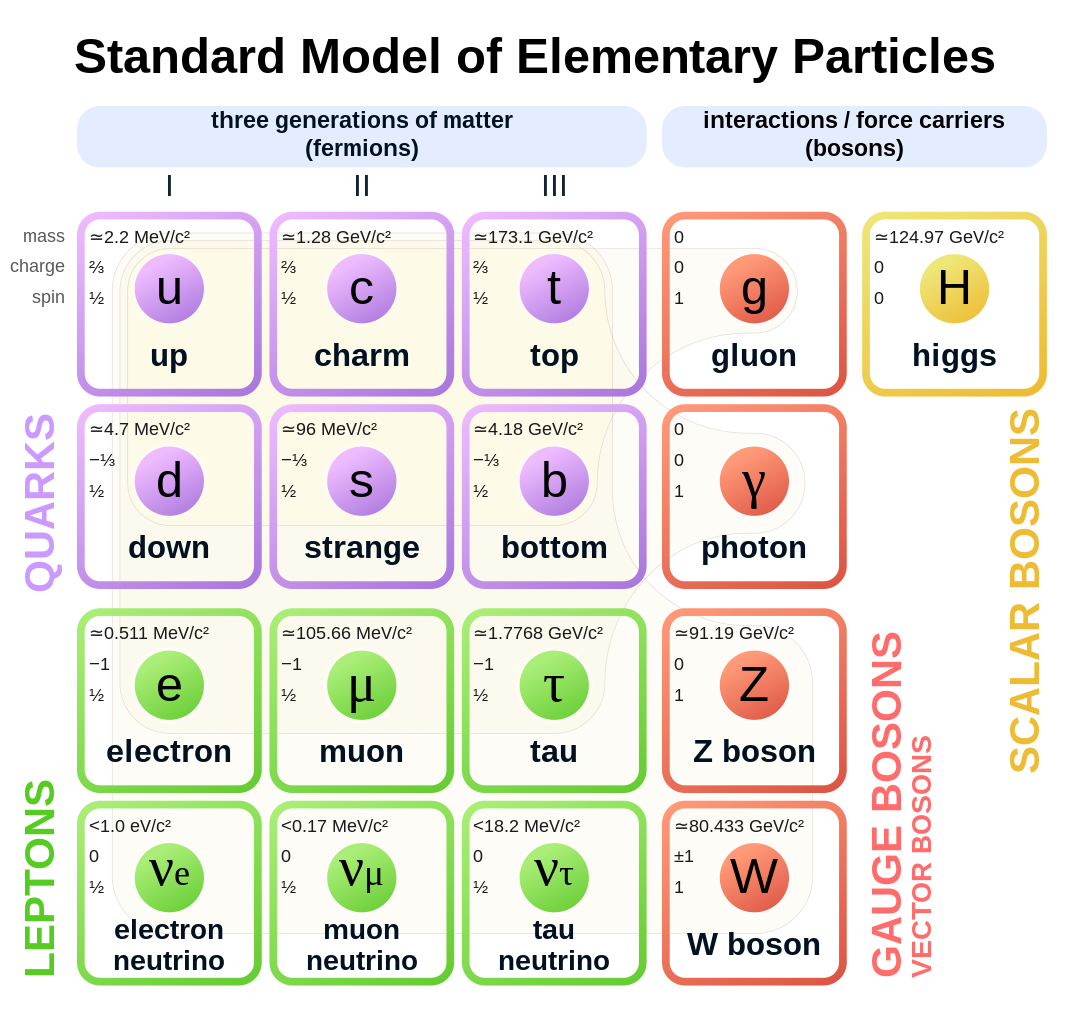
\includegraphics[width=0.98\textwidth]{figures/Standard_Model_of_Elementary_Particles.png}}
\legend{The elementary particles that are part of the Standard Model. Their mass, charge and spin are specified in their box. They are separated in the quarks, leptons, gauge bosons and scalar bosons.}
\source{https://bit.ly/2xk15fQ}
\end{figure}

\section{Quantum Chromodynamics}\label{sec:QCD}

The QCD is the theory of the strong interactions. It is a development from 50 years ago to explain the phenomena of the hadronic matter. The first developments of a theory for the strong interaction began with Murray Gell-Mann and George Zweig to describe the new $\Delta$ particles, the hyperons and the K mesons. Independently, they proposed that the observed hadrons were bound states of particles forming a SU(3) triplet. It was possible to predict new particles as well as explain the difference in the masses of the hadrons, with the quark model called ``eightfold way'' \cite{osti_4008239}.

Later, the color charge was added to the model to explain bound states with three of the same-flavor of quark, which could not exist because the wave function of such state should be anti-symmetric to obey the Pauli principle. The three color charges (red, green and blue) were introduced so that the wave function of the hadrons are anti-symmetric on the color indices.

The number of colors can be confirmed by examination of the cross section of electron-positron annihilation into hadrons, which depends on the square of the charges of the quarks and the number of colors. When comparing to the $e^+e^- \rightarrow \mu^+\mu^-$ annihilation\footnote{This is a naive approximation, and can be corrected by higher order perturbative QCD calculations.}
\begin{equation}
    R = \frac{\sigma(e^+e^- \rightarrow \text{hadrons})}{\sigma(e^+e^- \rightarrow \mu^+\mu^-)} = n_c \times \sum_q Q_q^2\,
\end{equation}
where $n_c$ is the number of colors, $Q$ is the electric charge and the subscript $q$ is the quark flavour. Figure \ref{fig:Rsigma} shows the measurement of R in electron-positron collisions.

\begin{figure}[!htm]{15cm}
\caption{Cross section and R in electron-positron collisions.}%
\label{fig:Rsigma}
\fbox{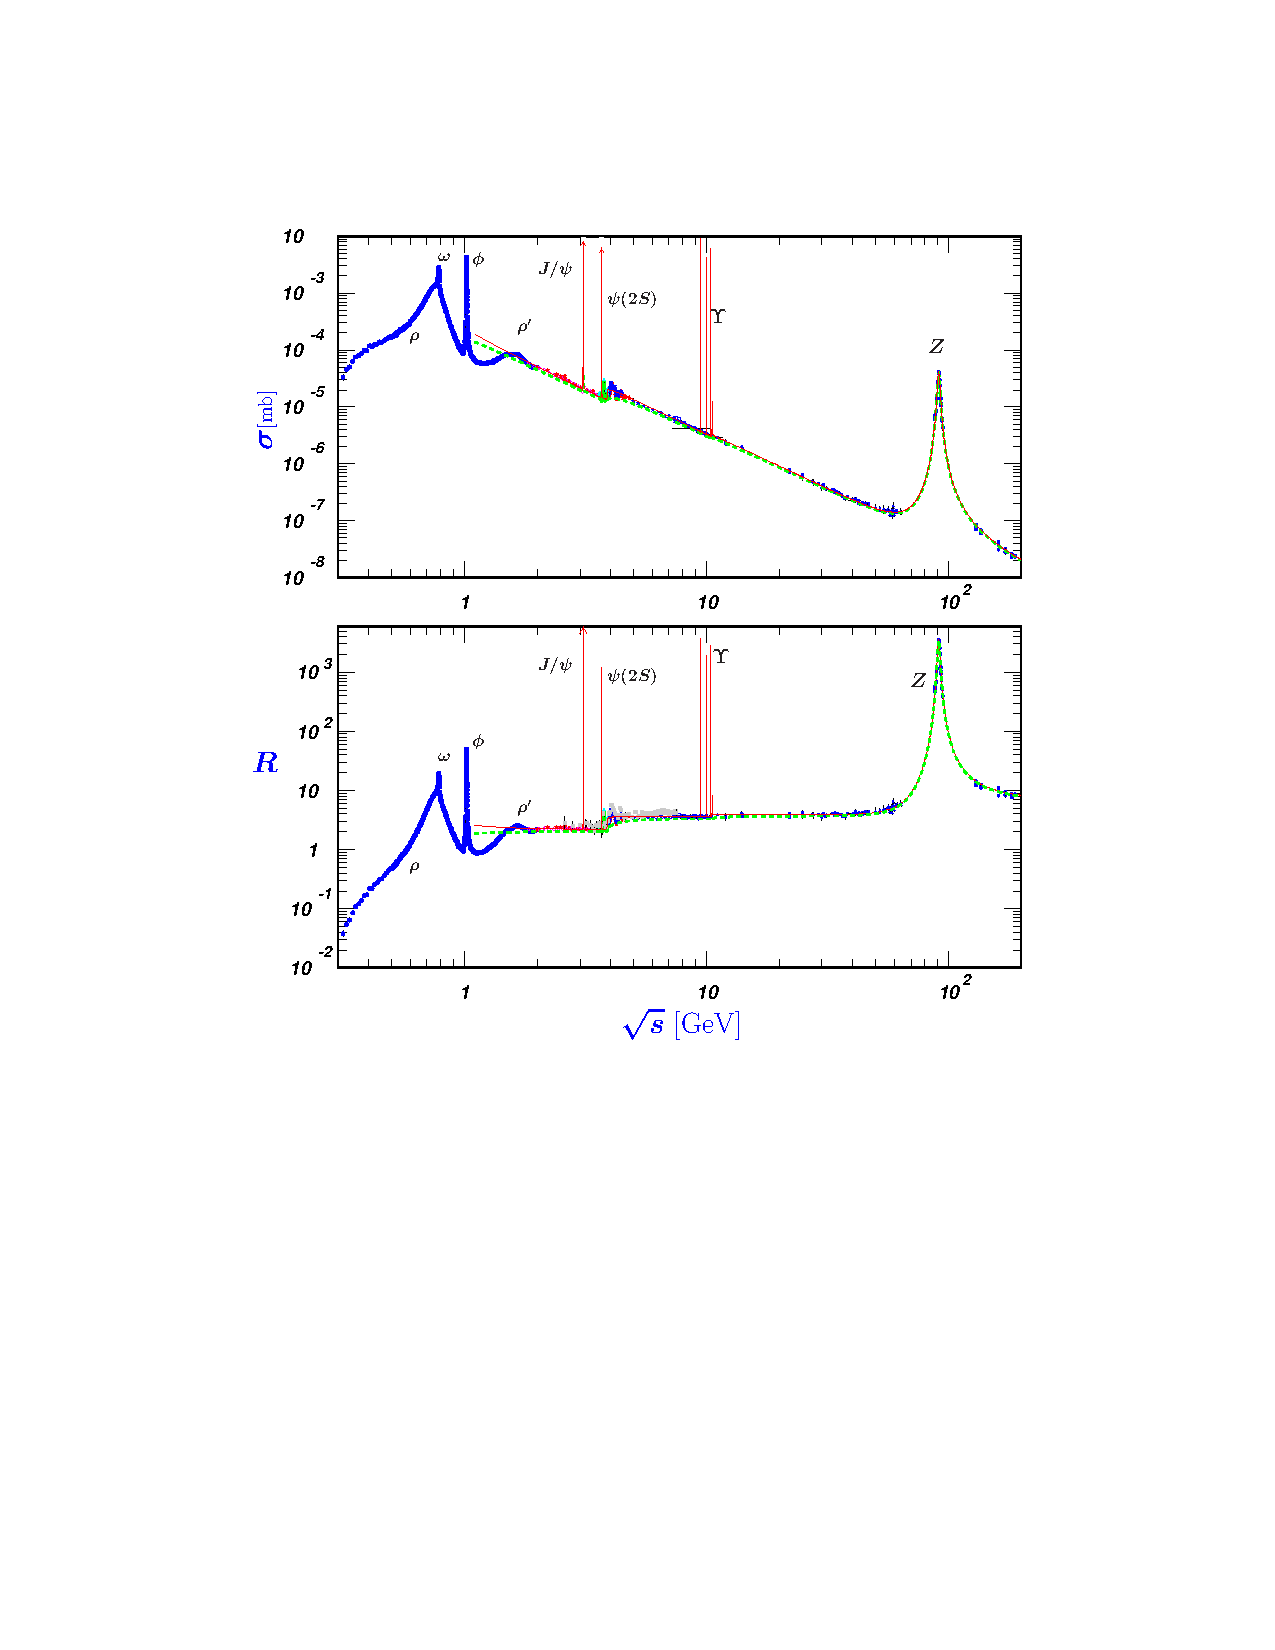
\includegraphics[width=0.8\textwidth]{figures/rpp2022-sigma_R_ee.pdf}}
\legend{Data (blue) on the total cross section of $\sigma(e^+e^- \rightarrow \text{hadrons})$ and the ratio $R = \sigma(e^+e^- \rightarrow \text{hadrons})/\sigma(e^+e^- \rightarrow \mu^+\mu^-)$. The broken curve (green) is a naive quark-parton model prediction, and the solid one (red) is 3-loop perturbative QCD prediction.}
\source{\cite{Workman:2022ynf}}
\end{figure}

The QCD was introduced to explain the quark model and its properties as a non-abelian SU(3) gauge theory \cite{Fritzsch:1973pi}. The Lagrangian of QCD is
\begin{equation}
    \mathcal{L}_{QCD} = \sum_f \overline{\psi}_{f,a}(i\delta_{ab}\slashed{D} - m_f\delta_{ab})\psi_{f,b} - \frac{1}{4}G^a_{\mu\nu}G^{a\mu\nu},
\end{equation}
where $\psi_{f, a}$ are quark field spinors for a quark of flavor q, mass $m_f$ and a color-index $a$ that runs from a = 1 to 3 (for red, green and blue). The $\slashed{D}$ is the covariant derivative, it contains the coupling between the quark and gluons fields 
\begin{equation}
    \slashed{D} = \gamma^\mu(\partial_\mu - i g_s A^a_\mu),
\end{equation}
where $A_\mu$ represents the gluon fields, which are generators of the SU(3) gauge group. The $g_s$ is the gauge coupling constant. The second term of the Lagrangian represents the kinetic term of the gluonic fields. They are expressed in terms of the field strength tensor $G^a_{\mu\nu}$ which is written in terms of the gluon fields as
\begin{equation}
    G^a_{\mu\nu} = \partial_\mu A^a_\nu - \partial_\nu A^a_\mu + g_sf^{abc}A^b_\mu A^c_\nu,
\end{equation}
where $f^{abc}$ are the structure constants of the SU(3) group. 

The coupling of the gluon fields with themselves occurs because the gluons carry color. Therefore, the QCD Feynman rules admit vertexes with three and four gluons as shown in Fig. \ref{fig:QCDvertex}. In comparison, there is only one vertex in the QED Feynman rules, with two fermions and one photon, since the photon caries no electric charge.

\begin{figure}[!htm]{15cm} 
\caption{QCD Feynman diagram vertex.}%
\label{fig:QCDvertex}
\fbox{
\begin{tabular}{ccc}
\begin{tabular}{c}
    \feynmandiagram [horizontal=a to b] { i1[particle=\(q\)] -- [fermion] a -- [fermion] i2[particle=\(q\)], a -- [gluon] b[particle=\(g\)],
    };
\end{tabular} & 
\begin{tabular}{c}
    \feynmandiagram [horizontal=a to b] { i1[particle=\(g\)] -- [gluon] a -- [gluon] i2[particle=\(g\)], a -- [gluon] b[particle=\(g\)],
    };
\end{tabular} & 
\begin{tabular}{c}
    \begin{tikzpicture}
        \begin{feynman}
            \vertex(a) ;
            \vertex[above left=of a](i1) {\(g\)};
            \vertex[below left=of a](i2) {\(g\)};
            \vertex[above right=of a](i3) {\(g\)};
            \vertex[below right=of a](i4) {\(g\)};
            \diagram*{
                (i1) -- [gluon] (a) -- [gluon] (i2),
                (i3) -- [gluon] (a) -- [gluon] (i4),
            };
        \end{feynman}
    \end{tikzpicture}
\end{tabular}
\end{tabular}
}
\legend{The allowed vertex in QCD. Besides the quark-gluon coupling represented by the first diagram from left to right, resembling the QED vertex, there are two more diagrams representing gluon-gluon interaction.}
\end{figure}

Only color-singlet (i.e. color neutral) particles are observed, therefore quarks and gluons are not directly detected free in the Nature. There are two types of hadrons which are commonly probed in experiments - the mesons, formed by the combination of a quark and a antiquark
\begin{equation}
    (q\overline q) \rightarrow (q_r \overline q_r + q_g \overline q_g + q_b \overline q_b)
\end{equation}
and the baryons formed by a combination of three quarks or three antiquarks
\begin{equation}
    (qqq) \rightarrow (q_r q_g q_b - q_g q_r q_b + q_b q_r q_g - q_r q_b q_g + q_g q_b q_r - q_b q_g q_r).
\end{equation}
Other kinds of states, such as tetraquarks or pentaquarks (4 and 5 quark and antiquark bound states, respectively, commonly called exotic) are possible \cite{Gell-Mann:1964ewy, Zweig:1964jf}, a list of such states observed in LHC can be found in \cite{LHCb-FIGURE-2021-001-report}. Also, gluon-gluon bound states are possible, known as glueball or gluonium, but were never observed \cite{Mathieu:2008me}. 

QCD has two very unique properties, asymptotic freedom and color confinement. Asymptotic freedom states that in the limit of high energies, the coupling constant of the QCD ($\alpha_s = \frac{g_s}{4\pi}$) becomes small \cite{PhysRevLett.30.1343, PhysRevLett.30.1346} and it can be treated perturbatively. Measurements of $\alpha_s$ are shown in Figure \ref{fig:couplingQCD}, which illustrates this behavior. Color confinement express the fact that free quarks are not observed. It is understood as a consequence of gluon self-interaction and the consequent increase of potential energy due to the color field as two quarks in a hadron are separated.

\begin{figure}[!htm]{15cm}
\caption{QCD coupling constant.}%
\label{fig:couplingQCD}
\fbox{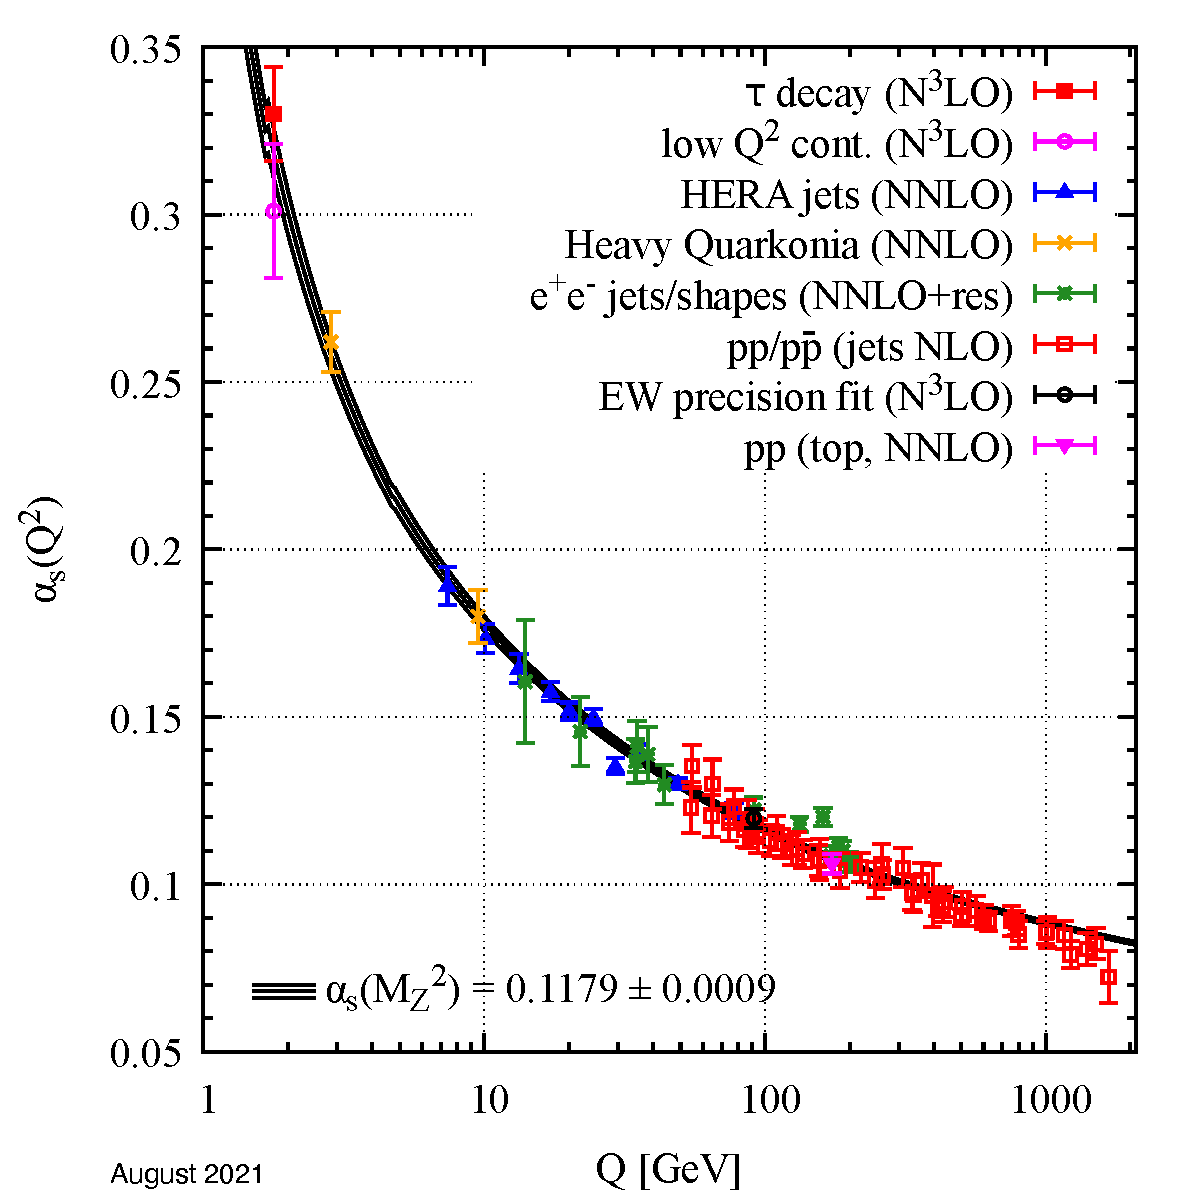
\includegraphics[width=0.8\textwidth]{figures/alphas-v-Q-2021.pdf}}
\legend{Summary of measurements of $\alpha_s$ as a function of the energy scale Q. The respective degree of QCD perturbation theory used in the extraction of $\alpha_s$ is indicated in brackets (NLO: next-to-leading order; NNLO: next-to-next-to-leading order; NNLO+res.: NNLO matched to a resummed calculation; N$^3$LO: next-to-NNLO)}
\source{\cite{Workman:2022ynf}}
\end{figure}

\section{Quarkonia}

The quarkonia are mesons made of a heavy quark and antiquark of the same flavour. The possible quarkonium states are the $c\overline{c}$, the charmonium, and $b\overline{b}$, the bottomonium. Light mesons (u, d and s) form physical quark-antiquark states\footnote{The $\eta$, $\eta^\prime$, and $\pi^0$ mesons.} but, because of their small mass, they are actually quantum mechanical mixtures of such states. Finally, the top quark quarkonium is not expected to be found, because, due to its very high mass, the top quark decays through electroweak interaction before a bound state can be formed, but there are some signatures that could be explored in the search for the toponium \cite{Fuks:2021xje}.

The special property of the quarkonia is that they form a bound-state with radius much lower than confinement scale, thus the QCD coupling constant has lower values, so that these particles can be treated perturbatively, which leads to states that are very similar to the electromagnetic particle-antiparticle systems \cite{Burgess:2006hbd}, the positronium and the muonium, from which the quarkonium name derives. Furthermore, because they are made of heavy quarks they form non-relativistic states, which are very well treated by a effective theory called NRQCD.

The $c\overline{c}$ and $b\overline{b}$ bound states may be classified with respect to their principal quantum number, $n$, angular momentum quantum numbers, $l$ and $m$, and spin quantum numbers, $s$ and $s_z$, using the same spectroscopic notation used in atoms. Figure \ref{fig:qq_spectrum} shows the quarkonium spectrum.

\begin{figure}[!htm]{15cm}
  \caption{Quarkonium spectrum.} 
  \label{fig:qq_spectrum}
  \subfloat[][]{\label{subfig:cc_spectrum}%
    \fbox{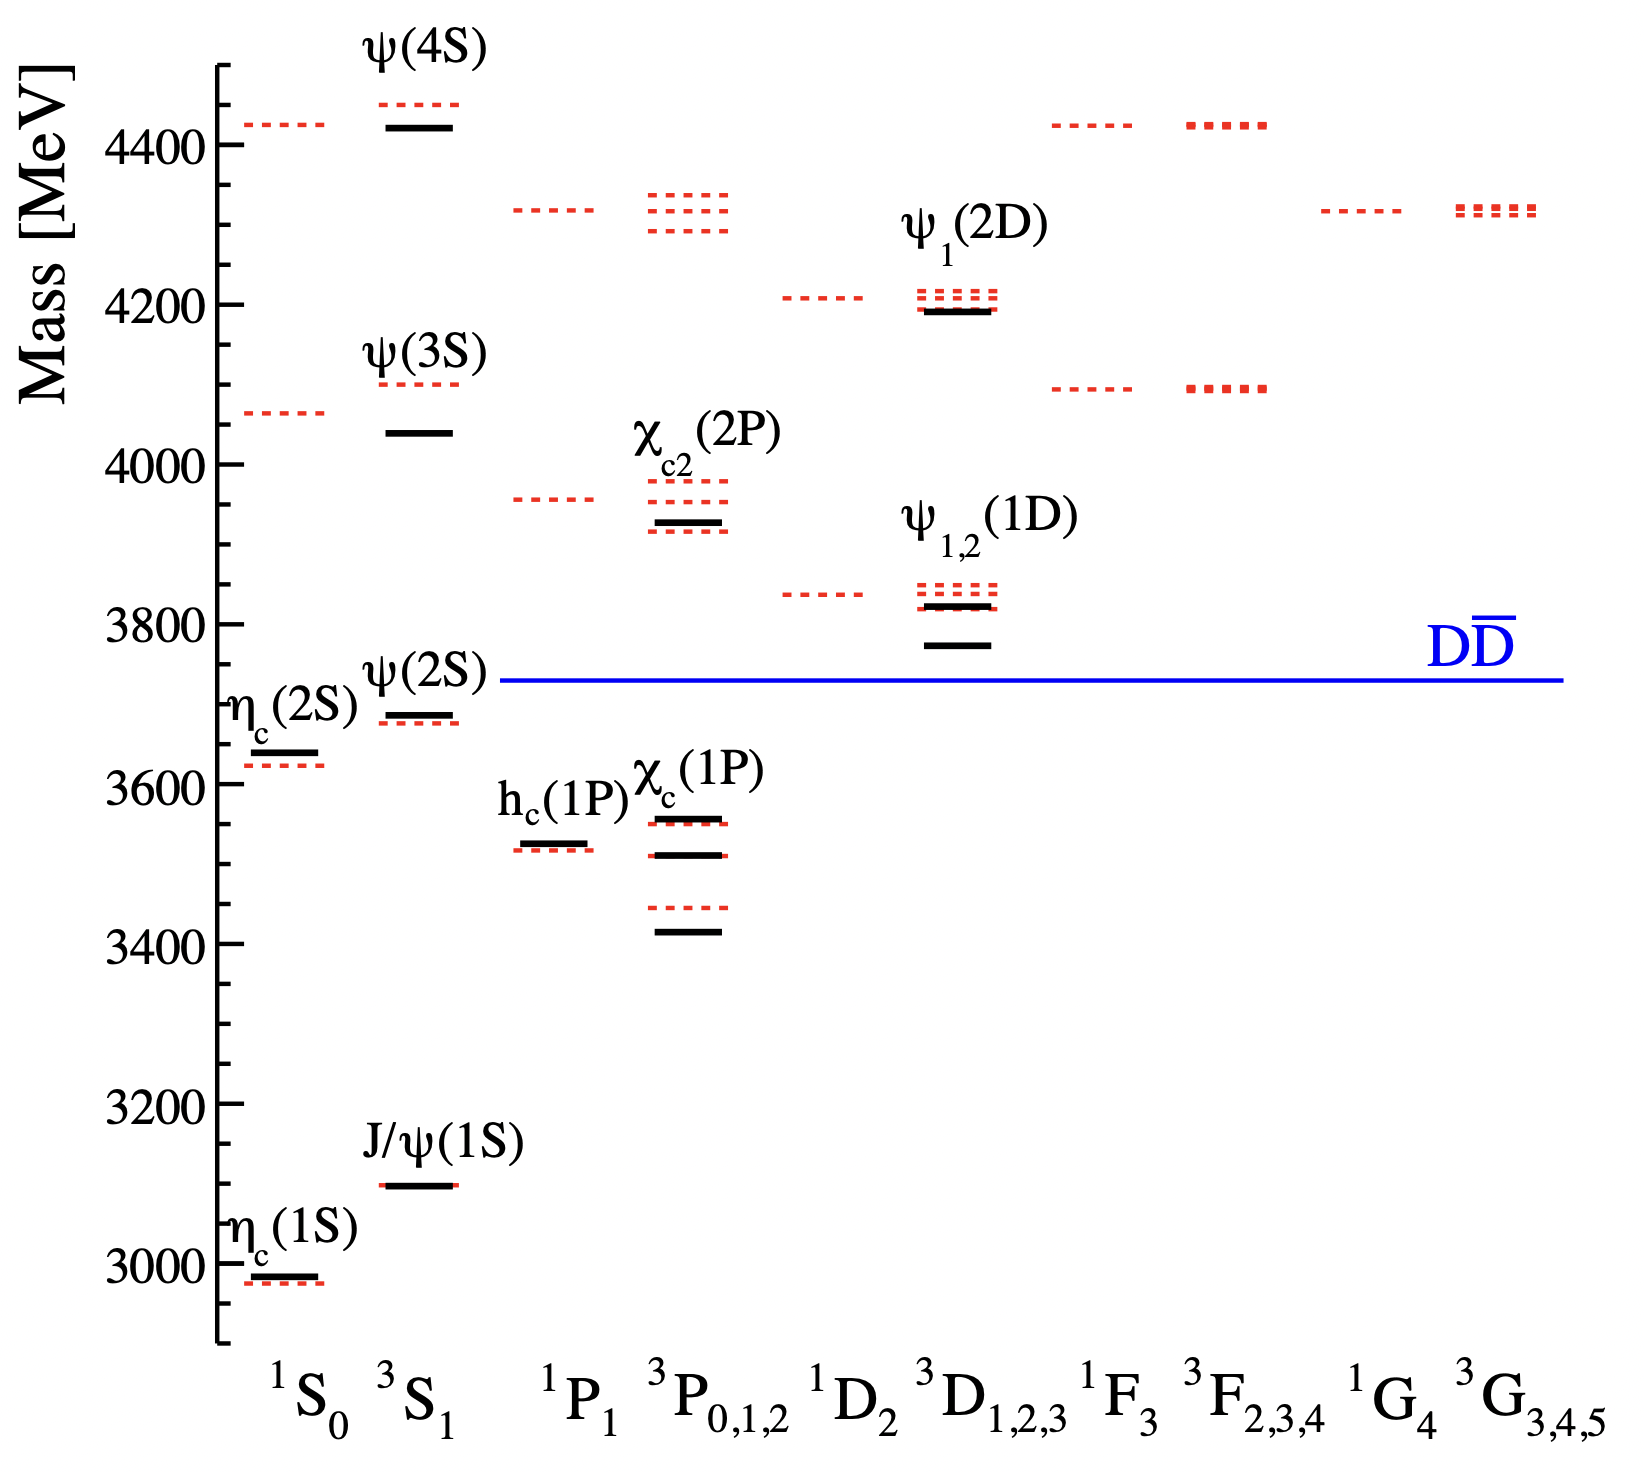
\includegraphics[width=0.45\textwidth]{figures/cc_spectrum.png}}}\hfill
  \subfloat[][]{\label{subfig:bb_spectrum}%
    \fbox{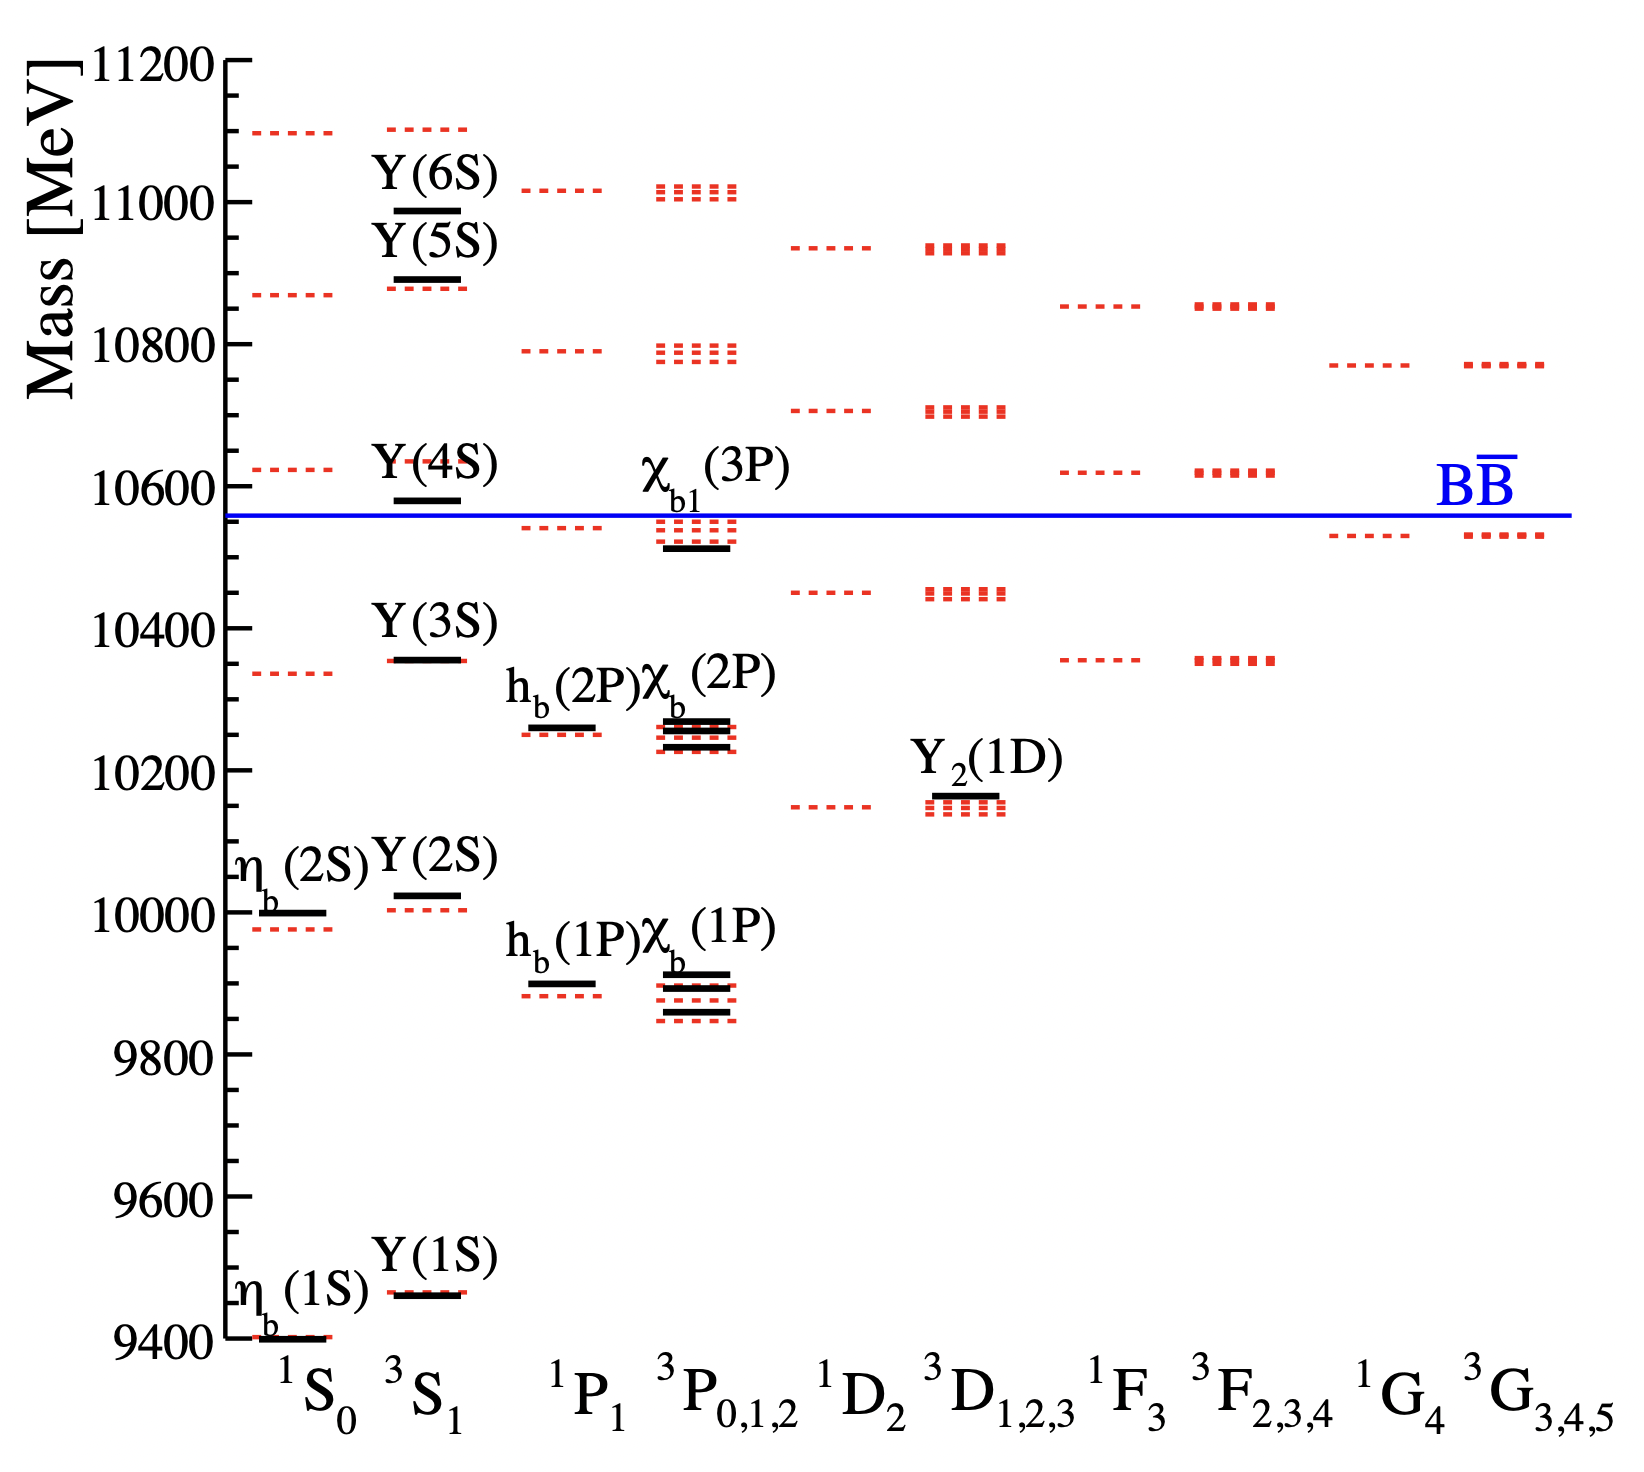
\includegraphics[width=0.45\textwidth]{figures/bb_spectrum.png}}}\\
  \legend{Current status of the charmonium (a) and bottomonium (b) spectra. The dashed lines indicate the expected states and their masses. The solid lines indicates the experimentally established quarkonia states. The open-flavor threshold is indicated in the blue line.}
  \source{\cite{RevModPhys.90.015003}}
\end{figure}

The discovery of the J/$\psi$, in 1974 \cite{E598:1974sol, SLAC-SP-017:1974ind}, allowed to identify the charm quark, confirming the quarks as real particles and not mathematical entities to explain the hadrons. This triggered many changes in the understanding of particle physics which is today known as November Revolution. Later, the $\Upsilon$ meson was discovered in 1977 \cite{E288:1977xhf}, the first particle containing b quarks.

Still today, the quarkonia are of very interest in particle physics, because they are easy to be treated experimentally and have high yields in the LHC energy scale. They appear as products of decays of exotic states \cite{CMS:2013jru, LHCb:2021uow, LHCb:2021vvq}, B mesons and Higgs boson \cite{ATLAS:2015vss} and can hint properties of the Quark-Gluon Plasma \cite{Matsui:1986dk, Wolschin:2016oua}.

\section{Multiple Parton Scattering}

Protons are not elementary particles, they are formed by a bound state of uud quarks, called valence quarks, the gluons that bind the valence quarks together and the sea quarks and antiquarks, which are formed by the interaction of the gluons in the protons. All of them are collectively referred to as partons.

Therefore, as opposed to the electron-positron collision, one cannot determine the initial states of a proton-proton (pp) collision and the calculation of the perturbative cross sections are determined be the factorization theorem \cite{Collins:1989gx}. If one parton from each proton interact, cross section can be determined as
\begin{equation}\label{eq:SPSxsec}
    \sigma_{A} = \sum_{i,j}\int dx_i \; dx_j \; f_i(x_i, \mu_F) \; f_j(x_j, \mu_F) \cdot \Hat{\sigma}_{i,j}^X(x_i, x_j, \mu_F)  
\end{equation}
where, $i$ and $j$ are the interacting partons, $x_i$ ($x_j$) is the momentum fraction carried by the parton $i$ ($j$), $f(x, \mu_F)$ is the parton distribution function (PDF), which is defined as the probability density for finding a parton with a certain longitudinal momentum fraction $x$ at factorization scale $\mu_F$ and $\Hat{\sigma}$ is the partonic cross section that can be calculated by the perturbative QCD (pQCD). The PDFs are the non-perturbative part of the Eq. \ref{eq:SPSxsec} and are determined experimentally \cite{NNPDF:2017mvq} and are shown in Fig. \ref{fig:NNLOPDFs}.

\begin{figure}[!htm]{15cm} 
\caption{NNLO Parton Distribution Functions.}%
\label{fig:NNLOPDFs}
\fbox{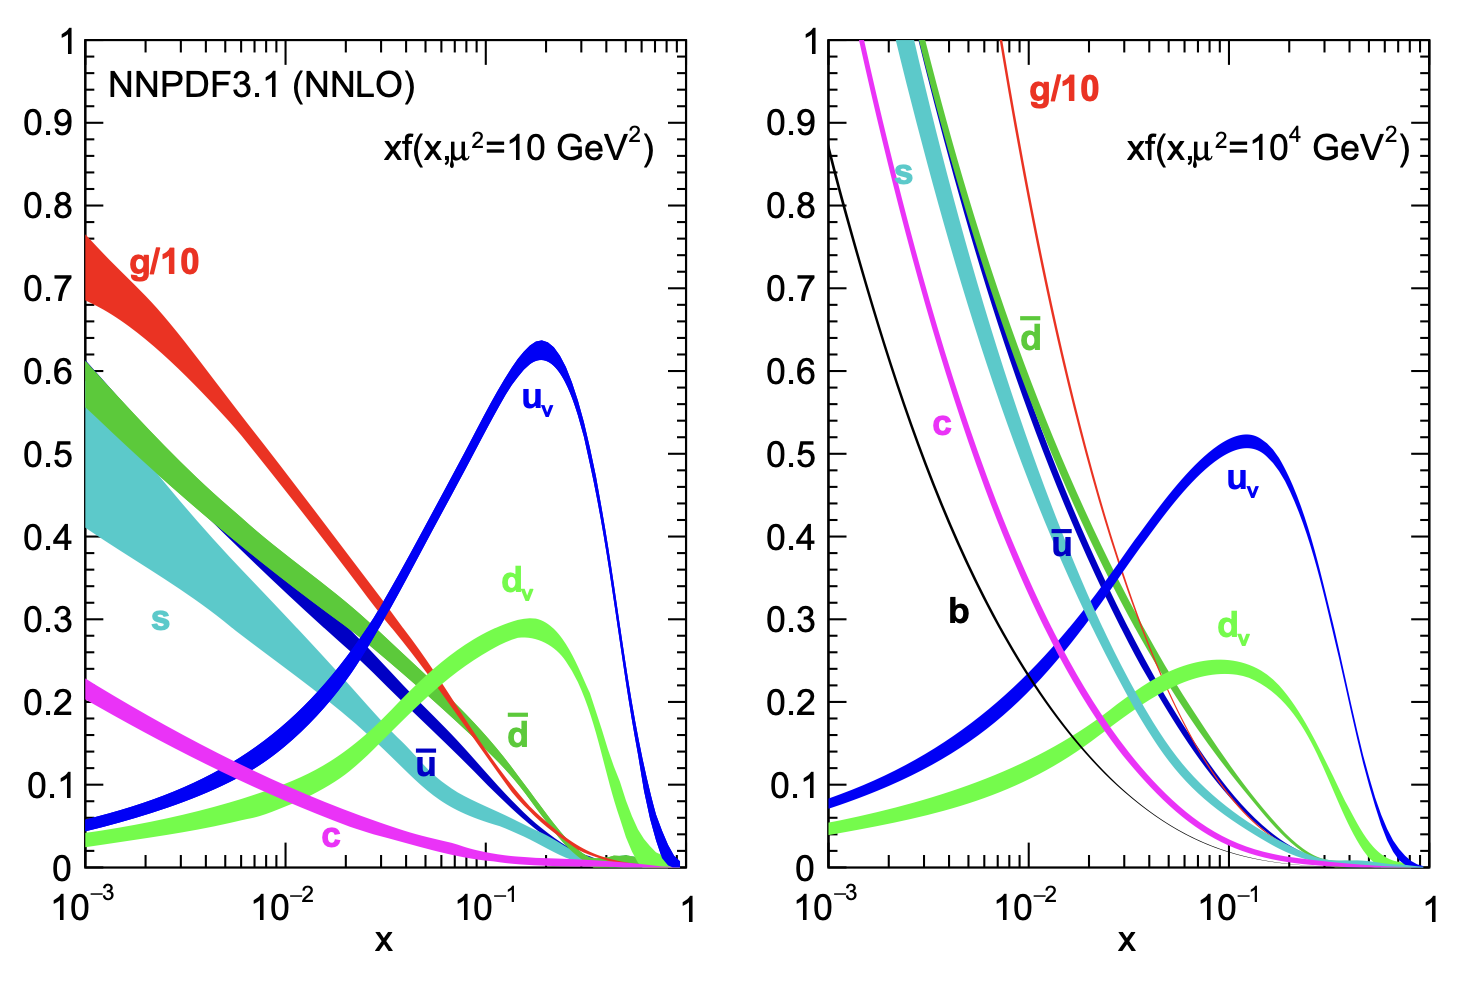
\includegraphics[width=0.9\textwidth]{figures/NNLO_PDFs.png}}
\legend{NNLO Parton distribution functions determined for $\mu_F^2 =$ 10 GeV$^2$ (left) and 10$^4$ GeV$^2$ (right)}
\source{\cite{NNPDF:2017mvq}}
\end{figure}

It is also possible that more than one parton from each proton take part in the process, giving rise to more than one hard interaction, a process known as Multiple Parton Scattering (MPS). In the MPS context, the pp interaction with one hard interaction is called Single Parton Scattering (SPS) and first extension is the Double Parton Scattering (DPS), where two hard interactions happen. Figure \ref{fig:SPSxDPS} shows the SPS and DPS examples.

\begin{figure}[!htm]{15cm}
  \caption{Single Parton Scattering and Double Parton Scattering sketches.} 
  \label{fig:SPSxDPS}
  \subfloat[][]{\label{subfig:SPS}%
    \fbox{
\begin{tikzpicture}
\begin{feynman}
\vertex(i1) {\(p\)};
\vertex[below=3cm of i1](i2) {\(p\)};
\vertex[blob, right=2cm of i1](h1) {};
\vertex[above=.15 of h1](h12) {};
\vertex[below=.15 of h1](h13) {};
\vertex[blob, right=2cm of i2](h2) {};
\vertex[above=.15 of h2](h22) {};
\vertex[below=.15 of h2](h23) {};
\vertex[blob, below right=2.12cm of h1](a) {};
\path (a) ++ (00:2) node[vertex] (o2);
\path (a.+30-|o2.center) node[vertex] (o1);
\path (a.-30-|o2.center) node[vertex] (o3);
\path (h1) ++ (00:2) node[vertex] (hf2);
\path (h1.+30-|hf2.center) node[vertex] (hf3);
\path (h1.+60-|hf2.center) node[vertex] (hf4);
\path (h2) ++ (00:2) node[vertex] (hf5);
\path (h2.-30-|hf4.center) node[vertex] (hf6);
\path (h2.-60-|hf4.center) node[vertex] (hf7);
\path (i1.+30-|h12.center) node[vertex] (i12);
\path (i1.-30-|h13.center) node[vertex] (i13);
\path (i2.+30-|h22.center) node[vertex] (i22);
\path (i2.-30-|h23.center) node[vertex] (i23);

\diagram* {
    (i1) -- [fermion] (h1) -- (a),
    (i1.+30) -- [fermion] (h12),
    (i1.-30) -- [fermion] (h13),
    (i2.+30) -- [fermion] (h22),
    (i2.-30) -- [fermion] (h23),
    (i2) -- [fermion] (h2) -- (a) -- (o2),
    (a.-30) -- (o3),
    (a.+30) -- (o1),
    (h1) -- [fermion] (hf2),
    (h1.+30) -- [fermion] (hf3),
    (h1.+60) -- [fermion] (hf4),
    (h2) -- [fermion] (hf5),
    (h2.-30) -- [fermion] (hf6),
    (h2.-60) -- [fermion] (hf7),
};
\end{feynman}
\end{tikzpicture}
    }}\hfill
  \subfloat[][]{\label{subfig:DPS}%
    \fbox{
\begin{tikzpicture}
\begin{feynman}
\vertex(i1) {\(p\)};
\vertex[below=3cm of i1](i2) {\(p\)};
\vertex[blob, right=2cm of i1](h1) {};
\vertex[above=.15 of h1](h12) {};
\vertex[below=.15 of h1](h13) {};
\vertex[blob, right=2cm of i2](h2) {};
\vertex[above=.15 of h2](h22) {};
\vertex[below=.15 of h2](h23) {};
\vertex[blob, below right=of h1](a) {};
\vertex[blob, above right=of h2](b) {};
\path (a) ++ (00:2) node[vertex] (o2);
\path (a.+30-|o2.center) node[vertex] (o1);
\path (a.-30-|o2.center) node[vertex] (o3);
\path (b) ++ (00:2) node[vertex] (o5);
\path (b.+30-|o5.center) node[vertex] (o4);
\path (b.-30-|o5.center) node[vertex] (o6);
\path (h1) ++ (00:2) node[vertex] (hf2);
\path (h1.+30-|hf2.center) node[vertex] (hf3);
\path (h1.+60-|hf2.center) node[vertex] (hf4);
\path (h2) ++ (00:2) node[vertex] (hf5);
\path (h2.-30-|hf4.center) node[vertex] (hf6);
\path (h2.-60-|hf4.center) node[vertex] (hf7);
\path (i1.+30-|h12.center) node[vertex] (i12);
\path (i1.-30-|h13.center) node[vertex] (i13);
\path (i2.+30-|h22.center) node[vertex] (i22);
\path (i2.-30-|h23.center) node[vertex] (i23);

\diagram* {
    (i1) -- [fermion] (h1) -- (a),
    (i1.+30) -- [fermion] (h12),
    (i1.-30) -- [fermion] (h13),
    (i2.+30) -- [fermion] (h22),
    (i2.-30) -- [fermion] (h23),
    (i2) -- [fermion] (h2) -- (a) -- (o2),
    (h1) -- (b),
    (h2) -- (b),
    (a.-30) -- (o3),
    (a.+30) -- (o1),
    (b.-30) -- (o6),
    (b.+30) -- (o4),
    (b) -- (o5),
    (h1) -- [fermion] (hf2),
    (h1.+30) -- [fermion] (hf3),
    (h1.+60) -- [fermion] (hf4),
    (h2) -- [fermion] (hf5),
    (h2.-30) -- [fermion] (hf6),
    (h2.-60) -- [fermion] (hf7),
};
\end{feynman}
\end{tikzpicture}
    }}\\
  \legend{A comparison of the Single Parton Scattering (a) and Double Parton Scattering (b). The difference between the two are the number of partons coming from each proton. The hadrons formed in (b) are uncorrelated, and have different kinematic distributions than (a)}
\end{figure}

The factorization can also be used in the MPS. For the DPS, the cross section is calculated by the formula \cite{gaunt2010double}
\begin{equation}\label{eq:DPSxsecfull}
\begin{split}
    \sigma_{AB}^{DPS} = \frac{m}{2} \sum_{i,j,k,l}\int & \Gamma_{ij}(x_1, x_2, b, \mu_1, \mu_2) \; \Hat{\sigma}^A_{ik}(x_1, x_1^\prime, \mu_1) \; \Hat{\sigma}_{jl}^B(x_2, x_2^\prime, \mu_2) \\ & \times \Gamma_{kl}(x_1^\prime, x_2^\prime, b, \mu_1, \mu_2) \; dx_1\; dx_2\; dx_1^\prime\; dx_2^\prime\; d^2b,
\end{split}
\end{equation}
where the $m$ is a double count factor, m equals 1 if process A = process B and 2 otherwise. The $\Gamma_{ij}(x_1, x_1, b, \mu_1, \mu_2)$ are the generalized double parton distributions. They may be interpreted as the inclusive probability distributions to find a parton i with longitudinal momentum fraction $x_1$ at scale $\mu_1$ in the proton, in addition to a parton j with longitudinal momentum fraction $x_2$ at scale $\mu_2$, with the two partons separated by a transverse distance b. And finally the $\Hat{\sigma}$ is the parton-level cross section.

The multi-parton PDFs should depend on all the possible correlations between partons, such as color and flavour interactions as well as spatial and kinematics correlations. Currently there is no theoretical model capable to describe its phenomenology. So, as a simplification to the model, it is assumed that the $\Gamma_{ij}$ can be separated in two components, representing the longitudinal and transverse components
\begin{equation}
    \Gamma_{ij}(x_1, x_2, b, \mu_1, \mu_2) = D_{ij}(x_1, x_2, \mu_1, \mu_2)\cdot F(b).
\end{equation}

The correlations in the transverse plane are very significant - as they must bind the two partons together within the same hadron. On the other hand, the correlations in the longitudinal plane are typically ignored with the assumption that, at least for small $x_i$ values the longitudinal momenta correlations are small\footnote{At LHC energy scale, the fraction of partons with small $x$ is large.} \cite{gaunt2010double}. Therefore, $\Gamma_{ij}$ is taken as the product of the single parton distribution functions $f_i$ and $f_j$
\begin{equation}\label{eq:simpdPDF}
    \Gamma_{ij}(x_1, x_2, b, \mu_1, \mu_2) = f_j(x_1, \mu_1) \cdot f_i(x_2, \mu_2) \cdot F(b).
\end{equation}

Under those simplifications, the DPS cross section can be expressed in terms of the SPS cross sections by plugging Eq. \ref{eq:simpdPDF} in \ref{eq:DPSxsecfull}
\begin{equation}
    \sigma_{AB}^{DPS} = \frac{m}{2} \frac{\sigma_A^{SPS} \cdot \sigma_B^{SPS}}{\sigma_{eff}},
\end{equation}
where $m$ is one if $A = B$ and two if $A \neq  B$, $\sigma^{SPS}_A$ has the same formula from Eq. \ref{eq:SPSxsec}. The $\sigma_{eff}$ is written as
\begin{equation}\label{eq:sigmaeff}
    \sigma_{eff} = \left[ \int d^2b (F(b))^2 \right]^{-1}
\end{equation}
and it is a parameter characterizes the effective spatial area of the parton-parton interactions. Figure \ref{fig:sigmaeff_measurements} shows a summary of measurements of $\sigma_{eff}$ done by many experiments \cite{afs1987double,alitti1991study,abe1993study,cdf1997double,abazov2010double,aaij2012observation,aad2013measurement,chatrchyan2014study,abazov2014double,abazov2014observation,alconada2015observation,aaboud2016study,aaij2016production,abazov2016study,abazov2016evidence,aaij2017measurement,atlas2017measurement,khachatryan2017observation,sirunyan2018constraints}.

\begin{figure}[!htm]{15cm} 
\caption{Measurements and limits on the $\sigma_{eff}$.}%
\label{fig:sigmaeff_measurements}
\fbox{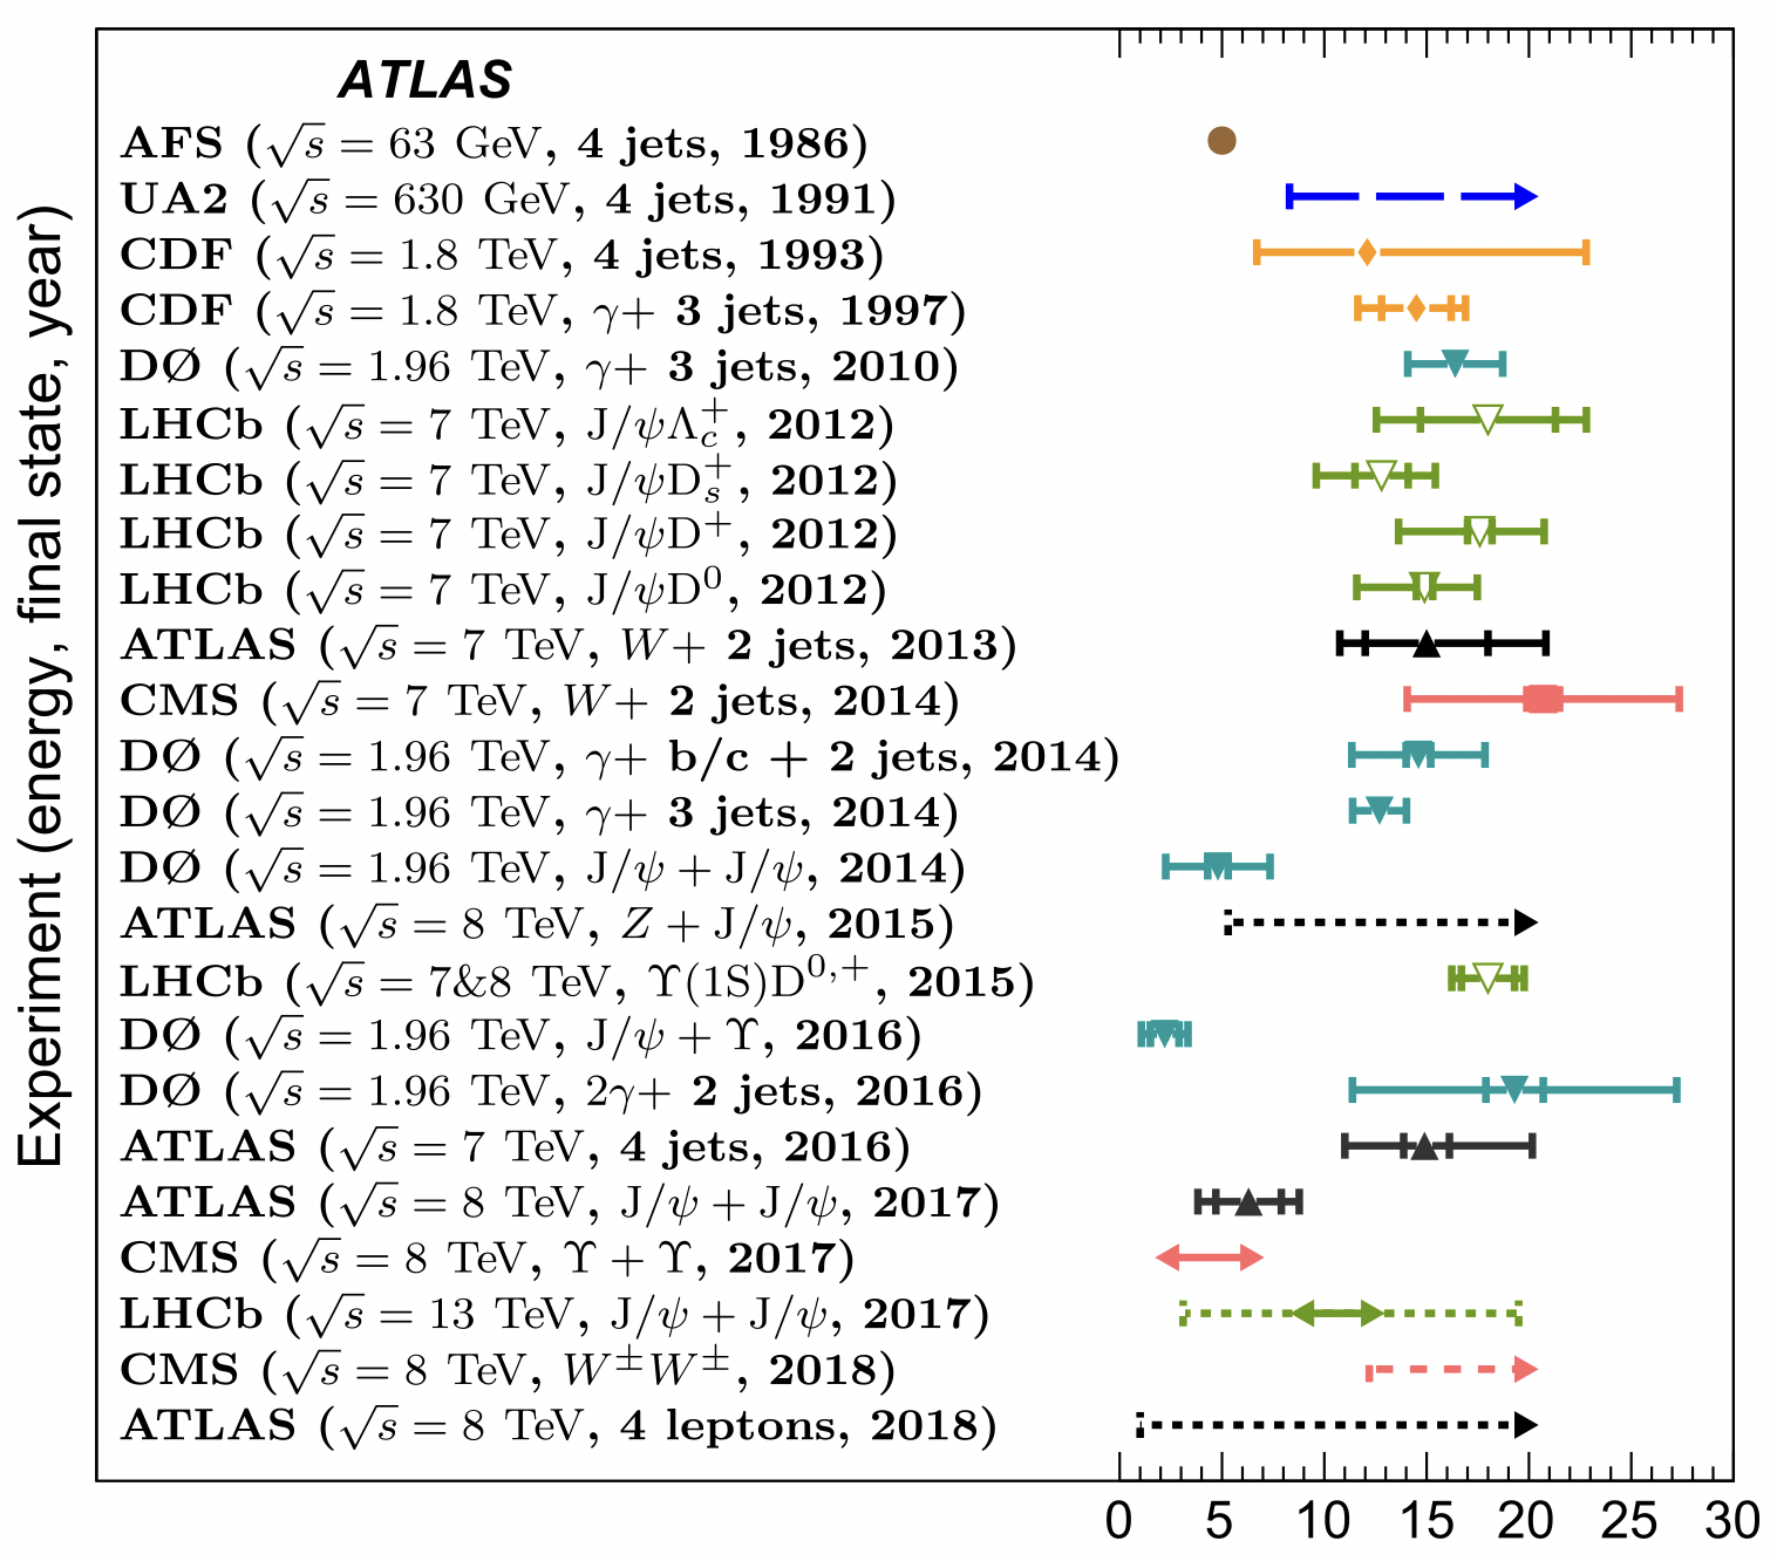
\includegraphics[width=0.68\textwidth]{figures/sigma_eff_measurements.png}}
\legend{Summary of measurements and limits on the $\sigma_{eff}$ determined by many experiments \cite{afs1987double,alitti1991study,abe1993study,cdf1997double,abazov2010double,aaij2012observation,aad2013measurement,chatrchyan2014study,abazov2014double,abazov2014observation,alconada2015observation,aaboud2016study,aaij2016production,abazov2016study,abazov2016evidence,aaij2017measurement,atlas2017measurement,khachatryan2017observation,sirunyan2018constraints}.}
\source{\cite{ATLAS:2018zbr}}
\end{figure}

The MPS is of great interest in the experiments as it can be a important contribution to background in multiparticle final-state processes. In high energy experiments, the MPS contribution is large, and can even overtake the SPS one \cite{Luszczak:2011zp}. Figure \ref{fig:SPSvsDPS} show the contribution of SPS and DPS to $c \bar c$ production, it is possible to see that at high enough center-of-mass energy, the DPS contribution is larger than SPS.

\begin{figure}[!htm]{15cm} 
\caption{Total LO $c \bar{c}$ cross section for SPS and DPS as a function of $\sqrt{s}$.}%
\label{fig:SPSvsDPS}
\fbox{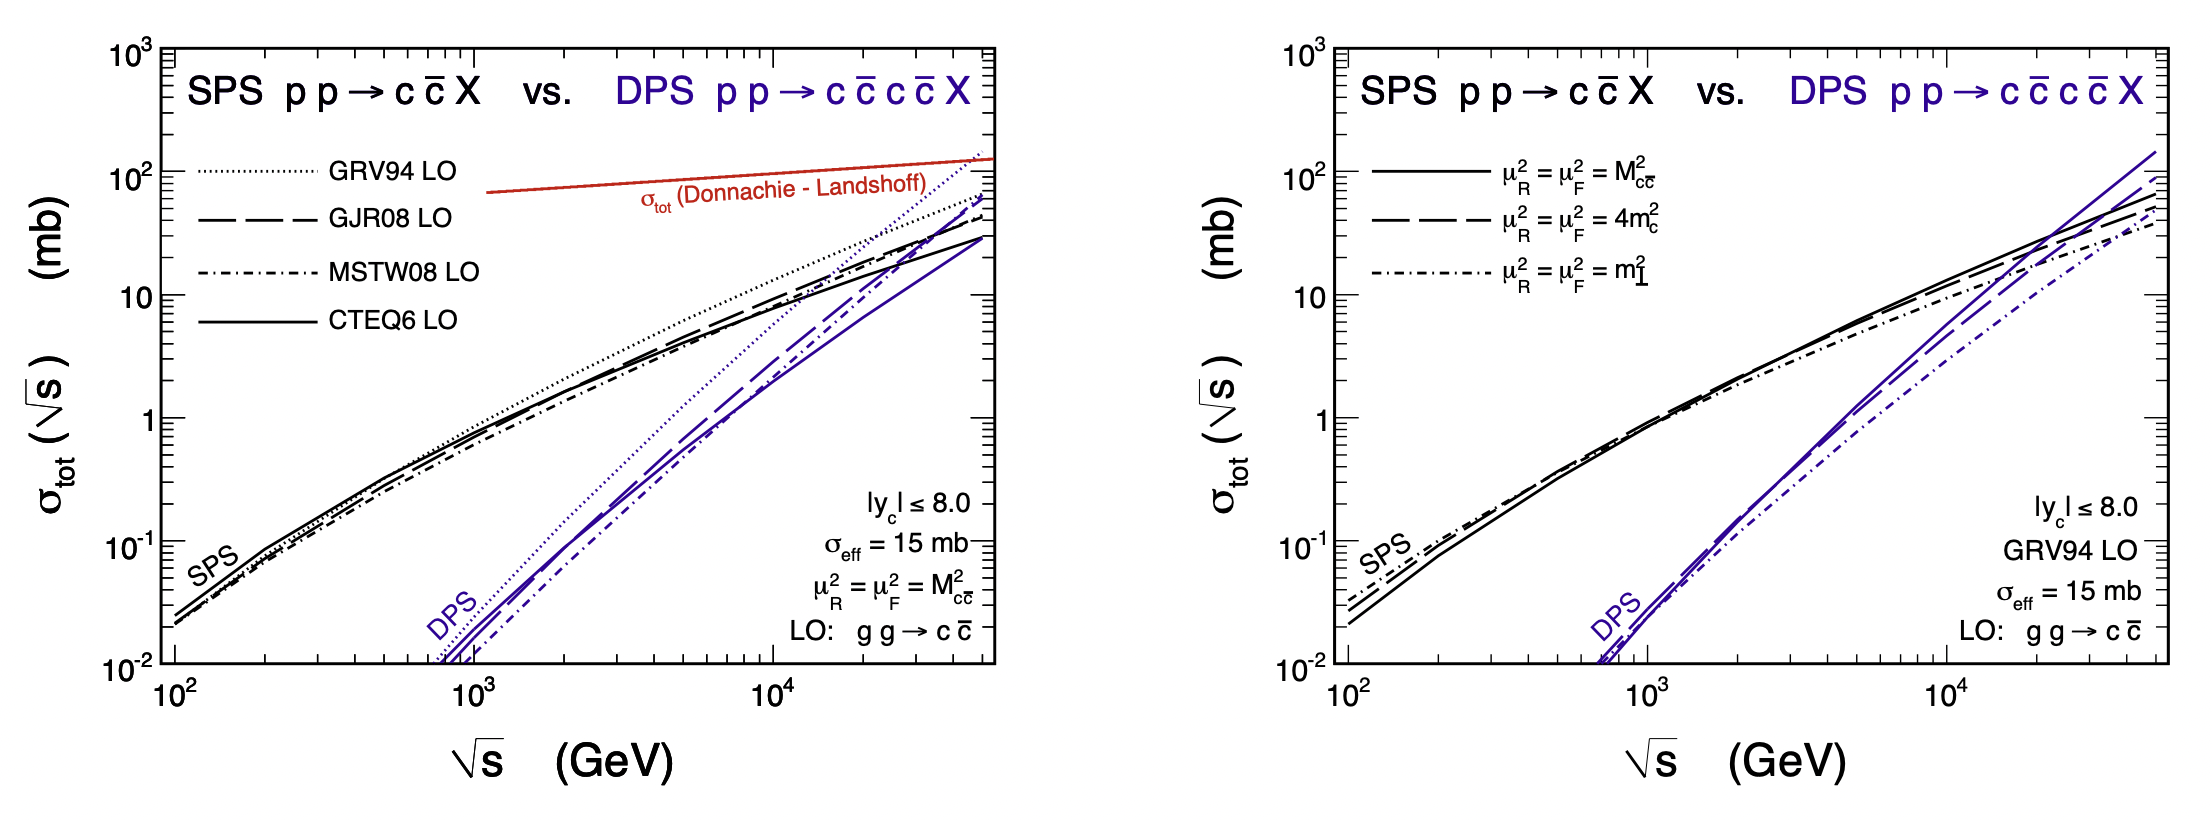
\includegraphics[width=0.98\textwidth]{figures/DPSvsSPS.png}}
\legend{Total LO cross section for SPS and DPS as a function of center-of-mass energy (left) and uncertainties due to the choice of (factorization, renormalisation) scales (right).}
\source{\cite{Luszczak:2011zp}}
\end{figure}

\section{Associated production of \texorpdfstring{$\Upsilon$}{Y } and Open Charm} \label{sec:theoryY+D}

The associated production of $\Upsilon$ and open charm is an interesting channel to investigate DPS \cite{Lansberg:2019adr} as it is expected that the SPS contribution is small. There is an experimental measurement from LHCb collaboration in 2015 \cite{aaij2016production} in which they concluded that the DPS cross section is at least 10 times higher than the SPS one, as expected from the theoretical study \cite{Berezhnoy:2015jga}. 

Under the hypothesis of the dominance of the DPS, LHCb extracted the values for the fiducial and effective cross section
\begin{equation}
\begin{split}
    BR_{Y \rightarrow \mu^+\mu^-} \times \sigma^{Y(1S)D^0}_{\sqrt{s}=7\, \text{TeV}} &= 155 \pm 21 (\text{stat}) \pm 7(\text{syst}) \, \text{pb}, \\
    BR_{Y \rightarrow \mu^+\mu^-} \times \sigma^{Y(1S)D^+}_{\sqrt{s}=7\, \text{TeV}} &= 82 \pm 19 (\text{stat}) \pm 5(\text{syst}) \, \text{pb}, \\
    BR_{Y \rightarrow \mu^+\mu^-} \times \sigma^{Y(1S)D^0}_{\sqrt{s}=8\, \text{TeV}} &= 250 \pm 28 (\text{stat}) \pm 11(\text{syst}) \, \text{pb}, \\
    BR_{Y \rightarrow \mu^+\mu^-} \times \sigma^{Y(1S)D^+}_{\sqrt{s}=8\, \text{TeV}} &= 80 \pm 16 (\text{stat}) \pm 5(\text{syst}) \, \text{pb}, \\
    \sigma_{eff}|_{\Upsilon(1S)D^0} &= 19.4 \pm 2.7 (\text{stat}) \pm 1.3 (\text{syst}) \, \text{mb}, \\
    \sigma_{eff}|_{\Upsilon(1S)D^+} &= 15.2 \pm 3.6 (\text{stat}) \pm 1.5 (\text{syst}) \, \text{mb}. 
\end{split}
\end{equation}

As the CMS phase space is very different from the LHCb, which covers only the frontal region ($2.0 < \eta < 5.0$). A measurement by the CMS collaboration can help to understand this channel in the central region, complementing the LHCb result, with the advantage of the higher luminosity recorded by CMS.

In order to perform a similar measurement in this thesis, the D$^{*\pm}$ will be used as charmed meson because of its good signal to background ratio and broad phase-space coverage. It has three different strong or electromagnetic decays \cite{Workman:2022ynf} with branching ratio (BR):
\begin{itemize}
    \item D$^{*+} \rightarrow$ D$^0 \pi^+$: BR = $67.7 \pm 0.5$ \%,
    \item D$^{*+} \rightarrow$ D$^+ \pi^0$: BR = $30.7 \pm 0.5$ \%,
    \item D$^{*+} \rightarrow$ D$^+ \gamma$: BR = $1.6 \pm 0.4$ \%,
\end{itemize}

For this thesis, the decay chosen is D$^0 \pi^+$. In addition to that, D$^0$ also decays through the weak interaction
\begin{equation*}
    \text{D}^0 \rightarrow K^- \pi^+\text{: BR = } 3.947\pm0.030\text{ \%},
\end{equation*}
adding to a total BR of 2.67 $\pm$ 0.03 \%. The mass difference of D$^{*+}$ and D$^0$ is small, so the momentum of the pion from the D$^{*+}$ is also small. For this reason, this pion is often referred to as pion ``slow'' ($\pi_s$).

From the quarkonium side, the first three states of $\Upsilon(nS)$ will be investigated. They decay electromagnetically to two leptons with opposite charge. The two muons channel (from here on, called dimuon) was chosen, with branching ratios of:
\begin{itemize}
    \item $\Upsilon(1S) \rightarrow \mu^+ \mu^-$: BR = $2.48 \pm 0.05$ \%,
    \item $\Upsilon(2S) \rightarrow \mu^+ \mu^-$: BR = $1.93 \pm 0.17$ \%,
    \item $\Upsilon(3S) \rightarrow \mu^+ \mu^-$: BR = $2.18 \pm 0.21$ \%.
\end{itemize}
The Tab. \ref{tab:pprops} summarizes the properties of the particles relevant to this work and Figs. \ref{fig:upsilontomumu} and \ref{fig:DstartoKpipi} show the Feynman diagrams for $b\bar b$ and D$^{*+}$ decays.

\begin{table}[!htbp]{15cm}
\caption{Properties of the particles considered in this work}\label{tab:pprops}
\begin{tabular}{ c | c | c | c | c }
    Particle & Quark content & Mass (MeV) & Lifetime (s) & $I^G(J^{PC})$ \\ \hline
    $\Upsilon(1S)$ & $b\bar b$ & $9460.30 \pm 0.26$     & - & $0^-(1^{--})$ \\ \hline
    $\Upsilon(2S)$ & $b\bar b$ & $10023.26 \pm 0.31$ & - & $0^-(1^{--})$ \\ \hline
    $\Upsilon(3S)$ & $b\bar b$ & $10355.2 \pm 0.5$   & - & $0^-(1^{--})$ \\ \hline
    $\mu^-$        & -         & $105.66$  & $2.197 \times 10^{-6}$ & $J = 1/2$ \\ \hline
    D$^{*+}$       & $c\bar d$ & $2010.26 \pm 0.05$  & - & $1/2(1^{-})$ \\ \hline
    D$^0$          & $c\bar u$ & $1864.84 \pm 0.05$  & $(410.3 \pm 1.0) \times 10^{-15}$ & $1/2(0^{-})$ \\ \hline
    K$^-$          & $s\bar u$ & $493.677 \pm 0.016$  & $(1.2379 \pm 0.0020) \times 10^{-8}$ & $1/2(0^{-})$ \\ \hline
    $\pi^+$        & $u\bar d$ & $139.57039 \pm 0.00018$  & $2.6033 \pm 0.0005 \times 10^{-8}$ & $1^-(0^{-})$ \\ \hline
  \end{tabular}
  \legend{Summary of the properties of the particles relevant to this work. The last column shows their the quantum numbers - I = isospin, G = G-symmetry, J = spin, P = Parity and C = charge conjugate. For the muon only the J quantum number is relevant, for the Ds and K, G and C are not present and for the $\pi$ only C is not present. The uncertainties on $\mu$ mass and lifetime were ommited.}
\source{\cite{Workman:2022ynf}}
\end{table}

\begin{figure}[!htm]{15cm}
\caption{Feynman Diagram for $b\bar b \rightarrow \mu^+\mu^-$.}%
\label{fig:upsilontomumu}
\fbox{
\feynmandiagram [large, horizontal=a to b] { 
i1[particle=\(b\)] -- [fermion] a -- [fermion] i2[particle=\(\overline b\)], a -- [photon, edge label=$\gamma$] b,
f1[particle=\(\mu^+\)] -- [fermion] b -- [fermion] f2[particle=\(\mu^-\)],
};
}
\legend{Example of Feynman diagram for $b\bar b$ annihilation to dimuon.}
\end{figure}

\begin{figure}[!htm]{15cm}
\caption{Feynman Diagram for D$^{*+} \rightarrow K^-\pi^+\pi_s^+$.}%
\label{fig:DstartoKpipi}
\fbox{
\begin{tikzpicture} 
\begin{feynman}
    \vertex (i1) {\(c\)};
    \vertex[below=3em of i1] (i2) {\(\overline d\)};
    \vertex[right=2cm of i2] (a);
    \vertex[right=2cm of a] (b);
    \vertex[right=2cm of b] (c) {\(\overline u\)};
    \vertex[above=3em of c] (d) {\(c\)};
    \vertex[right=1cm of d] (e);
    \vertex[right=2cm of e] (o3) {\(s\)};
    \vertex[below=3em of o3] (o4) {\(\overline u\)};
    \vertex[below right=2cm of a] (o1) {\(\overline d\)};
    \vertex[below right=2cm of b] (o2) {\(u\)};
    \vertex[above=of o3] (o6) {\(u\)};
    \vertex[above=of o6] (o5) {\(\overline d\)};
    \vertex[below left=of o5] (f);
    \vertex[below=1.5em of d] (x) {\(D^0\)};
    
    \diagram* {
        (i1) -- [fermion] (d) -- [fermion] (e) -- [fermion] (o3),
        (o4) -- [fermion] (c) -- [fermion] (b) -- [gluon] (a) -- [fermion] (i2), 
        (o1) -- [fermion] (a),
        (b) -- [fermion] (o2),
        (e) -- [boson, bend left, edge label=\(W^{+}\)] (f),
        (o5) -- [fermion] (f) -- [fermion] (o6)
    };

    \draw [decoration={brace}, decorate] (i2.south west) -- (i1.north west) node [pos=0.5, left] {\(D^{*+}\)};
    \draw [decoration={brace}, decorate] (o2.south east) -- (o1.south west) node [pos=0.5, below] {\(\pi_s^{+}\)};
    \draw [decoration={brace}, decorate] (o3.north east) -- (o4.south east) node [pos=0.5, right] {\(K^{-}\)};
    \draw [decoration={brace}, decorate] (o5.north east) -- (o6.south east) node [pos=0.5, right] {\(\pi^{+}\)};
    \draw {(x.center) ellipse (.35cm and 1cm)}; 
\end{feynman} 
\end{tikzpicture}
}
\legend{Example of Feynman diagram for D$^{*+} \rightarrow K^-\pi^+\pi^+$. The decay happens in to steps, first, the D$^{*+}$ decays into a D$^0$ and a $\pi_s^+$ and then, the D$^0$ further decays into a $K^-$ and a $\pi^+$.}
\end{figure}

\chapter{Experimental setup} \label{chap:experiment}
%================================================================

The goal of this chapter is to introduce the experimental setup used to acquire the data. The apparatus can be divided in two parts: the accelerator, the Large Hadron Collider (LHC), which will be discussed in the section \ref{sec:LHC} and the particle detector, the Compact Muon Solenoid (CMS), which will be discussed in the section \ref{sec:CMS}.

\section{The Large Hadron Collider}\label{sec:LHC}

The LHC is the world most powerful particle accelerator and collider. It is  situated at CERN in the border of Switzerland and France inside the tunnel of 26.7 km extension, in which the Large Electron-Positron collider, LEP, was built. It is designed to collide two proton beams with centre-of-mass energy of 14 TeV in a peak instantaneous luminosity of $10^{34} \; cm^{-2} s^{-1}$. Up to Run 2, the maximum centre-of mass energy achieved was 13 TeV and the instantaneous luminosity was double the nominal $2 \cdot 10^{34} \; cm^{-2} s^{-1}$. It can also collide heavy ions (Pb) \cite{Evans_2008}.

To achieve such numbers, the protons are first accelerated to 450 GeV before being injected to the machine. The injector chain is pictured in the Figure \ref{fig:acc_complex}, it follows the sequence: Linac4\footnote{Linac2 was used up to Run 2 in the injector chain, from 2020 it was replaced by Linac4} -- Proton Synchrotron Booster (PSB) -- Proton Synchrotron (PS) -- Super Proton Synchrotron (SPS). 

\begin{figure}[!htm]{15cm}
\caption{The CERN Accelerator Complex}%
\label{fig:acc_complex}
\fbox{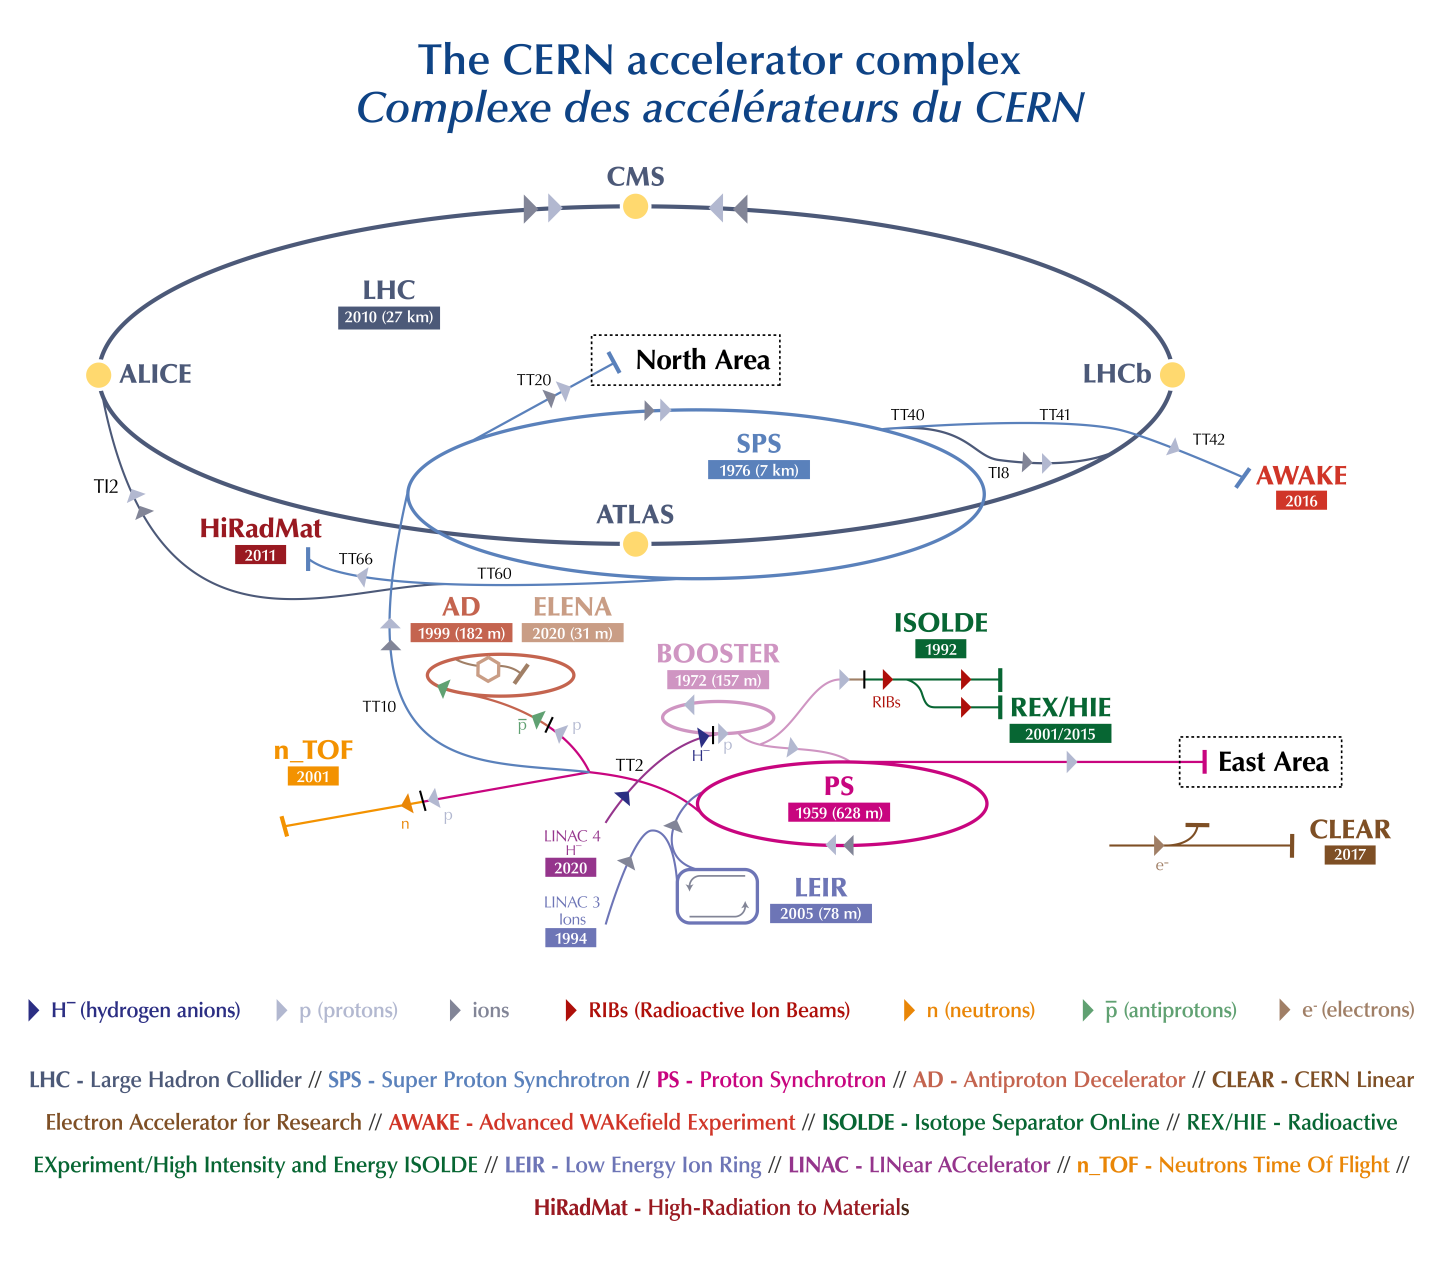
\includegraphics[width=0.9\hsize]{figures/acc_complex.png}}
\legend{All the machines that compose the CERN accelerator complex. The LHC is the last ring colored in dark blue.}
\source{\cite{Mobs:2684277}}
\end{figure}

In the LHC, the protons injected are divided into two tubes and are accelerated from 450 GeV to 6.5 TeV\footnote{In Run 2, this amounts to $\sqrt{s} = 13 \; TeV$. For Run 3 it is expected 6.8 TeV per beam or $\sqrt{s} = 13.6 \; TeV$}. The acceleration is accomplished by 16 radiofrequency (RF) cavities (8 per beam), the trajectory is maintained by 1232 dipoles placed along the tunnel, quadrupoles are also used to squeeze and focus the beam. All magnets are made of superconducting coils to reduce energy losses.

When the beams reach 6.5 TeV, they are directed to the interaction points (IP) by the insertion magnets, which also squeeze further the beams so that they collide. In the IPs are installed the LHC experiments, which are the following:

\begin{itemize}
    \item \textbf{ALICE (A Large Ion Collider Experiment):} Located at the P2, it is a general purpose detector specialized in heavy ion collisions. It focuses on QCD, the strong-interaction sector of the Standard Model \cite{ALICE:2008ngc}.
    \item \textbf{ATLAS (A Toroidal LHC Apparatus):} Located at P1 it is a general purpose detector designed to cope with the high collision rates of LHC and focus in various aspects of the SM and BSM (Beyond Standard Model) physics in the LHC energy scale \cite{ATLAS:2008xda}.
    \item \textbf{CMS (Compact Muon Solenoid):} Located at P5, it is a general purpose detector such as ATLAS, it is going to be further explored in the section \ref{sec:CMS} \cite{CMS:2008xjf}.
    \item \textbf{LHCb (Large Hadron Collider beauty):} Located at P8, it is an experiment focused in heavy flavour physics. Its goal is to look for indirect evidence of new physics in CP violation and rare decays of beauty and charm hadrons \cite{LHCb:2008vvz}.
\end{itemize}

\subsection{Luminosity and the HL-LHC}

One of the most important parameters of an accelerator is the instantaneous luminosity it can deliver. It is defined as
\begin{equation}
    \mathcal{L} = \frac{1}{\sigma_i} \frac{dN_i}{dt},
\end{equation}
where $\mathcal{L}$ is the instantaneous luminosity, $N_i$ is the number of events of the i-labeled process and $\sigma_i$ is the cross section of the process i. The integrated luminosity (L) is the integration in time of the instantaneous luminosity. Therefore, the number of events delivered by the accelerator is
\begin{equation}
    N_i = \sigma_i L.
\end{equation}

The integrated luminosity delivered by the LHC to the CMS detector in the course of the Run 1 and Run 2 (2010 to 2018) is presented in Figure \ref{fig:int_lumi}.

\begin{figure}[!htm]{15cm}
\caption{Integrated Luminosity delivered to CMS}%
\label{fig:int_lumi}
\fbox{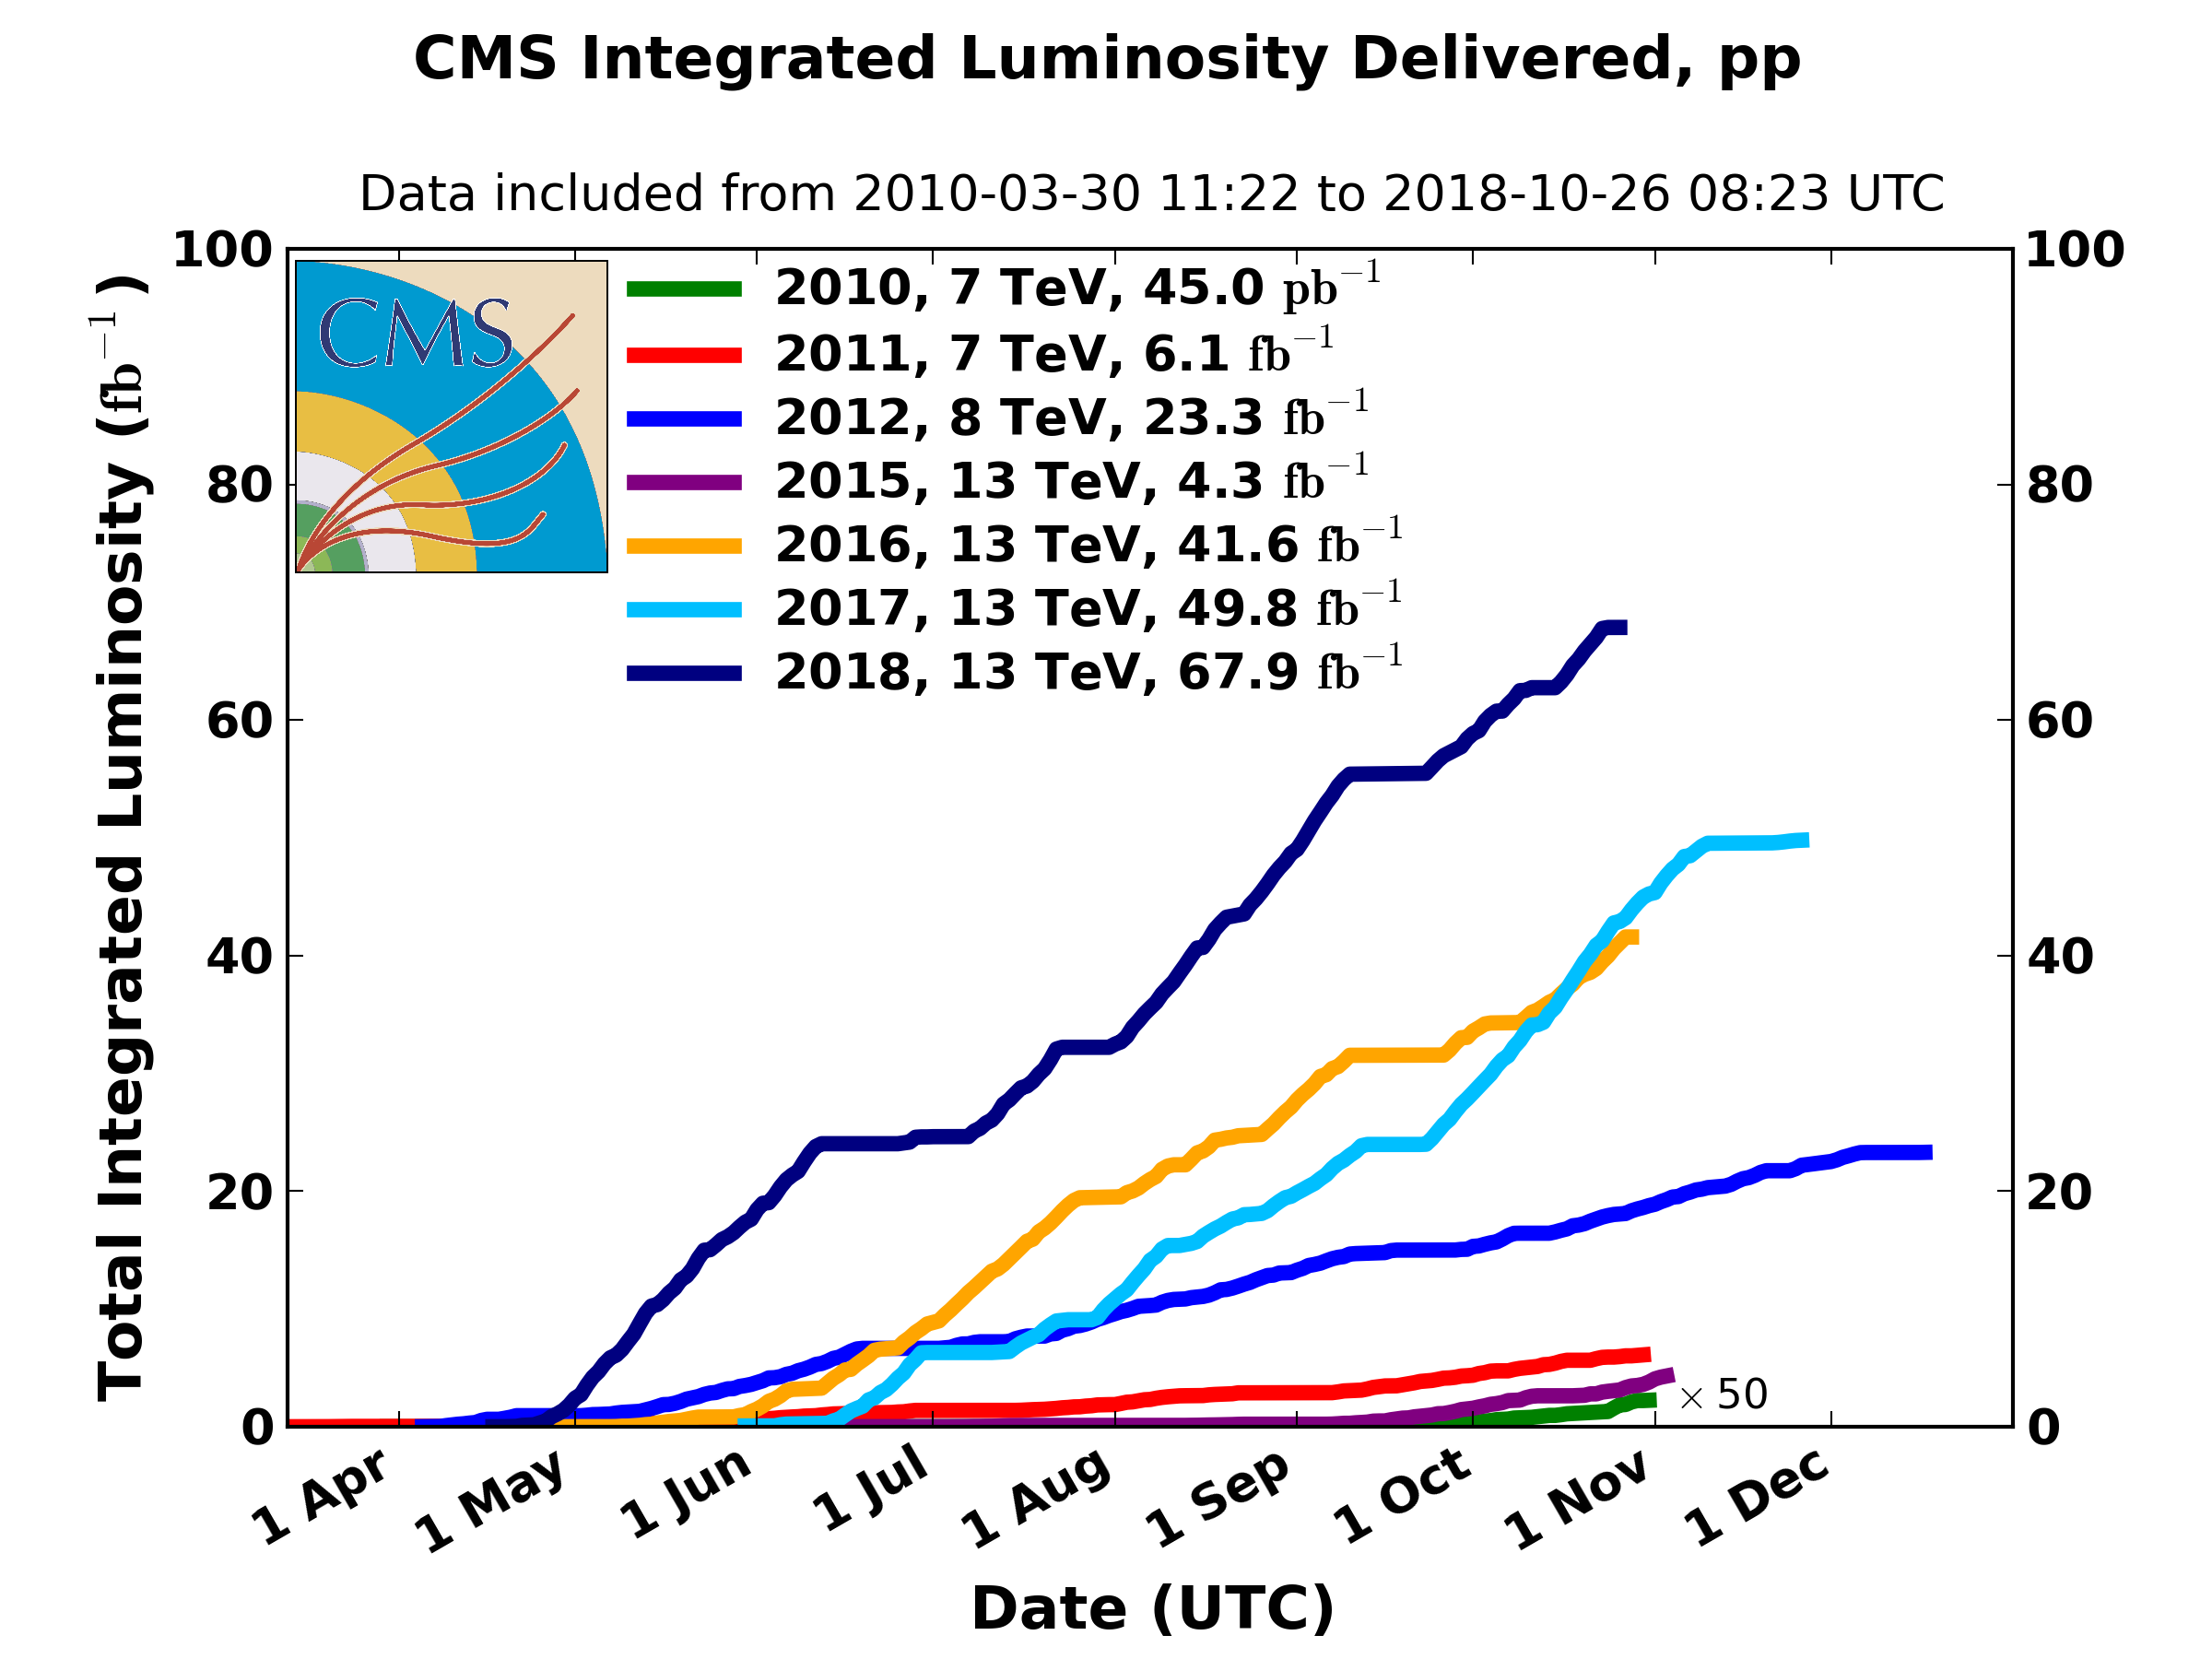
\includegraphics[width=0.7\hsize]{figures/int_lumi_cumulative_pp.png}}
\legend{The integrated luminosity delivered to CMS by the LHC from 2010 to 2018.}
\source{https://twiki.cern.ch/twiki/bin/view/CMSPublic/LumiPublicResults}
\end{figure}

The luminosity is very important to the statistics collected, therefore the HL-LHC project was proposed and accepted by the EU Strategy Report for High Energy Physics and the CERN Council. Its goal is to increase the peak instantaneous luminosity by a factor of 5 to extend the possibility of new discoveries and maximize the use of LHC \cite{Aberle:2749422}. It is expected a integrated luminosity of 3000 $fb^{-1}$ in 10-12 years. The current plan for the HL-LHC is in Figure \ref{fig:LHC_Plan}.

\begin{figure}[!htm]{15cm}
\caption{LHC/HL-LHC Plan}%
\label{fig:LHC_Plan}
\fbox{\includegraphics[width=0.9\hsize]{figures/LHC_plan.jpg}}
\legend{The plan for the LHC and HL-LHC from its start in 2011 to the expected end of the program in 2040.}
\source{https://hilumilhc.web.cern.ch/content/hl-lhc-project}
\end{figure}

\section{Compact Muon Solenoid Experiment}\label{sec:CMS}

The CMS is a multipurpose detector that investigates both proton-proton and lead-lead collisions at LHC. It has a cylindrical shape with 15 meters diameter and 22 m long, weighting 14\,000 tonnes, being the heaviest of the LHC experiments \cite{CMS:2008xjf}. It is divided into two distinct regions, the barrel, which refers to the central part and the endcap, for detection on the frontal region. Figure \ref{fig:cms_diagram} shows a schematic of the CMS detector and its components.

\begin{figure}[!htm]{15cm}
\caption{CMS Detector Cutaway Diagram}%
\label{fig:cms_diagram}
\fbox{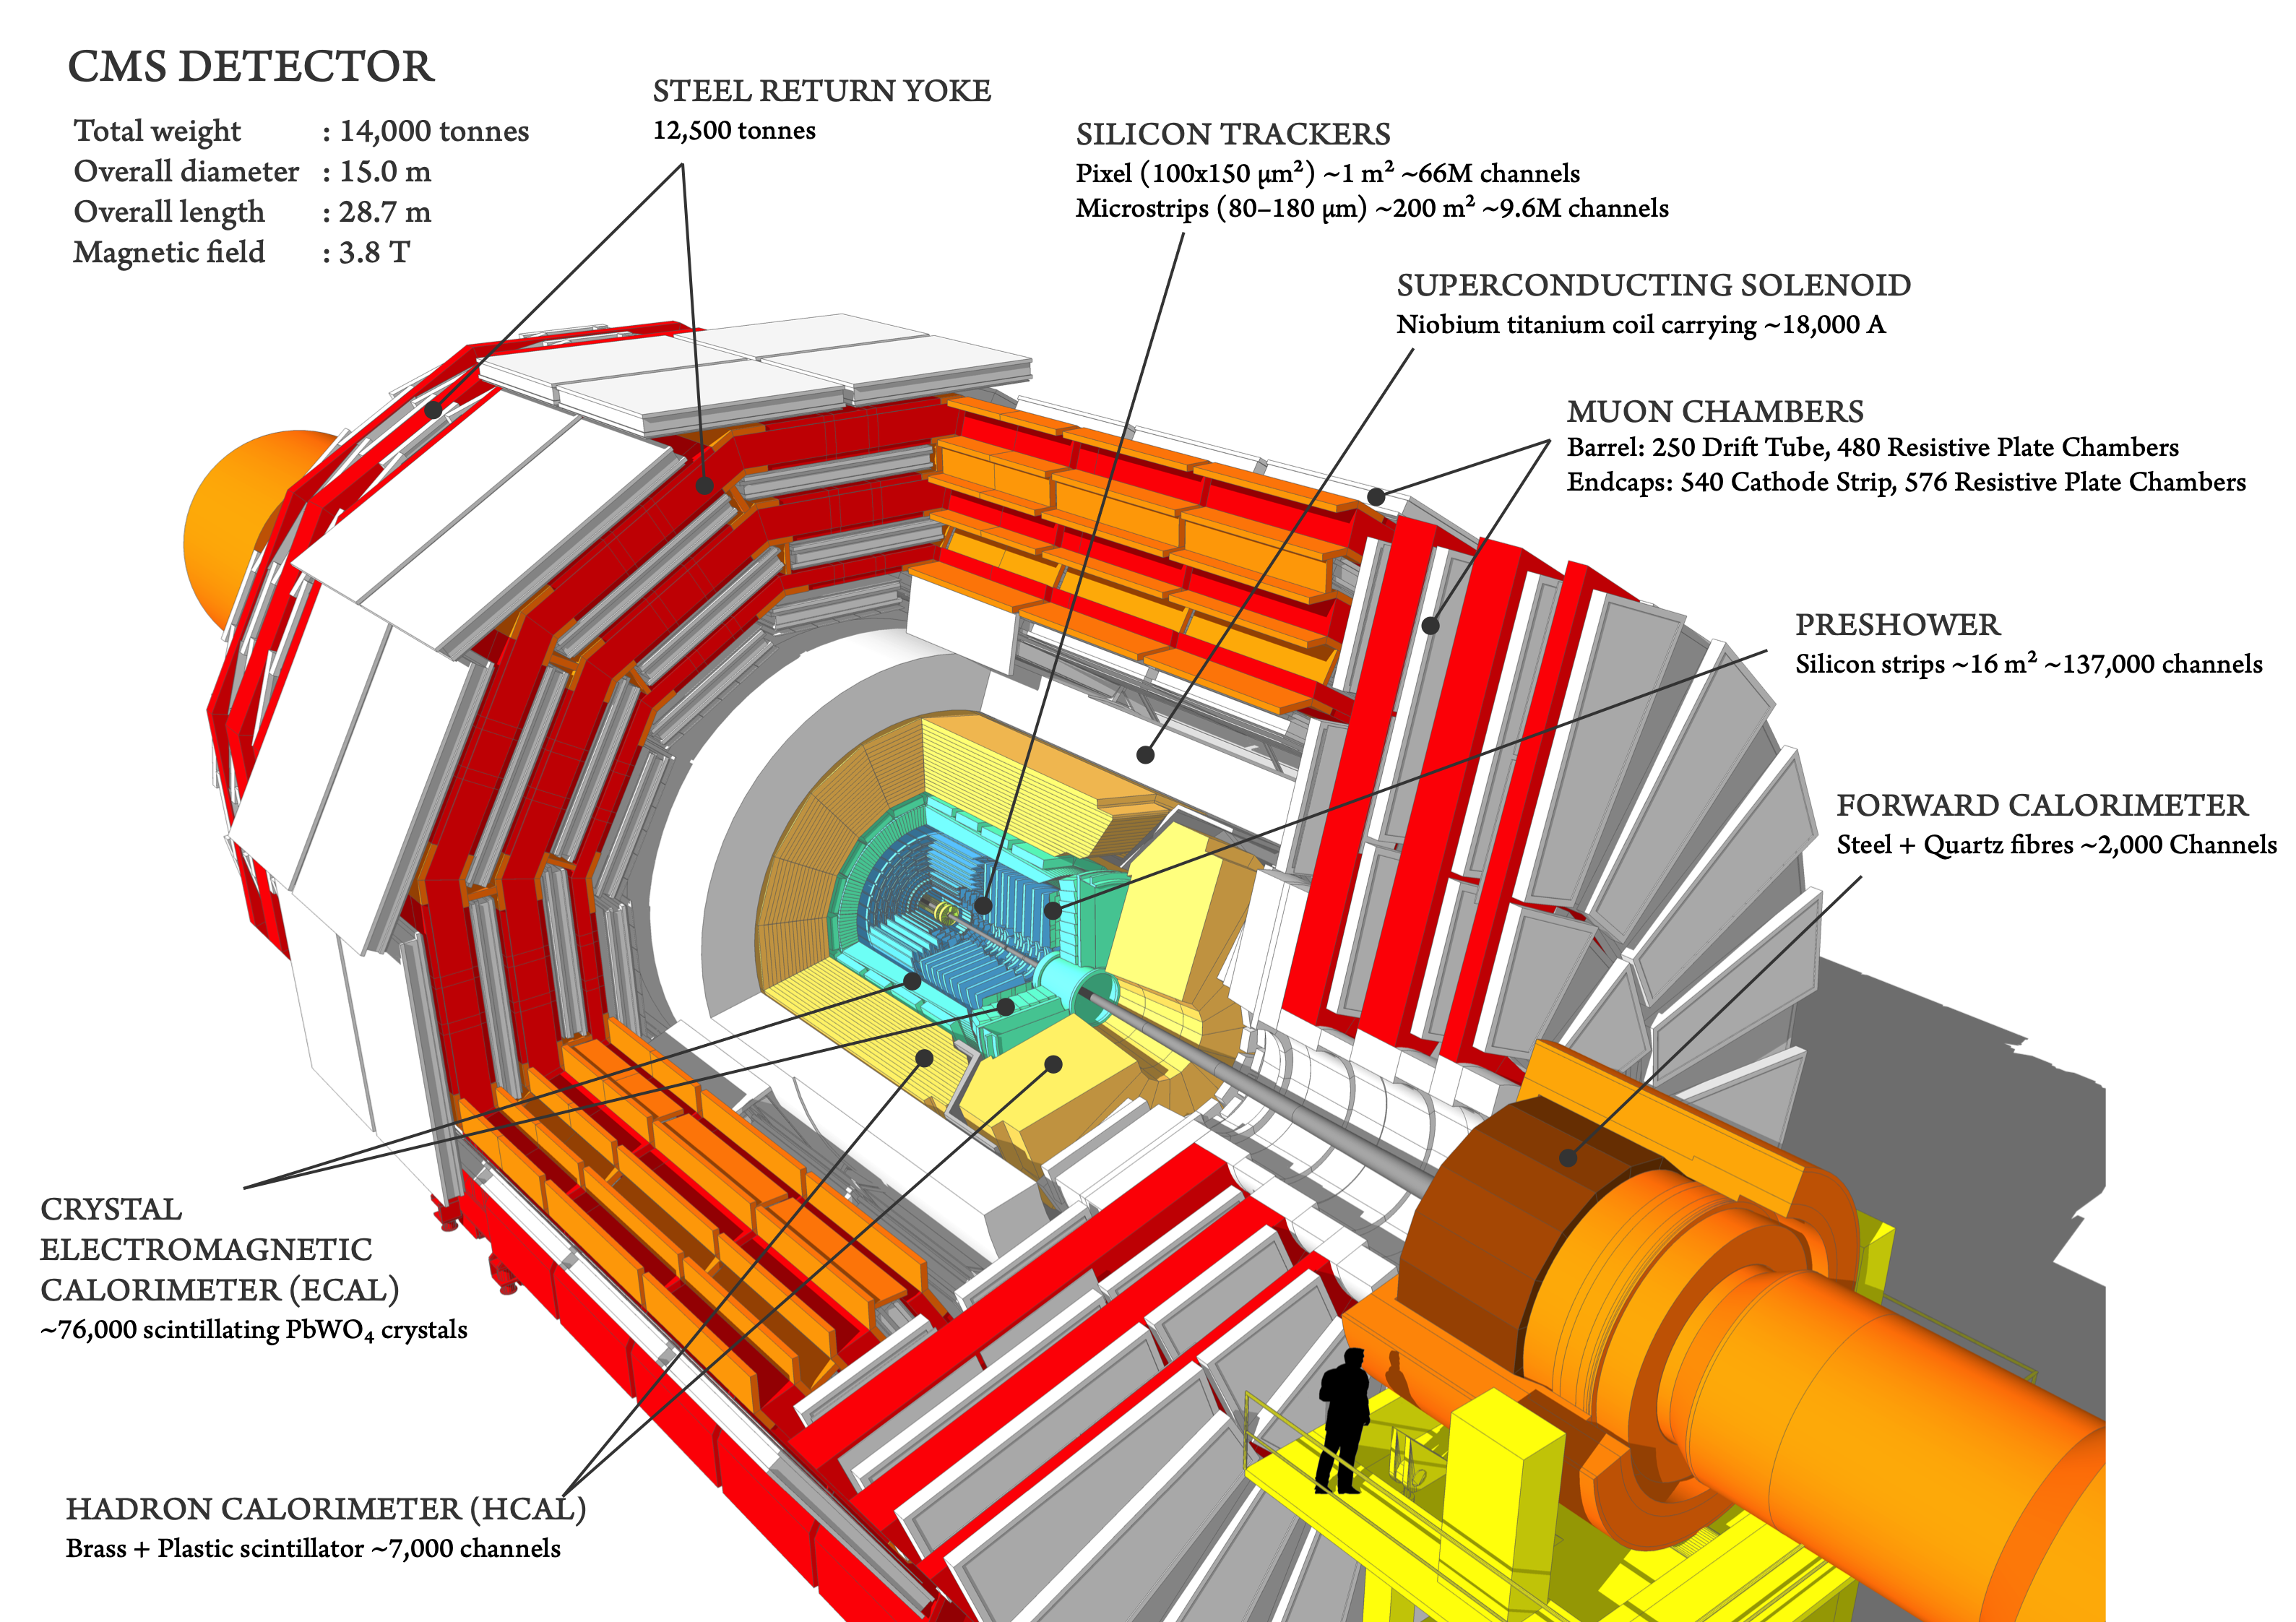
\includegraphics[width=0.9\hsize]{figures/cms_diagram.png}}
\legend{Schematic of the CMS detector showing its components.}
\source{\cite{Sakuma:2665537}}
\end{figure}

As the name implies, it is designed to make accurate identification and measurement of the transverse momentum of muons, which are very important particles as they appear in many SM and BSM processes.

An important component of the detector is the powerful 6 meters diameter superconducting solenoid, that can provide a magnetic field of 3.8 T. Such a powerful field is important in the accurate transverse momentum measurement with the bending of the trajectories of the particles.

From the innermost part, the subdetector systems that compose the CMS detector are: the tracker composed by the silicon pixel and strip tracker, the electromagnetic calorimeter (ECAL), the hadronic calorimeter (HCAL) and the Muon system.

\subsection{CMS Coordinate system}

The CMS coordinate system is pictured in the Figure \ref{fig:cms_coordinates}, it is a right-handed coordinate system centered in the nominal interaction point. The x-axis points out to the center of the LHC ring, the y-axis points upwards and the z-axis follows the anticlockwise beam pointing to the Jura Mountains, in France. The azimuthal angle is measured between the x-axis and the xy-plane and the $\theta$ angle is measured between the positive z-axis and the positive y-axis.

\tdplotsetmaincoords{75}{50} % to reset previous setting

\begin{figure}[!htm]{15cm} 
\caption{CMS Coordinate System}%
\label{fig:cms_coordinates}
\fbox{
    \begin{tikzpicture}[scale=2.7,tdplot_main_coords,rotate around x=90]
     
      % variables
      \def\rvec{1.2}
      \def\thetavec{40}
      \def\phivec{70}
      \def\R{1.1}
      \def\w{0.3}
     
      % axes
      \coordinate (O) at (0,0,0);
      \draw[thick,->] (0,0,0) -- (1,0,0) node[below left]{$x$};
      \draw[thick,->] (0,0,0) -- (0,1,0) node[below right]{$y$};
      \draw[thick,->] (0,0,0) -- (0,0,1) node[below right]{$z$};
      \tdplotsetcoord{P}{\rvec}{\thetavec}{\phivec}
     
      % vectors
      \draw[->,red] (O) -- (P) node[above left] {$P$};
      \draw[dashed,red] (O)  -- (Pxy);
      \draw[dashed,red] (P)  -- (Pxy);
      \draw[dashed,red] (Py) -- (Pxy);
     
      % circle - LHC
      \tdplotdrawarc[thick,rotate around x=90,black!70!blue]{(\R,0,0)}{\R}{0}{360}{}{}
     
      % compass - the line between CMS and ATLAS has a ~12° declination (http://googlecompass.com)
      \begin{scope}[shift={(1.1*\R,0,1.65*\R)},rotate around y=12]
        \draw[<->,black!50] (-\w,0,0) -- (\w,0,0);
        \draw[<->,black!50] (0,0,-\w) -- (0,0,\w);
        \node[above left,black!50,scale=0.6] at (-\w,0,0) {N};
      \end{scope}
     
      % nodes
      \node[left,align=center] at (0,0,1.1) {Jura};
      \node[right] at (\R,0,0) {LHC};
      \fill[radius=0.8pt,black!20!red]
        (O) circle node[left=4pt,below=2pt] {CMS};
      \draw[thick] (0.02,0,0) -- (0.5,0,0); % partially overdraw x-axis and CMS point
      \fill[radius=0.8pt,black!20!blue]
        (2*\R,0,0) circle
        node[right=4pt,below=2pt,scale=0.9] {ATLAS};
      \fill[radius=0.8pt,black!10!orange]
        ({\R*sqrt(2)/2+\R},0,{ \R*sqrt(2)/2}) circle % 45 degrees from ATLAS
        node[left=2pt,below=2pt,scale=0.8] {ALICE};
      \fill[radius=0.8pt,black!60!green]
        ({\R*sqrt(2)/2+\R},0,{-\R*sqrt(2)/2}) circle % 45 degrees from ATLAS
        node[below=2pt,right=2pt,scale=0.8] {LHCb};
     
      % arcs
      \tdplotdrawarc[->]{(O)}{0.2}{0}{\phivec}
        {above=2pt,right=-1pt,anchor=mid west}{$\phi$}
      \tdplotdrawarc[->,rotate around z=\phivec-90,rotate around y=-90]{(0,0,0)}{0.5}{0}{\thetavec}
        {anchor=mid east}{$\theta$}
    \end{tikzpicture}
}
\legend{Diagram of the CMS coordinate system. The coordinates are centred in the IP.}
\source{https://wiki.physik.uzh.ch/cms/latex:tikz}
\end{figure}

For the physics analysis, the momentum is one of the key variables of the particle as normally the theory is described in momentum space ($p_x, p_y, p_z$). The detector measures the momentum in terms of the transverse momentum ($p_T$), pseudorapidity ($\eta$), and the azimuthal angle ($\phi$). The $p_T$ is defined as:
\begin{equation}
    p_T = \sqrt{p_x^2 + p_y^2},
\end{equation}
the $\eta$ is an approximation to another variable, the rapidity (y), which is invariant by Lorentz boosts in the z-axis. With respect to the beam axis, the rapidity can be written as:
\begin{equation}
    y = \frac{1}{2} \ln{\left( \frac{E + p_z}{E - p_z} \right)}.
\end{equation}
But from the detector point of view it is a variable hard to be measured, as it depends on the energy of the particle. The pseudorapidity is a much more straightforward measurement as it is defined as
\begin{equation}
    \eta = - \ln {\left[ \tan{\left( \frac{\theta}{2} \right)} \right]},
\end{equation}
depending only on the $\theta$ angle. Furthermore, $\eta \approx y$ providing that the energy of the particle is much greater than its mass.

\subsection{Tracker}

The tracker is the detector closest to the IP, it is responsible to measure accurately the momentum of the charged particles and vertices positions. It is divided into two types of detectors, the Pixel tracker and the Silicon Strip tracker. Together, they provide a coverage of $|\eta| < 2.5$. A layout of the tracker detector is shown in Fig. \ref{fig:tracker_layout}

\begin{figure}[!htm]{15cm} 
\caption{CMS Tracker Detector Schematic}%
\label{fig:tracker_layout}
\fbox{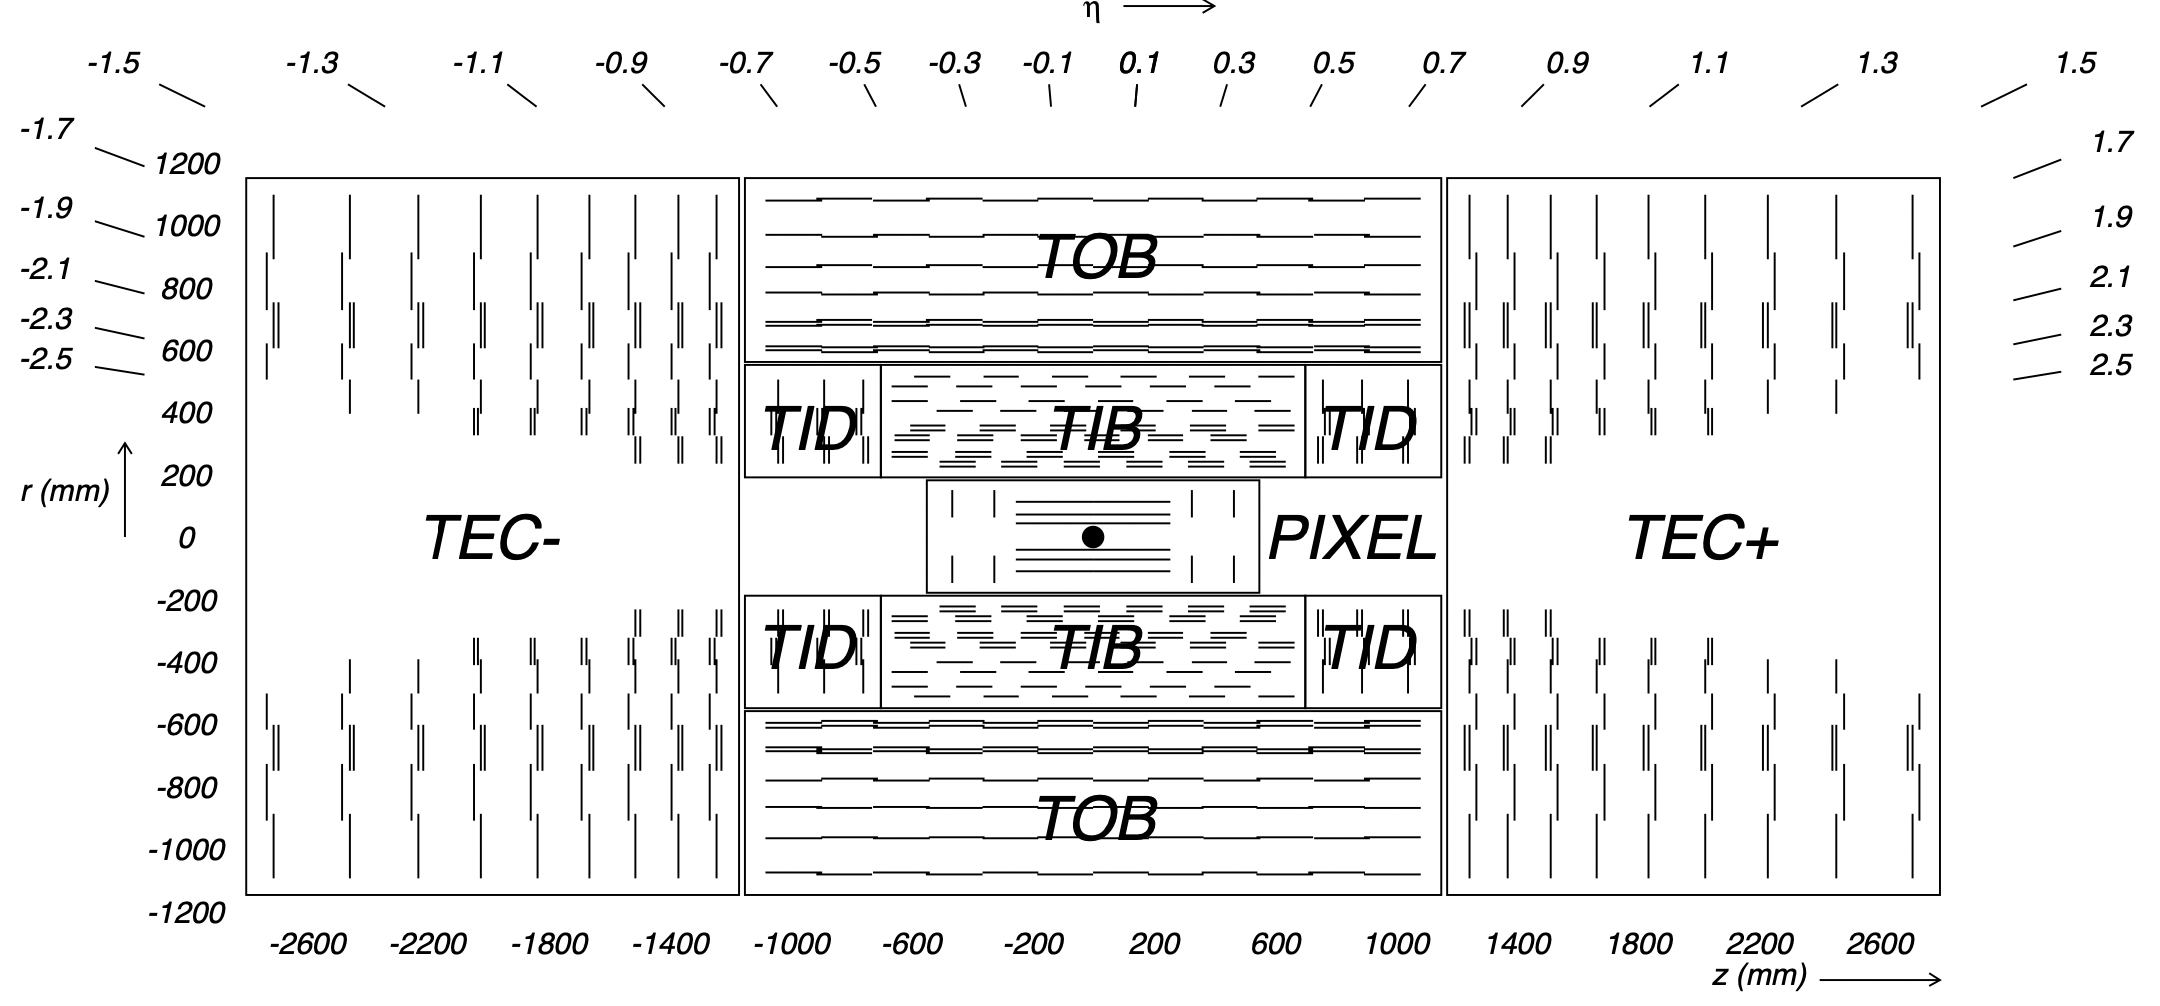
\includegraphics[width=0.9\hsize]{figures/tracker_detector.png}}
\legend{Schematic of a cross section of the tracker detector. }
\source{\cite{CMS:2008xjf}}
\end{figure}

The pixel detector consisted of three layers in the barrel and two layers in each endcap. After Phase-1\footnote{Phase-1 upgrade happened in the Technical Stop between 2016 and 2017} upgrade, an additional layer was added to the barrel and to each endcap as well as new readout system to minimize data losses and radiation degradation \cite{Dominguez:1481838}. The layout of the tracker before and after the Phase-1 upgrade is in Figure \ref{fig:pixel_layout}.

\begin{figure}[!htm]{15cm}
\caption{CMS Pixel Tracker Detector Layout}%
\label{fig:pixel_layout}
\fbox{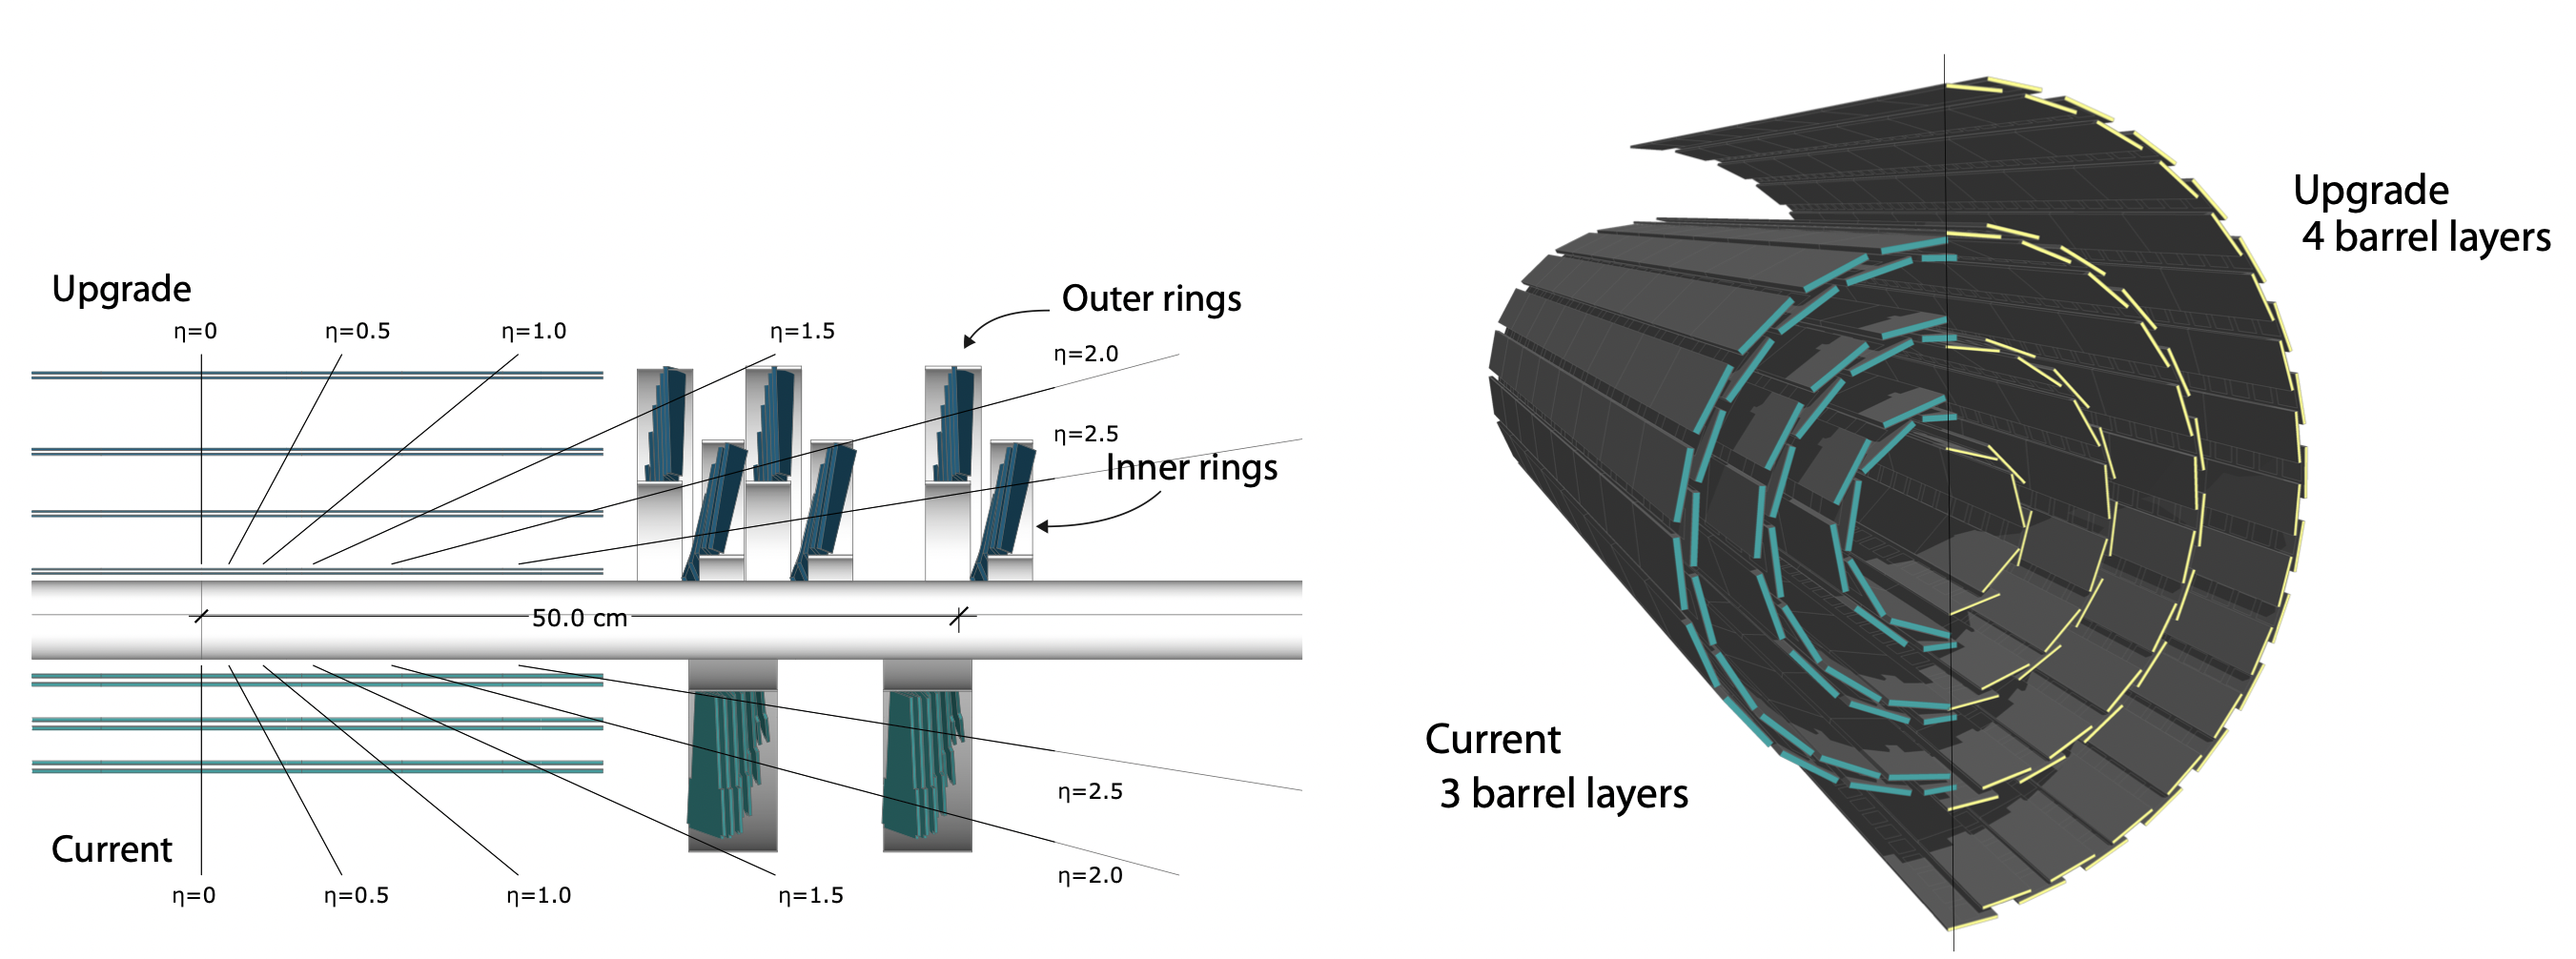
\includegraphics[width=0.9\hsize]{figures/pixel_layout.png}}
\legend{The layout of the CMS Pixel tracker detector before (labeled as current) and after the upgrade.}
\source{\cite{Dominguez:1481838}}
\end{figure}

The Silicon Strip detector is in the outer tracker region and consists of silicon micro-strips distributed in 198 $m^2$. It has ten layers in the barrel region and 3 layers in each endcap. It is divided in Tracker Inner Barrel (TIB), covering the central part of the detector, the Tracker Inner Disks (TID) at the inner endcap, both are surrounded by the Tracker Outer Barrel (TOB) on the barrel, and the Tracker Endcap (TEC).

\subsection{Electromagnetic Calorimeter}

The Electromagnetic Calorimeter (ECAL) is the responsible to measure the energy of photons and electrons, so it is designed to absorb these particles. It is done by interactions that occur in the lead tungstate ($PbWO_4$) crystals. A number of 61\,200 crystals are placed in the barrel (ECAL Barrel, EB) and 7\,324 in each endcap (ECAL Endcap, EE), amounting in a total of 75\,848 crystals, which coupled with to photodetectors, with output proportional to the energy left by the particle into the crystal. 

Also, in front of the endcap detector there is a Preshower detector that is composed of two layers of silicon detectors interleaved by a lead radiator. They were designed to identify the neutral pions decay into two photons and separate them from the primary photons.

Its coverage is $|\eta| < 1.48$ in the barrel region (EB) and  $1.48 < |\eta| < 3.0$ in the endcap region (EE). The Figure \ref{fig:ecal_layout} shows a layout of the ECAL.

\begin{figure}[!htm]{15cm} 
\caption{CMS Electromagnetic Calorimeter layout}%
\label{fig:ecal_layout}
\fbox{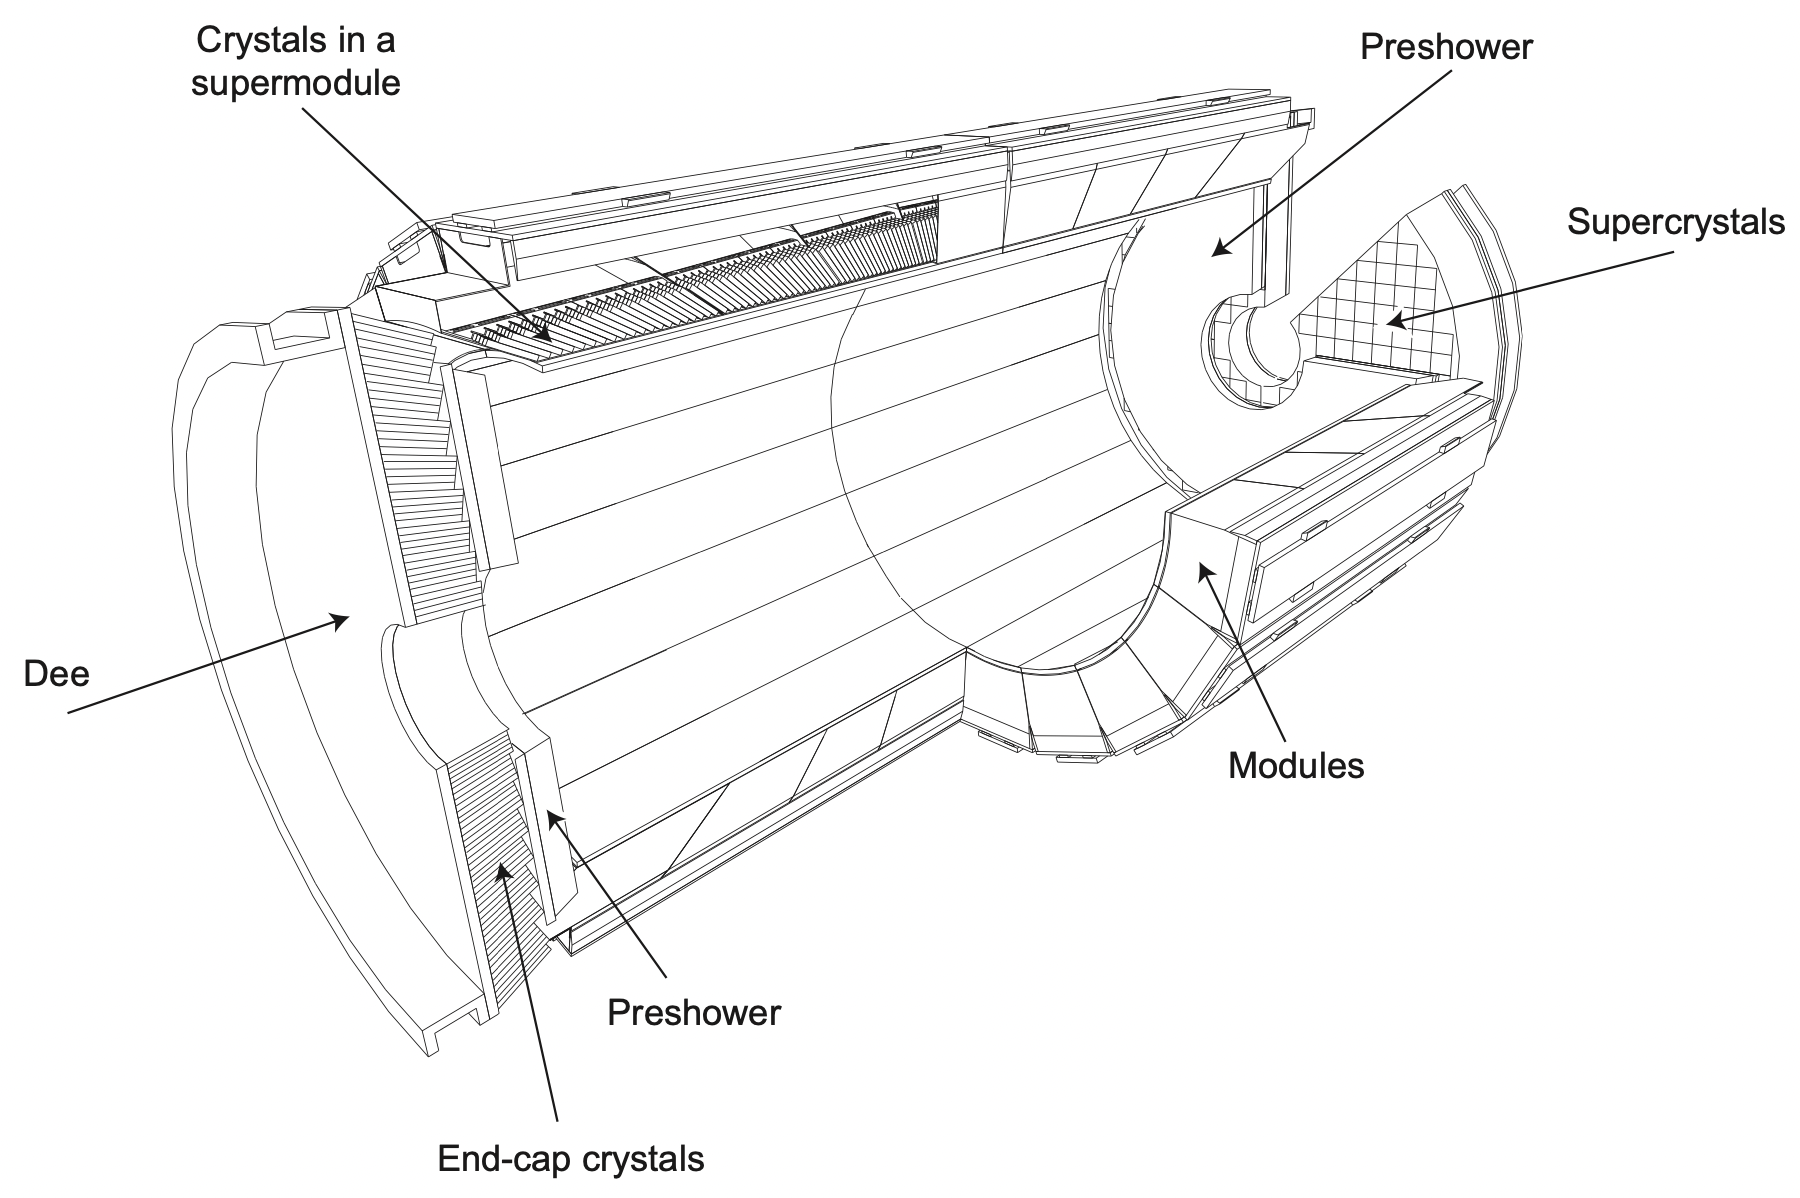
\includegraphics[width=0.7\hsize]{figures/ECAL_layout.png}}
\legend{Layout of CMS electromagnetic calorimeter, showing its components.}
\source{\cite{CMS:2008xjf}}
\end{figure}

\subsection{Hadronic Calorimeter}

The Hadronic Calorimeter (HCAL) is the responsible to measure energy of the charged and neutral hadrons, being very important for jet and missing energy measurement. It covers an extended pseudorapidity region ($|\eta| < 5.2$) to enhance the missing transverse energy estimation.

It is made of layers of steel and brass alternated with very thin plastic scintillator tiles, in order to maximize the amount of absorptive material, allowing for hadronic cascades.

The HCAL is divided into four regions, the HCAL Barrel (HB) surrounded by the superconducting solenoid covering $|\eta| < 1.4$, the Outer Calorimeter (HO) outside of the solenoid, it is placed there to identify late starting showers, it covers $|\eta| < 1.26$, the HCAL Endcaps (HE), covering $1.2 < |\eta| < 3.0$ and Forward Calorimeters (HF) $3.0 < |\eta| < 5.2$ and located at 11.2 m of the interaction point. The HF uses quartz fibers instead of brass, which provide Cherenkov light detection. Figure \ref{fig:hcal_layout} shows a layout of the HCAL.

\begin{figure}[!htm]{15cm} 
\caption{Longitudinal View of CMS Hadronic Calorimeter}%
\label{fig:hcal_layout}
\fbox{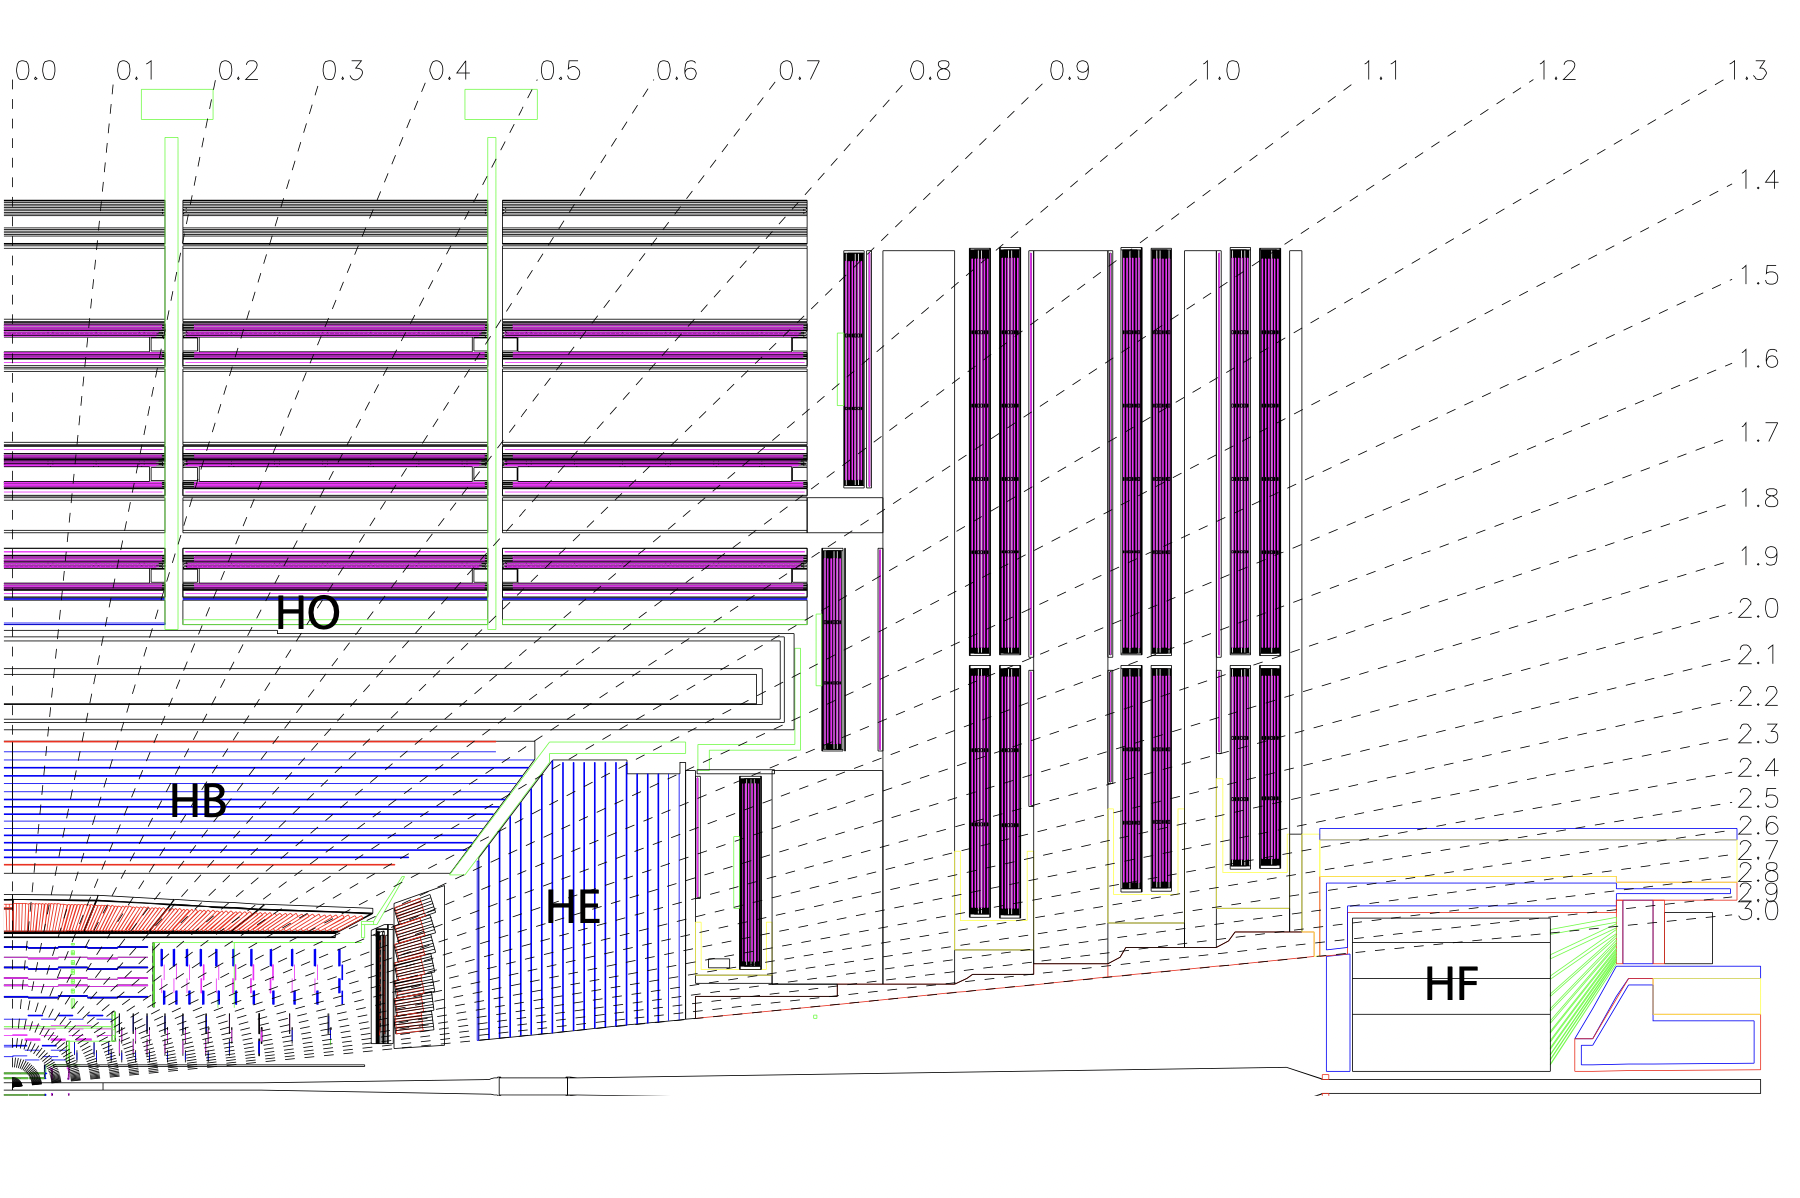
\includegraphics[width=0.9\hsize]{figures/HCAL_view.png}}
\legend{Longitudinal view of CMS hadronic calorimeter, showing its regions: HCAL Barrel (HB), Outer Calorimeter (HO), HCAL Endcaps (HE) and Forward Calorimeters (HF).}
\source{\cite{CMS:2008xjf}}
\end{figure}

\subsection{Muon Detector}

The CMS detector features a very powerful muon detection system located in the most outward region of the detector. The muons played a significant contribution to many of the physics results of CMS including the Higgs discovery\footnote{One of the first measured Higgs decay channel features four final state leptons $H \rightarrow ZZ \rightarrow 4 l$.}. The goals of the Muon System are to identify, measure momentum and provide triggering for the muons. Figure \ref{fig:cms_muon} shows a quadrant view of the Muon System highlighting also chambers that will be installed during the Phase-2 upgrade.

\begin{figure}[!htm]{15cm}
\caption{Quadrant View of the CMS Muon System}%
\label{fig:cms_muon}
\fbox{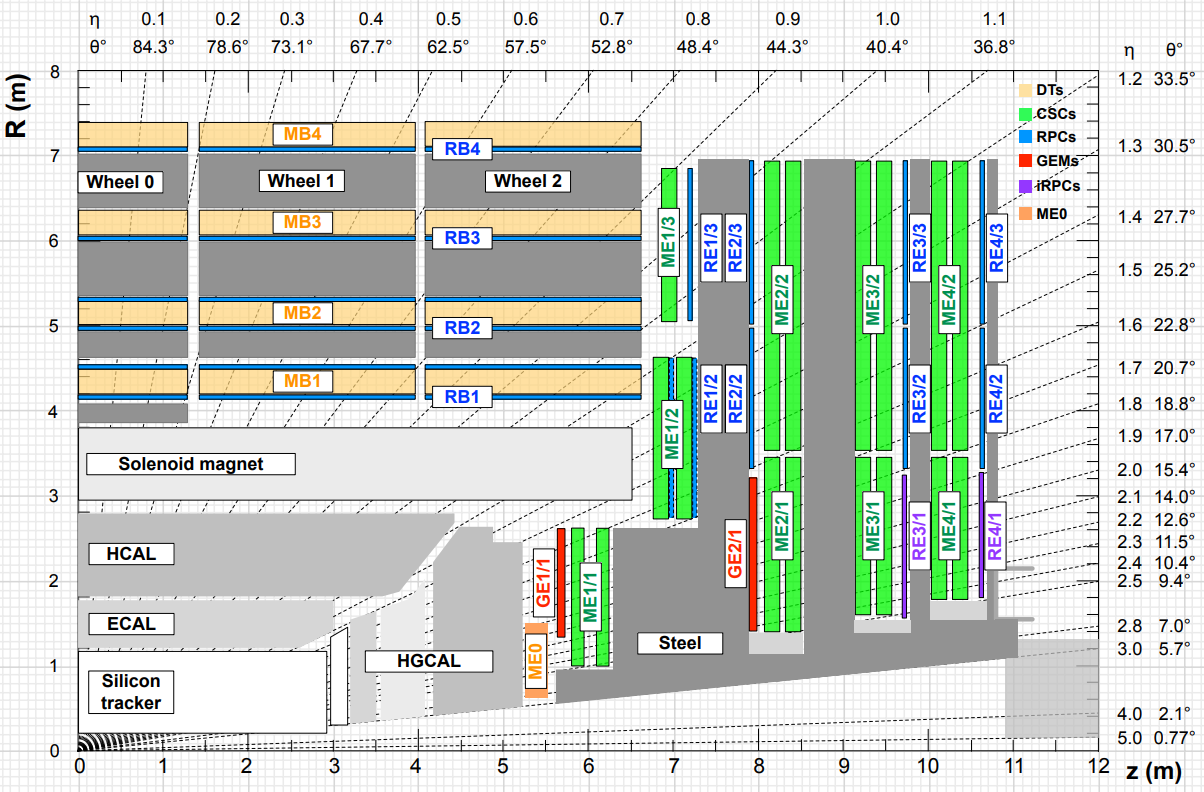
\includegraphics[width=0.9\hsize]{figures/muon_system.png}}
\legend{A quadrant view of the CMS detector highlighting its muon system after the phase-2 upgrade (RE3/1, RE4/1, GE1/1, GE2/1, ME0). DTs are coloured in yellow, CSCs in Green, RPCs in blue and GEMs in red and in orange. During LS2 the chambers GE1/1 were installed and are participating in Run 3}
\source{\cite{CERN-LHCC-2017-012}}
\end{figure}

The Muon System is composed of 4 different gaseous detector technologies:
\begin{itemize}
    \item \textbf{Drift Tubes (DT):} Have a gas mixture composed of 85\% $Ar$ and 15\% $CO_2$. The DT are located in the barrel ($|\eta| < 1.2$) providing spatial measurements for offline tracking, because of the fine spatial resolution of 100 $\mu m$, and trigger information. It is composed of 205 chambers divided in 12 sectors in $\phi$ and 5 wheels (longitudinal sections). 
    \item \textbf{Cathode Strip Chambers (CSC):} Located in the endcap ($0.9 < |\eta| < 2.4$), the CSC subsystem is composed of 540 chambers which provide triggering and position measurements, with a spatial resolution ranging from 50 to 140 $\mu$m. The gas mixture is composed of 50\% $CO_2$, 40\% $Ar$, and 10\% $CF_4$. 
    \item \textbf{Resistive plate Chambers (RPC):} Located in both regions, barrel and endcap, covering $|\eta| < 1.9$. It is used mainly for triggering, due to its timing capabilities. The CMS RPC system will be better discussed in the chapter \ref{chap:rpc}.
    \item \textbf{Gas-Electron Multiplier (GEM):} The GEMs were installed after Run 2, during the LHC Long-Shutdown period (LS2). They have both, good spatial and time resolution, complementing the CSCs high particle rate forward region ($ 1.6 < |\eta| < 2.2$).
\end{itemize}

\subsection{Trigger and Data Acquisition}

The proton-proton collision rate in LHC is extremely high, the bunch crossing (BX) frequency is 40 MHz and in each one of them many collisions can happen. It would be impossible to store and process this amount of events. To cope with these numbers, CMS uses a two tiered trigger to reduce the event rate to about 1 kHz.

First the event passes through a first level trigger called L1, which uses custom hardware processors information directly from the calorimeters and the muon detectors, to reduce the event rate to around 100 kHz. The L1 trigger relies on the transferring the data in optical links and processing it using FPGAs (Field Programmable Gate Arrays) to deliver the maximum readout speed and minimum latency \cite{CMS:2020cmk}.

The High Level Trigger (HLT) further processes the events accepted by the L1, doing more refined analysis on the events, which includes particle tracking. This trigger tier is centred in the concept of HLT path, which is a structured set of algorithms that selects the events. Those are simplified versions of the offline reconstruction algorithms, which run in a computing farm. Finally, the HLT chooses the data to be stored, by putting together the selected events accepted by a collection of HLT paths, forming a trigger menu.

\subsection{The Particle Flow Algorithm}

All the events accepted by the HLT are recorded and processed in the offline analysis in order to build the physics objects\footnote{Such as muons, electrons, photons, jets, missing transverse energy, etc.}. The physics objects are reconstructed from the input from all the different subdetectors using an algorithm called Particle Flow (PF) \cite{CMS:2017yfk}.

The particles originating from the collisions leave signals in the detectors starting by the tracker, in which charged particles leave signals (hits) that serve as input to find their trajectories (tracks) and origin point (vertices). The magnetic field bends the charged particles' tracks, making it possible to determine their momentum. Electrons and photons are absorbed by the electromagnetic calorimeter (ECAL), creating electromagnetic showers, and making it possible to measure their direction and energy. Charged and neutral hadrons initiate a hadronic shower, which is fully absorbed by the hadron calorimeter (HCAL), so that their direction and energy can be estimated. Muons and neutrinos travel through the calorimeters with almost no interaction. Muons produce additional hits in the muon system. Neutrinos pass undetected, so a missing energy can be attributed to its presence in the event. The Figure \ref{fig:pf_cms} shows the signals left in the detector by different particles.

\begin{figure}[!htm]{15cm}
\caption{Particle interactions in the parts of the CMS detector}%
\label{fig:pf_cms}
\fbox{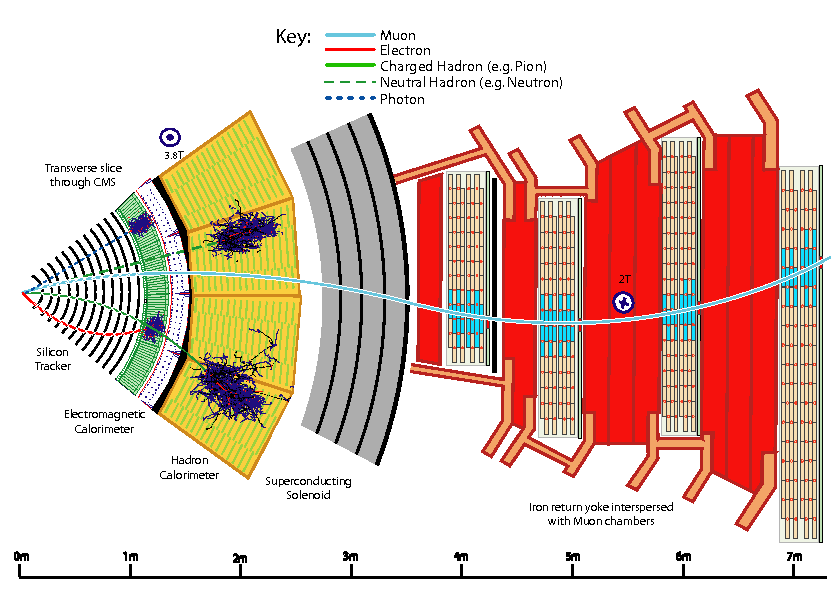
\includegraphics[width=0.9\hsize]{figures/pf_cms.png}}
\legend{A drawing of the different particle interactions occurring in the CMS detector.}
\source{\cite{CMS:2017yfk}.}
\end{figure}

The Particle Flow was first used in the ALEPH detector, at LEP \cite{ALEPH:1994ayc}. A very important requirement is a fine spatial granularity of the detector layers, since a course granularity can make signal from different objects to be merged, reducing the reconstruction and identification capabilities.

The CMS is well suited for the PF because: the high magnetic field separates the jet's charged and neutral hadrons energy deposits in the calorimeters, the fine grained tracker can provide a pure and efficient charged-particle trajectory reconstruction in jets with transverse momentum up to around 1 TeV, a highly segmented ECAL allows a very good separation of energy clusters from different particles, a course segmented HCAL, which can still separate the charged and neutral hadrons clusters, and very good muon system which provide muon identification.
\chapter{The CMS Resistive Plate Chambers}\label{chap:rpc}
%================================================================

This chapter will discuss about on the CMS RPC system, where the author was able to work. A brief history of gaseous detectors will be presented, with focus on the RPC detector. The CMS RPC project will be introduced and the work my contributions will be presented.

\section{Brief history of gaseous detectors}

The first gaseous detector was introduced by E. Rutherford and H. Geiger in 1908 \cite{rutherford1908electrical}. The device consisted in a thin wire, the anode, coaxial to a cylindrical cathode filled with gas. When a ionizing particle passed through the gas, it ionized the gas particles. By applying a difference of potential to the device, the released electrons accelerate to the anode and inelastic collisions with other molecules multiplying the effect of the ionization in the so-called avalanche process, which was studied by John Sealy Townsend, between 1897 to 1901 \cite{peskov2018resistive}. An illustration of the avalanche formation in gaseous detectors is shown in Fig. \ref{fig:avalanche}. This kind of detector is still used up to today, mainly on radiation detection and monitoring.

\begin{figure}[!htm]{15cm}
\caption{Avalanche formation in gaseous detectors}%
\label{fig:avalanche}
\fbox{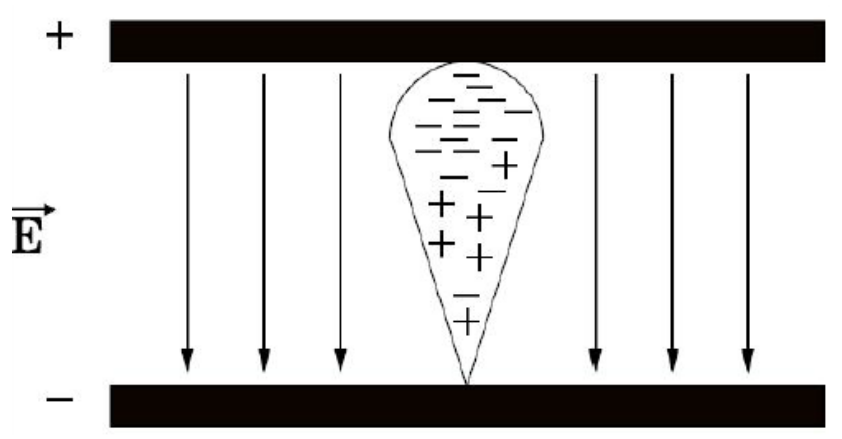
\includegraphics[width=0.5\hsize]{figures/avalanche_formation.png}}
\legend{The formation of a avalanche in gaseous detectors. The ionised electrons drift towards the anode because of the external electric field. As they accelerate, new electrons-ion pairs are formed multiplying the initial ionisation. The drop-like shape of the avalanche is caused by the difference in the drift velocity of electrons and ions.}
\source{\cite{Shopova:2626243}}
\end{figure}

This device operation depends on the applied voltage as shown Fig. \ref{fig:gaseous_curve}. At lower electric field strength, the electron and ions drifts with no avalanche multiplication and the number of electron-ion pairs is independent of of the voltage, at the ionization chamber mode. At the proportional mode the avalanche process occurs for each ionization, so that the number of electron-ion pairs is proportional to the energy deposited by the ionizing particle in the detector. Finally, at even higher voltage, in the Geiger-Müller counter region, there is emission of UV photons creating multiple avalanches along the anode wire \cite{o1961detection}. Also, at higher voltage levels the avalanches can increase into streamers, and even to sparks.

\begin{figure}[!htm]{15cm} 
\caption{Gaseous Counter Characteristic Curve}%
\label{fig:gaseous_curve}
\fbox{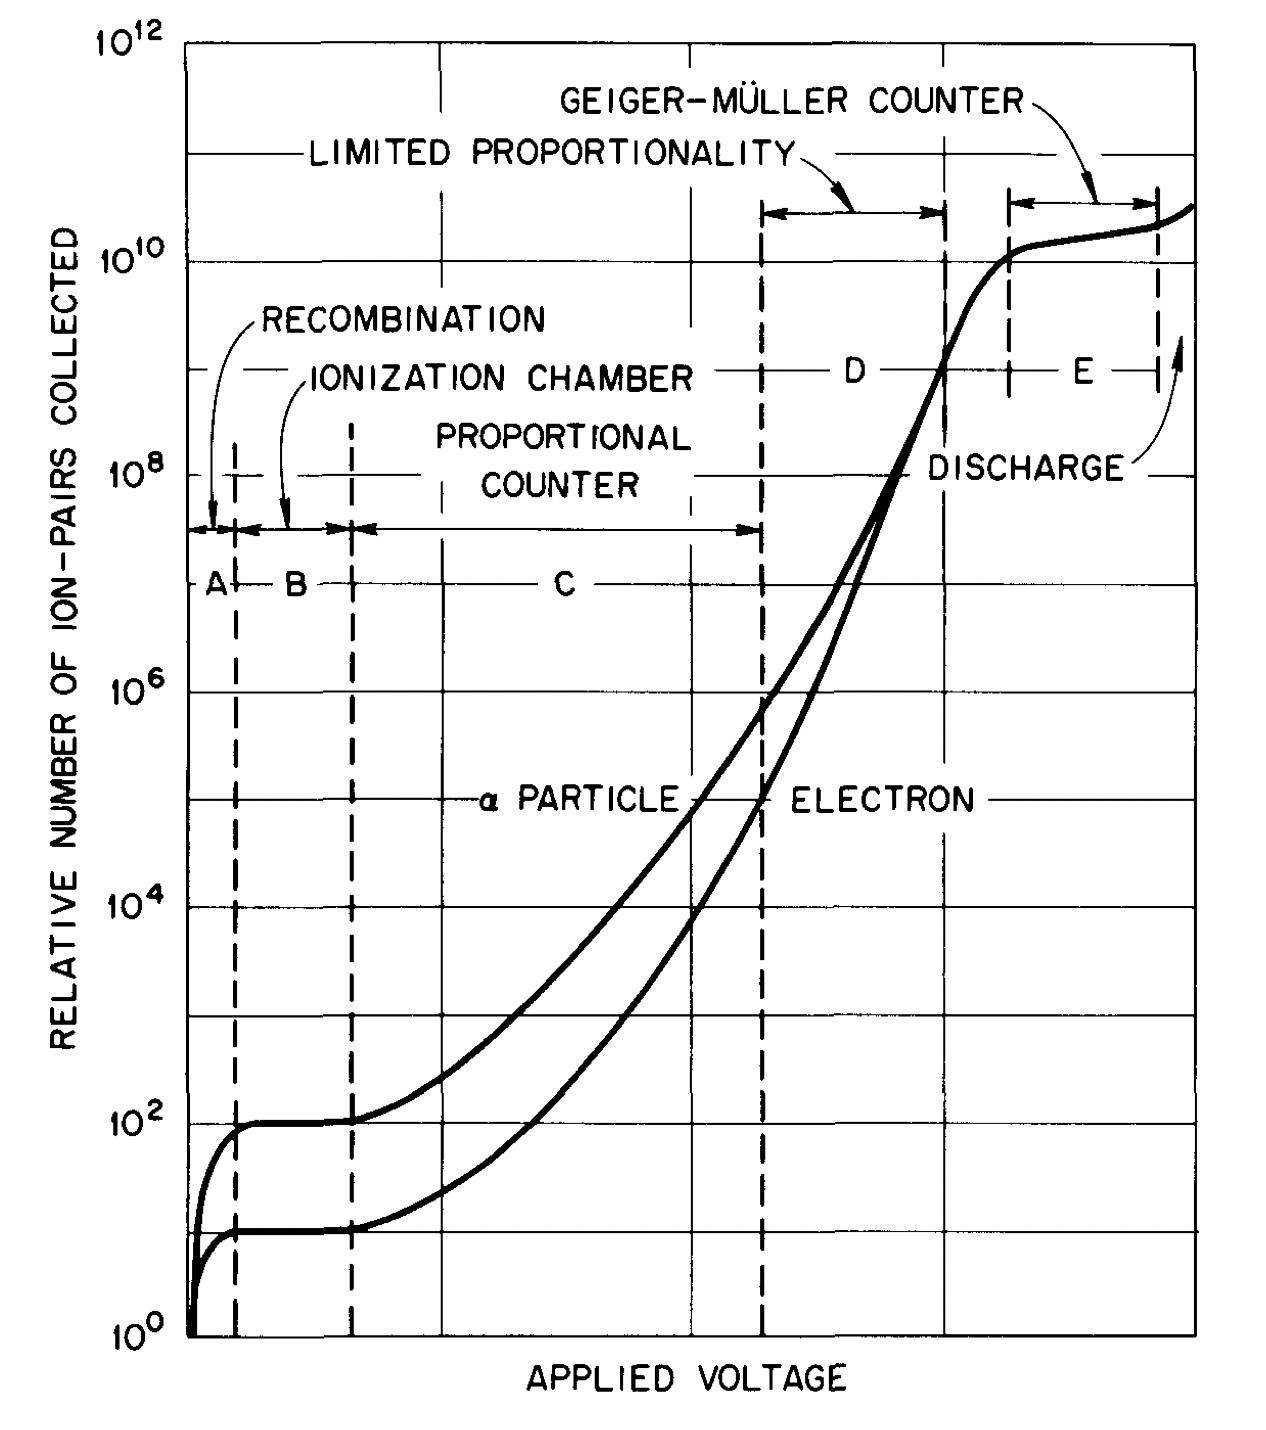
\includegraphics[width=0.5\hsize]{figures/gaseous_detector_curve.png}}
\legend{Curve of the relative number of ion pairs collected in a gaseous counter as a function of the applied voltage.}
\source{\cite{o1961detection}}
\end{figure}

But this devices are not suitable for the use in high-energy particle physics tracking. From the 1930s to the 1960s, the research was mainly done using cloud chambers as bubble chambers, which have excellent imaging capabilities, with the major drawback of being active during a selected time interval, being unsuitable to analysis of rare events \cite{sauli2015gaseous}.

The first gaseous detector to be able to have an very good tracking capability was the spark chambers \cite{fukui1959new}. On this one, rather than a constant voltage applied to its terminals, they had a pulse voltage applied to a parallel-plate gap shortly after the detection of a coincidence signal from scintillation detectors. A visible track would grow from the ionization trail left in the gas. Combined to a photography readout, they became great assets to the particle detection, with a major drawback, the slow rates they could operate on, around dozens of Hertz \cite{sauli2015gaseous}.

In 1968, Georges Charpak created the multiwire proportional chamber (MWPC) \cite{Charpak:1968kd}. A schematic of a MWPC is shown in Fig. \ref{fig:MWPCsch}. It had a fast electronic readout, capable of withstanding high rates, had excellent time and space resolutions and was a continuously operating device. It was a major development in the particle detector field, the MWPCs and other detectors based on it\footnote{Such as drift chambers, time projection chambers, etc.} replaced other detectors with photographic readout. Still, a major drawback of such detectors was the time resolution, in the order of $\mu$s, because the drift time variate a lot depending on the position where the primary electron is created. 

\begin{figure}[!htm]{15cm}
\caption{Multiwire Proportional Chamber Schematic}%
\label{fig:MWPCsch}
\fbox{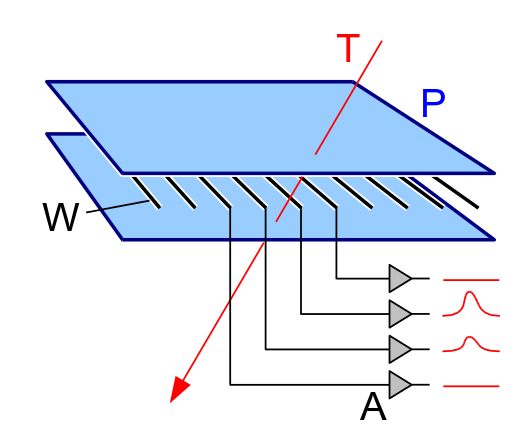
\includegraphics[width=0.5\hsize]{figures/Wire_chamber_schematic.png}}
\legend{A schematic of a multiwire proportinal chamber. The blue plates are the cathodes and the wires are the anodes. When the a particle ionises the gas, the electrons drift towards the wires and, because of the avalanche multiplication, many electron are collected and a measurable signal is obtained at the anodes.}
\source{\cite{wiki:wire}}
\end{figure}

Parallel-plate geometry detectors tend to perform better on this area, because the electric field is uniform, so that all the gas volume is available for amplification, providing excellent timing capabilities \cite{PARKHOMCHUCK1971269}. A successful implementation of the parallel-plate geometry are the resistive plate chambers.

\section{Resistive Plate Chambers}

The RPC was created in 1981 by Santonico and Cardarelli \cite{santonico1981development}. This detector is very similar to a spark chamber, but with a major difference, its electrodes are made of materials with high electrical resistivity, in the order of $10^{10}-10^{12} \; \Omega$cm, made with high pressure laminate (HPL), also known as Bakelite, or glass. The electrodes are coated with a conductive layer to provide good connection to the applied high voltage (HV). 

The two plates form a region where a mixture of gases is flushed, denominated gas gap. The thickness normally goes from 1-2 mm\footnote{Some designs have lower thickness, for instance, check \cite{Deppner:2016yku}} and it is maintained constant by a network of spacers distributed throughout the plane. The signal readout is independent of the HV, it can be performed by copper strips or pads where the avalanche induces signals. A typical design of a RPC chamber is shown in Fig. \ref{fig:RPC_schematic}.

\begin{figure}[!htm]{15cm}
\caption{Resistive Plate Chamber Schematic}%
\label{fig:RPC_schematic}
\fbox{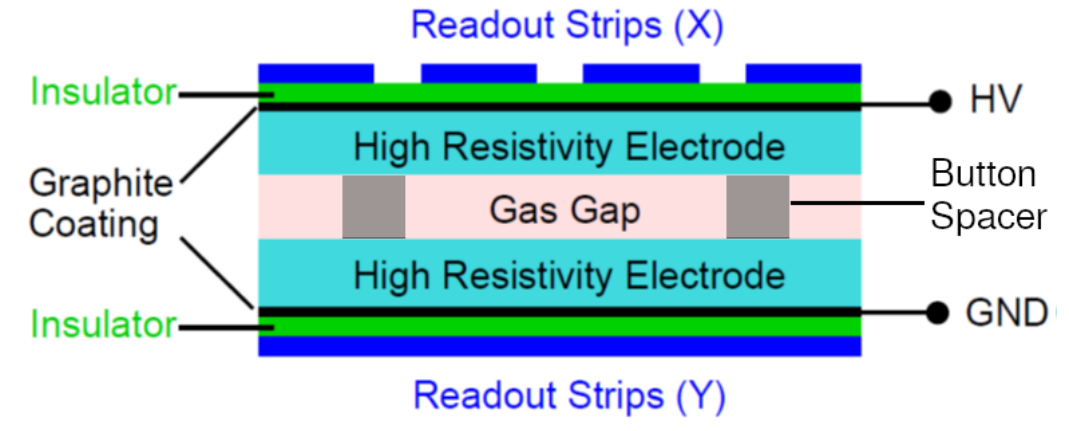
\includegraphics[width=0.5\hsize]{figures/RPC_schematic.png}}
\legend{A Schematic of a typical RPC with one gap and readout by strips in two directions}
\source{\cite{Mondal:2018eov}}
\end{figure}

The gas mixture is very important for efficient operation of the RPC. Normally, a mixture of tetrafluoroethane (C$_2$H$_2$F$_4$, commercially known as R134a or Freon) to enhance ionization of the incident particles, that can compose more than 90\% of the mixture, isobutane (iC$_4$H$_10$) as a quencher gas and (SF$_6$) to improve the electronegativity of the mixture and reduce the secondary ionization. Nowadays, the search of eco-friendly gas mixtures is very important research field for the RPCs. The replacement is very important for the R134a and SF$_6$ as they contribute the most to the high global warming potential (GWP) of the mixture. The commercial replacement to the R134a are the HydroFluoroOlefyns (HFOs), for example the HFO1234ze (C$_2$H$_2$F$_4$) which brings the HV working point (WP) of the RPCs to higher values. Normally, it is added CO$_2$ or Helium to the HFO to bring the WP to a lower level. For the SF$_6$ some gases are being researched, for example, 3M Novec 5110, 3M Novec 4710, AMOLEA HFO-1224yd, etc. More details on the eco gas research can be found in \cite{Guida:2022pyg}. Some alternatives to reduce the flushing of fresh gas into the system, such as gas re-circulation systems, are also being developed \cite{Corbetta:2020esl}.

The detector operates on a very high electrical field strength, in the order of 4-5 kV/mm. The authors of \cite{Santonico:1988qi} pointed out that, when a particle passes by the gas volume, the primary electron-ion pairs gives rise to a small discharge that is quenched without affecting the whole gas volume by the following mechanisms:
\begin{itemize}
    \item Reduction of the electric field in the electrode at the region close to the discharge development, due to the high resistivity electrodes;
    \item Absorption of the ultraviolet (UV) photons created in the discharge by the isobutane, preventing secondary discharges;
    \item Capture of the electrons in the outer region of the discharge because of the high electronegativity of the Freon.
\end{itemize}

Because of these mechanisms, the discharges in the RPC are not harmful, not destroying the chamber or the front-end electronics. Furthermore, the size of the region affected by the discharge is small, leaving the rest of the chamber active, so that it can sustain higher rates. Coupling these characteristics to the excellent time resolution (some designs in the order of 50 ps) good spatial resolution (up to 50 $\mu$m state of art designs \cite{Francke:2002wq}) and the relatively easy construction and cheap construction, the RPCs are very well suitable for high energy physics experiments, even for tracking. Normally, they are employed in muon systems, where it can cover an area of thousands of square meters as in the case of the CMS Experiment.

\section{CMS RPC Project}

The CMS RPC system consists in 1056 double-gap chambers operating in avalanche mode. Each gap is constructed with two HPL sheets of bulk resistivity 1-6 $\times 10^{10} \; \Omega$ cm. The HPL sheets are spaced 2 mm apart by a grid of plastic spacers. The internal surfaces of the gaps are coated with a 35 to 45 $\mu$m linseed oil. This treatment improves greatly the performance of the chambers, because it smooths the internal surfaces and quench UV photons \cite{Abbrescia:687074, Lu:2009zzd}. The outside surfaces are coated with a conductive graphite paint, forming the electrodes, and isolated by a PET film. One gap is placed on top of the other with a readout of copper strips placed in between. The layout of a double-gap RPC is shown in Figure \ref{fig:RPClayout}. Everything is placed inside a aluminum case.

\begin{figure}[!htm]{15cm}
\caption{Double-gap CMS RPC layout}%
\label{fig:RPClayout}
\fbox{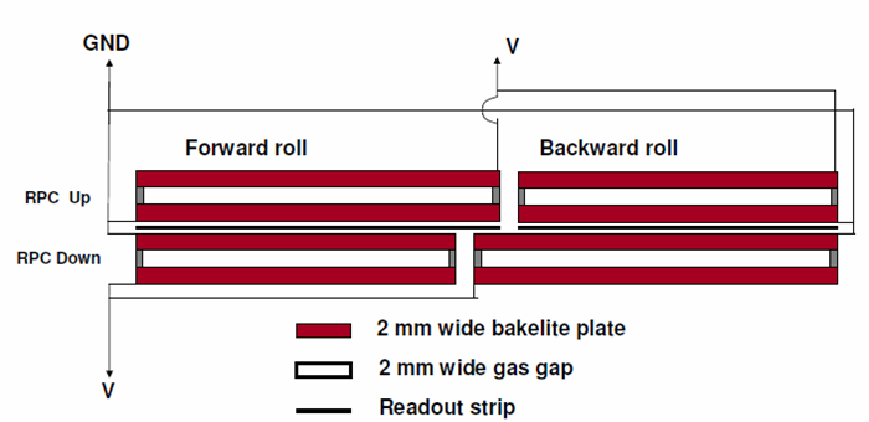
\includegraphics[width=0.5\hsize]{figures/RPC_layout.png}}
\legend{A schematic of a CMS RPC placed in the barrel region. }
\source{\cite{Costantini:1477020}}
\end{figure}

The gas mixture employed, named CMS RPC standard gas mixture, is composed of 95.2 \% of R134a, 4.5 \% of isobutane and 0.3 \% of SF$_6$ kept at 21 $^\circ$C with relative humidity of 40-50 \% to keep the bakelite resistivity stable. 

The RPC system is able to withstand high rate capability of the order of 300 Hz/cm$^2$ a have efficiency greater than 95 \%, cluster size\footnote{number of adjacent strips fired in a single muon hit} less than 2 for a better spatial resolution between 0.8-1.3 cm, the time resolution is 1.5 ns making them interesting for triggering and BX assignment. There are RPCs both in the barrel and the endcap regions of CMS covering an area of 3500 m$^2$. 

\section{CMS RPC Barrel}

In barrel, there are 480 chambers distributed in 5 wheels (Wheel $\pm$ 2, $\pm$ 1 and 0) along the beam pipe. Each wheel consists in 4 stations (RB1-RB4) along the radius. The two inner stations consists of two RPC chambers with a DT in the middle and the two outer stations have only one RPC and one DT. Also, the wheel is divided in 12 sectors (S01-S12) along the direction of the azimuthal angle $\phi$. Due to mechanical reasons, RB3 and RB4 are further divided into two chambers (named + and –) along $\phi$ in all sectors but S04, S09 and S11 in RB4. Since RB4/S09 and RB4/S11 are in the feet of the barrel wheel, they have a single RPC. RB4/S04 have four chambers (named --, -, + and ++). The RPC barrel is given in Figure \ref{fig:RPC_barrel_layout}.

\begin{figure}[!htm]{15cm}
\caption{CMS RPC barrel layout}%
\label{fig:RPC_barrel_layout}
\fbox{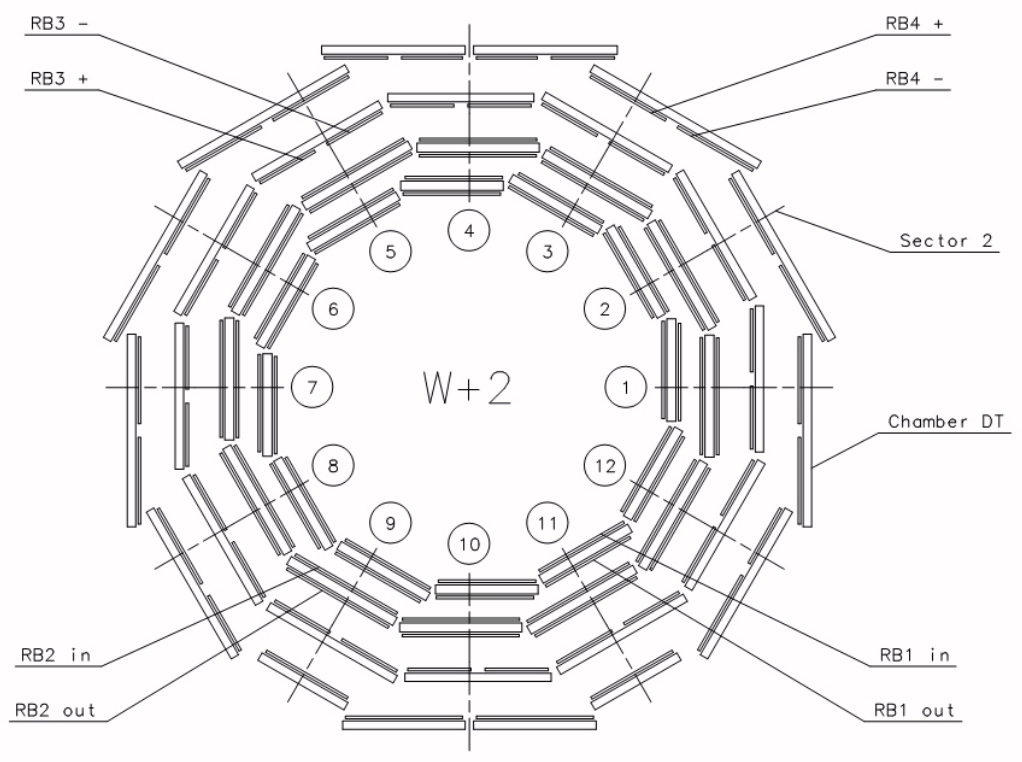
\includegraphics[width=.7\hsize]{figures/RPC_barrel_layout.png}}
\legend{Layout of RPCs placed in the CMS barrel region. They are distributed along 4 stations and 12 sectors for each wheel.}
\source{\cite{CMS:2008xjf}}
\end{figure}

Each RPC chamber is divided into partitions with respect to the pseudorapidity called rolls. Most of the chambers are divided into 2 partitions. Chambers from RB2in in wheels -1, 0 and 1 and RBout in wheels -2 and +2 have 3 rolls. Schematics of this kind of chambers are displayed in Fig. \ref{fig:barrel_chamber_types}.

\begin{figure}[!htm]{15cm}
  \caption{Barrel CMS RPCs division in rolls.} 
  \label{fig:barrel_chamber_types}
  \subfloat[][]{\label{subfig:2rolls}%
    \fbox{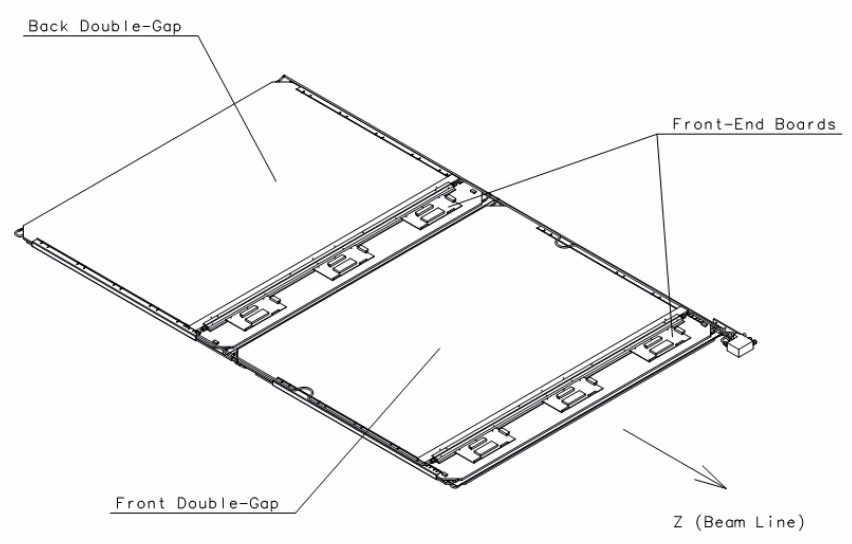
\includegraphics[width=0.45\textwidth]{figures/2rolls_chamber.png}}}\hfill
  \subfloat[][]{\label{subfig:3rolls}%
    \fbox{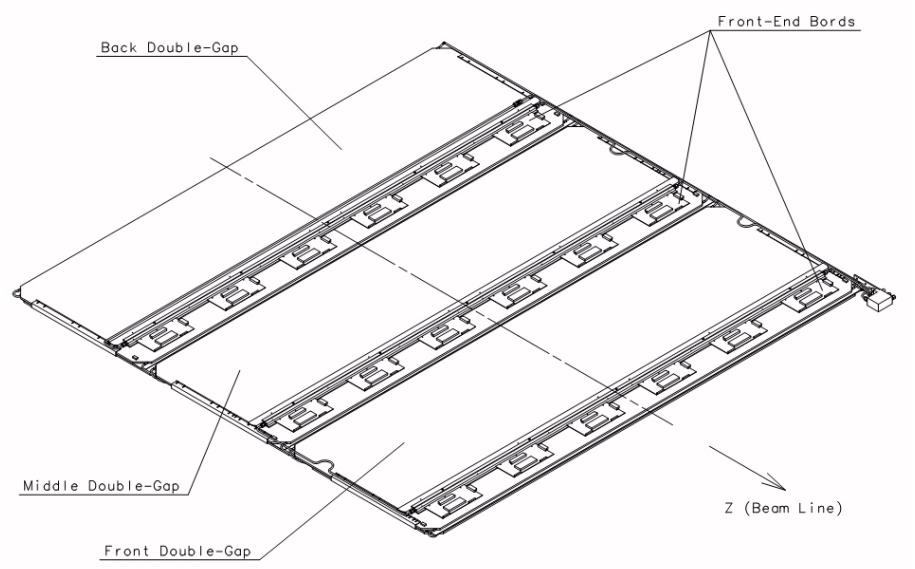
\includegraphics[width=0.46\textwidth]{figures/3rolls_chamber.png}}}\\
  \legend{Layout of chambers in CMS barrel divided into two rolls (a) and three rolls (b).}
  \source{\cite{CMS:2008xjf}}
\end{figure}

\section{CMS RPC Endcap}

In Endcap, there are 576 chambers divided into the 8 disks (RE$\pm$1, RE$\pm$2, RE$\pm$3, RE$\pm$4). Each disk have 72 chambers of trapezoidal shape divided in 2 concentric rings and 36 sectors. Each chamber is divided into 3 rolls, named A, B and C. The higher segmentation with respect to the barrel is driven by the higher particle multiplicity in the frontal regions. A layout of the Endcap geometry is shown in Fig. \ref{fig:RPC_endcap_layout}.

\begin{figure}[!htm]{15cm}
\caption{CMS RPC endcap layout}%
\label{fig:RPC_endcap_layout}
\fbox{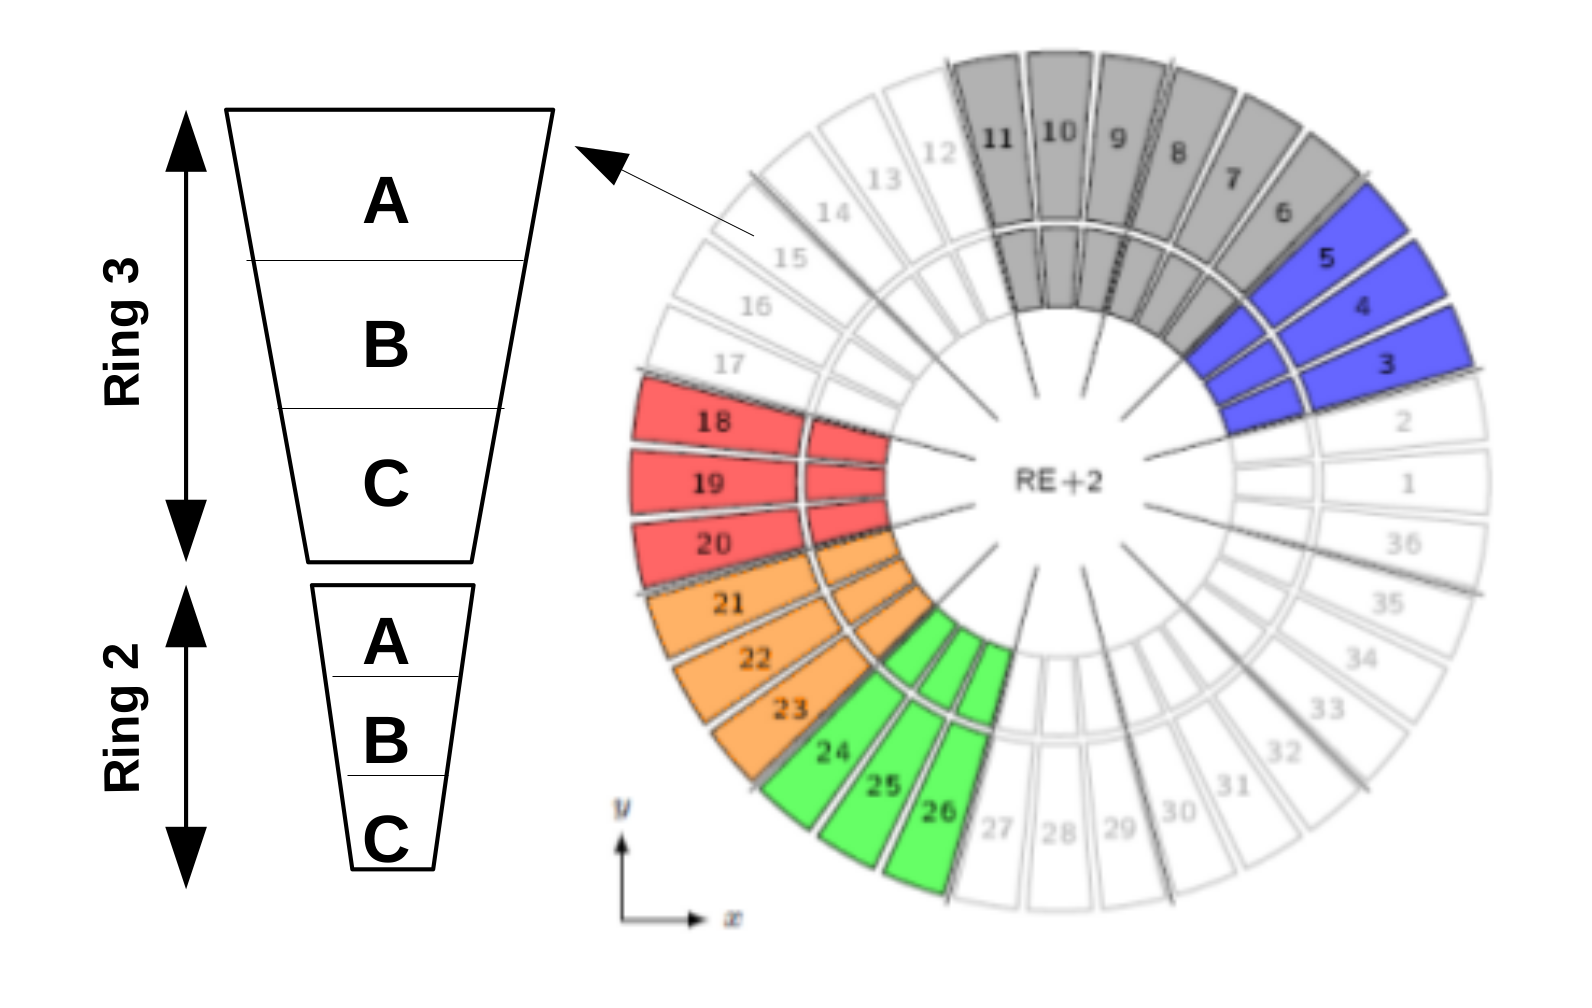
\includegraphics[width=.7\hsize]{figures/RPC_Endcap_layout.png}}
\legend{Layout of a RPCs placed in the CMS endcap region. They are distributed in 2 rings and 36 sectors for each disk.}
\source{\cite{CMSPublic:DPGRPC2016}}
\end{figure}

\section{RPC Upgrade for Phase-2}

The new requirements of the HL-LHC upgrade in terms of pile-up,  background and detector ageing will pose a big challenge for the correct muon identification and transverse momentum determination. The full muon system is preparing upgrades for the HL-LHC. In particular the RPC system is has two important foreseen developments.

The first upgrade is the replacement of the off-detector electronics (called link system). The current link system role is to process, synchronize and zero-suppress the signals coming from the RPC Front-End Boards (FEB) providing the RPC hits in a BX. The new link system will be able to deliver time of the hits, bringing the full timing potential of this detector. Also it will employ techniques and materials to suppress problems and deterioration caused by the high radiation environment.

And the second upgrade is the extension of the RPC coverage from |$\eta$| = 1.9 to 2.4 with the new improved RPC (iRPC) detectors. An extensive R\&D program is taking place to fulfil the demanding conditions of the HL-LHC. Two new RPC layers are going to be installed in the innermost rings of the disks RE$\pm$4 and RE$\pm$3. The new chambers will have a complete new design, with double-gap chambers with 1.4 mm thickness, to improve the time resolution. Also, the readout in two sides of the strip plane, allowing determination of the position in the 2D plane and a completely new front-end electronics. 

Regarding the current system, longevity tests are taking place at CERN GIF++ facility \cite{guida2015gif++}. The chambers are irradiated with a 12.6 TBq source in order to simulate the background conditions of the HL-LHC. The chambers showed stable performance with rates up to 600 Hz/cm$^2$ up to 93\% of the expected integrated charge \cite{Aly_2022}.

A complete review of the muon system upgrade can be found in \cite{CERN-LHCC-2017-012}.

\section{Author's contribution on the CMS RPC Project}

During the course of the PhD, there were many opportunities to contribute to the CMS RPC project. This section highlights the author most important contributions.

\subsection{Standard maintenance during Long Shutdown 2}

From December 2018 to March 2022, the LHC machine ceased operation for maintenance and upgrades in the accelerator complex in a period called Long Shutdown 2 (LS2). This time was an important moment for CMS maintenance and upgrades in preparation for the next data taking period (Run-3). In particular, the CMS RPC system underwent a intensive maintenance program to recover as much as possible the defects of the system system. In preparation for the future installation of the iRPCs chambers cooling and cable services for the new detectors were installed.

An extensive HV and low voltage (LV) maintenance campaign was performed. The goal of HV maintenance was to identify the problematic parts of the HV power system and to fix it in the best possible way, recuperating the performance of the chambers. A RPC chamber can have problems in one of the gaps or both, when the problem is in one of the gaps the efficiency pf such chamber can decrease as much as 15 \%, but it is recoverable with the increase of the applied HV, although it is not optimal as the current increases and the chamber's longevity is affected. 

The problems in HV were normally in one of the HV connectors, either because of bad connection, which was solved by a proper connection, or by defective connector, as shown in Fig. \ref{fig:HV_crack}. If this was the case, a the replacement of the connector or the use of spare channels was enough to bring back the gap to a good performance. In some cases the gaps itself were problematic, for example, because of problems with gas leakage. A total of 65 HV channels were repaired during LS2. 

\begin{figure}[!htm]{15cm}
\caption{Defective HV connector}%
\label{fig:HV_crack}
\fbox{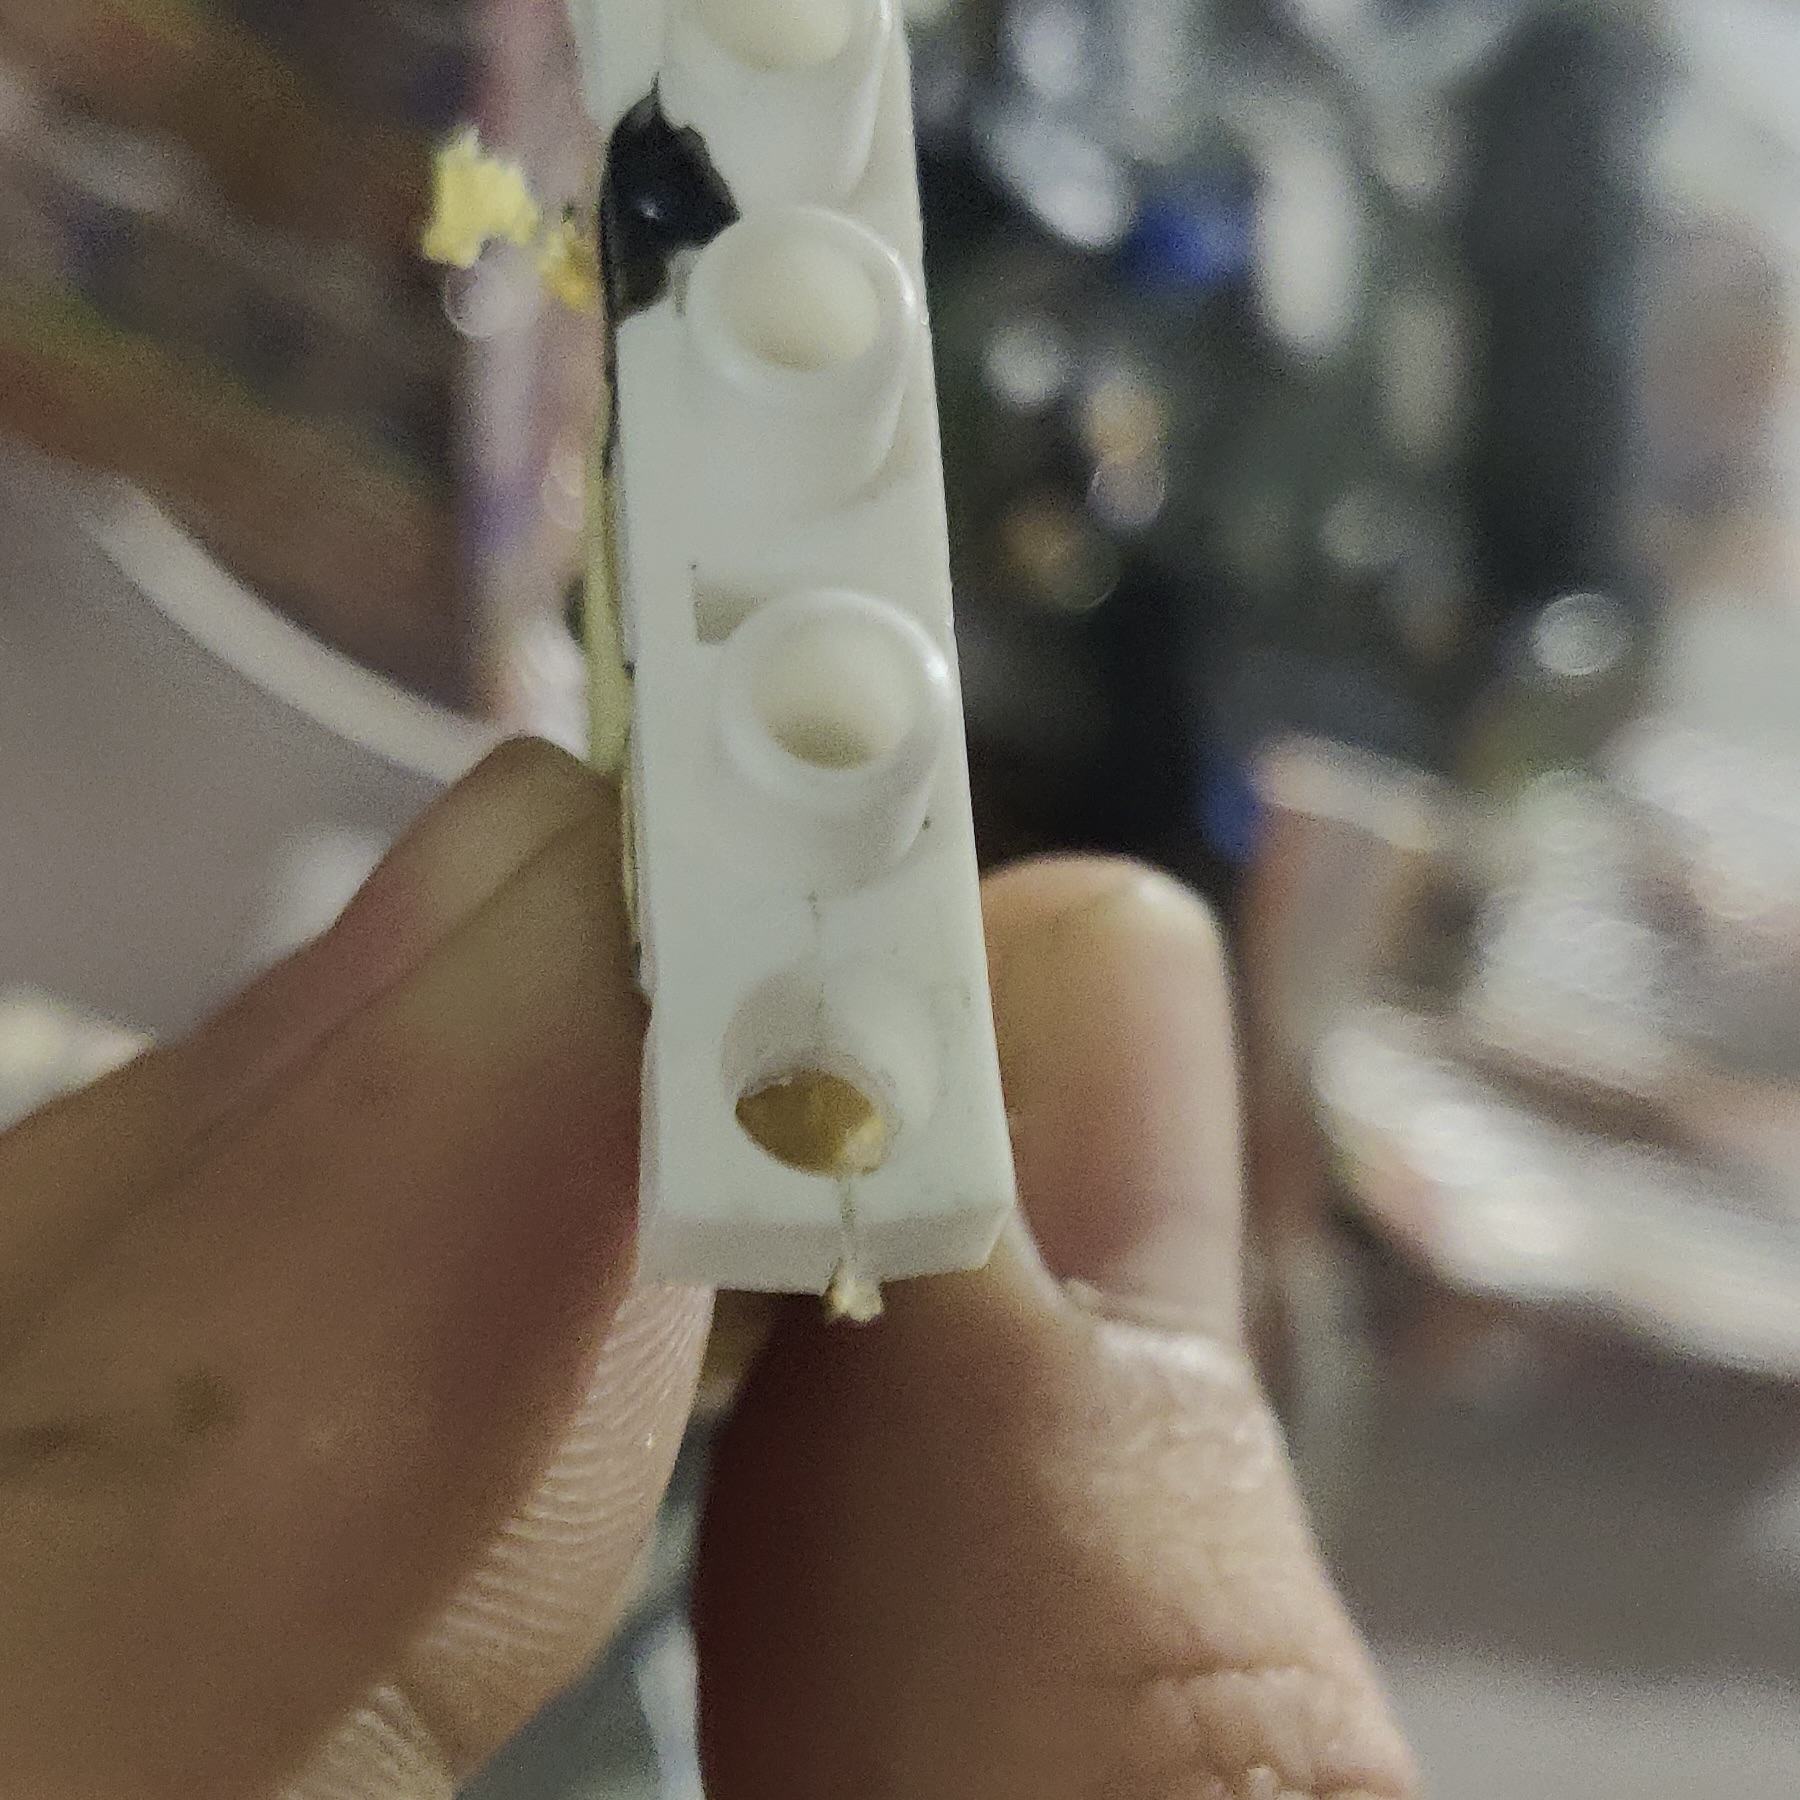
\includegraphics[width=.7\hsize]{figures/HV_crack.jpg}}
\legend{Example of defective HV connector. It is possible to see a crack in the connector on the bottom of the image. This problem compromises the proper isolation of the HV connector, leading to sparks.}
\end{figure}

The LV maintenance aim was to ensure a proper operation and configuration of the detector electronics and ensure a good functionality of the LV power boards and communication buses. A total of 12 LV problems were fixed.

Another important activity was the extraction of the chambers from the two RE4 stations to allow the CSC ME4/1 chambers extraction for electronics  refurbishment. The chambers were brought to the surface, and accommodated to a new laboratory with controlled environmental conditions and the infrastructure needed to test them (HV, LV and gas). All needed reparation and re-validation was done in this laboratory, before all the chambers were installed back.

The most priority activity, was gas system consolidation. The aim was to minimize the environmental impact of the RPC system. The actions taken were:
\begin{itemize}
    \item Gas Leak identification and repair. Often, the problems with the gas leaks were because of broken gas pipes and inlets inside the chambers. A endoscope was employed to find the problematic points and reparation was done when accessible. Figure \ref{fig:gas_problems} shows examples of problems found with the endoscope. Out of the identified 122 leaky chambers in barrel 49 where repaired, 14 are non-recoverable.
    \item Recuperation of the Exhaust, which was not working during Run-2 for the installation of the first C2H2F4 recuperation system with efficiency of 80 \%, which have been developed by CERN EP-DT Gas team \cite{Corbetta:2020esl}.
    \item Installation automatic pressure regulation valves on the redistribution gas racks to minimize pressure variations in the chambers, which can be a possible source of new leaks.
    \item Turn off the remaining leaky chambers which was not possible to repair, to keep the amount of fresh gas added to the system at a minimum.
\end{itemize}
A summary of the activities in LS2 can be found in \cite{Amarilo_2022}.

\begin{figure}[!htm]{15cm}
  \caption{Gas problems inside RPC chambers.} 
  \label{fig:gas_problems}
  \subfloat[][]{\label{subfig:gas_crack}%
    \fbox{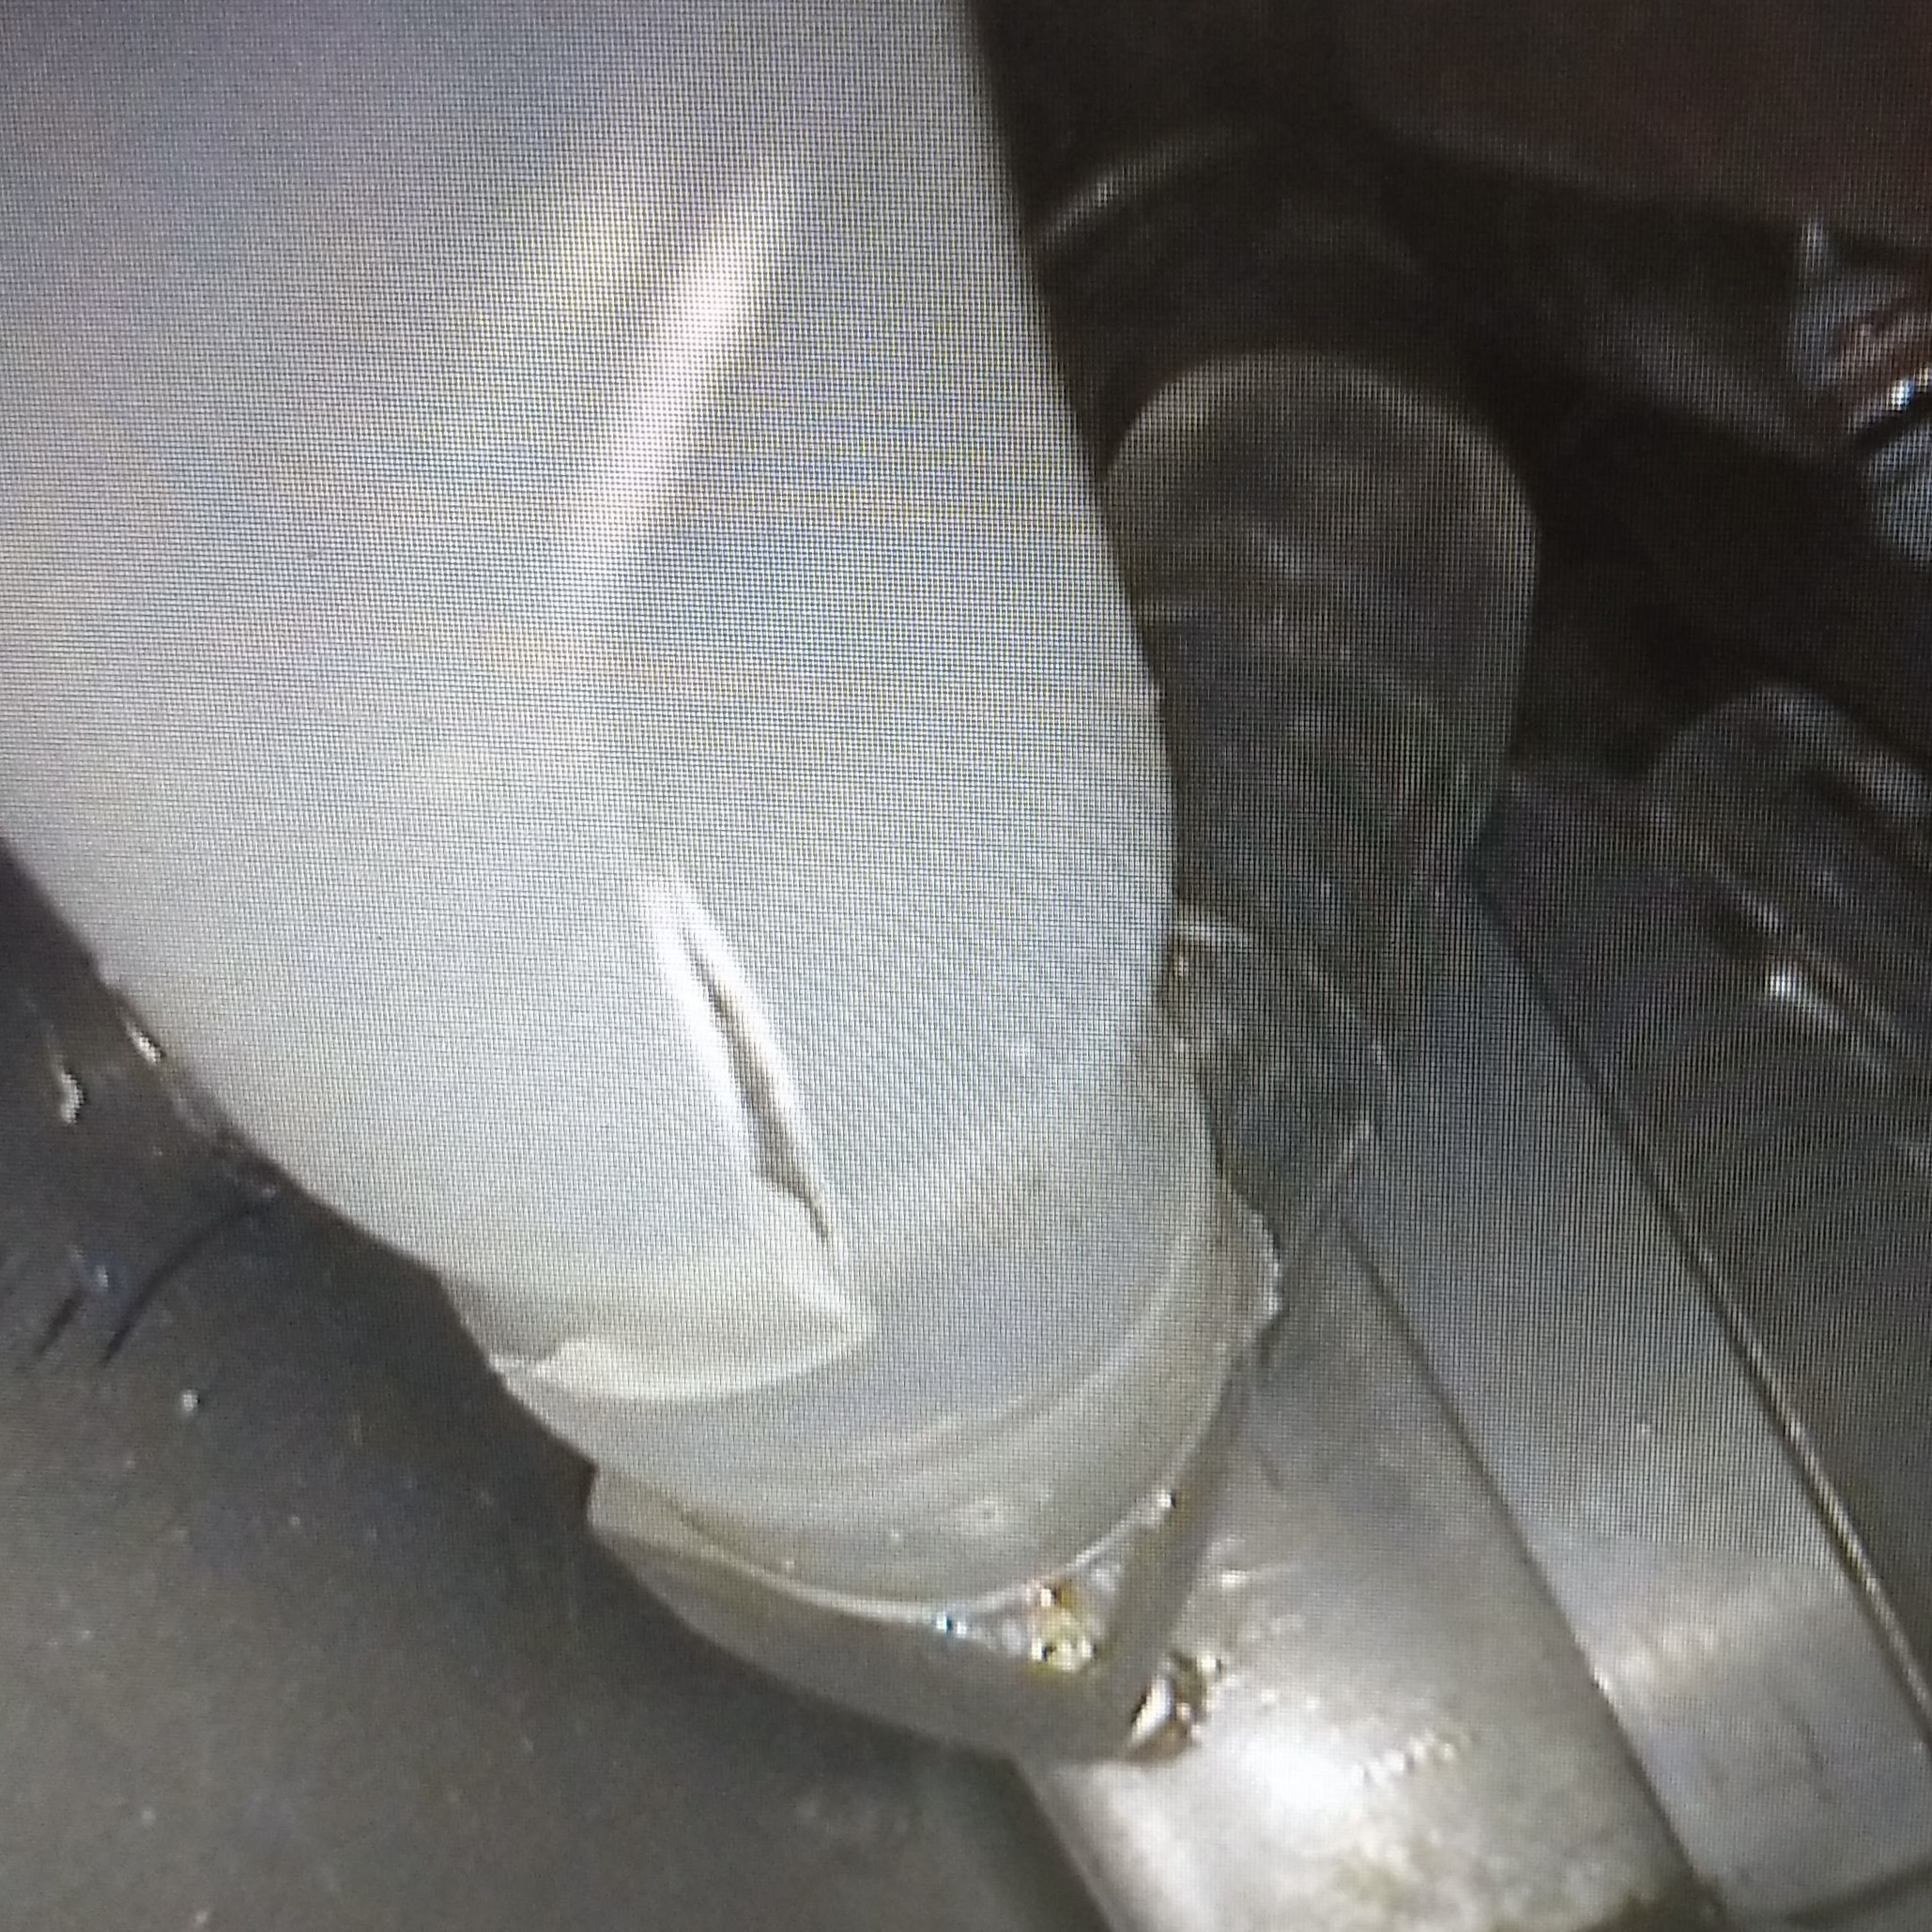
\includegraphics[width=0.45\textwidth]{figures/gas_crack.jpg}}}\hfill
  \subfloat[][]{\label{subfig:gas_break}%
    \fbox{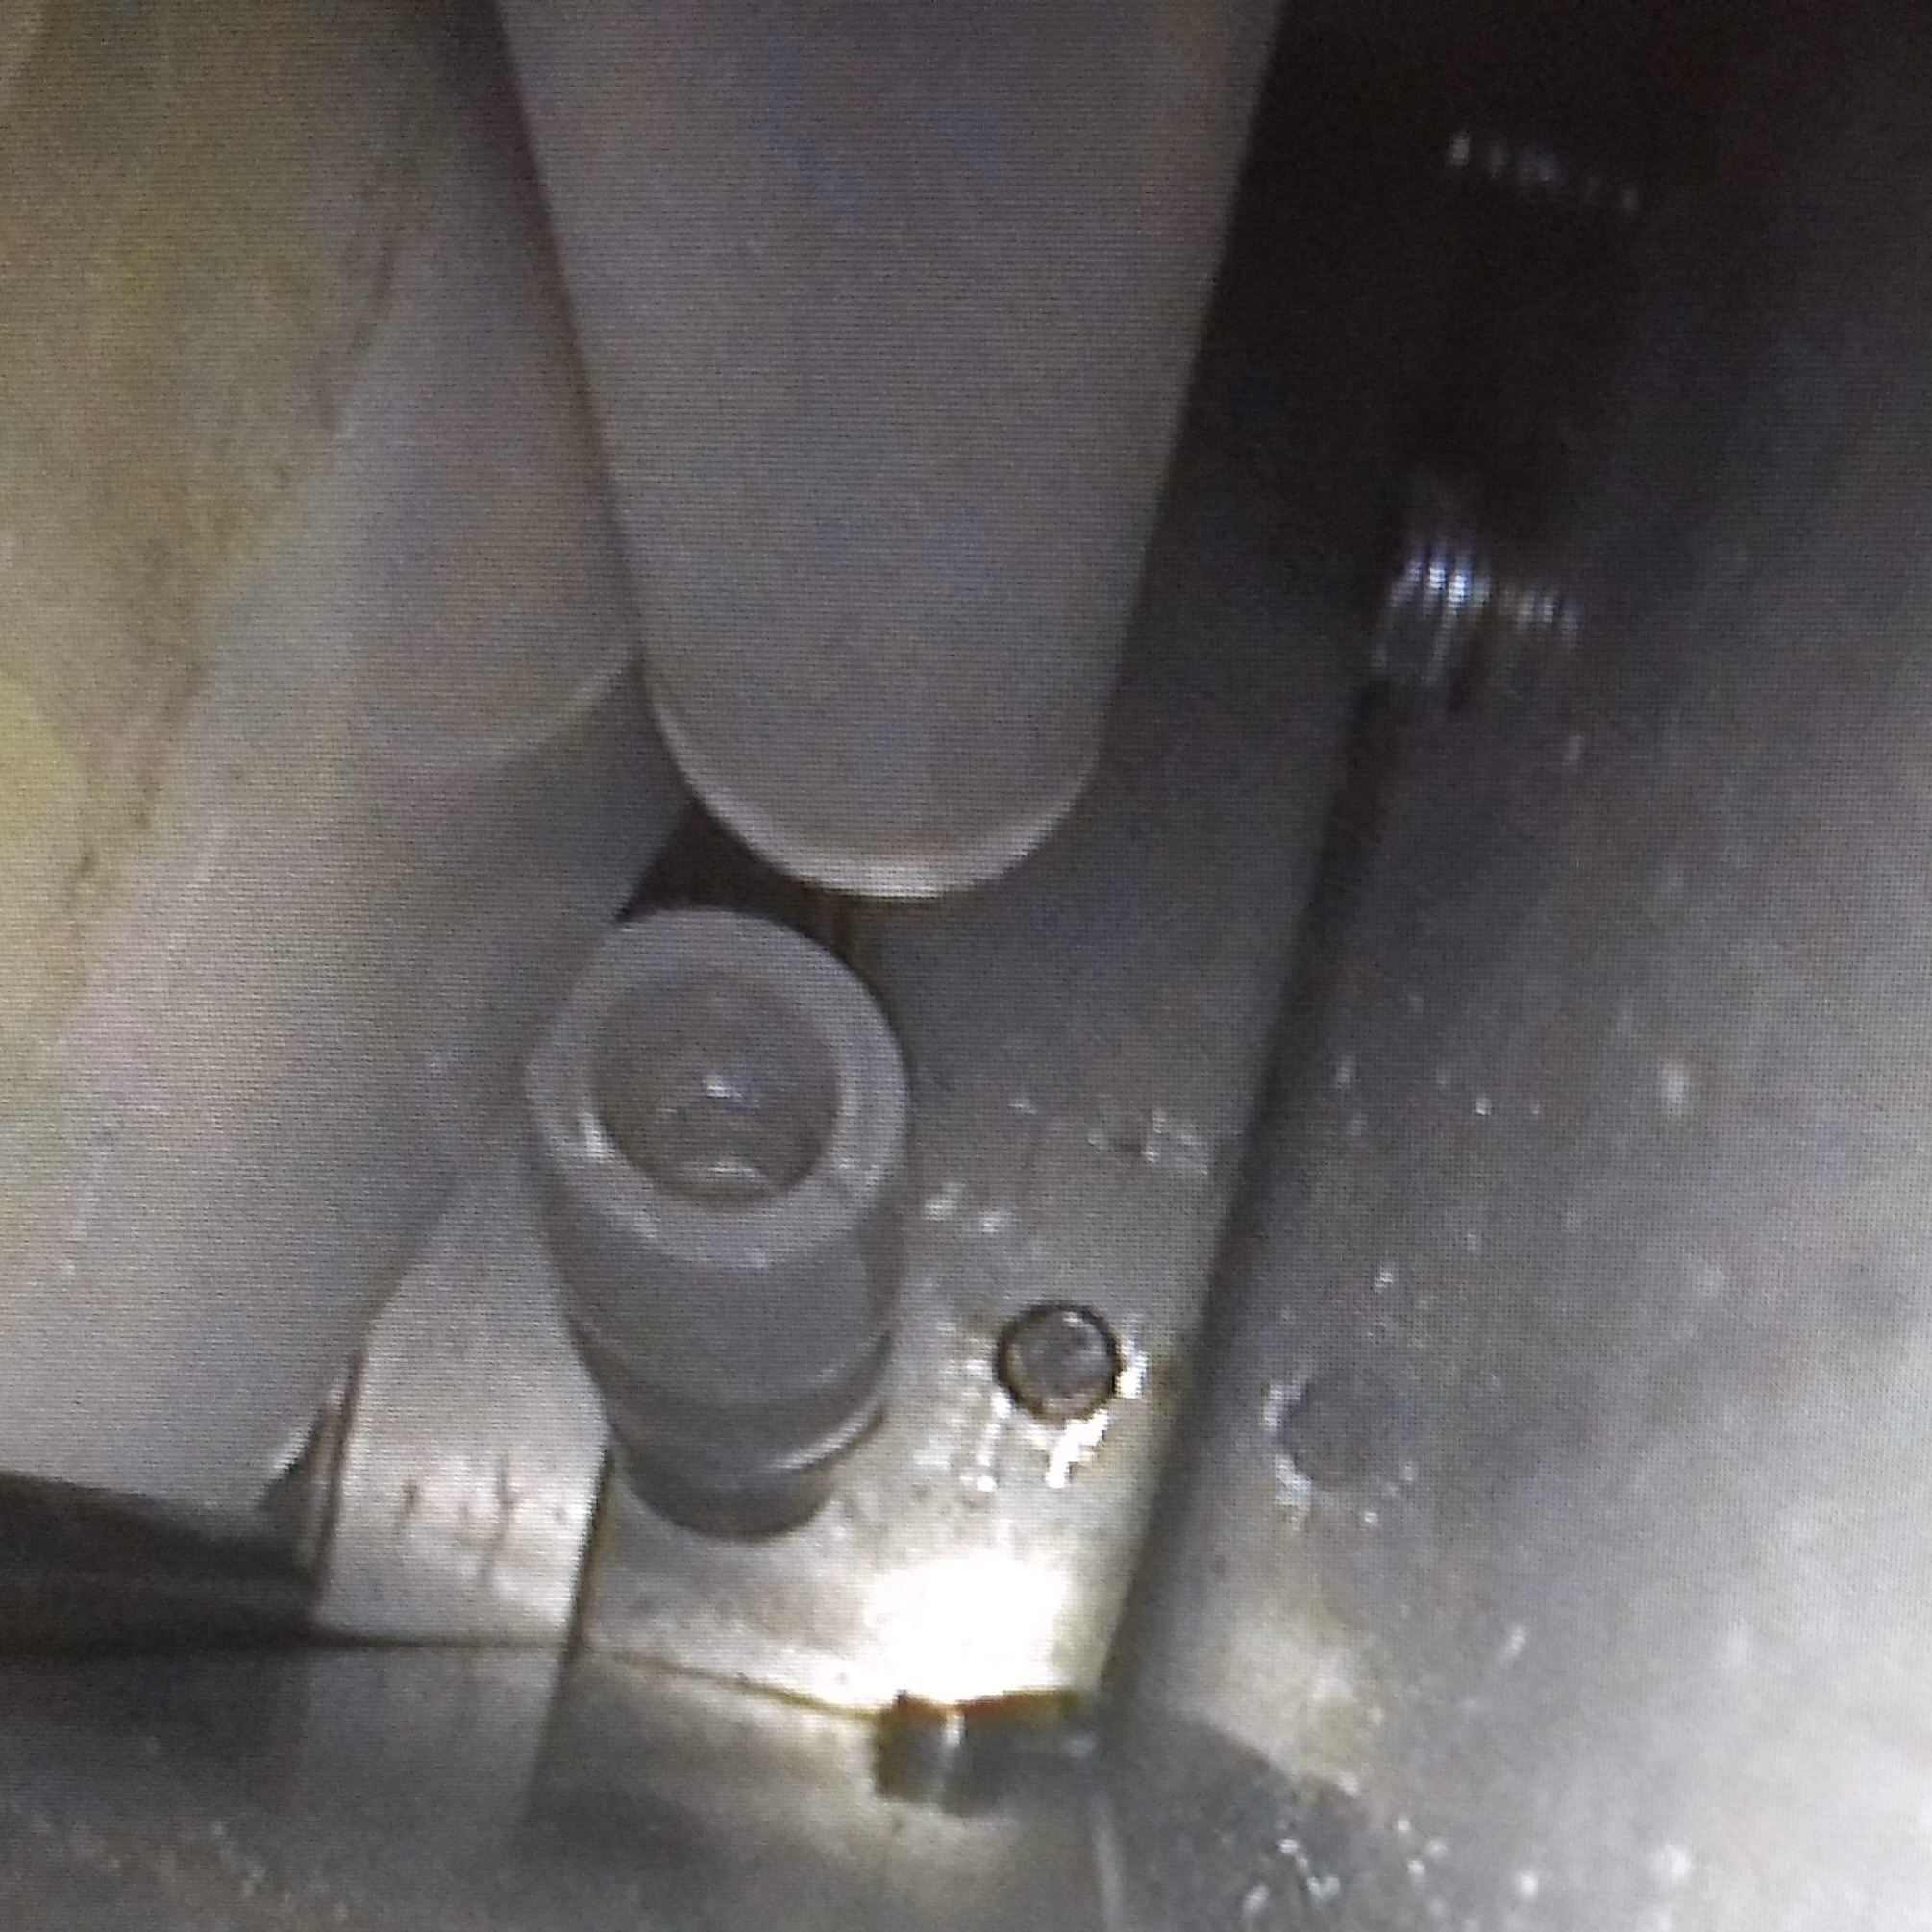
\includegraphics[width=0.45\textwidth]{figures/gas_broken.jpg}}}\\
  \legend{Pictures taken during endoscopic inspection to find gas problems inside RPC chambers. a crack in the pipe is found in (a) and a completely cut pipe in (b)}
\end{figure}

The performance of the repaired chambers can be seen in Figs. \ref{fig:repaired_gas} and \ref{fig:repaired_HV} as a comparison between cosmic-rays data-taking of 2018 and 2021. There was great improvement, 34 rolls were recovered by gas leak repairs and the HV repairs translated into a gain of ~6\% in the efficiency of these chambers. Overall, the results of the repairs were successful bringing higher efficiency to the repaired channels. In Fig. \ref{fig:overallefficiency2018vs2022} a comparison of the distribution of roll efficiency in pp collisions taken in 2018 and 2022 is given for barrel and endcap and the results mentioned are confirmed.

\begin{figure}[!htm]{15cm}
\caption{Performance of repaired gas leak chambers in cosmic data taking}%
\label{fig:repaired_gas}
\fbox{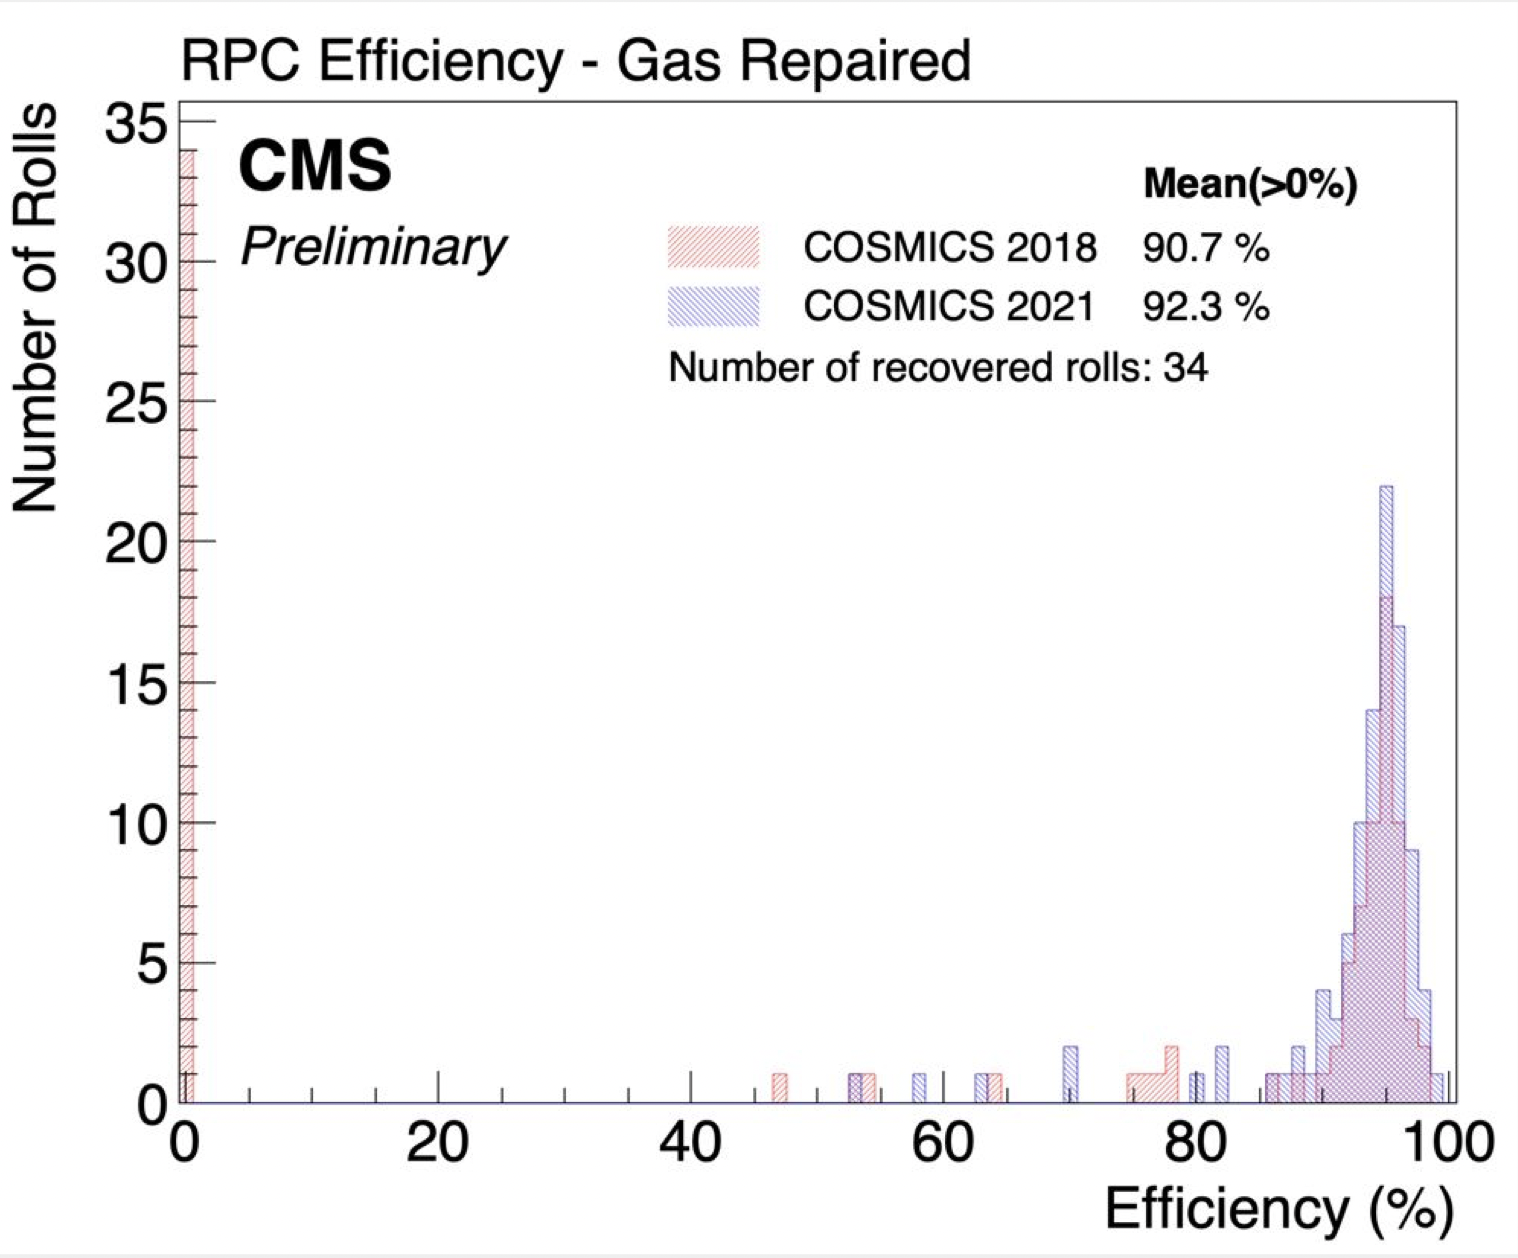
\includegraphics[width=.5\hsize]{figures/Repaired_gas.png}}
\legend{The distribution of efficiency of RPC rolls on gas repaired chambers during the Long Shutdown 2 (LS2). Using cosmics data taking in 2018 (red) and 2021 (blue) for barrel region. The numbers show a significant improvement, with respect to 2018 as 34 OFF rolls from Run-2 are recovered and HV is repaired for several chambers recovering chambers from Single Gap to Double Gap operation mode.}
\source{\cite{CMSPublic:DPGRPC2021}}
\end{figure}

\begin{figure}[!htm]{15cm}
\caption{Performance of repaired gas leak chambers in cosmic data taking}%
\label{fig:repaired_HV}
\fbox{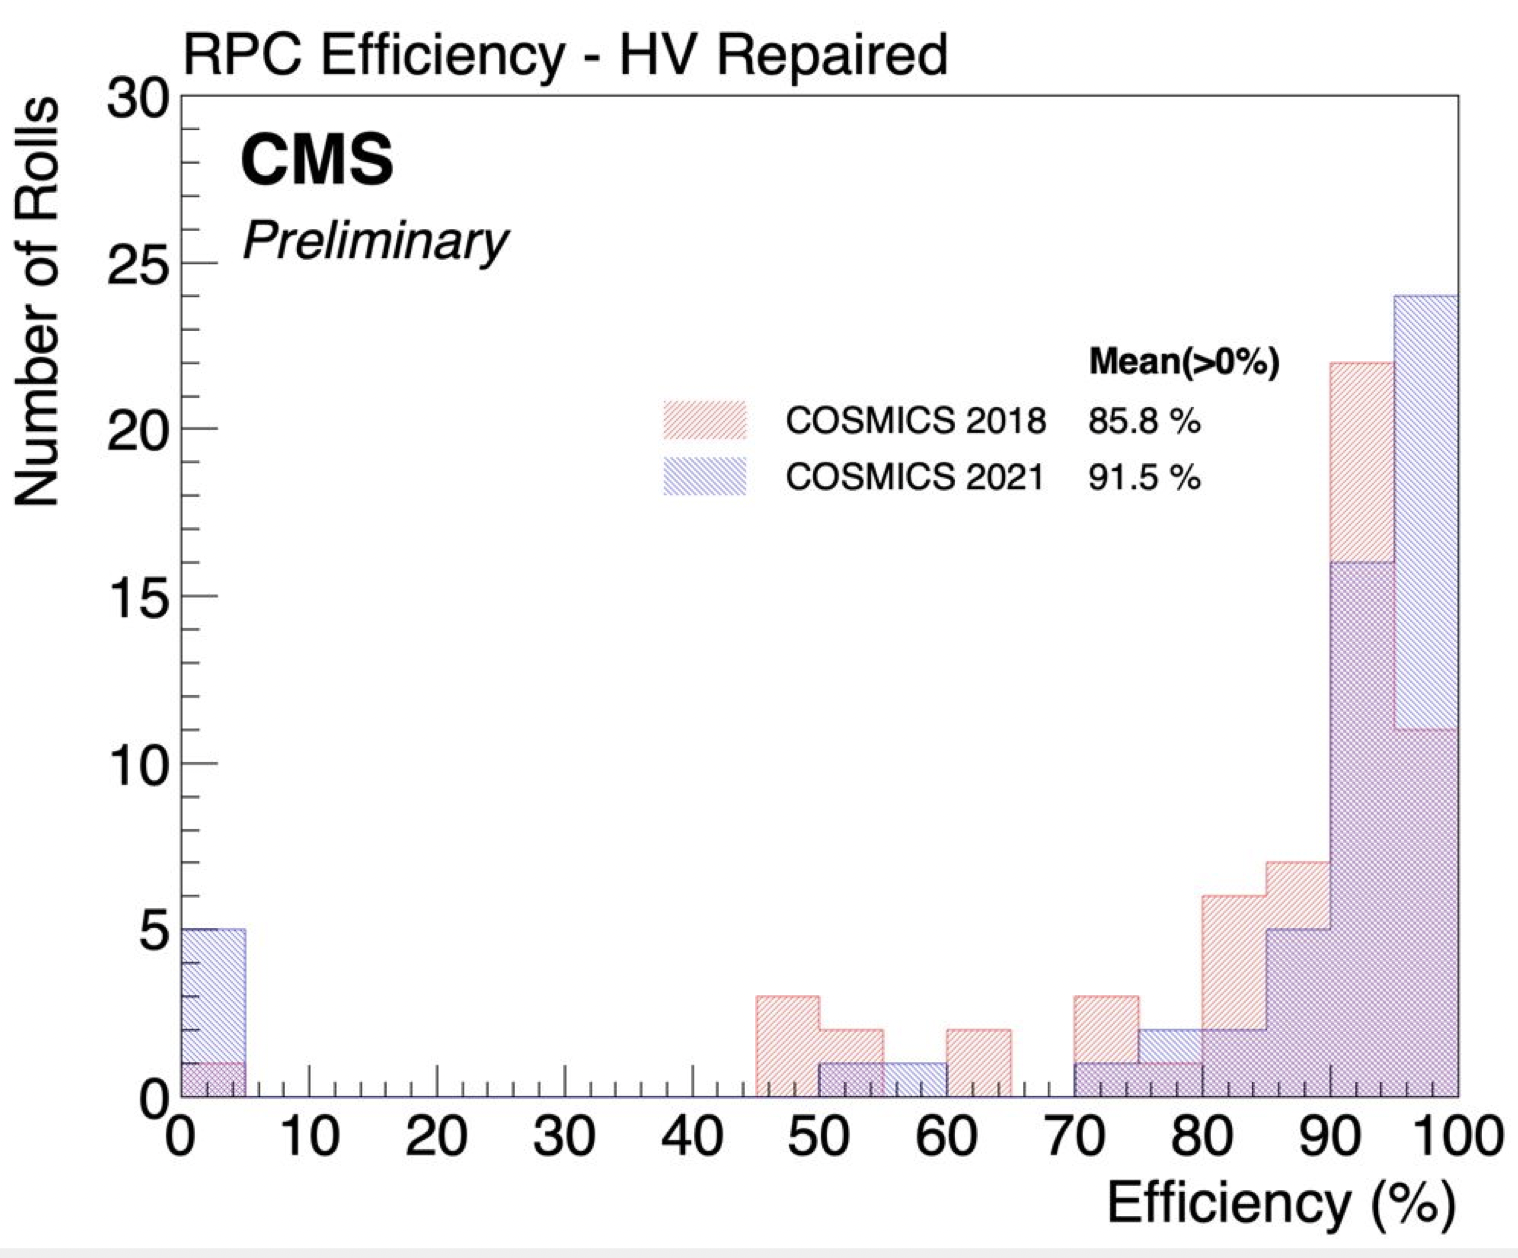
\includegraphics[width=.5\hsize]{figures/Repaired_HV.png}}
\legend{The distribution of efficiency of RPC rolls on HV repaired chambers during the Long Shutdown-2 (LS2) using cosmics data taking in 2018 (red) and 2021 (blue) for barrel region. The RPC efficiencies measured in 2021, after LS2 are comparable and in agreement with the expectations. The overall efficiency is improved by ~6\% due to recovery of chambers from Single Gap to Double Gap operation mode.}
\source{\cite{CMSPublic:DPGRPC2021}}
\end{figure}

\begin{figure}[!htm]{15cm}
  \caption{Overall RPC efficiency in pp collisions.} 
  \label{fig:overallefficiency2018vs2022}
  \subfloat[][]{\label{subfig:overallefficiency2018vs2022barrel}%
    \fbox{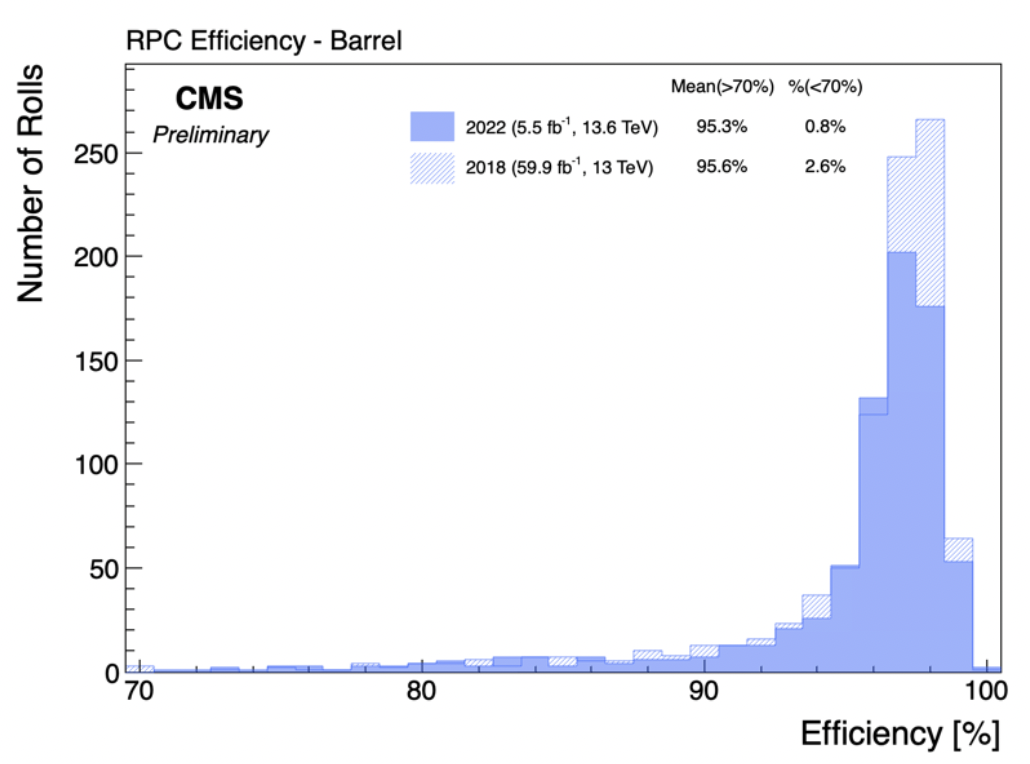
\includegraphics[width=0.45\textwidth]{figures/Efficiency_Barrel.png}}}\hfill
  \subfloat[][]{\label{subfig:overallefficiency2018vs2022endcap}%
    \fbox{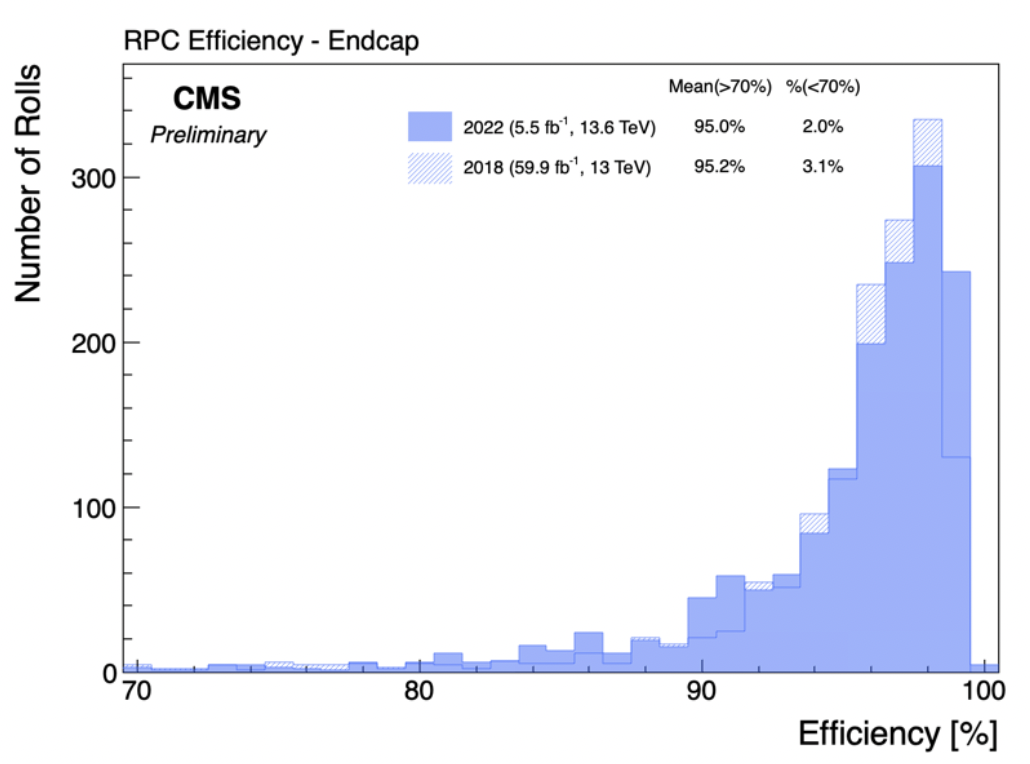
\includegraphics[width=0.45\textwidth]{figures/Efficiency_Endcap.png}}}\\
  \legend{Comparison of the overall RPC efficiency in 2018 and 2022 in pp collisions data taking. The barrel chambers are plotted in (a) and the endcap ones in (b).}
  \source{\cite{CMSPublic:DPGRPC2022}}
\end{figure}

\subsection{RPC Detector Control System}

A big experiment like CMS need a control software for all the required needs for control, monitoring and safe operation of its subsystems. The WinCC\footnote{formerly known as PVSS} SCADA (Supervisory Control And Data Acquisition) software together with the Joint Control Project (JCOP) framework form the basis of the Detector Control System (DCS) for the big experiments at LHC \cite{Arcidiacono:2005fr}. 

Each subsystem at CMS is tasked to develop the DCS for itself to be able to react to the commands passed from the CMS Central DCS. The RPC DCS is divided into several subsystems that are part of the infrastructure needed for the operation of the RPCs chambers as shown in Figure \ref{fig:RPC_DCS_layout}. Each subsystem communicates with DCS, passing information that is archived in a ORACLE database and receiving commands.

\begin{figure}[!htm]{15cm}
\caption{CMS RPC DCS layout}%
\label{fig:RPC_DCS_layout}
\fbox{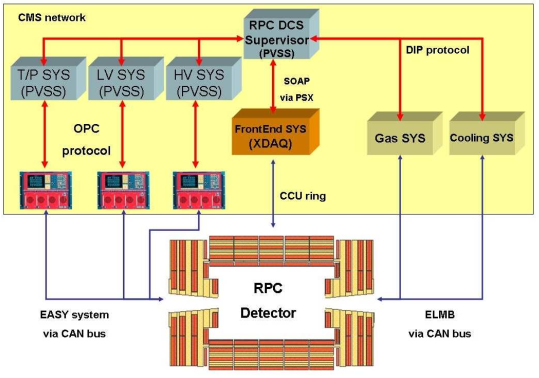
\includegraphics[width=\hsize]{figures/RPC_DCS_subsystems.png}}
\legend{The CMS RPC DCS layout, displaying all its subsystems.}
\source{\cite{Polese:2010zz}}
\end{figure}

The Power system for HV and LV is based on the CAEN EASY project \cite{CAENEASY}. It is designed to operate in hostile areas (high radiation and magnetic field strength) and connected to the DCS through the OPC protocol \cite{OPCFoundation}.  Temperature and relative humidity (RH) sensors are read by ADCs connected to the CAEN EASY system and sent to DCS. The gas infrastructure data is acquired from Programmable Logic Controllers and distributed via DIP \cite{Barillere:2003fi}. In the same way all the information concerning the CMS infrastructure, (e.g. Cooling, Detector Safety System (DSS), LHC and Magnet status), is available through DIP. Finally, FEB information is available through XDAQ, the online CMS framework, using SOAP (Simple Object Access Protocol)  messages to PSX \cite{gutleber2002software}.

All this control subsystems are able to run by itself as components of the RPC system. However, all the information is gathered around a hierarchical hierarchical double-tree control structure, shown in Fig. \ref{fig:RPC_DCS_structure}, implemented through a Finite State Machine (FSM). This automation schema reduces the amount of human intervention in the system, for all the repetitive tasks, and optimize recovery procedures in case of undesired states. The FSM is defined by its states and the commands. The states are:
\begin{itemize}
    \item ON - RPC is ready for data taking.
    \item STANDBY - High voltages are on standby voltage (6500 V for the CMS RPCs and 5000 V for the iRPCs), low voltages are on. It is used as a safe state.
    \item OFF - Both high voltages low voltages are switched-off.
    \item RAMPING - A transitional state, while the High voltage is moving to the desired set point.
    \item ERROR - A manual intervention is required and no data taking is possible.
\end{itemize}
The commands are ON, OFF and STANDBY, which effectuates the transitions to the states with same name.

\begin{figure}[!htm]{15cm}
\caption{CMS RPC hierarchy tree}%
\label{fig:RPC_DCS_structure}
\fbox{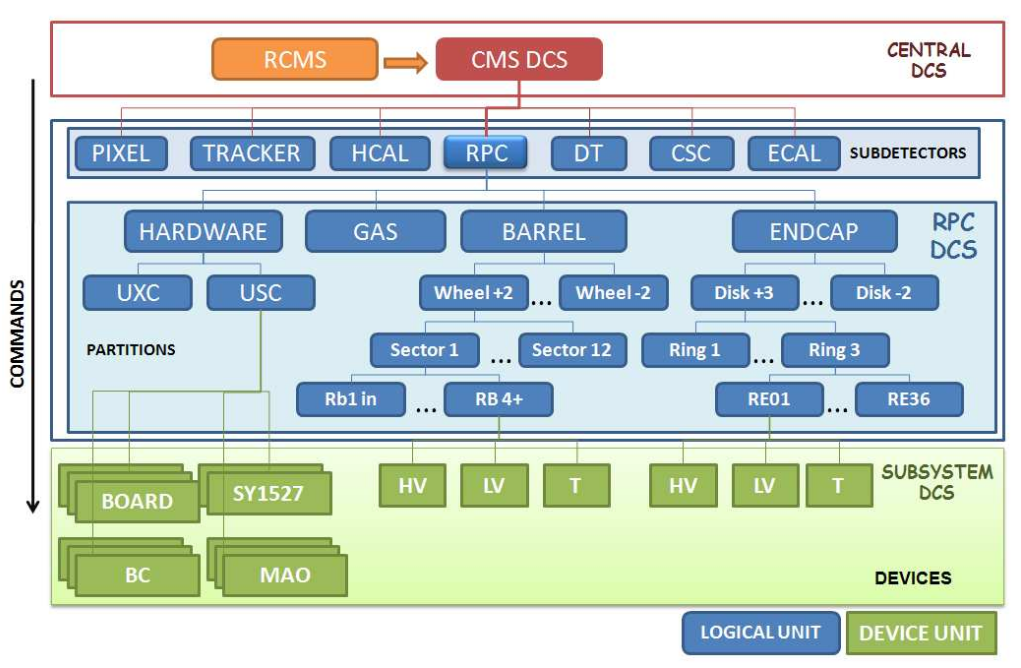
\includegraphics[width=\hsize]{figures/RPC_DCS_Structure.png}}
\legend{Structure of the hierarchy tree of the RPC DCS. Different branches describe the
RPC system from the geographical and hardware points of view. All commands go down the
hierarchy, while information and error messages are reported upwards.}
\source{\cite{Polese:2010zz}}
\end{figure}

The WinCC software can also be used to develop a Graphical User Interface (GUI). It is developed to be a easy way for the user interact to the system, being able to control and monitor the desired parameters of the system, as well as display the important alerts. It is structured in approximately 40 panels to provide easy visualization and navigation through the system structure. The GUI can be accessed remotely, which is very important for a collaboration with people from different countries in the world, like CMS, and provides a authentication system, to prevent use from non-experts. Figure \ref{fig:RPC_DCS_GUI} displays a overview of the RPC DCS GUI.

\begin{figure}[!htm]{15cm}
\caption{CMS RPC DCS GUI overview}%
\label{fig:RPC_DCS_GUI}
\fbox{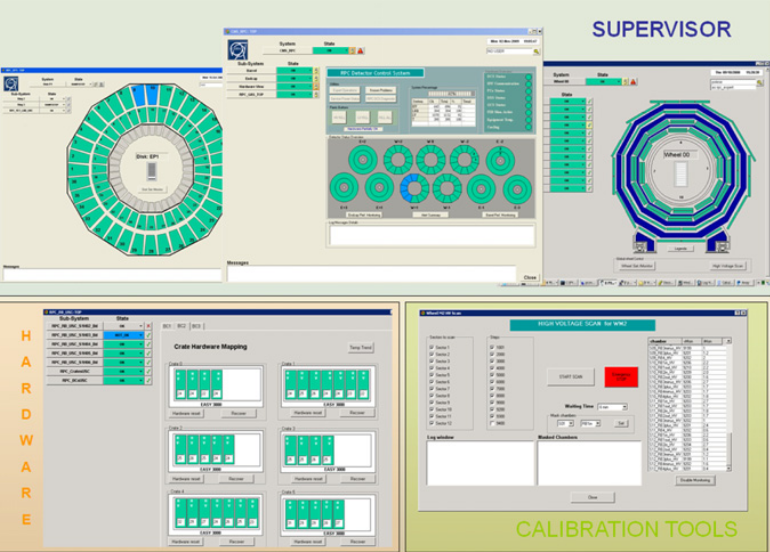
\includegraphics[width=\hsize]{figures/RPC_DCS_GUI.png}}
\legend{Overview of the CMS RPC DCS GUI. The panels are formed with a combination of widgets and texts to better display the system structure.}
\source{\cite{Polese:2012zz}}
\end{figure}

More details on the design of the RPC DCS can be found in \cite{Polese:2010zz, Polese:2012zz}

The work done at the CMS RPC DCS were the update of the system for the upgrade from WinCC version 3.15 to 3.16, which introduced some breaking changes, so the current software needed to be adapted to this new version. The correction of bugs and addition of new functionalities. The most important tasks were the creation of a new panel, shown in Fig. \ref{fig:RPC_DCS_Demo_panel}, for four iRPCs installed as a Demonstrator.

\begin{figure}[!htm]{15cm}
\caption{CMS RPC DCS Demonstrator panel}%
\label{fig:RPC_DCS_Demo_panel}
\fbox{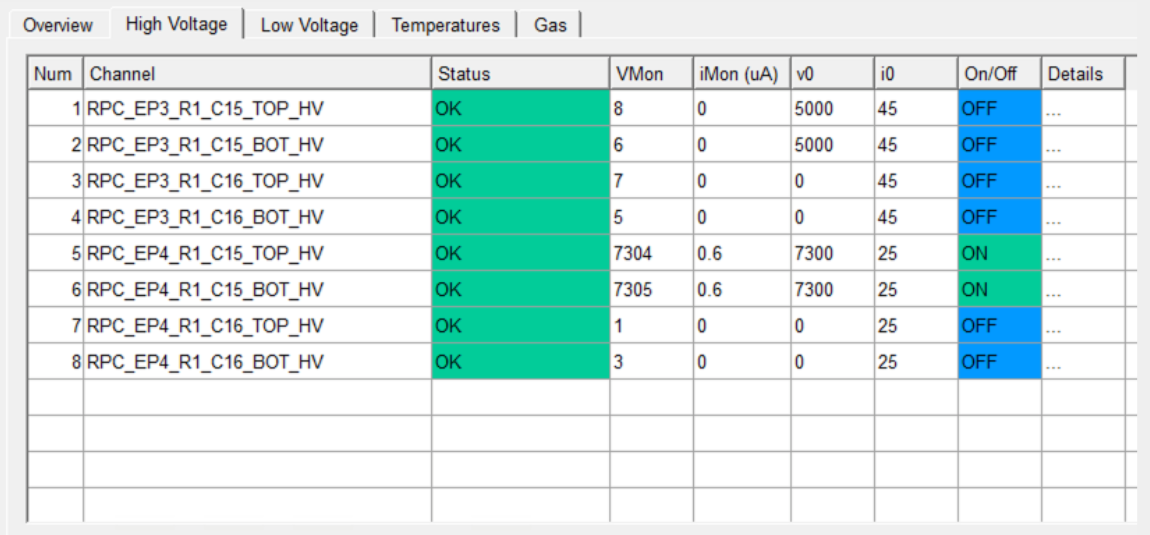
\includegraphics[width=\hsize]{figures/Demo_panel.png}}
\legend{New Panel at CMS RPC DCS for the iRPC demonstrator chambers control and monitoring}
\end{figure}

The most important task was the creation of a new database schema for the gas system. Because of the big changes in the gas system, due to the gas leaks, many channels had to be swapped and some of them switched off. This created the need to change the previous schema, which was chamber-based, to a new one, with abstractions for the gas racks, gas channels and the chambers. Furthermore, the gas flow cells used were found to not be precise enough in the gas flow measurements, that are very important to the determination of whether or not the chambers are leaking. This demanded the creation of three new tables in the database schema and update of the WinCC with the new abstraction. The tables were created also to facilitate the relationship between chambers, the geographical position and infrastructure they use (e.g. HV/LV/gas channels) and current ``health'' situation (any of the gaps are disconnected).

The gas flow for each one of the gas channels were calibrated by a linear function, which parameters were determined for each one of the flow cells by using a very precise mass flow meter. The DCS is also tasked to use these parameters to calculate the corrected flow.

\subsection{RPC-based tracking system at GIF++}

Another task developed for the RPC Project was to help in the test beams at CERN Gamma Irradiation Facility (GIF++), to measure the performance and longevity of the RPC and iRPC chambers in the HL-LHC conditions. 

GIF++ is a very singular facility, where a high energy particle beam (normally muons) and and photons from a gamma source (13 TBq, $^{137}$Cs), with adjustable flux, are combined \cite{guida2015gif++}. Tests for the muon detectors of several experiments (e.g. ATLAS, ALICE, CMS and SHiP) are taking place there.

The chambers must be validated up to the expected background rate: 600 Hz/cm$^2$ for the RPCs in the current CMS Muon system and up to 2 kHz/cm$^2$ for the new iRPCs (including the safety factor of three) \cite{CERN-LHCC-2017-012}. Such high rates can pose a challenge to the measurement, as the fake hits can bias the data-taking. So a tracking system made of RPCs was proposed to remove the background that comes from photons, taking into account the high efficiency of these chambers to muon and the fact that the photon can only be detected by the RPC after being converted to electrons, and the detection efficiency is low (< 1\%) \cite{Weizheng:2014ifa}.

The data acquisition is performed using a CAEN Time-to-Digital Converter (TDC) module of type V1190A where the front-end electronics of the chambers are connected. A V1718 VME controller module is responsible for the communication between the TDC and the computer where the data are stored. To host the VME controller and the TDC a 6U VME 6021 crate is used.

To determine the data taking with respect to the HV, several runs are taken for different HV points. The hits are recorded by the TDC with respect to a trigger based by a coincidence of scintillation detectors, as shown in Figure \ref{fig:RPC_hits_TDC}, all the hits are recorded in a time window of 5 $\mu$s. The triggered muons show a narrow peak in Fig. \ref{subfig:RPC_hits_TDC_muonspill}, so a time window is defined for the hits that are going to be taken into account for the efficiency calculation, in order to suppress the the majority of background from gammas. The time window is defined by doing a Gaussian fit to the time profile in the region of the peak and a window of 6 times sigma, centred in the mean of the fitted Gaussian is taken as the muon window, as given by Fig. \ref{subfig:RPC_hits_TDC_zoomed}.

\begin{figure}[!htm]{15cm}
  \caption{RPC hits recorded by a TDC at GIF++.} 
  \label{fig:RPC_hits_TDC}
  \subfloat[][]{\label{subfig:RPC_hits_TDC_muonspill}%
    \fbox{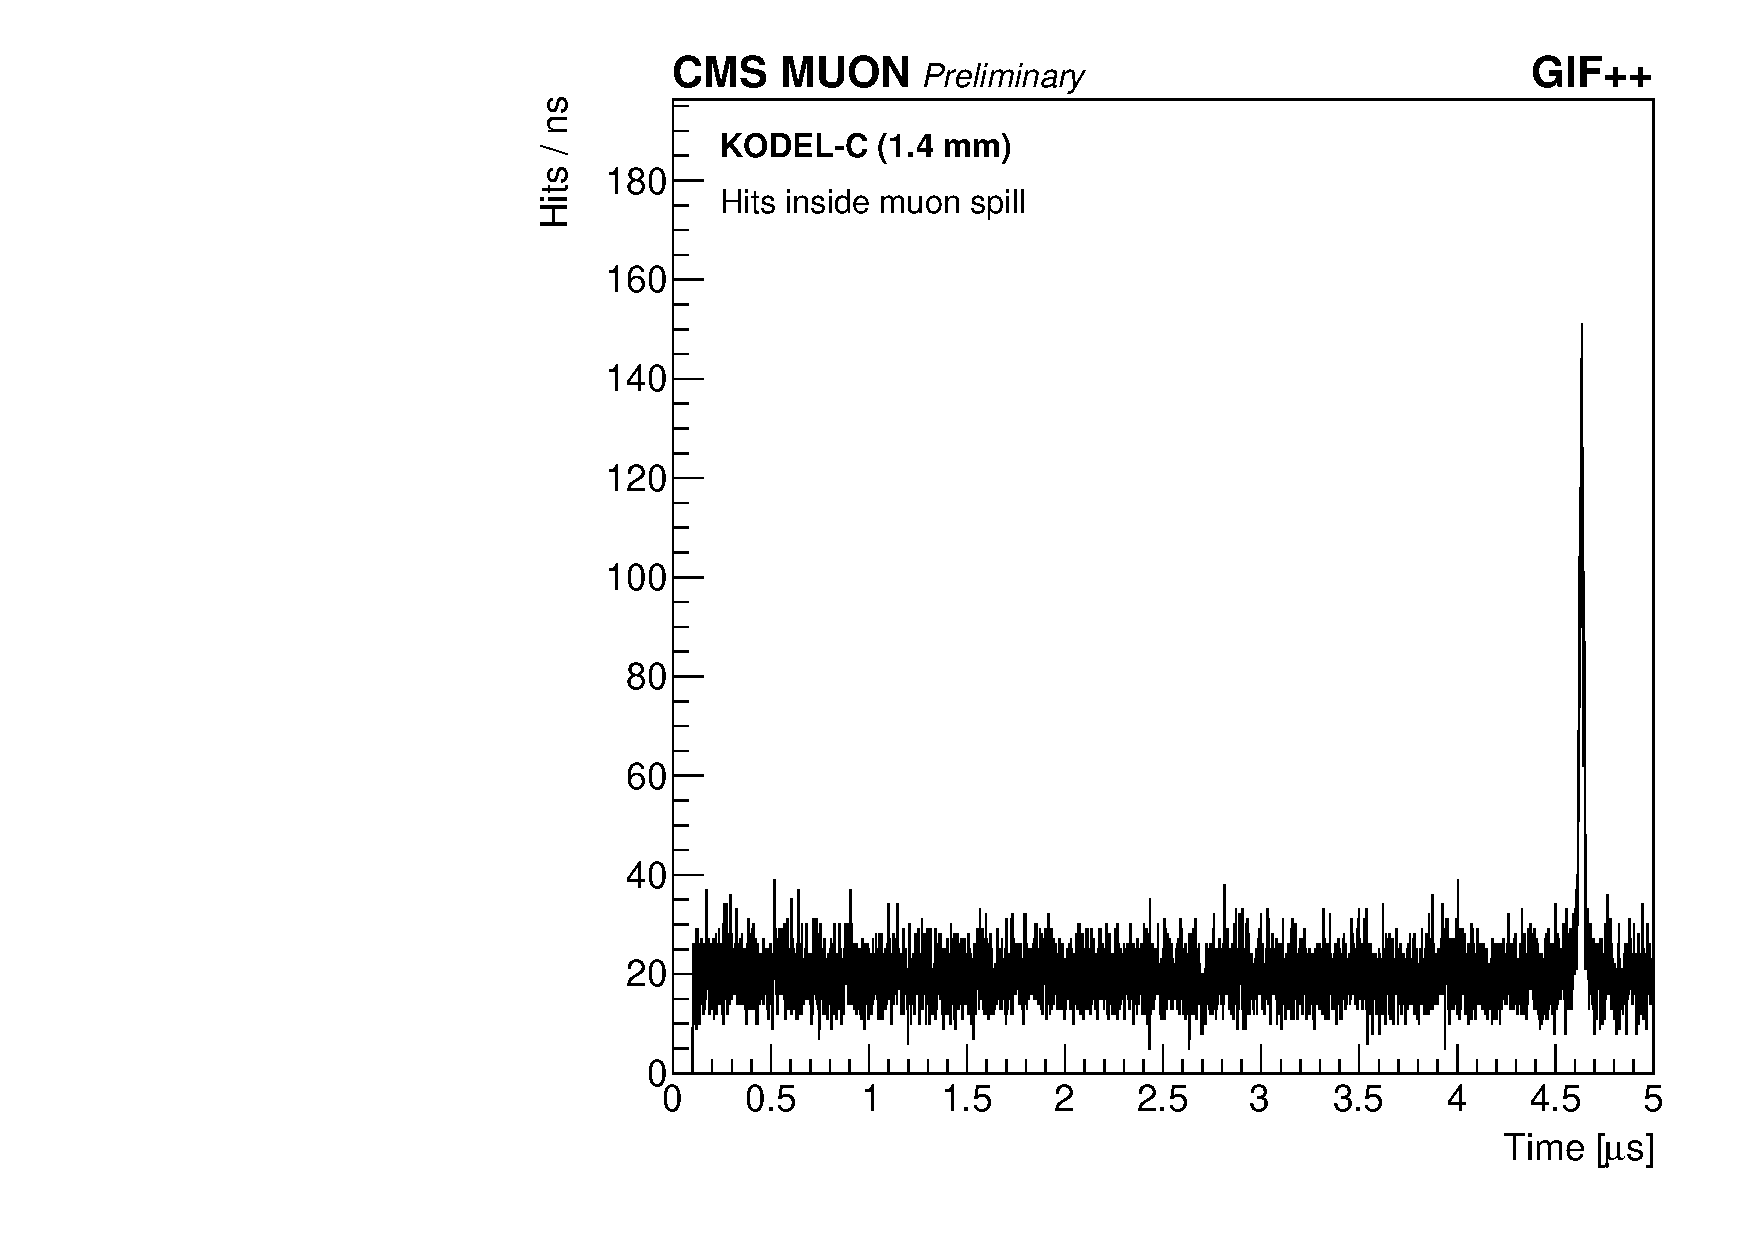
\includegraphics[width=0.45\textwidth]{figures/timeProfile_spill.pdf}}}\hfill
  \subfloat[][]{\label{subfig:RPC_hits_TDC_zoomed}%
    \fbox{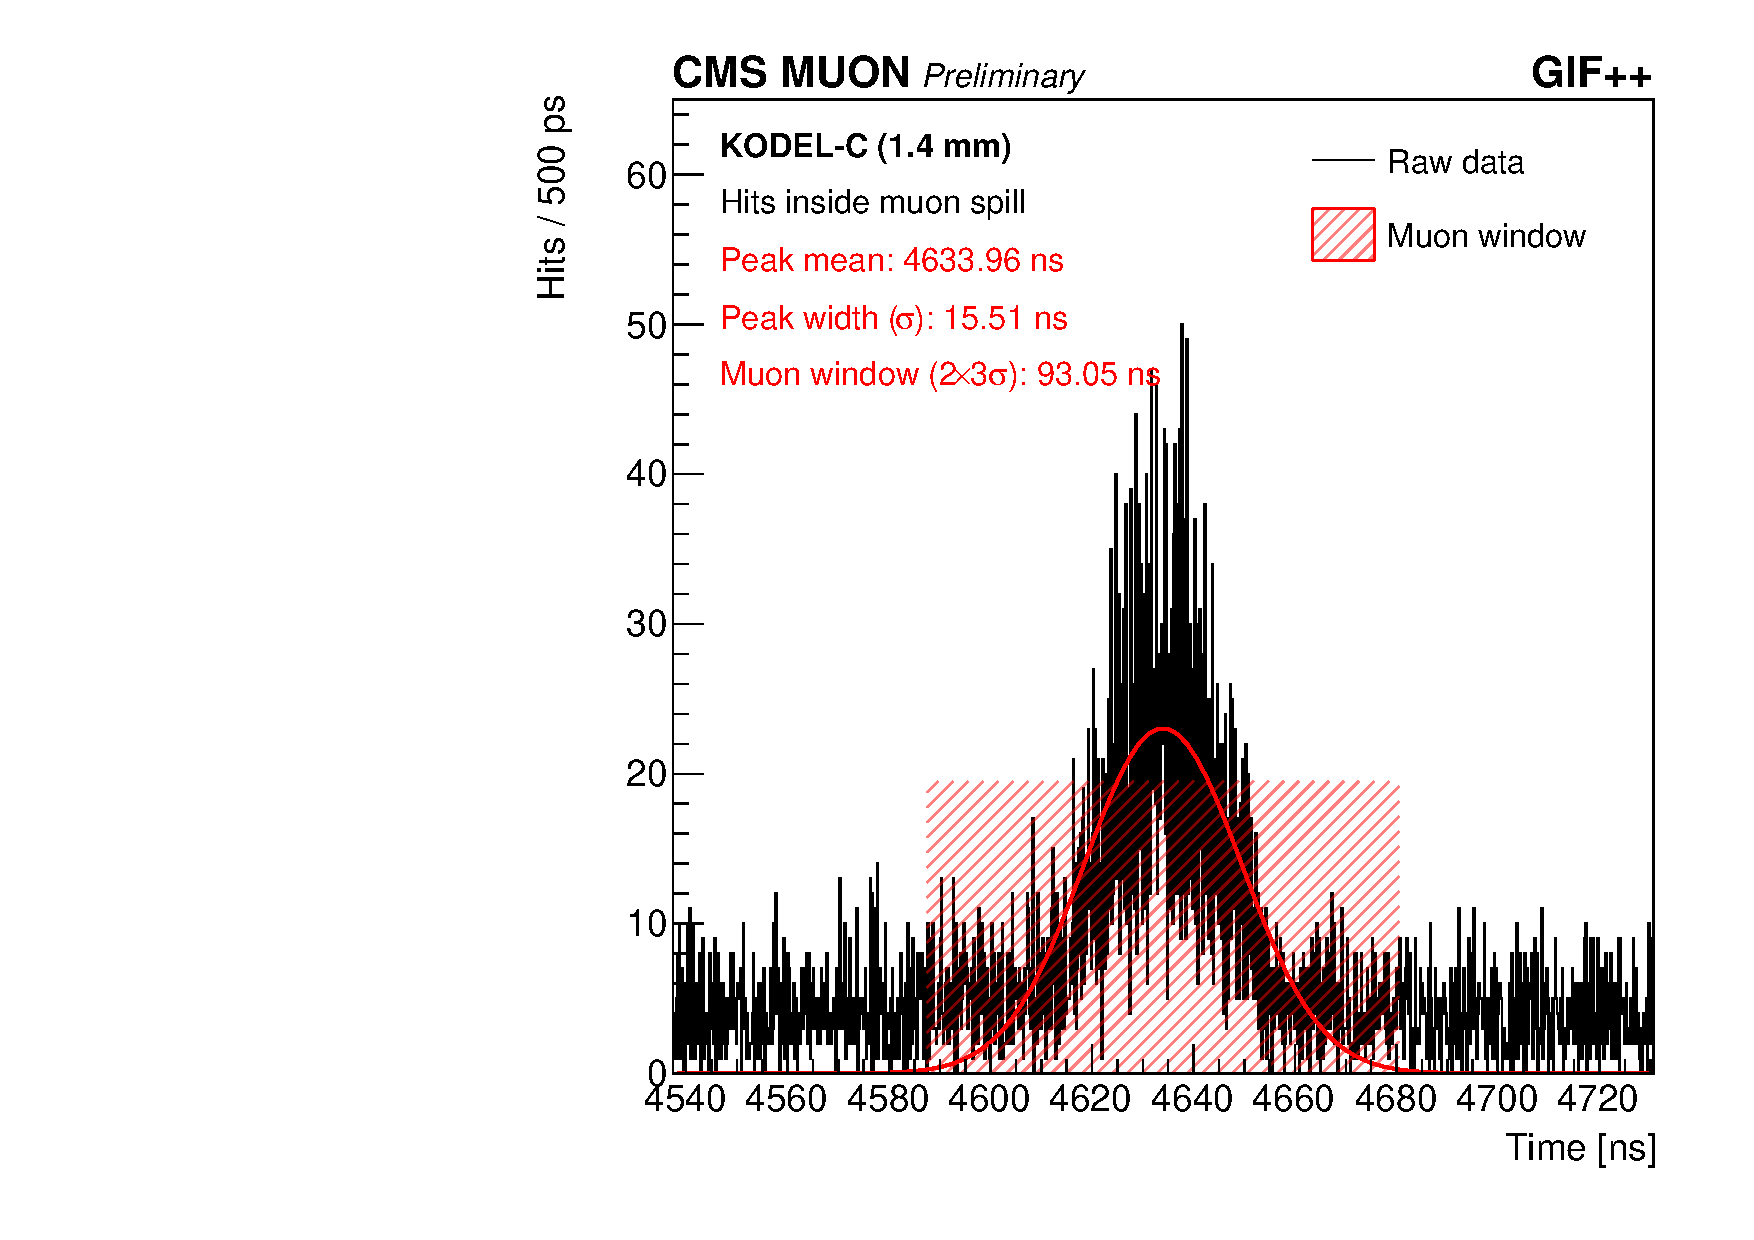
\includegraphics[width=0.45\textwidth]{figures/timeProfile_spill_zoomed.pdf}}}\\
  \legend{Hits recorded from a 1.4 mm double-gap chamber at GIF++. In (a) the is possible to see a narrow peak that comes from the triggered muon beam and a background that comes from gammas in (b) the time profile is zoomed in the muon beam region and a Gaussian fit is done to determine the muon time window.}
\end{figure}

The efficiency is calculated by 
\begin{equation}
    \epsilon_{tot} = N_{tot}/N_{evt},
\end{equation}
where the N$_{tot}$ are the number of events with at least 1 hit inside the muon time window and N$_{evt}$ is the number of recorded events. Still, this is have contamination of gammas that where detected inside the muon time window that. One strategy to remove the gamma contribution to the efficiency is to use the Bayes probability formula for dependent measurements
\begin{eqnarray}
    \epsilon_{tot} = \epsilon_\mu + \epsilon_\gamma - \epsilon_\mu \times \epsilon_\gamma, \nonumber \\ 
    \epsilon_\mu = \frac{\epsilon_{tot} - \epsilon_\gamma}{1-\epsilon_\gamma},
\end{eqnarray}
where $\epsilon_\gamma$ is the fake efficiency from gammas, that can be extracted by calculating the efficiency in a region outside of the muon window. and $\epsilon_\mu$ is the real muon efficiency. This approach was used to measure the muon efficiency for CMS RPC chambers during tests beams in 1997 at the old Gamma Irradiation Facility \cite{Layter:343814}. The gamma efficiency depends on the size of the time window, which is not optimal. Furthermore, for lower photon flux, the fake efficiency calculation can suffer from lower statistics. To have a more reliable efficiency measurements, the tracking system was proposed.

Figure \ref{fig:GIF_setup} shows the experimental setup at GIF++. There are two trolleys, in the one closest to the gamma source the test chamber is placed (from now on refereed to as KODEL-C). On the trolley farther from the gamma source, two tracking RPC chambers are installed (from now on refereed to as GT1 and GT2), with their strip planes oriented perpendicular to each other to allow measurement in two directions. Details on the used chambers characteristics.

\begin{figure}[!htm]{15cm}
\caption{Experimental Setup at GIF++.}%
\label{fig:GIF_setup}
\fbox{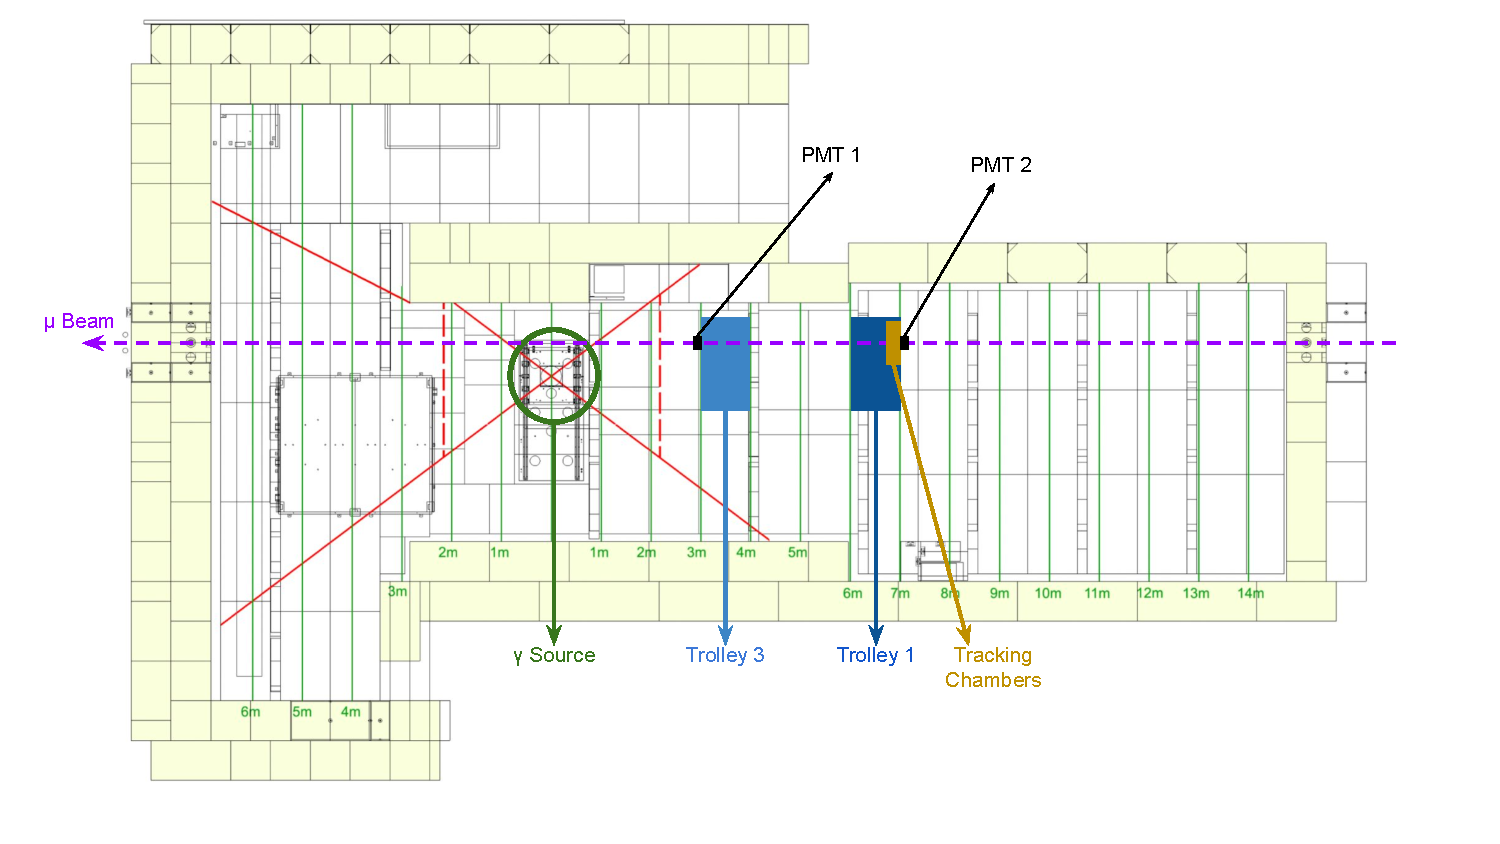
\includegraphics[width=0.7\hsize]{figures/GIF_setup.pdf}}
\legend{The experimental setup inside the GIF++ bunker. There are two trolleys where RPC chambers are placed for irradiation. The tracking chambers are located in the trolley farther from the gamma source.}
\source{\cite{https://doi.org/10.48550/arxiv.2211.16591}}
\end{figure}

\begin{table}[!htbp]{15cm}
\caption{Characteristics of the chambers used in the tracking analysis}\label{tab:RPCchar}
\begin{tabular}{|c|c|c|c|}
    \hline
    Name & Gap type & Strip Plane & Front-End Electronics \\
    \hline
    \multirow{2}{*}{GT1 (tracking)} & Double Gap HPL & 32 strips & CMS Electronics \\ 
     & 2mm thickness & 1.45 cm pitch & 150 fC, 100 ns port width \\
    \hline
    \multirow{2}{*}{GT2 (tracking)} & Double Gap HPL & 32 strips & CMS Electronics \\ 
     & 2mm thickness & 1.45 cm pitch & 150 fC, 100 ns port width \\
    \hline
    \multirow{2}{*}{KODEL-C (test)} & Double Gap HPL & 32 strips & Custom Electronics \\ 
     & 1.4mm thickness & 1.94 cm pitch & 75 fC, 60 ns port width \\
    \hline
\end{tabular}
\legend{Characteristics of the chambers used for the tracking and the test chamber to evaluate the performance of the algorithm}
\source{\cite{https://doi.org/10.48550/arxiv.2211.16591}}
\end{table}

To start the tracking analysis first the events are chosen so that at least there is at least one hit inside the muon time window for the two tracking chambers. This is required so that the the probability of hits from background or tracking is very low. A 2D hit profile is constructed to check the alignment of the tracking chambers and the muon beam (Fig. \ref{fig:2D_hit_profile}). the tracking chambers position in the trolley is adjusted so that the muon beam is centred in the run, this way we can avoid the muons to fall out of the detecting region by possible beam adjustments during the data taking. 

\begin{figure}[!htm]{15cm}
\caption{2D hit profile of tracking chambers at GIF++.}%
\label{fig:2D_hit_profile}
\fbox{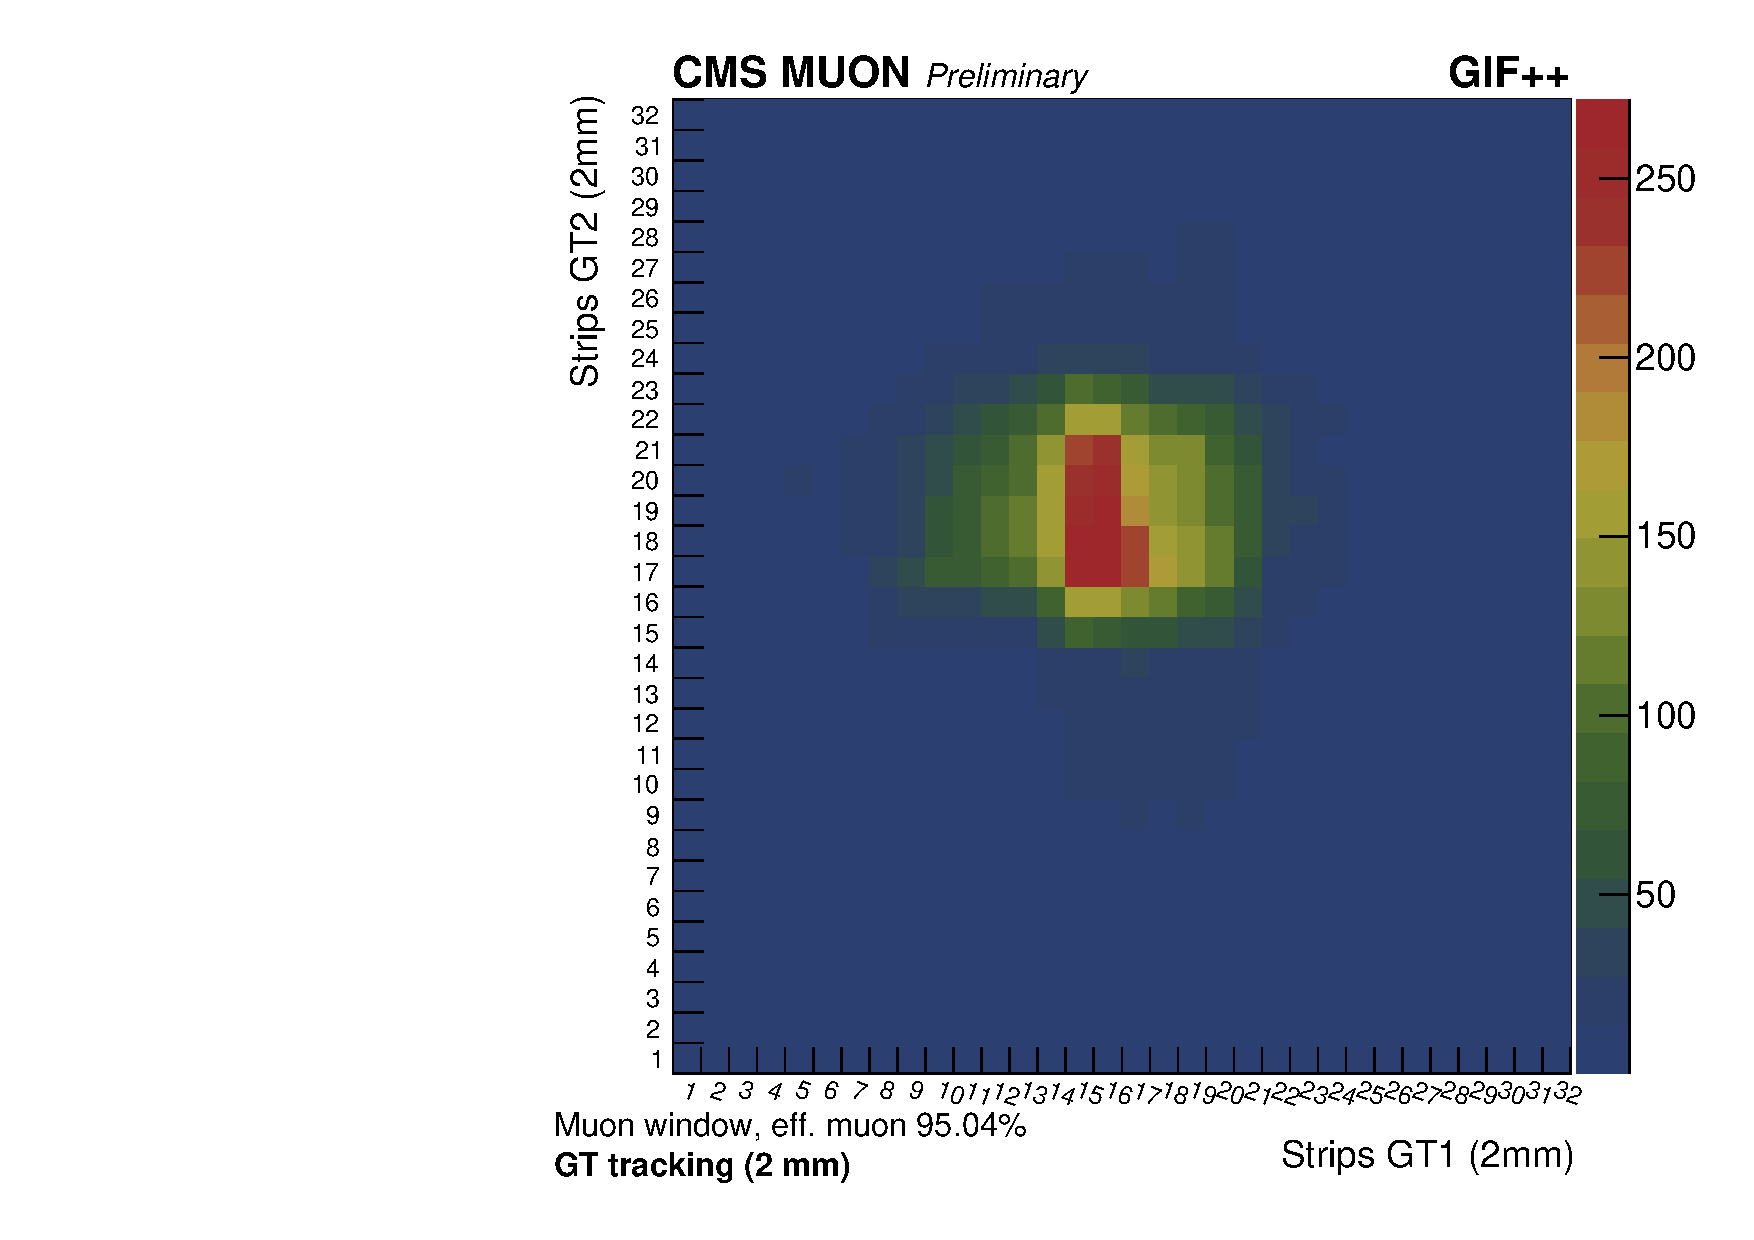
\includegraphics[width=0.7\hsize]{figures/muonHitProfile.pdf}}
\legend{2D hit profile from the tracking chambers at GIF++. The chambers' strip plane are oriented perpendicularly to each other so that it is possible to make a 2D hit mapping.}
\source{\cite{https://doi.org/10.48550/arxiv.2211.16591}}
\end{figure}

The tracking algorithm relies on the assumption that the beam is perpendicular to the strip plane, therefore it is only needed to extrapolate the position of the hit from the tracking to the test chamber and check for a matching hit. For every event, the following steps are taken \cite{https://doi.org/10.48550/arxiv.2211.16591}:
\begin{enumerate}
    \item Perform the clusterization of the hits in the tracking chambers, where events with more than one cluster are rejected. The cluster barycenters are defined as the mean position in the cluster;
    \item Perform the clusterization for the test chambers and calculate the clusters' barycenters;
    \item Form a perpendicular track starting from the tracking cluster barycenter;
    \item Check for a match in any cluster on the test chamber. 
\end{enumerate}

The clusterization is done by grouping hits that are adjacent and does not exceed a difference of time. The difference of time is previously determined in cosmic or source off data taking and depends on the chambers and front-end electronics and DAQ used. The cluster barycenter is defined as the geometrical mean position of the cluster. Figure \ref{fig:tracking_evt} shows an example of a event where a matching hit was found.

\begin{figure}[!htm]{15cm}
\caption{2D hit profile of tracking chambers at GIF++.}%
\label{fig:tracking_evt}
\fbox{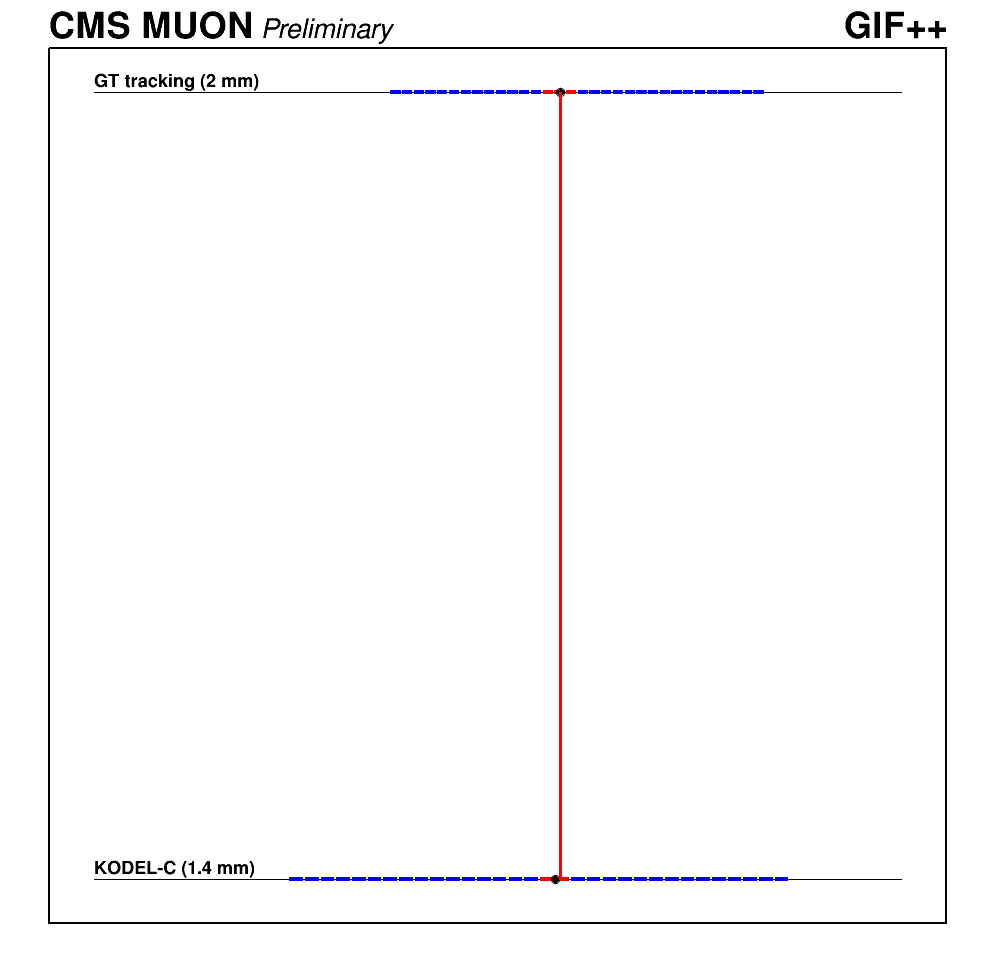
\includegraphics[width=0.5\hsize]{figures/event_0.png}}
\legend{Example of one event in which the hit on tracking chamber was matched on the test chamber. The strips in red represent the hits and the point in black is the 
cluster barycentre.}
\source{\cite{https://doi.org/10.48550/arxiv.2211.16591}}
\end{figure}

Efficiency curves of the test chambers were used to evaluate the validity of the tracking in rejecting the fake hits caused by the gammas. On Fig. \ref{fig:effcomparison} the efficiency curves are compared for three gamma background conditions. There are three curves in each plot. The black curve is calculated without the tracking, taking into consideration all the hits in the muon time window. For the blue one, only the hits that passed the tracking criteria were considered. Finally, for the red curve, the HV was recalculated to remove the voltage drop caused by the resistance of the electrodes using the Ohm law
\begin{equation}
    HV_{gas} = HV_{app} - R \cdot I,
\end{equation}
where HV$_gas$ is the corrected HV, HV$_app$ is the applied HV, R is the resistance of the electrode, determined previously by argon scans \cite{peskov2018resistive}. This correction decouples the shift to the right of the curve on higher cluster rates, caused by the increase of the current. Therefore, HV$_{gas}$ is the effective HV applied to the gas volume. 

\begin{figure}[!htm]{15cm}
  \caption{Comparison of the tracking algorithm using efficiency curves.} 
  \label{fig:effcomparison}
  \subfloat[][]{\label{subfig:ABSOFF}%
    \fbox{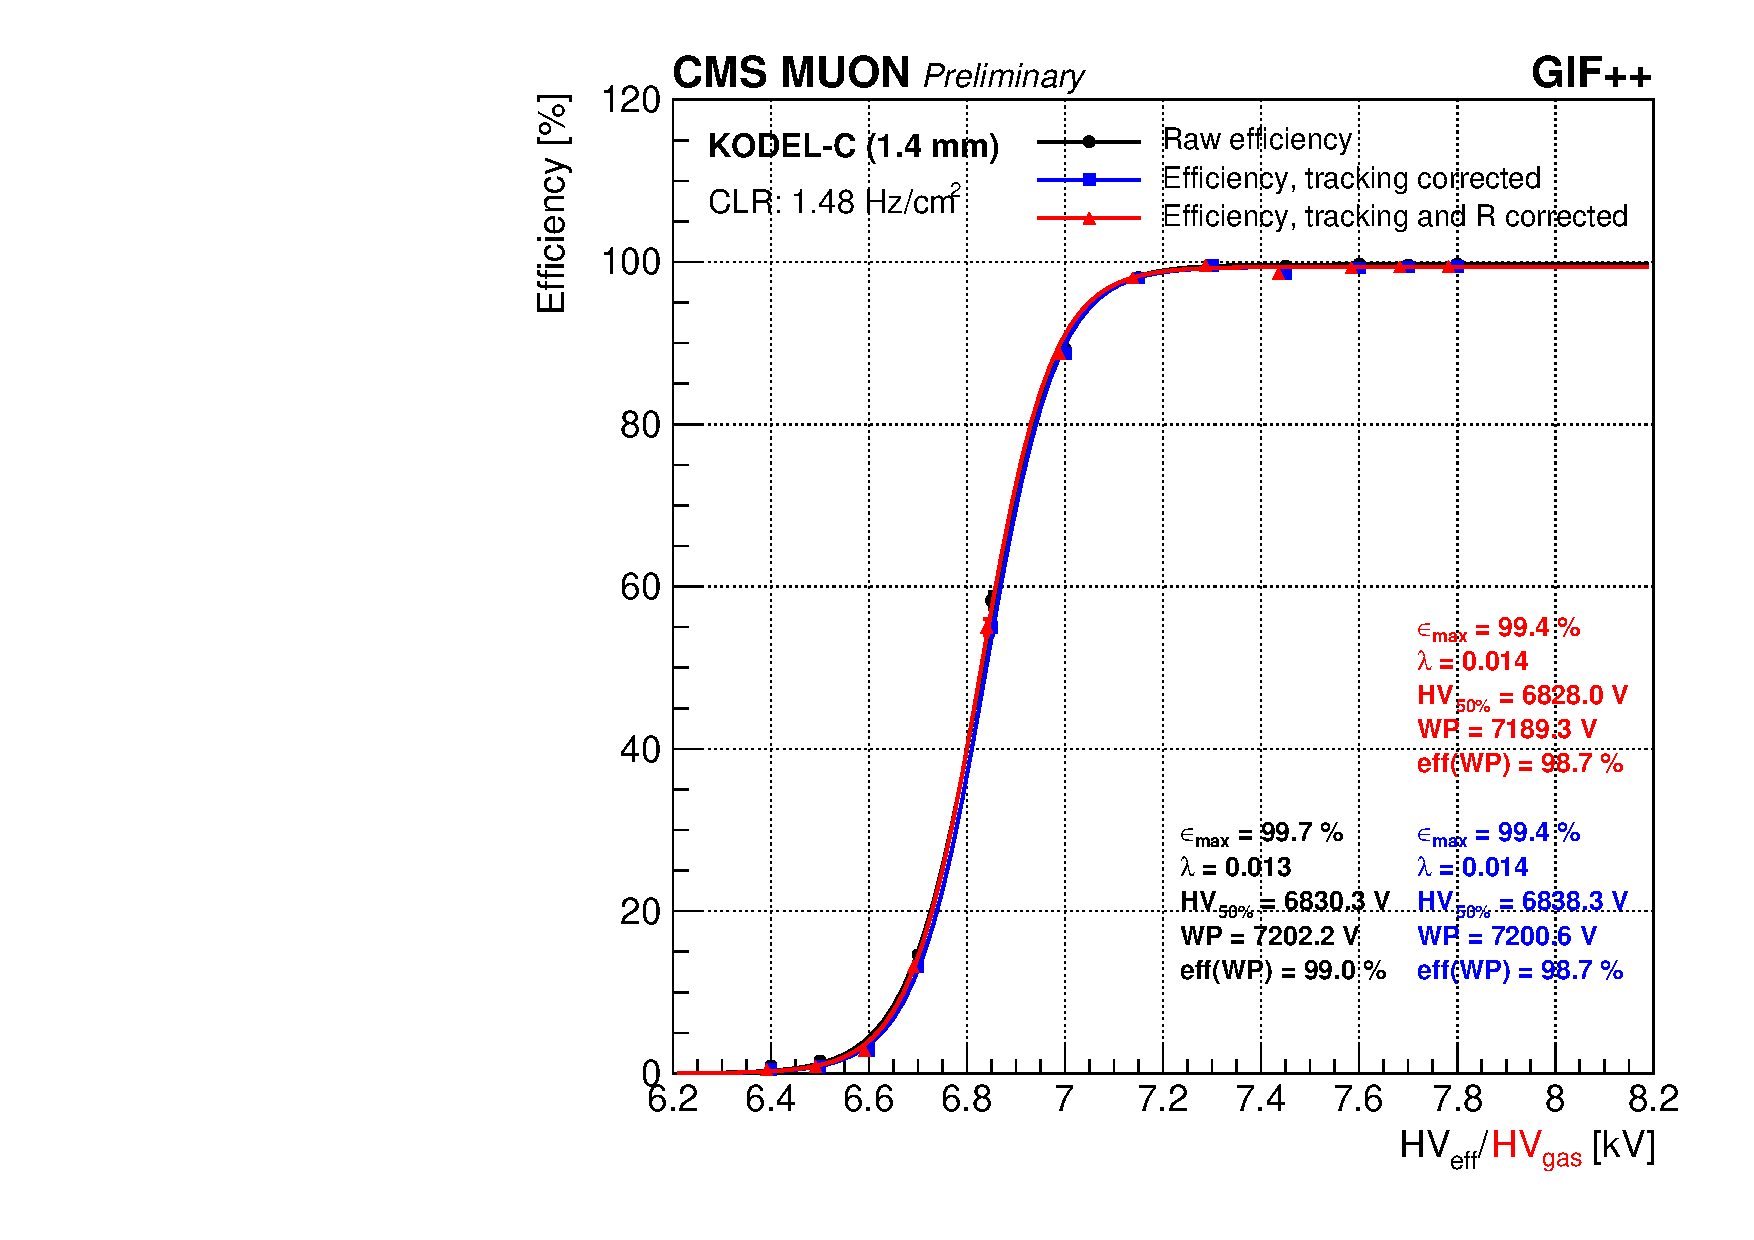
\includegraphics[width=0.45\textwidth]{figures/all_ABS_OFF.pdf}}}\hfill
  \subfloat[][]{\label{subfig:ABS10}%
    \fbox{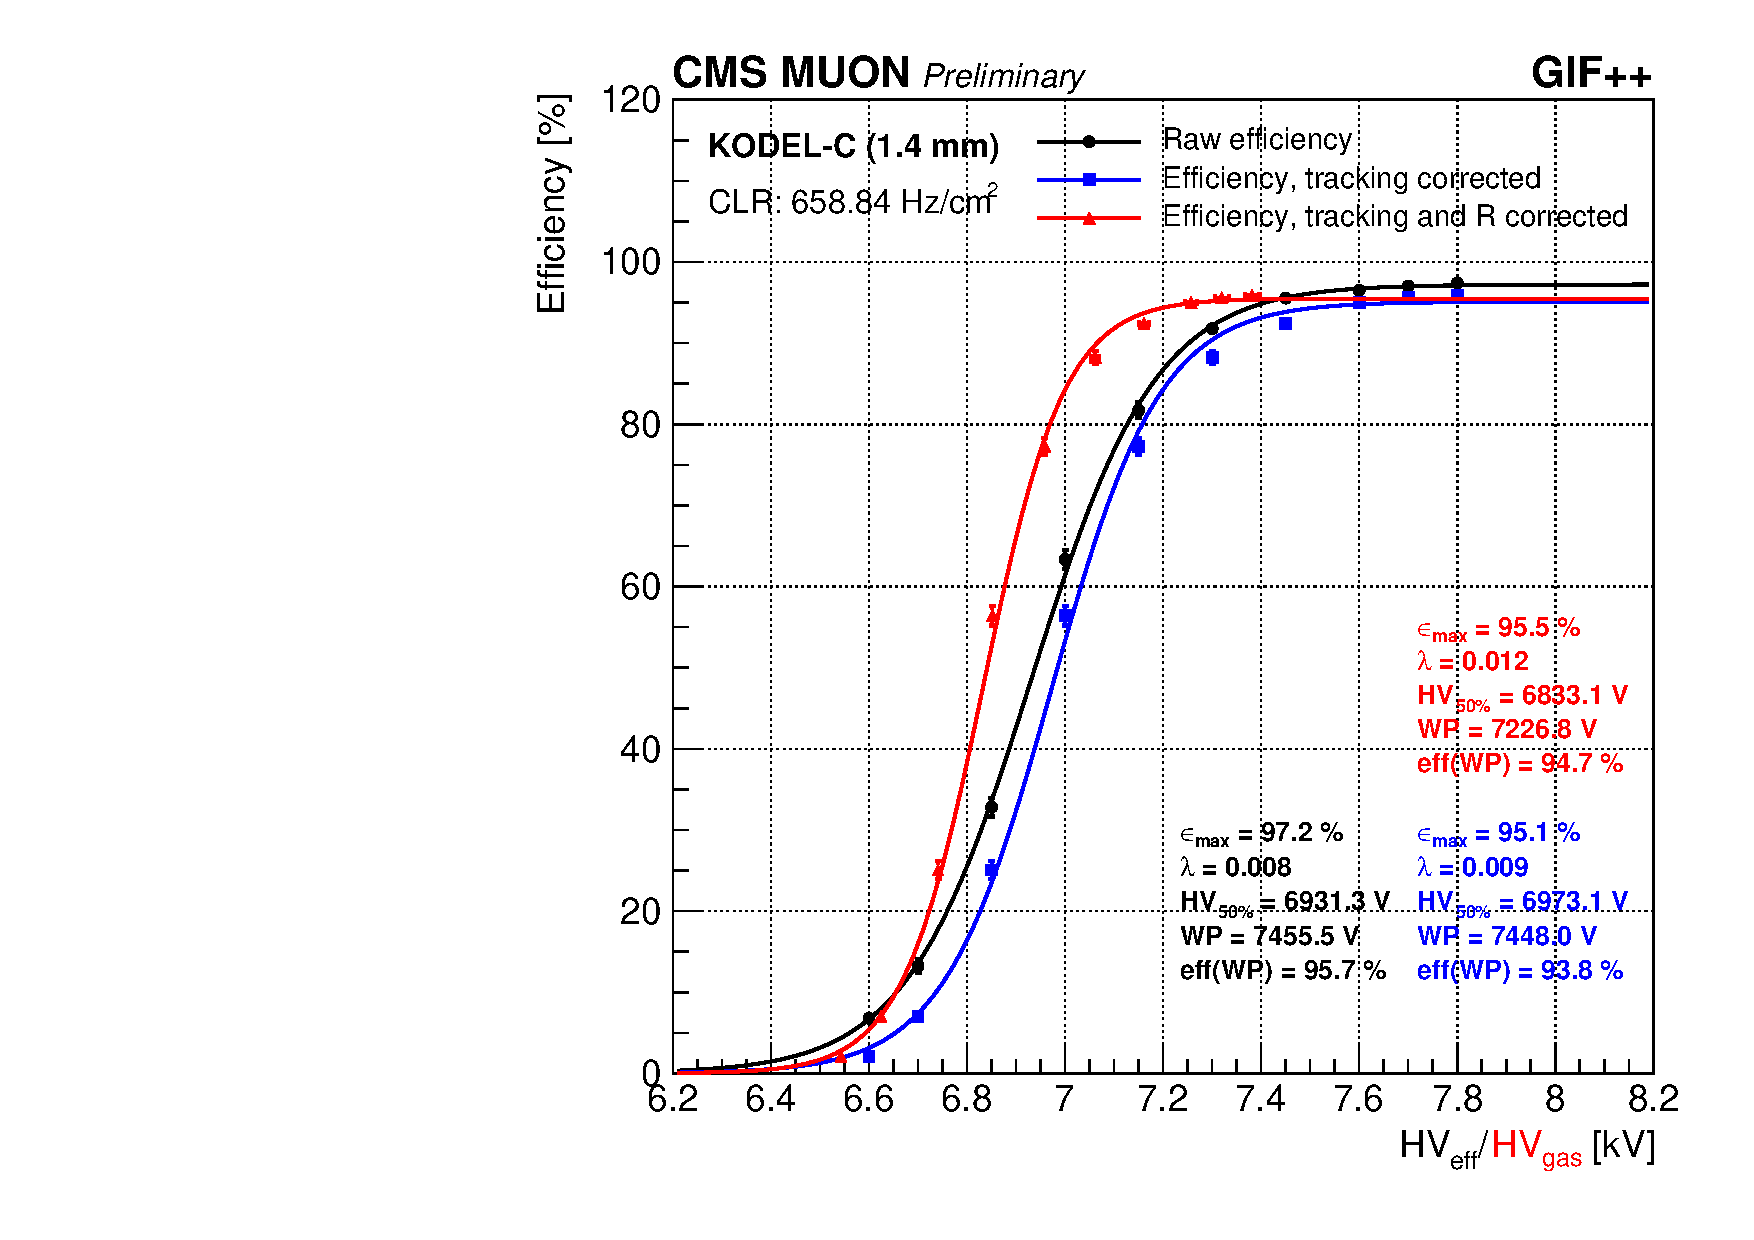
\includegraphics[width=0.45\textwidth]{figures/all_ABS_10.pdf}}}
    \hfill
  \subfloat[][]{\label{subfig:ABS3p3}%
    \fbox{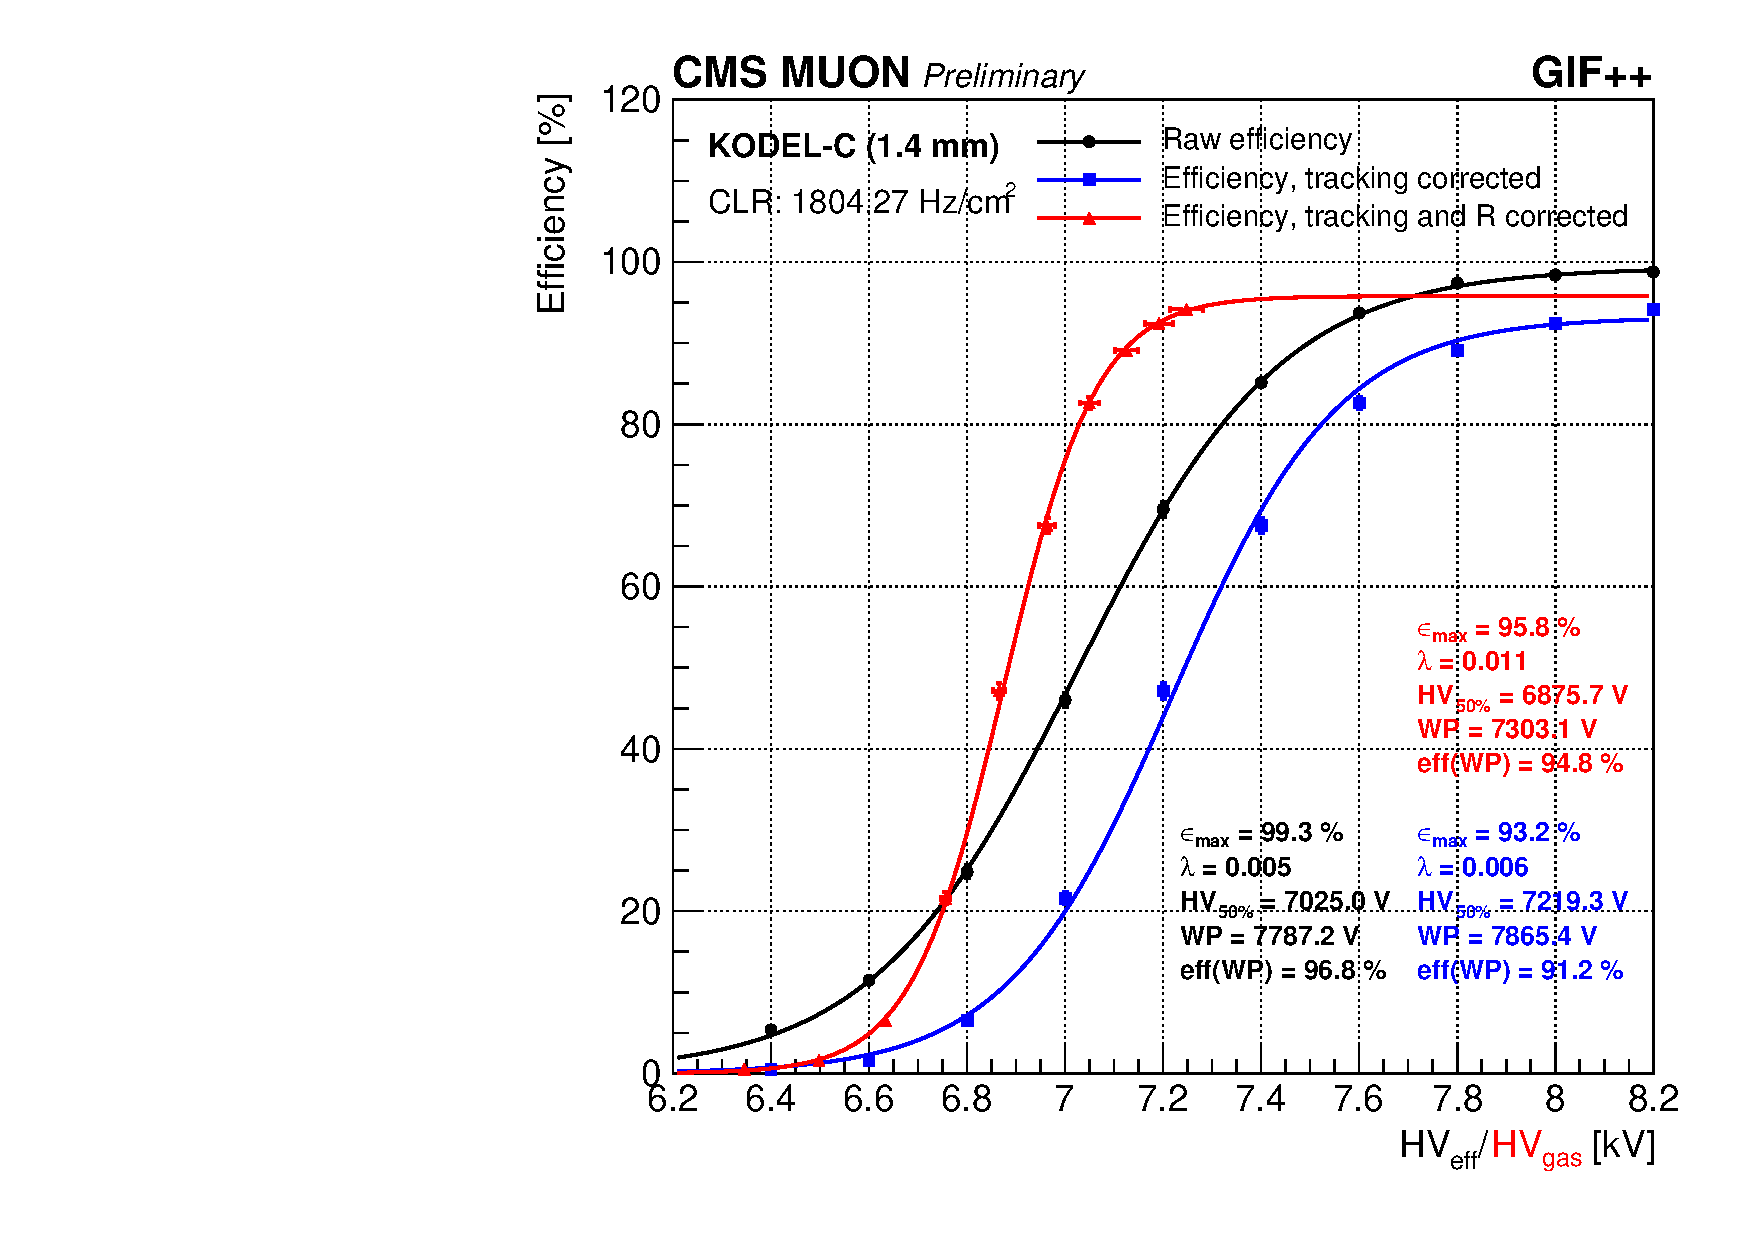
\includegraphics[width=0.45\textwidth]{figures/all_ABS_3p3.pdf}}}\\
  \legend{Efficiencies and their sigmoid fits measured at three photon fluxes with measured at the working-point high voltages gamma cluster rates of 1.804 kHz (a), 0.645 kHz (b), and 1.48 Hz (c), respectively. The curve in black is the efficiency calculated with all hits inside the muon window, the blue one is with applied tracking correction and the one in red -- with tracking and resistance correction.}
  \source{\cite{https://doi.org/10.48550/arxiv.2211.16591}}
\end{figure}

In Fig. \ref{subfig:ABSOFF} the curves are equivalent, this behavior is expected, since at lower rates, the currents are low, so there are no fake hits nor HV correction. In Figure \ref{subfig:ABS10}, the background rate becomes substantial, so we can see a shift to the right in the curves without resistance correction, caused by the aforementioned voltage drop, which is much more noticeable in Fig. \ref{subfig:ABS10}. A decrease of the maximum efficiency with the increase of rate is expected, because of the dead time of the front-end electronics, but we can see an increase in the raw efficiency, which indicates a high fake hit contamination.

To finalize the discussion, the plots of the efficiency curves with tracking and with tracking and resistance correction can be seen in Fig. \ref{fig:eff_curves}. The effect of the voltage drop on the electrodes is very noticeable in Fig. \ref{subfig:sigmoids_trk} and it is also possible to see the expected decrease maximum efficiency, proving that the fake hit contamination was removed using the tracking. In Fig. \ref{subfig:sigmoids_trk_corr} it is still possible to see a shift to the right in the curves, this is also expected, since the high rates induce an efficiency drop in the RPCs, because of the reduce of the gas amplification caused by the space charge effect \cite{Lippmann:2003yb}. 

\begin{figure}[!htm]{15cm}
  \caption{Efficiency curves for various gamma background rates.} 
  \label{fig:eff_curves}
  \subfloat[][]{\label{subfig:sigmoids_trk}%
    \fbox{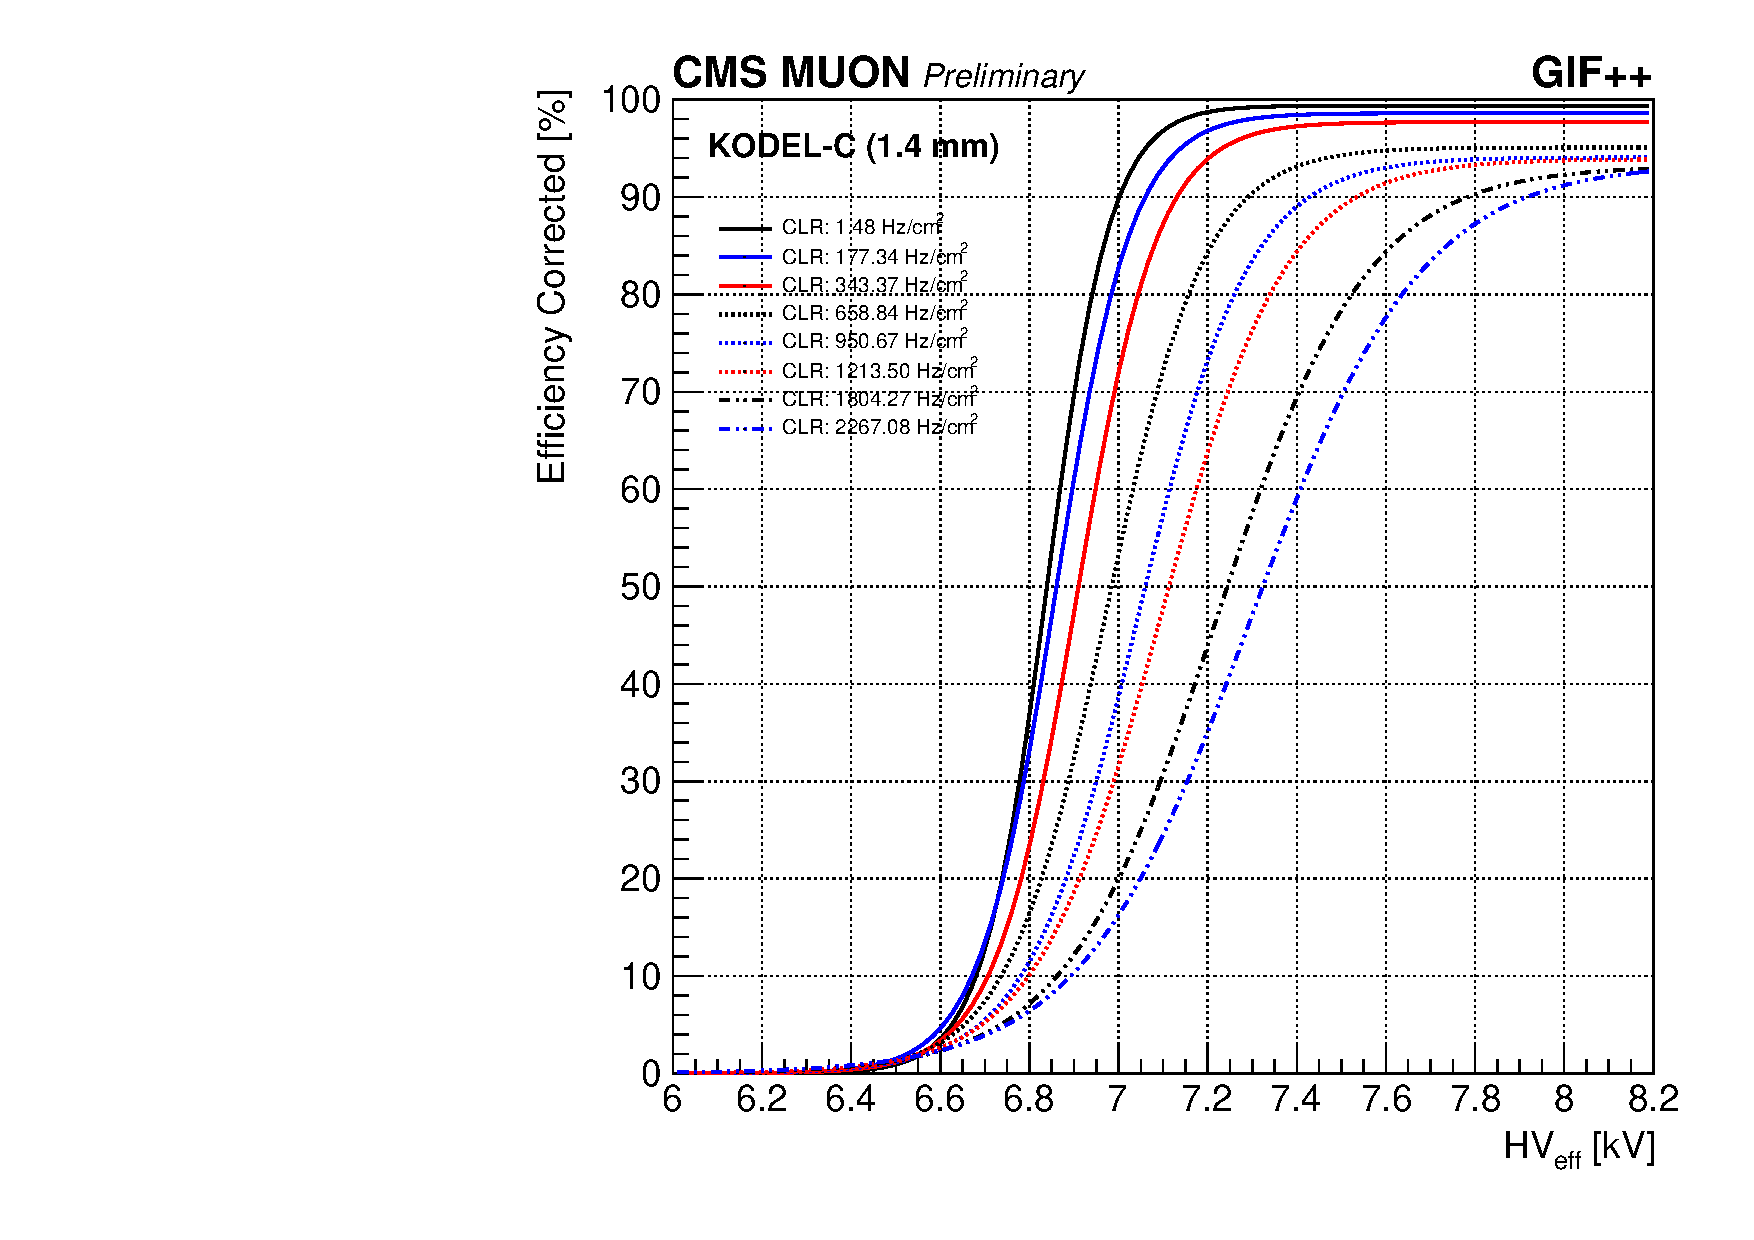
\includegraphics[width=0.45\textwidth]{figures/sigmoids_trk.pdf}}}\hfill
  \subfloat[][]{\label{subfig:sigmoids_trk_corr}%
    \fbox{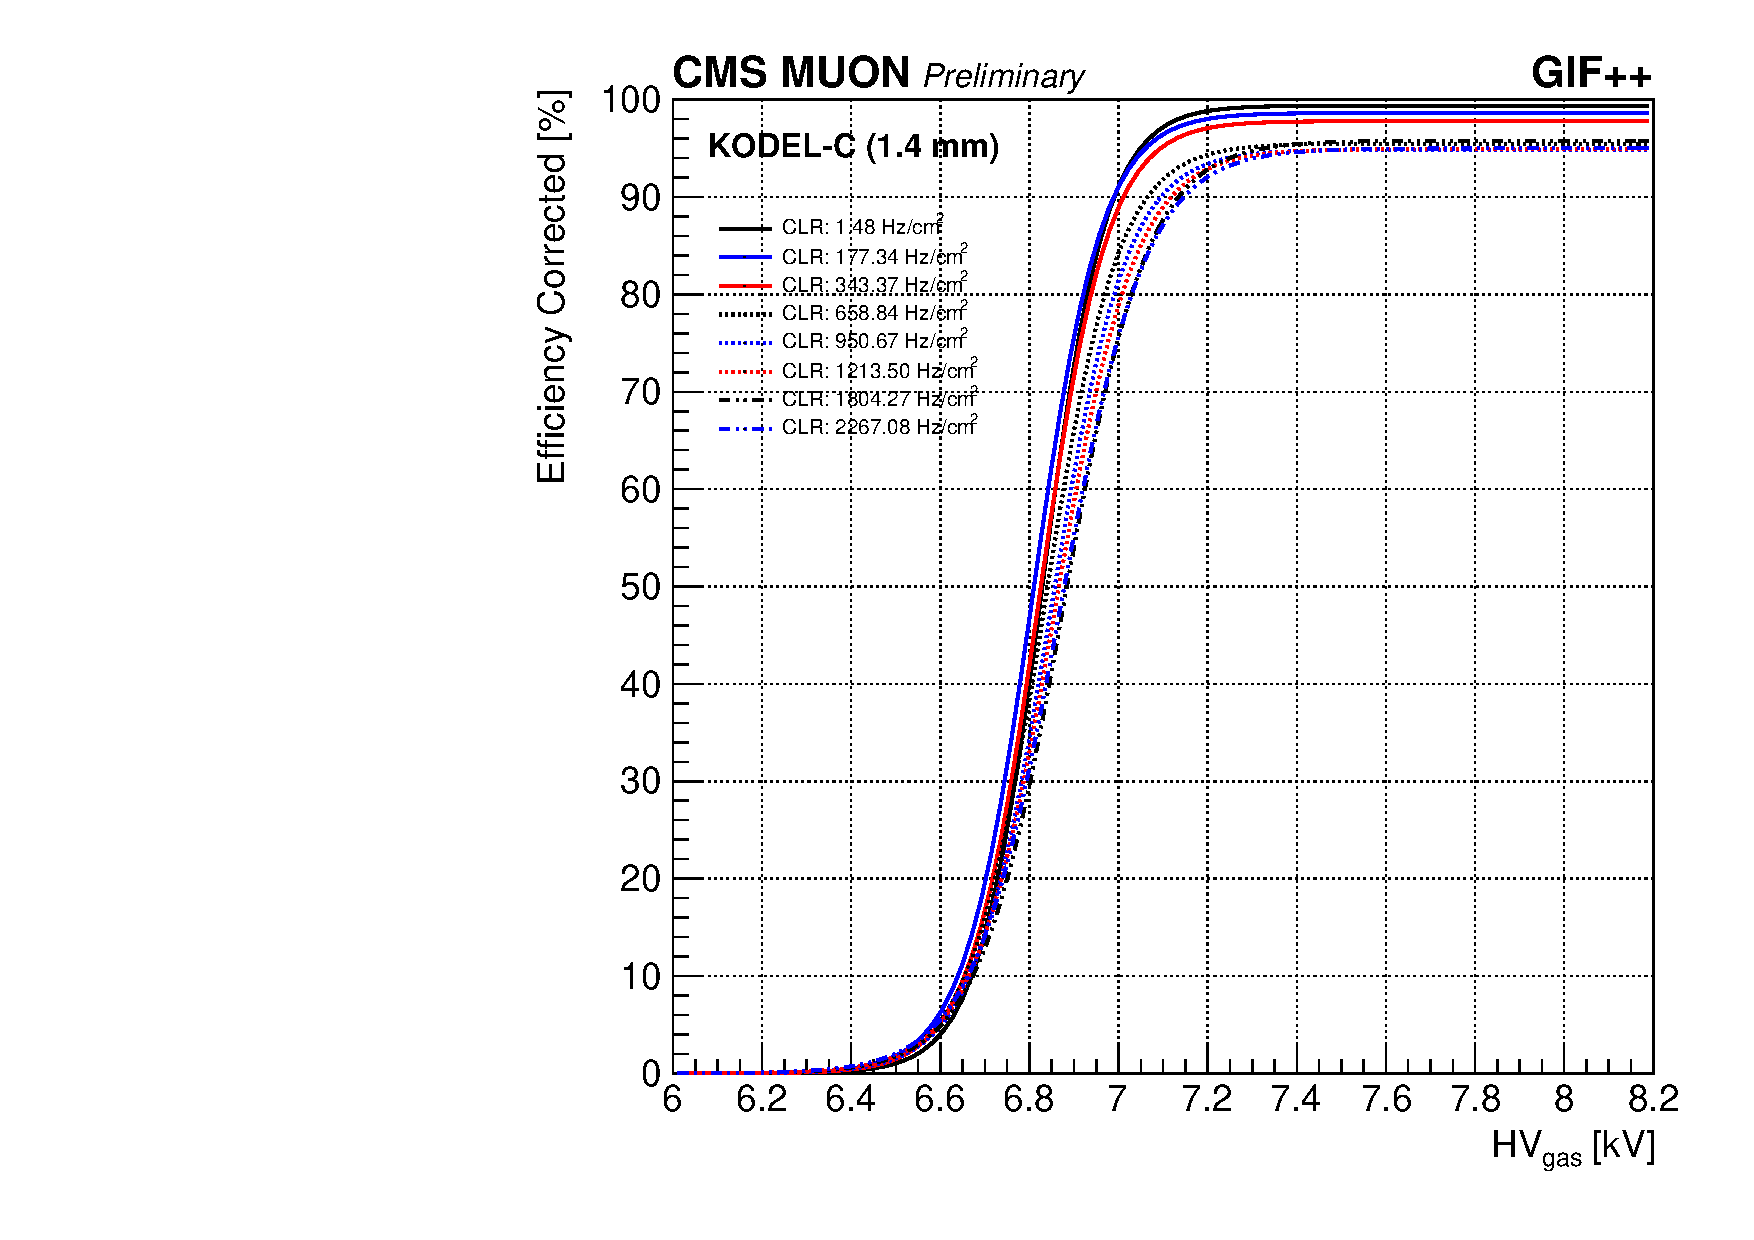
\includegraphics[width=0.45\textwidth]{figures/sigmoids_trk_corr.pdf}}}\\
  \legend{Efficiency curves for various gamma background rates. In (a) the HV applied is corrected only by pressure and temperature (HV$_{eff}$), while in (b) the HV is also corrected by the resistance of the gaps (HV$_{gas}$).}
  \source{\cite{https://doi.org/10.48550/arxiv.2211.16591}}
\end{figure}

The tracking system implementation at GIF++ was successful, and was able to remove the fake hit contribution. The KODEL-C is a prototype used to evaluate the performance of the 1.4 mm gaps, the same used in the iRPC design. It showed good results in the high rate environment, even at rates higher than 2 kHz/cm$^2$, with increase on the working point of $\approx$650 V with efficiency loss of $\approx$ 7.5\%, using a custom front-end. The iRPC front-end design have lower threshold and dead time so it is expected to perform better \cite{CMS:2021bxv}.
\chapter{Physics Analysis}
%================================================================

This chapter will discuss about the cross section measurement of the associated production of $\Upsilon$ and $D^{*\pm}$ using the full CMS Run 2 data with 13 TeV center-of-mass energy. \textcolor{red}{falar mais}

\section{Datasets and Simulation}
\subsection{Data Samples}

The data samples were recorded by the CMS detector during the LHC Run 2 in 2016-2018 at a center-of-mass energy of 13 TeV and are composed only by events certified as good for physics analysis. The Table \ref{tab:datasamples} displays all the data samples used. The total recorded luminosity of all data samples is 137.61 fb$^{-1}$.

\begin{table}[!htbp]{15cm}
  \caption{Data samples considered in this work}\label{tab:datasamples}
  \begin{tabular}{ c }
    Dataset \\ 
    \hline
    /MuOnia/Run2016B-21Feb2020\_ver1\_UL2016\_HIPM-v1/AOD \\
    /MuOnia/Run2016B-21Feb2020\_ver2\_UL2016\_HIPM-v1/AOD \\
    /MuOnia/Run2016C-21Feb2020\_UL2016\_HIPM-v1/AOD \\
    /MuOnia/Run2016D-21Feb2020\_UL2016\_HIPM-v1/AOD \\
    /MuOnia/Run2016E-21Feb2020\_UL2016\_HIPM-v1/AOD \\
    /MuOnia/Run2016F-21Feb2020\_UL2016\_HIPM-v1/AOD \\
    \hline
    /MuOnia/Run2016F-21Feb2020\_UL2016-v1/AOD \\
    /MuOnia/Run2016G-21Feb2020\_UL2016-v1/AOD \\
    /MuOnia/Run2016H-21Feb2020\_UL2016-v1/AOD \\
    \hline
    /MuOnia/Run2017B-09Aug2019\_UL2017-v1/AOD \\
    /MuOnia/Run2017C-09Aug2019\_UL2017-v1/AOD \\
    /MuOnia/Run2017D-09Aug2019\_UL2017-v1/AOD \\
    /MuOnia/Run2017E-09Aug2019\_UL2017-v1/AOD \\
    /MuOnia/Run2017F-09Aug2019\_UL2017-v1/AOD \\
    \hline
    /MuOnia/Run2018A-12Nov2019\_UL2018-v1/AOD \\
    /MuOnia/Run2018B-12Nov2019\_UL2018-v1/AOD \\
    /MuOnia/Run2018C-12Nov2019\_UL2018-v1/AOD \\
    /MuOnia/Run2018D-12Nov2019\_UL2018-v1/AOD \\
  \end{tabular}
  \legend{Data Samples used in the analysis corresponding to the full CMS Run 2 data taking.}
\end{table}

From the analysis point view, data samples are divided into four subsamples (2016APV, 2016, 2017 and 2018), to take into account the differences in the detector in the course of Run 2 (e.g. lose in the efficiency due to aging and installation of new detectors).

\subsection{Simulation Samples}

The simulation samples are done via Monte Carlo (MC) simulation, where the MC method is used in programs to model the physics processes. The starting point of the simulation is the event generation, where the events following a set of physics processes of interest are created by the MC generator.

First, the parton level matrix element of the process is calculated perturbatively up to a fixed order. After, the parton showering is done to take into account the higher order effects, such as initial and final state radiation (ISR and FSR). This is followed by the hadronization, where the quarks and gluons form the quarks. Finally, the simulation should also handle the particles decay.

The detector simulation follows the event generation. Here, the interaction of the generated particles with the detector is simulated. In CMS, the detector response is simulated using \textsc{Geant4} \cite{GEANT4:2002zbu}. The simulated detector response pass through the same processing chain as the real data forming the final simulated sample.

The MC samples were used in this analysis to simulate the two components of the signal, the SPS and DPS. The only background was not simulated, since it is only combinatorial

The DPS was created using the \textsc{Pythia8} \cite{Sjostrand:2014zea} as event generator, parton showering and for hadronization. For the decays of the heavy flavour hadrons, \textsc{EvtGen} \cite{Lange:2001uf} was used. The SPS sample is similar to the DPS, with the addition of the \textsc{HELAC-Onia} \cite{Shao:2012iz, Shao:2015vga}, which was used for event generation.

In the same way as the data, the MC samples are divided into subsamples to take into account the detector differences in the course of Run 2. The detector simulation is tunned to better represent the detector conditions in each subsample.

\textcolor{red}{colocar imagens da simulação}

\section{\texorpdfstring{$\Upsilon$ + D$^{*\pm}$}{Y+D*} Reconstruction}

The $\Upsilon$ + D$^*$ reconstruction is done from the reconstructed tracks in an event. As shown in Fig. \ref{fig:drawing_event}, there are five different particles in the final state an event - three coming from D$^*$ and two from $\Upsilon$. The D$^*$ have a low combinatorial background when compared with other open charm mesons because of it very characteristic signature - very small difference of mass between D$^*$ and D$^0$ restricting the phase space of the slow pion. Also, the kaon and pion can be identified even without a particle identification detector, since it should have a opposite charge to the slow pion, removing the ambiguity of the D$^0$ reconstruction.

\begin{figure}[!htm]{15cm}
\caption{Drawing of an event of associated production of $\Upsilon$ and D$^{*+}$}%
\label{fig:drawing_event}
\fbox{
\begin{tikzpicture}
  \coordinate (PV) at ( 0,0);
  \coordinate (SV) at ( 2.0,1.8);
  \coordinate (BL) at (-3,0);
  \coordinate (BR) at ( 4,0);

  \draw[beamcol,dashed,name path=beam]
    (BL) -- (BR);
  \draw[SVcol,dashed]
    (PV) -- (SV)
    node[midway,above=0.1,left=0.1] {$D^0$};

  \draw[->,mygreen,line width=1]
    (SV) to[bend right] (1.0,3.0) node[above right] {$\pi^+$};
  \draw[->,mygreen,line width=1]
    (SV) to[bend left] (3.0,3.0) node[above left] {$K^-$};

  \draw[->,red,line width=1]
    (PV) to[bend right=20] (-2.0,1.0) node[below right] {$\mu^+$};
  \draw[->,red,line width=1]
    (PV) to[bend left=20] (-1.0,2.0) node[below left] {$\mu^-$};


  \draw[->,SVcol,line width=1]
    (PV) arc[start angle=150, end angle=0, radius=0.5] node[below right] {$\pi_s^+$};
  
  \fill[beamcol]
    (PV) ellipse (9pt and 4.5pt)
    node[beamcol!95!black,below left] {PV $\color{red}{\Upsilon} \color{beamcol}{+} \color{SVcol}{D^*}$};
  \fill[SVcol]
    (SV) circle (4pt) node[below right] {SV};
\end{tikzpicture}
}
\legend{Drawing of an event of associated production of $\Upsilon$ and D$^*$. $\Upsilon$ decays into two opposite charge muons, while D$^{*+}$ decays into a pion and D$^0$, which later decays into a kaon and a pion.}
\end{figure}

The D$^*$ reconstruction starts by finding a suitable D$^0$ candidate. For this, two tracks of opposite charge are paired to check whether they form a common vertex using the Kalman Filter method \cite{Fruhwirth:1991pm, Speer:927395}. If the fit is valid and its p-value is greater than 1\%, the D$^0$ candidate is selected. The vertex determination also allows for a better calculation of the kinematic variables of the tracks and it is called secondary vertex (SV).

A primary vertex (PV) is assigned to the D$^0$ candidate as the one closest to the SV in order to calculate the decay length, defined as
\begin{equation}
    dl = \frac{|\Vec{p}_{D^0} \cdot \Delta\Vec{l}|}{|\Vec{p}_{D^0}|},
\end{equation}
where $\Vec{p}_{D^0}$ is the D$^0$ trimomentum and $\Delta\Vec{l}$ is the distance between the PV and SV, the decay length significance is very important because it can be used to filter a lot of background, it is defined as
\begin{equation}
    dl_{sig} = \frac{dl}{dl_{err}},
\end{equation}
where $dl_{err}$ is the uncertainty of $dl$. Finally, another important variable is the cosine of the angle between the PV and SV position vectors (pointing angle)
\begin{equation}
    \cos{\alpha} = \frac{dl}{\Delta\Vec{l}} \; ,
\end{equation}
which hints the alignment between the PV and the SV.

After the D$^0$ candidates is reconstructed, a new track coming from the same PV of the D$^0$ is added to form the D$^*$ candidate and its momentum resolution is improved by adding the PV to the track fit.

The $\Upsilon(nS)$ reconstruction is done in a similar way to the D$^0$. Two muons with opposite charge are selected and its vertex is determined from the fit. If the vertex is valid and has a p-value greater than 1\% we have a dimuon candidate. The invariant mass of the dimuon should be in the range of $8.5 < m_{\mu\mu} < 11.5$ GeV in order to be classified as a $\Upsilon(nS)$ candidate. 

Finally, in order to pair the $\Upsilon(nS)$ and the $D^*$, a vertex fit of the two muons and the slow pion is performed. If valid, the vertex p-value is determined.

In this stage of the reconstruction, very loose cuts are applied to the candidates, those are specified in the Sec. \ref{subsec:preselcuts}.

\section{Event Selection}\label{sec:evtsel}

\subsection{Preselection Cuts} \label{subsec:preselcuts}

Preselection cuts are used to mitigate some of the combinatorial background and save disk space when recording the NTuple. They are very loose and are further improved when the analysis final cuts are applied (Sec. \ref{sec:selcuts}). The preselection cuts both for the $\Upsilon$ and the D$^*$ candidates are summarized in the Tab. \ref{tab:preselectioncuts}.

\begin{table}[!htbp]{15cm}
  \caption{Preselection cuts.}
  \begin{tabular}{ l | l }
    \hline
    \multicolumn{1}{c|}{Variable} & \multicolumn{1}{|c}{Cut} \\ \hline
    \multicolumn{2}{c}{D$^*$ candidate} \\ \hline
    Transverse momentum of $K$ and $\pi$ ($p_T^{K, \pi}$) & $> 0.3$ GeV \\ \hline
    Transverse and longitudinal impact parameter & \multirow[c]{2}{*}{$< 0.5$ cm} \\ 
    of $K$ and $\pi$ track ($d_{xy}$ and $d_z$) & \\ \hline
    Transverse and longitudinal impact parameter & \multirow[c]{2}{*}{$< 2$ cm} \\ 
    of $\pi_s$ track ($d_{xy}$ and $d_z$) & \\ \hline
    Longitudinal distance between D$^0$ vertex and PV & $< 2$ cm \\ \hline
    Transverse momentum of D$^0$ ($p_T^{D^0}$) & $> 0.9$ GeV \\ \hline
    D$^0$ of D$^{*\pm}$ mass cut ($m_{D^0}$) & $1.5 < m_{D^0} < 2.3$ GeV \\ \hline
    Mass difference between D$^{*\pm}$ and D$^0$ ($\Delta m$) & $< 0.17$ GeV \\ \hline
    $D^0$ candidate vertex probability & $> 0.01$ \\ \hline

    \multicolumn{2}{c}{$\Upsilon$ candidate} \\ \hline
    Pseudorapidity separation between the two $\mu$ ($\Delta\eta_{\mu^+\mu^-}$) & $< 3.0$ \\ \hline
    Transverse and longitudinal impact parameter & \multirow[c]{2}{*}{$< 0.5$ cm} \\ 
    of the two $\mu$ tracks & \\ \hline
    Longitudinal distance between the dimuon & \multirow[c]{2}{*}{$< 0.5$ cm} \\ 
    candidate vertex and the PV & \\ \hline
    Dimuon candidate vertex probability & $> 0.01$ \\ \hline
    Dimuon mass range & $8.5 < m_{\mu\mu} < 11.5$ GeV \\ \hline
  \end{tabular}
  \legend{Preselection cuts used to save disk space when saving the NTuples.}
  \label{tab:preselectioncuts}
\end{table}

\textcolor{red}{colocar imagens da pre seleção?}

\subsection{Trigger}\label{sec:trigger}

The trigger strategy chosen was to use the HLT Paths that filters dimuons, it was required that the trigger had the maximum possible rapidity coverage, to use for discrimination between DPS and SPS, and lower $p_T$ threshold. The used trigger paths are specified in Tab. \ref{tab:triggers} all of them required two muons with opposite charge, invariant mass between 8.5 and 11.5 GeV, reconstructed pseudorapidity < 2.5 and are unprescaled. In addition to those, there is a cut in transverse momentum different for each trigger path.

In the year 2017, the chosen trigger was not available in the whole data-taking resulting in a lower recorded luminosity (the total was 41.48 fb$^{-1}$ in full 2017 data). This should not pose a problem, since the statistics are large (123.1 fb$^{-1}$ for the three years) and the other triggers did only cover the central area of the detector, which can turn the discrimination between SPS and DPS more complicated. 

\begin{table}[!htbp]{15cm}
  \caption{Triggers used in this study in each year of data taking}
  \begin{tabular}{ c | c | c | c | c }
    Year & Trigger Path & $p_T$ Cut (GeV) & Recorded L ($fb^{-1}$) & L Uncertainty \\  \hline
    \multirow[c]{2}{*}{2016} & HLT\_Dimuon13 & \multirow[c]{2}{*}{$>12.9$} & \multirow[c]{2}{*}{36.18} & \multirow[c]{2}{*}{2.5 \%} \\
    & \_Upsilon & & \\ \hline
    \multirow[c]{2}{*}{2017} & HLT\_Dimuon24 & \multirow[c]{2}{*}{$>13.9$} & \multirow[c]{2}{*}{27.12} & \multirow[c]{2}{*}{2.3 \%} \\ 
    & \_Upsilon\_noCorrL1 & & & \\ \hline
    \multirow[c]{2}{*}{2018} & HLT\_Dimuon24 & \multirow[c]{2}{*}{$>13.9$} & \multirow[c]{2}{*}{59.82} & \multirow[c]{2}{*}{2.5 \%} \\
    & \_Upsilon\_noCorrL1 & & & \\ \hline
  \end{tabular}
  \legend{Triggers used in this study in each year of data taking. The luminosity uncertainty for each year can be found in \cite{CMS-PAS-LUM-17-001, CMS-PAS-LUM-17-004, CMS-PAS-LUM-18-002}}
  \label{tab:triggers}
\end{table}

\subsection{Selection Cuts} \label{sec:selcuts}

The analysis cuts are tighter cuts applied to the data in order to define the fiducial volume and to improve the signal to background ratio. A summary of them are displayed in the Tabs. \ref{tab:fiducialvol} and \ref{tab:selectioncuts}.

\begin{table}[!htbp]{15cm}
  \caption{Kinematic cuts that define the fiducial volume.}
  \begin{tabular}{ l | l }
    \hline
    \multicolumn{1}{c|}{Variable} & \multicolumn{1}{|c}{Cut} \\ \hline
    $\mu$ transverse momentum ($p_T^\mu$) & $> 3$ GeV \\ \hline
    $\mu$ pseudorapidity ($\eta_\mu$) & $|\eta_\mu| < 2.4$ \\ \hline
    $\Upsilon$ transverse momentum ($p_T^\Upsilon$) & $15 < p_T^\Upsilon < 150$ GeV \\ \hline
    $\Upsilon$ rapidity ($y_\Upsilon$) & $|y_\Upsilon| < 2.5$ \\ \hline
    Transverse momentum of $K$ and $\pi$ ($p_T^{K, \pi}$) & $> 1$ GeV \\ \hline
    Transverse momentum of $\pi_s$ ($p_T^{\pi_s}$) & $> 0.3$ GeV \\ \hline
    Transverse momentum of D$^0$ ($p_T^{D^0}$) & $> 3$ GeV\\ \hline
    D$^*$ transverse momentum ($p_T^{D^*}$) & $4 < p_T^{D^*} < 80$ GeV \\ \hline
    D$^*$ rapidity ($y_{D^*}$) & $|y_{D^*}| < 2.5$ \\ \hline
  \end{tabular}
  \legend{Cuts on the kinematic variables of the system that define the fiducial volume of the analysis.}
  \label{tab:fiducialvol}
\end{table}

\begin{table}[!htbp]{15cm}
  \caption{Selection cuts.}
  \begin{tabular}{ l | l }
    \hline
    \multicolumn{1}{c|}{Variable} & \multicolumn{1}{|c}{Cut} \\ \hline
    \multicolumn{2}{c}{D$^*$ candidate} \\ \hline
    Track $\chi^2$ of $K$ and $\pi$ & $< 2.5$ \\ \hline
    Number of valid tracker detector hits for $K$ and $\pi$ & $> 4$ \\ \hline
    Number of valid pixel detector hits for $K$ and $\pi$ & $> 1$ \\ \hline
    transverse impact parameter of $K$ and $\pi$ from PV & 0.5 cm \\ \hline
    longitudinal impact parameter of $K$ and $\pi$ & \multirow[c]{2}{*}{0.5/$\sin{\theta}$ cm} \\
    from PV & \\ \hline
    Track $\chi^2$ of $\pi_s$ & $< 3$ \\ \hline
    Number of valid tracker detector hits for $\pi_s$ & $> 2$\\ \hline
    D$^0$ mass ($m_{D^0}$) & $|m_{D^0} - 1.864| < 0.028$ GeV \\ \hline
    D$^0$ cosine of the pointing angle ($\cos{\alpha_{D^0}}$) & $> 0.99$ \\ \hline
    D$^0$ decay length significance ($dl_{sig}$) & $> 2.7$ \\ \hline
    
    \multicolumn{2}{c}{$\Upsilon$ candidate} \\ \hline
    $\mu$ soft id flag & soft id = True \\ \hline

    \multicolumn{2}{c}{$\Upsilon$ + D$^*$ candidate} \\ \hline
    $\mu\mu\pi_s$ vertex probability & $> 0.01$ \\ \hline

  \end{tabular}
  \legend{Selection cuts used to improve the signal to background ratio.}
  \label{tab:selectioncuts}
\end{table}

The cuts on Tab. \ref{tab:fiducialvol} were based on studies using MC simulations on the expected acceptance of the detector to each one of the objects. The cuts on the slow pion are more loose to the other tracks, in special, the transverse momentum cut is very important, as it directly correlated to the lower limit of the D$^*$ transverse momentum, since the slow pion phase space is restricted by the low mass difference between D$^0$ and D$^*$. Also, the cut on the D$^0$ observables listed in Tab. \ref{tab:selectioncuts} are very important to improve the D$^*$ signal to background ratio at the expense to reduce greatly the statistics of the sample, so they were very well tunned for this work. 

On Tab. \ref{tab:selectioncuts} the soft id flag refers to the following selections on the muon: 
\begin{itemize}
  \item Muon track in tracker detector matched with at least one segment in the muon detector (in any station) in both X and Y coordinates (< 3$\sigma$).
  \item Number of tracker layers with hits > 5, to guarantee good $p_T$ measurement. 
  \item Number of pixel layers > 0.
  \item Muon track has high-purity flag, rejecting bad quality tracks
  \item Transverse and longitudinal impact parameter cuts, dxy < 0.3 cm and dz < 20 cm w.r.t. the primary vertex.
\end{itemize}

\textcolor{red}{colocar imagens da seleção}

\section{Signal Extraction}\label{sec:sig_extraction}

The signal extraction is performed by doing a 2D fit to the dimuon invariant mass ($m_{\mu\mu}$) and D$^*$ $\Delta m$ distributions. To fulfill this a description of the signal and background for each distribution is created and a product of both is taken as the 2D model. Each of the distribution models contains components for signal and background and a non-extended composite PDF is constructed. The fit is performed using the RooFit package.

\subsection{\texorpdfstring{$\Upsilon$}{Y} Model}

The fit model has three signal components, one for each of the observed $\Upsilon(nS)$ states. All of them are modeled using the Crystal Ball distribution, defined as
\begin{equation}
  CB(x;\alpha,n,\bar x,\sigma) = N \cdot 
  \begin{cases} 
    \exp(- \frac{(x - \bar x)^2}{2 \sigma^2}), & \mbox{for }\frac{x - \bar x}{\sigma} > -\alpha \\
    A \cdot (B - \frac{x - \bar x}{\sigma})^{-n}, & \mbox{for }\frac{x - \bar x}{\sigma} \leqslant -\alpha 
  \end{cases}
\end{equation}
where
\begin{equation}
\begin{split}
  A = & \left(\frac{n}{\left| \alpha \right|}\right)^n \cdot \exp\left(- \frac {\left| \alpha \right|^2}{2}\right), \\
  B = & \frac{n}{\left| \alpha \right|}  - \left| \alpha \right|, \\
  N = & \frac{1}{\sigma (C + D)}, \\
  C = & \frac{n}{\left| \alpha \right|} \cdot \frac{1}{n-1} \cdot \exp\left(- \frac {\left| \alpha \right|^2}{2}\right), \\
  D = & \sqrt{\frac{\pi}{2}} \left(1 + \operatorname{erf}\left(\frac{\left| \alpha \right|}{\sqrt 2}\right)\right). \\
\end{split}
\end{equation}
With N as the normalization factor, $\alpha$, $n$, $\bar x$ and $\sigma$ are the fit parameters and erf is the error function. This function behaves like a Gaussian for $(x-\bar x)/\sigma$ greater than $-\alpha$ and presents a tail for values less than equals $-\alpha$, being able to model the effects of FSR to the dimuon invariant mass distribution.

In order to reduce the amount of free parameters of the fit, the following constraints are imposed to the CB parameters:
\begin{itemize}
  \item The mean of all the CBs are fixed to the PDG mass value of its $\Upsilon$ state times a mass scale (to take into account the uncertainties on muon momentum scale calibration). $\bar x_{\Upsilon(nS)} = m_{scale}\cdot m_{\Upsilon(nS)}$;
  \item The sigma of the CBs used to model 2S and 3S states are set to be proportional to their mass ratio with respect to the 1S state. Therefore, only one sigma is taken as free parameter. $\sigma_{\Upsilon(2S)} = \sigma_{1S}\times m_{\Upsilon(2S)}/m_{\Upsilon(1S)}$ and $\sigma_{\Upsilon(3S)} = \sigma_{1S}\times m_{\Upsilon(3S)}/m_{\Upsilon(1S)}$;
  \item The tail parameters ($\alpha$ and $n$) are set as the same for the three CBs;
\end{itemize}

Finally, the fit model for $\Upsilon(nS)$ signal is
\begin{equation} \label{eq:upsilon_sig}
  S_{\Upsilon}(m_{\mu\mu}) = f_{\Upsilon(1S)}\cdot CB_{\Upsilon(1S)} (m_{\mu\mu}) + f_{\Upsilon(2S)}\cdot CB_{\Upsilon(2S)} (m_{\mu\mu}) + (1-f_{\Upsilon(1S)}-f_{\Upsilon(2S)}) \cdot CB_{\Upsilon(3S)} (m_{\mu\mu})
\end{equation}

For the background, Chebychev polynomials of the first kind are used up to second order. They are defined as:
\begin{equation} \label{eq:upsilon_bkg}
\begin{split}
  T_0(x) = & 1 \\
  T_1(x) = & x \\
  T_{n+1}(x) = & 2xT_n(x) - T_{n-1}(x).
\end{split}
\end{equation}
The background component is written as
\begin{equation}
  B_{\Upsilon}(m_{\mu\mu}) = N[1 + b_1 T_1(m_{\mu\mu}) + b_2 T_2(m_{\mu\mu})],
\end{equation}
where N is the normalization constant and $b_1$ and $b_2$ as free parameters for the fit.

The 1D fit to the 2018 data sample is given in Fig. \ref{fig:fit1D_upsilon}.

\begin{figure}[!htm]{15cm}
  \caption{One dimensional fit to selected $\Upsilon$ data}%
  \label{fig:fit1D_upsilon}
  \fbox{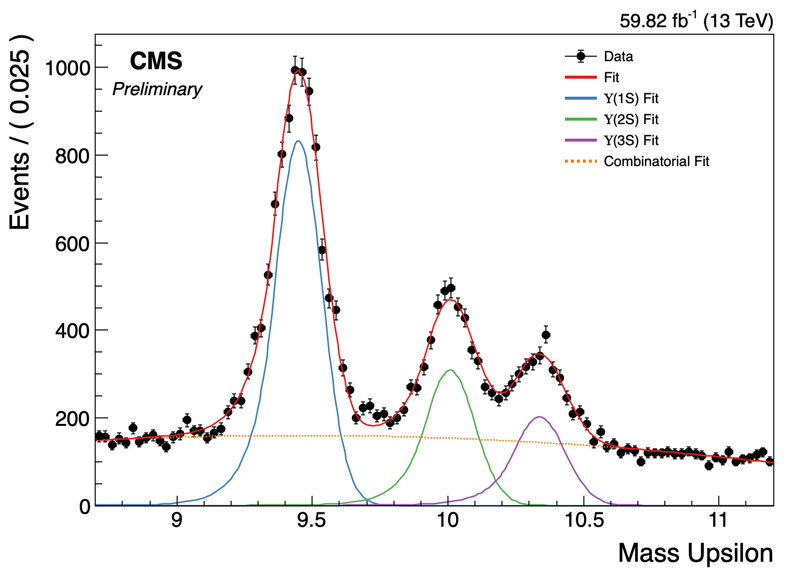
\includegraphics[width=0.68\textwidth]{figures/fit/upsilon_2018_fit.png}}
  \legend{One dimensional fit to selected $\Upsilon$ 2018 data sample. The fit is done to separate signal from the background for the three $\Upsilon$ states. The curves represent the fit for the full model (red) and each of the components (blue, green and purple for the $\Upsilon(1S)$, $\Upsilon(2S)$ and $\Upsilon(3S)$ signal and dashed orange for the combinatorial background).}
\end{figure}

\subsection{\texorpdfstring{D$^{*}$}{D*} Model}

For D$^*$ signal component, it is used a Johnson's distribution
\begin{equation}\label{eq:dstar_sig}
  S_{D^*}(\Delta m) = \frac{\delta}{\lambda\sqrt{2\pi}} \frac{1}{\sqrt{1 + \left(\frac{\Delta m-\mu}{\lambda}\right)^2}}\exp{\left[-\frac{1}{2}\left(\gamma+\delta\sinh^{-1}\left(\frac{\Delta m-\mu}{\lambda}\right)\right)^2\right]},
\end{equation}
where $\delta$, $\lambda$, $\gamma$ and $\mu$ are the free parameters. This function is often used to describe the mass difference of charm decays and fits well the $\Delta$m distribution.

For the D$^*$ background, a threshold function \cite{ZEUS:2013fws} given by:
\begin{equation} \label{eq:dstar_bkg}
  B_{D^*}(\Delta m) = A \cdot (\Delta m - m_\pi)^B \cdot \exp[C\cdot (\Delta m-m_\pi)]
\end{equation}
is used, where $m_\pi$ is the pion mass and $A$, $B$ and $C$ are free parameters.

The 1D fit to the 2018 data sample is given in Fig. \ref{fig:fit1D_dstar}.

\begin{figure}[!htm]{15cm}
  \caption{One dimensional fit to the selected D$^{*\pm}$ data}%
  \label{fig:fit1D_dstar}
  \fbox{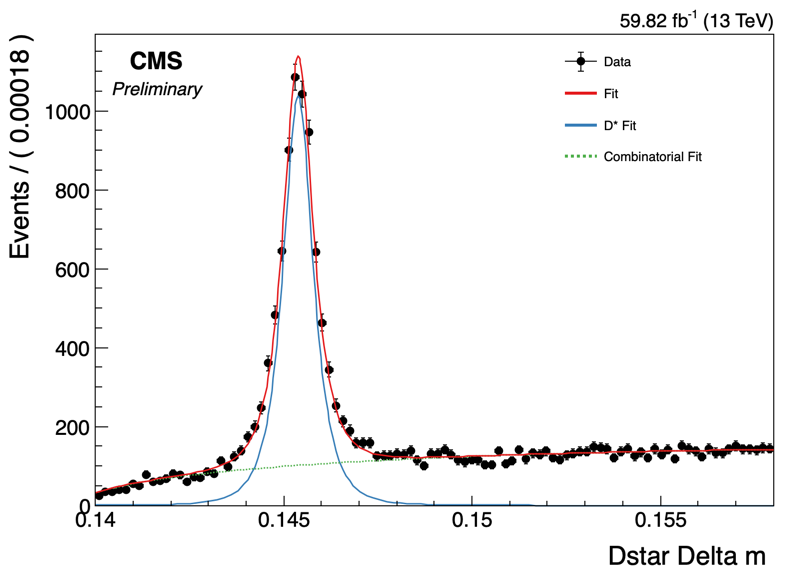
\includegraphics[width=0.68\textwidth]{figures/fit/dstar_2018_fit.png}}
  \legend{One dimensional fit to the selected D$^{*\pm}$ 2018 data sample. The curves represent the fit for the full model (red) and each of the components (blue for signal and dashed green for the combinatorial background).}
\end{figure}

\subsection{\texorpdfstring{$\Upsilon$ + D$^{*}$}{Y+D*} 2D Model}

Finally, the construction of the 2D model takes into account the 4 distributions from Eqs. \ref{eq:upsilon_sig}, \ref{eq:upsilon_bkg}, \ref{eq:dstar_sig} and \ref{eq:dstar_bkg}, creating the final four component distribution:
\begin{equation}
\begin{split}
  M_{\Upsilon D^*}(m_{\mu\mu}, \Delta m) & = f_s \cdot S_\Upsilon(m_{\mu\mu}) \cdot S_{D^*}(\Delta m) \\
  & + f_{b1} \cdot S_\Upsilon(m_{\mu\mu}) \cdot B_{D^*}(\Delta m) \\
  & + f_{b1} \cdot B_\Upsilon(m_{\mu\mu}) \cdot S_{D^*}(\Delta m) \\ 
  & + (1-f_{b1}-f_{b2}) \cdot B_\Upsilon(m_{\mu\mu}) \cdot B_{D^*}(\Delta m)
\end{split}
\end{equation}

The firs component, composed by both signal models, is used to estimate the associated $\Upsilon$ and D$^*$ yield.

The projections to the dimuon invariant mass and D$^*$ $\Delta$m, extracted from the fit for all data samples, are given in Fig. \ref{fig:fit2D_upsilondstar}.

\begin{landscape}
  \begin{figure}[!htm]{23.7cm}
    \caption{Projections of the two dimensional fit to the selected associated $\Upsilon +$ D$^{*\pm}$ for all data samples.} 
    \label{fig:fit2D_upsilondstar}
    \subfloat[][2016APV $\Upsilon$ projection.]{\label{subfig:fit2D_upsilon_proj_2016APV}%
      \fbox{\includegraphics[width=0.23\textwidth]{figures/fit/fit2D_upsilon_proj_2016APV.png}}}\hfill
    \subfloat[][2016 $\Upsilon$ projection.]{\label{subfig:fit2D_upsilon_proj_2016}%
      \fbox{\includegraphics[width=0.23\textwidth]{figures/fit/fit2D_upsilon_proj_2016.png}}}\hfill
    \subfloat[][2017 $\Upsilon$ projection.]{\label{subfig:fit2D_upsilon_proj_2017}%
      \fbox{\includegraphics[width=0.23\textwidth]{figures/fit/fit2D_upsilon_proj_2017.png}}}\hfill
    \subfloat[][2018 $\Upsilon$ projection.]{\label{subfig:fit2D_upsilon_proj_2018}%
      \fbox{\includegraphics[width=0.23\textwidth]{figures/fit/fit2D_upsilon_proj_2018.png}}}\\
    \subfloat[][2016APV D$^{*\pm}$ projection.]{\label{subfig:fit2D_dstar_proj_2016APV}%
      \fbox{\includegraphics[width=0.23\textwidth]{figures/fit/fit2D_dstar_proj_2016APV.png}}}\hfill
    \subfloat[][2016 D$^{*\pm}$ projection.]{\label{subfig:fit2D_dstar_proj_2016}%
      \fbox{\includegraphics[width=0.23\textwidth]{figures/fit/fit2D_dstar_proj_2016.png}}}\hfill
    \subfloat[][2017 D$^{*\pm}$ projection.]{\label{subfig:fit2D_dstar_proj_2017}%
      \fbox{\includegraphics[width=0.23\textwidth]{figures/fit/fit2D_dstar_proj_2017.png}}}\hfill
    \subfloat[][2018 D$^{*\pm}$ projection.]{\label{subfig:fit2D_dstar_proj_2018}%
      \fbox{\includegraphics[width=0.23\textwidth]{figures/fit/fit2D_dstar_proj_2018.png}}}\\
    \legend{Projections to the dimuon invariant mass (a-d) and D$^{*\pm}$ $\Delta$m (e-f) taken from the fit to the selected associated $\Upsilon + $ D$^{*\pm}$ for all data samples. The curves represent the full fit (in red) and each of the components - signal in blue and continuous line and background components using dashed lines in green, purple and orange.}
  \end{figure}
\end{landscape}

The summary of the fits parameters for each of the samples are found in Tabs. \ref{tab:fit_summary_2016APV} to \ref{tab:fit_summary_2018}

\begin{table}[!htbp]{15cm}
  \caption{Summary of fit parameters for the sample 2016APV}\label{tab:fit_summary_2016APV}
  \begin{tabular}{ c | c }
    Parameter & Value \\ 
    \hline
    N$_{evt}$                    & 6785 \\ \hline
    N$_{sig} \Upsilon(1S)$       & $427 \pm 51$ \\ \hline
    N$_{sig} \Upsilon(2S)$       & $165 \pm 23$ \\ \hline
    N$_{sig} \Upsilon(3S)$       & $111 \pm 17$ \\ \hline
    m$_{scale}$                  & $0.9981 \pm 0.0004$ \\ \hline
    $\Delta$m mean               & $145.35 \pm 0.04$ MeV \\ \hline
    $\chi^2 \Upsilon$ projection & 1.55 \\ \hline
    $\chi^2 D^{*\pm}$ projection & 1.64 \\ \hline
  \end{tabular}
  \legend{A summary with the more important fit parameters for sample 2016APV.}
\end{table}

\begin{table}[!htbp]{15cm}
  \caption{Summary of fit parameters for the sample 2016}\label{tab:fit_summary_2016}
  \begin{tabular}{ c | c }
    Parameter & Value \\ 
    \hline
    N$_{evt}$                    & 6421 \\ \hline
    N$_{sig} \Upsilon(1S)$       & $479 \pm 35$ \\ \hline
    N$_{sig} \Upsilon(2S)$       & $174 \pm 17$ \\ \hline
    N$_{sig} \Upsilon(3S)$       & $141 \pm 15$ \\ \hline
    m$_{scale}$                  & $0.9981 \pm 0.0004$ \\ \hline
    $\Delta$m mean               & $145.42 \pm 0.01$ MeV \\ \hline
    $\chi^2 \Upsilon$ projection & 1.19 \\ \hline
    $\chi^2 D^{*\pm}$ projection & 1.56 \\ \hline
  \end{tabular}
  \legend{A summary with the more important fit parameters for sample 2016.}
\end{table}

\begin{table}[!htbp]{15cm}
  \caption{Summary of fit parameters for the sample 2017}\label{tab:fit_summary_2017}
  \begin{tabular}{ c | c }
    Parameter & Value \\ 
    \hline
    N$_{evt}$                    & 8454 \\ \hline
    N$_{sig} \Upsilon(1S)$       & $613 \pm 53$ \\ \hline
    N$_{sig} \Upsilon(2S)$       & $230 \pm 22$ \\ \hline
    N$_{sig} \Upsilon(3S)$       & $184 \pm 18$ \\ \hline
    m$_{scale}$                  & $0.9982 \pm 0.0003$ \\ \hline
    $\Delta$m mean               & $145.37 \pm 0.04$ MeV \\ \hline
    $\chi^2 \Upsilon$ projection & 1.07 \\ \hline
    $\chi^2 D^{*\pm}$ projection & 1.15 \\ \hline
  \end{tabular}
  \legend{A summary with the more important fit parameters for sample 2017.}
\end{table}

\begin{table}[!htbp]{15cm}
  \caption{Summary of fit parameters for the sample 2018}\label{tab:fit_summary_2018}
  \begin{tabular}{ c | c }
    Parameter & Value \\ 
    \hline 
    N$_{evt}$                    & 16765 \\ \hline
    N$_{sig} \Upsilon(1S)$       & $1200 \pm 70$ \\ \hline
    N$_{sig} \Upsilon(2S)$       & $478 \pm 31$ \\ \hline
    N$_{sig} \Upsilon(3S)$       & $310 \pm 22$ \\ \hline
    m$_{scale}$                  & $0.9987 \pm 0.0002$ \\ \hline
    $\Delta$m mean               & $145.39 \pm 0.02$ MeV \\ \hline
    $\chi^2 \Upsilon$ projection & 1.28 \\ \hline
    $\chi^2 D^{*\pm}$ projection & 1.12 \\ \hline
  \end{tabular}
  \legend{A summary with the more important fit parameters for sample 2018.}
\end{table}

\section{Acceptance and Efficiency}

The acceptance and efficiency of the process is determined from the signal MC. The strategy for computing the acceptance and efficiency is to factorize it into the components,
\begin{equation}
  (Acc\cdot\epsilon) = (Acc\cdot\epsilon_{precuts})^\Upsilon \cdot 
  (Acc\cdot\epsilon_{precuts})^{D^*} \cdot \epsilon_{cuts}^\Upsilon \cdot 
  \epsilon_{cuts}^{D^*} \cdot \epsilon_{HLT} \cdot \epsilon_{association},
\end{equation}
where the $Acc\cdot\epsilon_{precuts}$ is the acceptance coupled to the precuts efficiency, $\epsilon_{cuts}$ is the selection cuts efficiency, $\epsilon_{HLT}$ is the trigger efficiency and the $\epsilon_{association}$ is the efficiency related to the $\Upsilon+D^*$ association criteria. Sec. \ref{sec:evtsel} gives details of the precuts and cuts applied.

Each of the components are calculated to create two dimensional maps used to extract the efficiency of the data samples.

\subsection{Acceptance}

The acceptance is calculated taking into account the precuts (Tab. \ref{tab:preselectioncuts}) and the cuts that define the fiducial volume of the sample on Tab. \ref{tab:fiducialvol}. The acceptance coupled to the precuts is calculated by
\begin{equation}
    (Acc \cdot \epsilon_{precuts})^P = \frac{N_{reco}^P}{N_{gen}^P},
\end{equation}
where the superscript P refers either to $\Upsilon$ or D$^*$, $N_{gen}$ is the number of generated particles within the fiducial volume, and $N_{reco}$ is the number of reconstructed particles within the same fiducial volume, passing the precuts and satisfying the respective matching criteria for that kind of particle:
\begin{itemize}
  \item For $\Upsilon$: the two muons used for its reconstruction must be matched to the muons from the decay of the generated Y within a cone of $\Delta R = \sqrt{\Delta \eta^2 + \Delta \phi^2} < 0.03$.
  \item For $D^*$: The reconstructed $D^*$ matches the generated $D^*$ with the requirements:
  $$\frac{|p_T^{reco} - p_T^{gen}|}{p_T^{gen}} < 0.2, |\eta_{gen} - \eta_{reco}|
  < 0.3, remainder(|\phi_{gen} - \phi_{reco}|, 2\pi) < 0.3.$$
\end{itemize}

The plots of the acceptance extracted from the 2018 MC sample are given in Figs. \ref{fig:acc_dimu} and \ref{fig:acc_dstar} for $\Upsilon$ and D$^*$, respectively.

\begin{figure}[!htm]{15cm}
  \caption{$\Upsilon$ acceptance of the selected associated $\Upsilon +$ D$^*$ extracted from 2018 MC sample.} 
  \label{fig:acc_dimu}
  \subfloat[][]{\label{subfig:acc_dimu_pt}%
    \fbox{\includegraphics[width=0.47\textwidth]{figures/efficiency/acc_dimu_pt_2018.png}}}\hfill
  \subfloat[][]{\label{subfig:acc_dimu_rap}%
    \fbox{\includegraphics[width=0.47\textwidth]{figures/efficiency/acc_dimu_rap_2018.png}}}\hfill\\
    \subfloat[][]{\label{subfig:acc_dimu_2D}%
    \fbox{\includegraphics[width=0.47\textwidth]{figures/efficiency/acc_dimu_2018.png}}}\\
  \legend{$\Upsilon$ acceptance extracted from the 2018 MC data sample. The acceptance is given with respect to the dimuon $p_T$ in (a), $y$ in (b), and in both $p_T$ and $y$ in (c). In (a) and (b). The horizontal dashed line is set to the upper limit of the acceptance, one.}
\end{figure}

\begin{figure}[!htm]{15cm}
  \caption{D$^*$ acceptance of the selected associated $\Upsilon +$ D$^*$ extracted from 2018 MC sample.} 
  \label{fig:acc_dstar}
  \subfloat[][]{\label{subfig:acc_dstar_pt}%
    \fbox{\includegraphics[width=0.47\textwidth]{figures/efficiency/acc_dstar_pt_2018.png}}}\hfill
  \subfloat[][]{\label{subfig:acc_dstar_rap}%
    \fbox{\includegraphics[width=0.47\textwidth]{figures/efficiency/acc_dstar_rap_2018.png}}}\hfill\\
    \subfloat[][]{\label{subfig:acc_dstar_2D}%
    \fbox{\includegraphics[width=0.47\textwidth]{figures/efficiency/acc_dstar_2018.png}}}\\
  \legend{D$^*$ acceptance extracted from the 2018 MC data sample. The acceptance is given with respect to the reconstructed D$^*$ $p_T$ in (a), $y$ in (b), and in both $p_T$ and $y$ in (c). In (a) and (b). The horizontal dashed line is set to the upper limit of the acceptance, one.}
\end{figure}

\subsection{Selection Cuts Efficiency}

The cuts considered for this efficiency component are the ones stated in the Tab. \ref{tab:selectioncuts} with exception to the cut on the $\mu\mu\pi_s$ vertex probability cut, which is treated separately. The denominator is the number of reconstructed events that passed the precuts criteria and the numerator is the number of events that passed the cuts and the precuts:
\begin{equation}
  \epsilon_{cuts}^P = \frac{N_{reco\&cuts}^P}{N_{reco}^P} (P = \Upsilon, D^*).
\end{equation}

The plots of the selection cuts efficiency extracted from the 2018 MC sample are given in Figs. \ref{fig:eff_cuts_dimu} and \ref{fig:eff_cuts_dstar} for $\Upsilon$ and D$^*$, respectively.

\begin{figure}[!htm]{15cm}
  \caption{$\Upsilon$ selection cuts efficiency of the selected associated $\Upsilon +$ D$^*$ extracted from 2018 MC sample.} 
  \label{fig:eff_cuts_dimu}
  \subfloat[][]{\label{subfig:eff_cuts_dimu_pt}%
    \fbox{\includegraphics[width=0.47\textwidth]{figures/efficiency/eff_cuts_dimu_pt_2018.png}}}\hfill
  \subfloat[][]{\label{subfig:eff_cuts_dimu_rap}%
    \fbox{\includegraphics[width=0.47\textwidth]{figures/efficiency/eff_cuts_dimu_rap_2018.png}}}\hfill\\
    \subfloat[][]{\label{subfig:eff_cuts_dimu_2D}%
    \fbox{\includegraphics[width=0.47\textwidth]{figures/efficiency/eff_cuts_dimu_2018.png}}}\\
  \legend{$\Upsilon$ selection cuts efficiency extracted from the 2018 MC data sample. This efficiency is given with respect to the dimuon $p_T$ in (a), $y$ in (b), and in both $p_T$ and $y$ in (c). In (a) and (b). The horizontal dashed line is set to the upper limit of the efficiency.}
\end{figure}

\begin{figure}[!htm]{15cm}
  \caption{D$^*$ selection cuts efficiency of the selected associated $\Upsilon +$ D$^*$ extracted from 2018 MC sample.} 
  \label{fig:eff_cuts_dstar}
  \subfloat[][]{\label{subfig:eff_cuts_dstar_pt}%
    \fbox{\includegraphics[width=0.47\textwidth]{figures/efficiency/eff_cuts_dstar_pt_2018.png}}}\hfill
  \subfloat[][]{\label{subfig:eff_cuts_dstar_rap}%
    \fbox{\includegraphics[width=0.47\textwidth]{figures/efficiency/eff_cuts_dstar_rap_2018.png}}}\hfill\\
    \subfloat[][]{\label{subfig:eff_cuts_dstar_2D}%
    \fbox{\includegraphics[width=0.47\textwidth]{figures/efficiency/eff_cuts_dstar_2018.png}}}\\
  \legend{D$^*$ selection cuts efficiency extracted from the 2018 MC data sample. This efficiency is given with respect to the D$^*$ $p_T$ in (a), $y$ in (b), and in both $p_T$ and $y$ in (c). In (a) and (b). The horizontal dashed line is set to the upper limit of the efficiency.}
\end{figure}

\subsection{Trigger Efficiency}

The triggers used depend only on the dimuons, therefore, their efficiency is only evaluated from the $\Upsilon$ candidates. The denominator is the number of events that passed both the precuts and cuts criteria and the numerator the number of events passing the trigger, cuts and precuts:
\begin{equation}
  \epsilon_{HLT} = \frac{N_{reco\&cuts\&trigger}^\Upsilon}{N_{reco\&cuts}^\Upsilon}
\end{equation}

The plots of the trigger efficiency extracted from the 2018 MC sample are given in Fig. \ref{fig:eff_trigger}.

\begin{figure}[!htm]{15cm}
  \caption{Trigger efficiency of the selected associated $\Upsilon +$ D$^*$ extracted from 2018 MC sample.} 
  \label{fig:eff_trigger}
  \subfloat[][]{\label{subfig:eff_trigger_pt}%
    \fbox{\includegraphics[width=0.47\textwidth]{figures/efficiency/eff_trigger_pt_2018.png}}}\hfill
  \subfloat[][]{\label{subfig:eff_trigger_rap}%
    \fbox{\includegraphics[width=0.47\textwidth]{figures/efficiency/eff_trigger_rap_2018.png}}}\hfill\\
    \subfloat[][]{\label{subfig:eff_trigger_2D}%
    \fbox{\includegraphics[width=0.47\textwidth]{figures/efficiency/eff_trigger_2018.png}}}\\
  \legend{Trigger efficiency extracted from the 2018 MC data sample. This efficiency is given with respect to the dimuon $p_T$ in (a), $y$ in (b), and in both $p_T$ and $y$ in (c). In (a) and (b). The horizontal dashed line is set to the upper limit of the efficiency.}
\end{figure}

\subsection{Association efficiency}

The last efficiency is related to the association between $\Upsilon$ and $D^*$. It is given by
\begin{equation}
  \epsilon_{association} = 
  \frac{N_{reco\&cuts\&trigger\&association}^{\Upsilon D^*}}{N_{reco\&cuts\&trigger}^{\Upsilon D^*}},
\end{equation}
where the denominator is the number events that passed all the previous selections and the numerator is the number of events after the addition of the association cut, which is the $\mu\mu\pi_s$ vertex probability $> 0.01$.

The plots of the trigger efficiency extracted from the 2018 MC sample are given in Fig. \ref{fig:eff_asso}.

\begin{figure}[!htm]{15cm}
  \caption{Trigger efficiency of the selected associated $\Upsilon +$ D$^*$ extracted from 2018 MC sample.} 
  \label{fig:eff_asso}
  \subfloat[][]{\label{subfig:eff_asso_pt}%
    \fbox{\includegraphics[width=0.47\textwidth]{figures/efficiency/eff_asso_pt_2018.png}}}\hfill
  \subfloat[][]{\label{subfig:eff_asso_rap}%
    \fbox{\includegraphics[width=0.47\textwidth]{figures/efficiency/eff_asso_rap_2018.png}}}\hfill\\
  \legend{Associuation efficiency extracted from the 2018 MC data sample. The efficiency maps are given with respect to the dimuon and D$^*$ $p_T$ in (a) and $y$ in (b).}
\end{figure}

\subsection{Total efficiency}\label{sec:total_eff}

The shown efficiency maps are used to calculate efficiency that will be used in the cross section determination. The final efficiency for each subsample is shown in Tab. \ref{tab:totaleff}.

\begin{table}[!htbp]{15cm}
  \caption{Total efficiency per data sample.}
  \begin{tabular}{ l | c }
    \hline
    \multicolumn{1}{c|}{Sample} & \multicolumn{1}{c}{Total Efficiency (\%)} \\ \hline
    2016APV & $7.5^{+1.0}_{-1.6}$ \\ \hline
    2016    & $9.3^{+1.1}_{-2.6}$ \\ \hline
    2017    & $6.9^{+1.2}_{-1.7}$ \\ \hline
    2018    & $4.4^{+1.5}_{-1.7}$ \\ \hline
  \end{tabular}
  \legend{Total efficiency per data sample. The uncertainties shown are only statistical.}
  \label{tab:totaleff}
\end{table}

It is worth noting that the efficiencies displayed here are measured using a private MC with reduced statistics, resulting in a bigger uncertainties, in special for the sample 2018, with uncertainty of $\approx$ 30 \%. A new generation, with higher statistics is being processed, so it is expected that the efficiency will be better determined in the future.

\section{Associated \texorpdfstring{$\Upsilon(nS)$ + D$^{*}$}{Y+D*} Cross Section}

\subsection{Fiducial Cross Section} \label{subsec:fiducial_xsec}

The cross section of the associated $\Upsilon$ + D$^{*}$ is calculated by the formula:
\begin{equation}
  \sigma_{\Upsilon(nS) D^*} = \frac{N_{\Upsilon(nS) D^*}}{L\cdot eff \cdot BR(\Upsilon(nS))BR(D^*)},
\end{equation}
where $nS$ refers to the $\Upsilon$ states (1S, 2S and 3S), $N_{\Upsilon(nS) D^*}$ is the number of associated $\Upsilon(nS)$ + D$^*$ extracted from the 2D fit, $L$ is the integrated luminosity of the sample (Sec. \ref{sec:trigger}), $eff$ is the total efficiency (Sec. \ref{sec:total_eff}) and $BR(\Upsilon(nS))$ and $BR(D^*)$ are the branch ratios of $\Upsilon$ and D$^*$, respectively.

Table \ref{tab:DPS_xsec} presents the fiducial cross section for each data sample and $\Upsilon$ state. The values are compatible with each other so that the can be combined.

\begin{table}[!htbp]{15cm}
  \caption{$\Upsilon(nS)$ + D$^{*}$ fiducial cross section per data sample.}
  \begin{tabular}{ l | l | c }
    \hline
    Associated measurement & Sample & Cross section (pb) \\ \hline
    \multirow[c]{4}{*}{$\Upsilon(1S)$ + D$^{*\pm}$} 
    & 2016APV & $444^{+77}_{-107}$ \bigstrut\\\cline{2-3} 
    & 2016    & $462^{+66}_{-134}$ \bigstrut\\\cline{2-3} 
    & 2017    & $495^{+96}_{-128}$ \bigstrut\\\cline{2-3} 
    & 2018    & $680^{+237}_{-266}$ \\ \hline
    \multirow[c]{4}{*}{$\Upsilon(2S)$ + D$^{*\pm}$} 
    & 2016APV & $221^{+41}_{-55}$ \bigstrut\\\cline{2-3} 
    & 2016    & $216^{+34}_{-64}$ \bigstrut\\\cline{2-3} 
    & 2017    & $239^{+47}_{-62}$ \bigstrut\\\cline{2-3} 
    & 2018    & $349^{+122}_{-137}$ \\ \hline
    \multirow[c]{4}{*}{$\Upsilon(3S)$ + D$^{*\pm}$} 
    & 2016APV & $131^{+26}_{-34}$ \bigstrut\\\cline{2-3} 
    & 2016    & $155^{+25}_{-47}$ \bigstrut\\\cline{2-3} 
    & 2017    & $169^{+34}_{-44}$ \bigstrut\\\cline{2-3} 
    & 2018    & $200^{+70}_{-79}$ \\ \hline
  \end{tabular}
  \legend{$\Upsilon(nS)$ + D$^{*}$ cross section per data sample. The cross section is determined for each of the $\Upsilon$ states and its uncertainties are only statistical.}
  \label{tab:DPS_xsec}
\end{table}

Finally, the combined cross section for each $\Upsilon$ state are:
\begin{equation}
\begin{split}
  \sigma_{Y(1S)D^{*\pm}} &= 474^{+44}_{-68} \; \text{pb},\\
  \sigma_{Y(2S)D^{*\pm}} &= 230^{+23}_{-34} \; \text{pb},\\
  \sigma_{Y(3S)D^{*\pm}} &= 152^{+16}_{-22} \; \text{pb},
\end{split} 
\end{equation}
where only statistical errors are considered.

\subsection{Effective Cross Section}

The effective cross section can be determined by rearranging the Eq. \ref{eq:xsecDPS}
\begin{equation}
  \sigma_{eff} = \frac{\sigma_\Upsilon \cdot \sigma_{D^*}}{\sigma_{\Upsilon D^*}^{DPS}}.
\end{equation}
The $\sigma^{DPS}$ is different from the cross section determined in Sec. \ref{subsec:fiducial_xsec}, as this one is composed from the SPS and DPS components. It is possible to write
\begin{equation}
  \sigma_{\Upsilon D^*} = \sigma_{\Upsilon D^*}^{SPS} + \sigma_{\Upsilon D^*}^{DPS}.
\end{equation}
To calculate the $\sigma_{eff}$, the fraction of the DPS contribution needs to be computed, which is normally done by inspection of the $\Delta$y and/or $\Delta\phi$ distributions \cite{Lansberg:2019adr}. In this work, the fraction is assumed to be one, and the value presented can be assumed as a lower bound for the $\sigma_{eff}$.

The inclusive cross section of $\Upsilon(nS)$ and D$^*$ can be found in Tab. \ref{tab:inclusive_xsec}.

\begin{table}[!htbp]{15cm}
  \caption{Fiducial cross section of $\Upsilon(nS)$ and D$^*$.}
  \begin{tabular}{ c | c | c }
    \hline
    Particle & Fiducial cross section & Kinematic region \\ \hline
    $\Upsilon(1S)$ & $87.7 \pm 1.4 \text{(stat)} \pm 5.3 \text{(syst)}$ pb  & \multirow[c]{3}{*}{$20 < p_T < 130$ GeV, $|y| < 1.2$} \bigstrut\\\cline{1-2}  
    $\Upsilon(2S)$ & $39.4 \pm 1.0 \text{(stat)} \pm 2.4 \text{(syst)}$ pb  &  \bigstrut\\\cline{1-2} 
    $\Upsilon(3S)$ & $28.2 \pm 0.9 \text{(stat)} \pm 1.9 \text{(syst)}$ pb  & \bigstrut\\\cline{1-3} 
    $D^*$          & $380 \pm 17 \text{(stat)} \pm 46 \text{(syst)}$ $\mu$b & $4 < p_T < 100$ GeV, $|\eta| < 2.1$ \\ \hline
  \end{tabular}
  \legend{Fiducial cross section of $\Upsilon(nS)$ and D$^*$ derived from the differencial cross section from the sources.}
  \label{tab:inclusive_xsec}
  \source{\cite{CMS:2017dju, CMS:2021lab}}
\end{table}

Since the kinematic region in Tab. \ref{tab:inclusive_xsec} are different from the ones chosen in the cross section determination in Sec. \ref{subsec:fiducial_xsec} these numbers cannot be used directly in the $\sigma_{eff}$ calculation. One simple way to solve this problem is to restrict the associated $\Upsilon$ + D$^*$ fiducial cross section to match the phase space of the inclusive measurement. This restriction have the effect of lowering the number of events of the samples, which is bad for the fit procedure, in special for the $\Upsilon(2S)$ and $\Upsilon(3S)$ in the 2016 and 2016APV subsamples, which have less statistics as shown in Fig. \ref{fig:fit2D_upsilondstar_rest}. For this reason, the lower limit for effective cross section will be determined only for $\Upsilon(1S) +$ D$^*$. Table \ref{tab:xsec_eff} displays a summary the values for the $\sigma_{eff}$ lower bound, as well as other important parameters.

\begin{table}[!htbp]{15cm}
  \caption{Lower bound for $\Upsilon(1S)$ + D$^{*}$ effective cross section per data sample.}
  \begin{tabular}{ c | c | c | c | c }
    \hline
    Sample & eff (\%) & N & $\sigma$ (pb) & $\sigma_{eff}$ (mb) \\ \hline
    2016APV & $8.4^{+1.0}_{-1.5}$ & $147 \pm 33$ & $136^{+35}_{-40}$ & $>9.9^{+2.6}_{-2.9}$ \\ \hline 
    2016    & $10.5^{+1.1}_{-2.6}$ & $190 \pm 42$ & $162^{+40}_{-54}$ & $>8.3^{+2.1}_{-2.8}$ \\ \hline 
    2017    & $8.2^{+1.2}_{-1.7}$ & $250 \pm 34$ & $170^{+33}_{-42}$ & $>7.9^{+1.6}_{-2.0}$ \\ \hline 
    2018    & $6.0^{+1.4}_{-1.6}$ & $479 \pm 51$ & $203^{+51}_{-59}$ & $>6.6^{+1.7}_{-2.0}$ \\ \hline
  \end{tabular}
  \legend{Lower bound for $\Upsilon(1S)$ + D$^{*}$ effective cross section per data sample. For the lower bound determination, the fraction of DPS is assumed to be one. All the uncertainties displayed are only statistical.}
  \label{tab:xsec_eff}
\end{table}

Finally, combining all the values from Tab. \ref{tab:xsec_eff}, it is possible to determine the limit for the sigma effective:
\begin{equation}
  \sigma_{eff} > 8.1^{+1.0}_{-1.2} \; \text{mb}.
\end{equation}

\begin{landscape}
  \begin{figure}[!htm]{23.7cm}
    \caption{Projections of the two dimensional fit to the selected associated $\Upsilon +$ D$^{*\pm}$ on the restricted phase space sample.} 
    \label{fig:fit2D_upsilondstar_rest}
    \subfloat[][2016APV $\Upsilon$ projection.]{\label{subfig:fit2D_rest_upsilon_proj_2016APV}%
      \fbox{\includegraphics[width=0.23\textwidth]{figures/fit_rest/fit2D_upsilon_proj_2016APV.png}}}\hfill
    \subfloat[][2016 $\Upsilon$ projection.]{\label{subfig:fit2D_rest_upsilon_proj_2016}%
      \fbox{\includegraphics[width=0.23\textwidth]{figures/fit_rest/fit2D_upsilon_proj_2016.png}}}\hfill
    \subfloat[][2017 $\Upsilon$ projection.]{\label{subfig:fit2D_rest_upsilon_proj_2017}%
      \fbox{\includegraphics[width=0.23\textwidth]{figures/fit_rest/fit2D_upsilon_proj_2017.png}}}\hfill
    \subfloat[][2018 $\Upsilon$ projection.]{\label{subfig:fit2D_rest_upsilon_proj_2018}%
      \fbox{\includegraphics[width=0.23\textwidth]{figures/fit_rest/fit2D_upsilon_proj_2018.png}}}\\
    \subfloat[][2016APV D$^{*\pm}$ projection.]{\label{subfig:fit2D_rest_dstar_proj_2016APV}%
      \fbox{\includegraphics[width=0.23\textwidth]{figures/fit_rest/fit2D_dstar_proj_2016APV.png}}}\hfill
    \subfloat[][2016 D$^{*\pm}$ projection.]{\label{subfig:fit2D_rest_dstar_proj_2016}%
      \fbox{\includegraphics[width=0.23\textwidth]{figures/fit_rest/fit2D_dstar_proj_2016.png}}}\hfill
    \subfloat[][2017 D$^{*\pm}$ projection.]{\label{subfig:fit2D_rest_dstar_proj_2017}%
      \fbox{\includegraphics[width=0.23\textwidth]{figures/fit_rest/fit2D_dstar_proj_2017.png}}}\hfill
    \subfloat[][2018 D$^{*\pm}$ projection.]{\label{subfig:fit2D_rest_dstar_proj_2018}%
      \fbox{\includegraphics[width=0.23\textwidth]{figures/fit_rest/fit2D_dstar_proj_2018.png}}}\\
    \legend{Projections to the dimuon invariant mass (a-d) and D$^{*\pm}$ $\Delta$m (e-f) taken from the fit to the selected associated $\Upsilon + $ D$^{*\pm}$ for all data samples restricting the phase space to match the ones specified in Tab. \ref{tab:inclusive_xsec}. The curves represent the full fit (in red) and each of the components - signal in blue and continuous line and background components using dashed lines in green, purple and orange.}
  \end{figure}
\end{landscape}

\section{Systematic Uncertainties}

The systematic uncertainties include all the uncertainties that do not arise from the fluctuations in a finite set of measurements. This includes bias coming from the experiment, the assumptions made and models used to make the conclusions. The evaluation of this kind of uncertainty is analysis dependant, as one needs to consider all assumptions made in the measurement process.

That being said, the complete systematic uncertainty definition is not finished in this analysis due to time constraints, but some of them are brought in the following lines.

\begin{itemize}
  \item \textbf{Integrated Luminosity}: The integrated luminosity uncertainties are given in Refs. \cite{CMS-PAS-LUM-17-001, CMS-PAS-LUM-17-004, CMS-PAS-LUM-18-002} and are summarized in Tab. \ref{tab:triggers}. 
  \item \textbf{Branching Fraction}: The uncertainties on the branching fractions of each considered decay channel are given in Ref. \cite{Workman:2022ynf}. The values are pointed out in Sec. \ref{sec:theoryY+D}
  \item \textbf{Determination of the yields}: This systematic depends on the models used to determine the signal and background yields, in general, the models used to describe the shapes of the distributions. For D$^*$ signal, the model was changed to a double Gaussian and for the background another threshold function was used \cite{CMS:2021lab}, with the form
  \begin{equation}
    f = \left[ 1- \exp{\left( -\frac{\Delta m - m_\pi}{p_0} \right)} \right]\left( \frac{\Delta m}{m_\pi} \right)^{p_1} +p_2 \left( \frac
    {\Delta m}{m_\pi} - 1 \right),
  \end{equation}
  where $m_\pi$ is taken as the pion mass and $p_0$, $p_1$ and $p_2$ are free parameters. The deviations from the yields were taken as systematic uncertainties.

  For $\Upsilon$ signal, a change from CBs to Gaussians resulted to bad fits, as the later one cannot describe well the tails of the invariant mass distribution. Another method is to evaluate the CB shape changes with the change of its parameters. The tail parameters $n$ and $\alpha$ are specially sensitive as they are strongly correlated. $n$ was left as free parameter and $\alpha$ was moved by $\pm 2\sigma$. Half of the maximum observed variation was taken as systematic, because these variations are correlated. Another parameter analyzed was the mean of the CBs, which is defined from a common factor and the mass of the $\Upsilon$ state taken from Ref. \cite{Workman:2022ynf}. The means were left as a free parameter and the deviation in the yield is taken as a systematic.

  Finally, the $\Upsilon$ background model was modified to a 3rd order Chebychev polynomials and the deviation was taken as systematic.
  \item \textbf{Selection Cuts}: The selection cuts 
  \item \textbf{Tracking Efficiencies}: The tracking efficiency for charged hadrons is given by Ref. \cite{CMS-DP-2022-012}, using the branching ratios two D$^*$ decays: $D^* \rightarrow K\pi\pi_s$ and $D^* \rightarrow K3\pi\pi_s$. The uncertainty is given depending on the sample and it is combined for the two D$^0$ tracks. For $\pi_s$, a different procedure should be done, since it has a soft $p_T$ distribution. The value of 5.2 \%, given in Ref. \cite{CMS:2021lab} is used.
\end{itemize}
%================================================================
\chapter{Conclusion and perspectives}\label{chap:conclusion}
%================================================================

The associated production of $\Upsilon(nS) + $ D$^{*\pm}$ analysis has been presented. The aim was to provide a cross section measurement of the associated production and to determine the $\sigma_{eff}$ using data from pp collisions from LHC at $\sqrt{s} = 13$ TeV, recorded by CMS during Run 2 between 2015 and 2018. The total integrated luminosity of the data samples amounts to 123 fb$^{-1}$.

The measured fiducial cross sections for each of the $\Upsilon$ states, in the fiducial region defined by the Table \ref{tab:fiducialvol}, are
\begin{equation}
  \begin{split}
    \sigma_{Y(1S)D^{*\pm}} &= 478 \pm 68 \text{(stat)} \pm 46 \text{(syst)} \; \text{pb},\\
    \sigma_{Y(2S)D^{*\pm}} &= 233 \pm 34 \text{(stat)} \pm 31 \text{(syst)} \; \text{pb},\\
    \sigma_{Y(3S)D^{*\pm}} &= 152 \pm 22 \text{(stat)} \pm 31 \text{(syst)} \; \text{pb}.
  \end{split}
\end{equation}
It is worth noting that there are further developments needed, mainly in the efficiencies calculations, which was done from a MC with restricted statistics, and a more deep determination of the systematic uncertainties.

For the effective cross section, the fiducial region had to be restricted to the one from previous measurements of $\Upsilon(nS)$ and D$^{*\pm}$ cross sections. This resulted in a bad agreement between the numbers from the $\Upsilon(2S)$ and $\Upsilon(3S)$. For this reason, this number was calculated only for $\Upsilon(1S)$, which showed good agreement between the samples. By assuming associated production is free from SPS contribution, the minimum value for the effective cross section is
\begin{equation}
  \sigma_{eff} > 7.9 \pm 1.2 \text{(stat)} \; \text{mb}.
\end{equation}
In this measurement, a way to improve the result was pointed out in Sec. \ref{sec:discussion}, which has the advantage to use the full kinematical region proposed by this analysis and to have lower systematic uncertainties sources. Also, a new MC, with higher statistics is being processed, so the efficiencies will be better determined.

Regarding the CMS RPC project, it has been presented the contributions given in the maintenance, operation and R\&D. There are many challenges for these detectors, as they have to keep the excellent timing, stability and robustness, even in the high radiation environment of the HL-LHC. Finally, because of the regulations imposed to the high GWP gases, the search of a low GWP gases to substitute freon and SF$_6$ are of most importance for the future of this gaseous detector technology.

%\index{Introdução!Capítulo}.

%XXXXXXXXXXXXXXXXXXXXXXXXXXXXXXXXXXXXXXXXXXXXXXXXXXXXXXXXXXXXXXXX
% ELEMENTOS POS-TEXTUAIS
%XXXXXXXXXXXXXXXXXXXXXXXXXXXXXXXXXXXXXXXXXXXXXXXXXXXXXXXXXXXXXXXX
\backmatter % inicia a área dos elementos pós-textuais
%XXXXXXXXXXXXXXXXXXXXXXXXXXXXXXXXXXXXXXXXXXXXXXXXXXXXXXXXXXXXXXXX

%===========================================================
% Referencias via BibTeX
%===========================================================

\citeoption{abnt-options4}
\bibliography{abnt-options4,bibliografia}

%===========================================================
\postextualchapter*{Glossário} % elemento opcional
%===========================================================

\definicao{termo 1}{significado}
\definicao{termo 2}{significado}
\definicao{termo 3}{significado}

%XXXXXXXXXXXXXXXXXXXXXXXXXXXXXXXXXXXXXXXXXXXXXXXXXXXXXXXXXXX
% Apêndices (opcionais)
%XXXXXXXXXXXXXXXXXXXXXXXXXXXXXXXXXXXXXXXXXXXXXXXXXXXXXXXXXXX
\appendix % inicia os apêndices
%XXXXXXXXXXXXXXXXXXXXXXXXXXXXXXXXXXXXXXXXXXXXXXXXXXXXXXXXXXX
%===========================================================
\postextualchapter{Efficiency maps}\label{app:efficiencies}
%===========================================================

All the Efficiency maps are used for the efficiency calculation, as explained in Sec. \ref{sec:efficiency}, are displayed here.

\section{Efficiencies for sample 2016APV}

\begin{figure}[H]{15cm}
  \caption{$\Upsilon$ acceptance of the selected associated $\Upsilon +$ D$^*$ extracted from 2016APV MC sample.}
  \label{fig:acc_dimu_2016APV}
  \subfloat[][]{\label{subfig:acc_dimu_pt_2016APV}%
    \fbox{\includegraphics[width=0.44\textwidth]{figures/efficiency/acc_dimu_pt_2016APV.png}}}\hfill
  \subfloat[][]{\label{subfig:acc_dimu_rap_2016APV}%
    \fbox{\includegraphics[width=0.44\textwidth]{figures/efficiency/acc_dimu_rap_2016APV.png}}}\hfill\\
  \subfloat[][]{\label{subfig:acc_dimu_2D_2016APV}%
    \fbox{\includegraphics[width=0.44\textwidth]{figures/efficiency/acc_dimu_2016APV.png}}}\\
  \legend{$\Upsilon$ acceptance extracted from the 2016APV MC data sample. The acceptance is given with respect to the dimuon $p_T$ in (a), $y$ in (b), and in both $p_T$ and $y$ in (c). In (a) and (b). The horizontal dashed line is set to the upper limit of the acceptance, one.}
\end{figure}

\begin{figure}[H]{15cm}
  \caption{D$^*$ acceptance of the selected associated $\Upsilon +$ D$^*$ extracted from 2016APV MC sample.}
  \label{fig:acc_dstar_2016APV}
  \subfloat[][]{\label{subfig:acc_dstar_pt_2016APV}%
    \fbox{\includegraphics[width=0.44\textwidth]{figures/efficiency/acc_dstar_pt_2016APV.png}}}\hfill
  \subfloat[][]{\label{subfig:acc_dstar_rap_2016APV}%
    \fbox{\includegraphics[width=0.44\textwidth]{figures/efficiency/acc_dstar_rap_2016APV.png}}}\hfill\\
  \subfloat[][]{\label{subfig:acc_dstar_2D_2016APV}%
    \fbox{\includegraphics[width=0.44\textwidth]{figures/efficiency/acc_dstar_2016APV.png}}}\\
  \legend{D$^*$ acceptance extracted from the 2016APV MC data sample. The acceptance is given with respect to the reconstructed D$^*$ $p_T$ in (a), $y$ in (b), and in both $p_T$ and $y$ in (c). In (a) and (b). The horizontal dashed line is set to the upper limit of the acceptance, one.}
\end{figure}

\begin{figure}[H]{15cm}
  \caption{$\Upsilon$ selection cuts efficiency of the selected associated $\Upsilon +$ D$^*$ extracted from 2016APV MC sample.}
  \label{fig:eff_cuts_dimu_2016APV}
  \subfloat[][]{\label{subfig:eff_cuts_dimu_pt_2016APV}%
  \fbox{\includegraphics[width=0.44\textwidth]{figures/efficiency/eff_cuts_dimu_pt_2016APV.png}}}\hfill
  \subfloat[][]{\label{subfig:eff_cuts_dimu_rap_2016APV}%
  \fbox{\includegraphics[width=0.44\textwidth]{figures/efficiency/eff_cuts_dimu_rap_2016APV.png}}}\hfill\\
  \subfloat[][]{\label{subfig:eff_cuts_dimu_2D_2016APV}%
  \fbox{\includegraphics[width=0.44\textwidth]{figures/efficiency/eff_cuts_dimu_2016APV.png}}}\\
  \legend{$\Upsilon$ selection cuts efficiency extracted from the 2016APV MC data sample. This efficiency is given with respect to the dimuon $p_T$ in (a), $y$ in (b), and in both $p_T$ and $y$ in (c). In (a) and (b). The horizontal dashed line is set to the upper limit of the efficiency.}
\end{figure}

\begin{figure}[H]{15cm}
  \caption{D$^*$ selection cuts efficiency of the selected associated $\Upsilon +$ D$^*$ extracted from 2016APV MC sample.}
  \label{fig:eff_cuts_dstar_2016APV}
  \subfloat[][]{\label{subfig:eff_cuts_dstar_pt_2016APV}%
    \fbox{\includegraphics[width=0.44\textwidth]{figures/efficiency/eff_cuts_dstar_pt_2016APV.png}}}\hfill
  \subfloat[][]{\label{subfig:eff_cuts_dstar_rap_2016APV}%
    \fbox{\includegraphics[width=0.44\textwidth]{figures/efficiency/eff_cuts_dstar_rap_2016APV.png}}}\hfill\\
  \subfloat[][]{\label{subfig:eff_cuts_dstar_2D_2016APV}%
    \fbox{\includegraphics[width=0.44\textwidth]{figures/efficiency/eff_cuts_dstar_2016APV.png}}}\\
  \legend{D$^*$ selection cuts efficiency extracted from the 2016APV MC data sample. This efficiency is given with respect to the D$^*$ $p_T$ in (a), $y$ in (b), and in both $p_T$ and $y$ in (c). In (a) and (b). The horizontal dashed line is set to the upper limit of the efficiency.}
\end{figure}

\begin{figure}[H]{15cm}
  \caption{Trigger efficiency of the selected associated $\Upsilon +$ D$^*$ extracted from 2016APV MC sample.}
  \label{fig:eff_trigger_2016APV}
  \subfloat[][]{\label{subfig:eff_trigger_pt_2016APV}%
    \fbox{\includegraphics[width=0.44\textwidth]{figures/efficiency/eff_trigger_pt_2016APV.png}}}\hfill
  \subfloat[][]{\label{subfig:eff_trigger_rap_2016APV}%
    \fbox{\includegraphics[width=0.44\textwidth]{figures/efficiency/eff_trigger_rap_2016APV.png}}}\hfill\\
  \subfloat[][]{\label{subfig:eff_trigger_2D_2016APV}%
    \fbox{\includegraphics[width=0.44\textwidth]{figures/efficiency/eff_trigger_2016APV.png}}}\\
  \legend{Trigger efficiency extracted from the 2016APV MC data sample. This efficiency is given with respect to the dimuon $p_T$ in (a), $y$ in (b), and in both $p_T$ and $y$ in (c). In (a) and (b). The horizontal dashed line is set to the upper limit of the efficiency.}
\end{figure}

\begin{figure}[H]{15cm}
  \caption{Trigger efficiency of the selected associated $\Upsilon +$ D$^*$ extracted from 2016APV MC sample.}
  \label{fig:eff_asso_2016APV}
  \subfloat[][]{\label{subfig:eff_asso_pt_2016APV}%
    \fbox{\includegraphics[width=0.44\textwidth]{figures/efficiency/eff_asso_pt_2016APV.png}}}\hfill
  \subfloat[][]{\label{subfig:eff_asso_rap_2016APV}%
    \fbox{\includegraphics[width=0.44\textwidth]{figures/efficiency/eff_asso_rap_2016APV.png}}}\hfill\\
  \legend{Association efficiency extracted from the 2016APV MC data sample. The efficiency maps are given with respect to the dimuon and D$^*$ $p_T$ in (a) and $y$ in (b).}
\end{figure}

\clearpage

\section{Efficiencies for sample 2016}

\begin{figure}[H]{15cm}
  \caption{$\Upsilon$ acceptance of the selected associated $\Upsilon +$ D$^*$ extracted from 2016 MC sample.}
  \label{fig:acc_dimu_2016}
  \subfloat[][]{\label{subfig:acc_dimu_pt_2016}%
    \fbox{\includegraphics[width=0.44\textwidth]{figures/efficiency/acc_dimu_pt_2016.png}}}\hfill
  \subfloat[][]{\label{subfig:acc_dimu_rap_2016}%
    \fbox{\includegraphics[width=0.44\textwidth]{figures/efficiency/acc_dimu_rap_2016.png}}}\hfill\\
  \subfloat[][]{\label{subfig:acc_dimu_2D_2016}%
    \fbox{\includegraphics[width=0.44\textwidth]{figures/efficiency/acc_dimu_2016.png}}}\\
  \legend{$\Upsilon$ acceptance extracted from the 2016 MC data sample. The acceptance is given with respect to the dimuon $p_T$ in (a), $y$ in (b), and in both $p_T$ and $y$ in (c). In (a) and (b). The horizontal dashed line is set to the upper limit of the acceptance, one.}
\end{figure}

\begin{figure}[H]{15cm}
  \caption{D$^*$ acceptance of the selected associated $\Upsilon +$ D$^*$ extracted from 2016 MC sample.}
  \label{fig:acc_dstar_2016}
  \subfloat[][]{\label{subfig:acc_dstar_pt_2016}%
    \fbox{\includegraphics[width=0.44\textwidth]{figures/efficiency/acc_dstar_pt_2016.png}}}\hfill
  \subfloat[][]{\label{subfig:acc_dstar_rap_2016}%
    \fbox{\includegraphics[width=0.44\textwidth]{figures/efficiency/acc_dstar_rap_2016.png}}}\hfill\\
  \subfloat[][]{\label{subfig:acc_dstar_2D_2016}%
    \fbox{\includegraphics[width=0.44\textwidth]{figures/efficiency/acc_dstar_2016.png}}}\\
  \legend{D$^*$ acceptance extracted from the 2016 MC data sample. The acceptance is given with respect to the reconstructed D$^*$ $p_T$ in (a), $y$ in (b), and in both $p_T$ and $y$ in (c). In (a) and (b). The horizontal dashed line is set to the upper limit of the acceptance, one.}
\end{figure}

\begin{figure}[H]{15cm}
  \caption{$\Upsilon$ selection cuts efficiency of the selected associated $\Upsilon +$ D$^*$ extracted from 2016 MC sample.}
  \label{fig:eff_cuts_dimu_2016}
  \subfloat[][]{\label{subfig:eff_cuts_dimu_pt_2016}%
  \fbox{\includegraphics[width=0.44\textwidth]{figures/efficiency/eff_cuts_dimu_pt_2016.png}}}\hfill
  \subfloat[][]{\label{subfig:eff_cuts_dimu_rap_2016}%
  \fbox{\includegraphics[width=0.44\textwidth]{figures/efficiency/eff_cuts_dimu_rap_2016.png}}}\hfill\\
  \subfloat[][]{\label{subfig:eff_cuts_dimu_2D_2016}%
  \fbox{\includegraphics[width=0.44\textwidth]{figures/efficiency/eff_cuts_dimu_2016.png}}}\\
  \legend{$\Upsilon$ selection cuts efficiency extracted from the 2016 MC data sample. This efficiency is given with respect to the dimuon $p_T$ in (a), $y$ in (b), and in both $p_T$ and $y$ in (c). In (a) and (b). The horizontal dashed line is set to the upper limit of the efficiency.}
\end{figure}

\begin{figure}[H]{15cm}
  \caption{D$^*$ selection cuts efficiency of the selected associated $\Upsilon +$ D$^*$ extracted from 2016 MC sample.}
  \label{fig:eff_cuts_dstar_2016}
  \subfloat[][]{\label{subfig:eff_cuts_dstar_pt_2016}%
    \fbox{\includegraphics[width=0.44\textwidth]{figures/efficiency/eff_cuts_dstar_pt_2016.png}}}\hfill
  \subfloat[][]{\label{subfig:eff_cuts_dstar_rap_2016}%
    \fbox{\includegraphics[width=0.44\textwidth]{figures/efficiency/eff_cuts_dstar_rap_2016.png}}}\hfill\\
  \subfloat[][]{\label{subfig:eff_cuts_dstar_2D_2016}%
    \fbox{\includegraphics[width=0.44\textwidth]{figures/efficiency/eff_cuts_dstar_2016.png}}}\\
  \legend{D$^*$ selection cuts efficiency extracted from the 2016 MC data sample. This efficiency is given with respect to the D$^*$ $p_T$ in (a), $y$ in (b), and in both $p_T$ and $y$ in (c). In (a) and (b). The horizontal dashed line is set to the upper limit of the efficiency.}
\end{figure}

\begin{figure}[H]{15cm}
  \caption{Trigger efficiency of the selected associated $\Upsilon +$ D$^*$ extracted from 2016 MC sample.}
  \label{fig:eff_trigger_2016}
  \subfloat[][]{\label{subfig:eff_trigger_pt_2016}%
    \fbox{\includegraphics[width=0.44\textwidth]{figures/efficiency/eff_trigger_pt_2016.png}}}\hfill
  \subfloat[][]{\label{subfig:eff_trigger_rap_2016}%
    \fbox{\includegraphics[width=0.44\textwidth]{figures/efficiency/eff_trigger_rap_2016.png}}}\hfill\\
  \subfloat[][]{\label{subfig:eff_trigger_2D_2016}%
    \fbox{\includegraphics[width=0.44\textwidth]{figures/efficiency/eff_trigger_2016.png}}}\\
  \legend{Trigger efficiency extracted from the 2016 MC data sample. This efficiency is given with respect to the dimuon $p_T$ in (a), $y$ in (b), and in both $p_T$ and $y$ in (c). In (a) and (b). The horizontal dashed line is set to the upper limit of the efficiency.}
\end{figure}

\begin{figure}[H]{15cm}
  \caption{Trigger efficiency of the selected associated $\Upsilon +$ D$^*$ extracted from 2016 MC sample.}
  \label{fig:eff_asso_2016}
  \subfloat[][]{\label{subfig:eff_asso_pt_2016}%
    \fbox{\includegraphics[width=0.44\textwidth]{figures/efficiency/eff_asso_pt_2016.png}}}\hfill
  \subfloat[][]{\label{subfig:eff_asso_rap_2016}%
    \fbox{\includegraphics[width=0.44\textwidth]{figures/efficiency/eff_asso_rap_2016.png}}}\hfill\\
  \legend{Association efficiency extracted from the 2016 MC data sample. The efficiency maps are given with respect to the dimuon and D$^*$ $p_T$ in (a) and $y$ in (b).}
\end{figure}

\clearpage

\section{Efficiencies for sample 2017}

\begin{figure}[H]{15cm}
  \caption{$\Upsilon$ acceptance of the selected associated $\Upsilon +$ D$^*$ extracted from 2017 MC sample.}
  \label{fig:acc_dimu_2017}
  \subfloat[][]{\label{subfig:acc_dimu_pt_2017}%
    \fbox{\includegraphics[width=0.44\textwidth]{figures/efficiency/acc_dimu_pt_2017.png}}}\hfill
  \subfloat[][]{\label{subfig:acc_dimu_rap_2017}%
    \fbox{\includegraphics[width=0.44\textwidth]{figures/efficiency/acc_dimu_rap_2017.png}}}\hfill\\
  \subfloat[][]{\label{subfig:acc_dimu_2D_2017}%
    \fbox{\includegraphics[width=0.44\textwidth]{figures/efficiency/acc_dimu_2017.png}}}\\
  \legend{$\Upsilon$ acceptance extracted from the 2017 MC data sample. The acceptance is given with respect to the dimuon $p_T$ in (a), $y$ in (b), and in both $p_T$ and $y$ in (c). In (a) and (b). The horizontal dashed line is set to the upper limit of the acceptance, one.}
\end{figure}

\begin{figure}[H]{15cm}
  \caption{D$^*$ acceptance of the selected associated $\Upsilon +$ D$^*$ extracted from 2017 MC sample.}
  \label{fig:acc_dstar_2017}
  \subfloat[][]{\label{subfig:acc_dstar_pt_2017}%
    \fbox{\includegraphics[width=0.44\textwidth]{figures/efficiency/acc_dstar_pt_2017.png}}}\hfill
  \subfloat[][]{\label{subfig:acc_dstar_rap_2017}%
    \fbox{\includegraphics[width=0.44\textwidth]{figures/efficiency/acc_dstar_rap_2017.png}}}\hfill\\
  \subfloat[][]{\label{subfig:acc_dstar_2D_2017}%
    \fbox{\includegraphics[width=0.44\textwidth]{figures/efficiency/acc_dstar_2017.png}}}\\
  \legend{D$^*$ acceptance extracted from the 2017 MC data sample. The acceptance is given with respect to the reconstructed D$^*$ $p_T$ in (a), $y$ in (b), and in both $p_T$ and $y$ in (c). In (a) and (b). The horizontal dashed line is set to the upper limit of the acceptance, one.}
\end{figure}

\begin{figure}[H]{15cm}
  \caption{$\Upsilon$ selection cuts efficiency of the selected associated $\Upsilon +$ D$^*$ extracted from 2017 MC sample.}
  \label{fig:eff_cuts_dimu_2017}
  \subfloat[][]{\label{subfig:eff_cuts_dimu_pt_2017}%
  \fbox{\includegraphics[width=0.44\textwidth]{figures/efficiency/eff_cuts_dimu_pt_2017.png}}}\hfill
  \subfloat[][]{\label{subfig:eff_cuts_dimu_rap_2017}%
  \fbox{\includegraphics[width=0.44\textwidth]{figures/efficiency/eff_cuts_dimu_rap_2017.png}}}\hfill\\
  \subfloat[][]{\label{subfig:eff_cuts_dimu_2D_2017}%
  \fbox{\includegraphics[width=0.44\textwidth]{figures/efficiency/eff_cuts_dimu_2017.png}}}\\
  \legend{$\Upsilon$ selection cuts efficiency extracted from the 2017 MC data sample. This efficiency is given with respect to the dimuon $p_T$ in (a), $y$ in (b), and in both $p_T$ and $y$ in (c). In (a) and (b). The horizontal dashed line is set to the upper limit of the efficiency.}
\end{figure}

\begin{figure}[H]{15cm}
  \caption{D$^*$ selection cuts efficiency of the selected associated $\Upsilon +$ D$^*$ extracted from 2017 MC sample.}
  \label{fig:eff_cuts_dstar_2017}
  \subfloat[][]{\label{subfig:eff_cuts_dstar_pt_2017}%
    \fbox{\includegraphics[width=0.44\textwidth]{figures/efficiency/eff_cuts_dstar_pt_2017.png}}}\hfill
  \subfloat[][]{\label{subfig:eff_cuts_dstar_rap_2017}%
    \fbox{\includegraphics[width=0.44\textwidth]{figures/efficiency/eff_cuts_dstar_rap_2017.png}}}\hfill\\
  \subfloat[][]{\label{subfig:eff_cuts_dstar_2D_2017}%
    \fbox{\includegraphics[width=0.44\textwidth]{figures/efficiency/eff_cuts_dstar_2017.png}}}\\
  \legend{D$^*$ selection cuts efficiency extracted from the 2017 MC data sample. This efficiency is given with respect to the D$^*$ $p_T$ in (a), $y$ in (b), and in both $p_T$ and $y$ in (c). In (a) and (b). The horizontal dashed line is set to the upper limit of the efficiency.}
\end{figure}

\begin{figure}[H]{15cm}
  \caption{Trigger efficiency of the selected associated $\Upsilon +$ D$^*$ extracted from 2017 MC sample.}
  \label{fig:eff_trigger_2017}
  \subfloat[][]{\label{subfig:eff_trigger_pt_2017}%
    \fbox{\includegraphics[width=0.44\textwidth]{figures/efficiency/eff_trigger_pt_2017.png}}}\hfill
  \subfloat[][]{\label{subfig:eff_trigger_rap_2017}%
    \fbox{\includegraphics[width=0.44\textwidth]{figures/efficiency/eff_trigger_rap_2017.png}}}\hfill\\
  \subfloat[][]{\label{subfig:eff_trigger_2D_2017}%
    \fbox{\includegraphics[width=0.44\textwidth]{figures/efficiency/eff_trigger_2017.png}}}\\
  \legend{Trigger efficiency extracted from the 2017 MC data sample. This efficiency is given with respect to the dimuon $p_T$ in (a), $y$ in (b), and in both $p_T$ and $y$ in (c). In (a) and (b). The horizontal dashed line is set to the upper limit of the efficiency.}
\end{figure}

\begin{figure}[H]{15cm}
  \caption{Trigger efficiency of the selected associated $\Upsilon +$ D$^*$ extracted from 2017 MC sample.}
  \label{fig:eff_asso_2017}
  \subfloat[][]{\label{subfig:eff_asso_pt_2017}%
    \fbox{\includegraphics[width=0.44\textwidth]{figures/efficiency/eff_asso_pt_2017.png}}}\hfill
  \subfloat[][]{\label{subfig:eff_asso_rap_2017}%
    \fbox{\includegraphics[width=0.44\textwidth]{figures/efficiency/eff_asso_rap_2017.png}}}\hfill\\
  \legend{Association efficiency extracted from the 2017 MC data sample. The efficiency maps are given with respect to the dimuon and D$^*$ $p_T$ in (a) and $y$ in (b).}
\end{figure}

\clearpage

\section{Efficiencies for sample 2018}

\begin{figure}[H]{15cm}
  \caption{$\Upsilon$ acceptance of the selected associated $\Upsilon +$ D$^*$ extracted from 2018 MC sample.}
  \label{fig:acc_dimu_2018}
  \subfloat[][]{\label{subfig:acc_dimu_pt_2018}%
    \fbox{\includegraphics[width=0.44\textwidth]{figures/efficiency/acc_dimu_pt_2018.png}}}\hfill
  \subfloat[][]{\label{subfig:acc_dimu_rap_2018}%
    \fbox{\includegraphics[width=0.44\textwidth]{figures/efficiency/acc_dimu_rap_2018.png}}}\hfill\\
  \subfloat[][]{\label{subfig:acc_dimu_2D_2018}%
    \fbox{\includegraphics[width=0.44\textwidth]{figures/efficiency/acc_dimu_2018.png}}}\\
  \legend{$\Upsilon$ acceptance extracted from the 2018 MC data sample. The acceptance is given with respect to the dimuon $p_T$ in (a), $y$ in (b), and in both $p_T$ and $y$ in (c). In (a) and (b). The horizontal dashed line is set to the upper limit of the acceptance, one.}
\end{figure}

\begin{figure}[H]{15cm}
  \caption{D$^*$ acceptance of the selected associated $\Upsilon +$ D$^*$ extracted from 2018 MC sample.}
  \label{fig:acc_dstar_2018}
  \subfloat[][]{\label{subfig:acc_dstar_pt_2018}%
    \fbox{\includegraphics[width=0.44\textwidth]{figures/efficiency/acc_dstar_pt_2018.png}}}\hfill
  \subfloat[][]{\label{subfig:acc_dstar_rap_2018}%
    \fbox{\includegraphics[width=0.44\textwidth]{figures/efficiency/acc_dstar_rap_2018.png}}}\hfill\\
  \subfloat[][]{\label{subfig:acc_dstar_2D_2018}%
    \fbox{\includegraphics[width=0.44\textwidth]{figures/efficiency/acc_dstar_2018.png}}}\\
  \legend{D$^*$ acceptance extracted from the 2018 MC data sample. The acceptance is given with respect to the reconstructed D$^*$ $p_T$ in (a), $y$ in (b), and in both $p_T$ and $y$ in (c). In (a) and (b). The horizontal dashed line is set to the upper limit of the acceptance, one.}
\end{figure}

\begin{figure}[H]{15cm}
  \caption{$\Upsilon$ selection cuts efficiency of the selected associated $\Upsilon +$ D$^*$ extracted from 2018 MC sample.}
  \label{fig:eff_cuts_dimu_2018}
  \subfloat[][]{\label{subfig:eff_cuts_dimu_pt_2018}%
  \fbox{\includegraphics[width=0.44\textwidth]{figures/efficiency/eff_cuts_dimu_pt_2018.png}}}\hfill
  \subfloat[][]{\label{subfig:eff_cuts_dimu_rap_2018}%
  \fbox{\includegraphics[width=0.44\textwidth]{figures/efficiency/eff_cuts_dimu_rap_2018.png}}}\hfill\\
  \subfloat[][]{\label{subfig:eff_cuts_dimu_2D_2018}%
  \fbox{\includegraphics[width=0.44\textwidth]{figures/efficiency/eff_cuts_dimu_2018.png}}}\\
  \legend{$\Upsilon$ selection cuts efficiency extracted from the 2018 MC data sample. This efficiency is given with respect to the dimuon $p_T$ in (a), $y$ in (b), and in both $p_T$ and $y$ in (c). In (a) and (b). The horizontal dashed line is set to the upper limit of the efficiency.}
\end{figure}

\begin{figure}[H]{15cm}
  \caption{D$^*$ selection cuts efficiency of the selected associated $\Upsilon +$ D$^*$ extracted from 2018 MC sample.}
  \label{fig:eff_cuts_dstar_2018}
  \subfloat[][]{\label{subfig:eff_cuts_dstar_pt_2018}%
    \fbox{\includegraphics[width=0.44\textwidth]{figures/efficiency/eff_cuts_dstar_pt_2018.png}}}\hfill
  \subfloat[][]{\label{subfig:eff_cuts_dstar_rap_2018}%
    \fbox{\includegraphics[width=0.44\textwidth]{figures/efficiency/eff_cuts_dstar_rap_2018.png}}}\hfill\\
  \subfloat[][]{\label{subfig:eff_cuts_dstar_2D_2018}%
    \fbox{\includegraphics[width=0.44\textwidth]{figures/efficiency/eff_cuts_dstar_2018.png}}}\\
  \legend{D$^*$ selection cuts efficiency extracted from the 2018 MC data sample. This efficiency is given with respect to the D$^*$ $p_T$ in (a), $y$ in (b), and in both $p_T$ and $y$ in (c). In (a) and (b). The horizontal dashed line is set to the upper limit of the efficiency.}
\end{figure}

\begin{figure}[H]{15cm}
  \caption{Trigger efficiency of the selected associated $\Upsilon +$ D$^*$ extracted from 2018 MC sample.}
  \label{fig:eff_trigger_2018}
  \subfloat[][]{\label{subfig:eff_trigger_pt_2018}%
    \fbox{\includegraphics[width=0.44\textwidth]{figures/efficiency/eff_trigger_pt_2018.png}}}\hfill
  \subfloat[][]{\label{subfig:eff_trigger_rap_2018}%
    \fbox{\includegraphics[width=0.44\textwidth]{figures/efficiency/eff_trigger_rap_2018.png}}}\hfill\\
  \subfloat[][]{\label{subfig:eff_trigger_2D_2018}%
    \fbox{\includegraphics[width=0.44\textwidth]{figures/efficiency/eff_trigger_2018.png}}}\\
  \legend{Trigger efficiency extracted from the 2018 MC data sample. This efficiency is given with respect to the dimuon $p_T$ in (a), $y$ in (b), and in both $p_T$ and $y$ in (c). In (a) and (b). The horizontal dashed line is set to the upper limit of the efficiency.}
\end{figure}

\begin{figure}[H]{15cm}
  \caption{Trigger efficiency of the selected associated $\Upsilon +$ D$^*$ extracted from 2018 MC sample.}
  \label{fig:eff_asso_2018}
  \subfloat[][]{\label{subfig:eff_asso_pt_2018}%
    \fbox{\includegraphics[width=0.44\textwidth]{figures/efficiency/eff_asso_pt_2018.png}}}\hfill
  \subfloat[][]{\label{subfig:eff_asso_rap_2018}%
    \fbox{\includegraphics[width=0.44\textwidth]{figures/efficiency/eff_asso_rap_2018.png}}}\hfill\\
  \legend{Association efficiency extracted from the 2018 MC data sample. The efficiency maps are given with respect to the dimuon and D$^*$ $p_T$ in (a) and $y$ in (b).}
\end{figure}
%XXXXXXXXXXXXXXXXXXXXXXXXXXXXXXXXXXXXXXXXXXXXXXXXXXXXXXXXXXX
% Anexos (opcionais)
%XXXXXXXXXXXXXXXXXXXXXXXXXXXXXXXXXXXXXXXXXXXXXXXXXXXXXXXXXXX
\annex % inicia os anexos
%XXXXXXXXXXXXXXXXXXXXXXXXXXXXXXXXXXXXXXXXXXXXXXXXXXXXXXXXXXX
%===========================================================
\postextualchapter{Primeiro anexo}
%===========================================================

% ----------------------------------------------------------
\section{Primeira seção}
% ----------------------------------------------------------

Texto da primeira seção.

% ----------------------------------------------------------
\subsection{Primeira subseção}
% ----------------------------------------------------------

Texto da primeira subseção.

% ----------------------------------------------------------
\subsubsection{Primeira subsubseção}
% ----------------------------------------------------------

Texto da primeira subsubseção.

%===========================================================
\postextualchapter{Segundo anexo}
%===========================================================

% ----------------------------------------------------------
\section{Primeira seção}
% ----------------------------------------------------------

Texto da primeira seção.

% ----------------------------------------------------------
\subsection{Primeira subseção}
% ----------------------------------------------------------

Texto da primeira subseção.

% ----------------------------------------------------------
\subsubsection{Primeira subsubseção}
% ----------------------------------------------------------

Texto da primeira subsubseção.

%/\/\/\/\/\/\/\/\/\/\/\/\/\/\/\/\/\/\/\/\/\/\/\/\/\/\/\/\/\/
\end{document}
%/\/\/\/\/\/\/\/\/\/\/\/\/\/\/\/\/\/\/\/\/\/\/\/\/\/\/\/\/\/